\documentclass[11pt,reqno]{amsart}
\usepackage[T1]{fontenc}
\usepackage{lmodern}
\usepackage[a4paper,margin=29mm]{geometry}
\usepackage{amsmath,amssymb,mathtools,bm}
\usepackage[expansion=false]{microtype}
\usepackage{enumitem}
\usepackage{needspace}
\usepackage{graphicx}
\usepackage{tikz}
\usetikzlibrary{arrows.meta,calc,decorations.pathreplacing,patterns,positioning}
\usepackage{xcolor}
\definecolor{linkblue}{RGB}{20,65,105}
\usepackage[colorlinks=true,linkcolor=linkblue,citecolor=linkblue,urlcolor=linkblue,bookmarksnumbered=true]{hyperref}
\usepackage{bookmark}
\usepackage[capitalise,nameinlink,noabbrev]{cleveref}
\newtheorem{theorem}{Theorem}[section]
\newtheorem{lemma}[theorem]{Lemma}
\newtheorem{proposition}[theorem]{Proposition}
\newtheorem{corollary}[theorem]{Corollary}
\theoremstyle{definition}
\newtheorem{definition}[theorem]{Definition}
\newtheorem{remark}[theorem]{Remark}
\newtheorem{convention}[theorem]{Convention}
\AddToHook{env/theorem/before}{\Needspace{4\baselineskip}}
\AddToHook{env/lemma/before}{\Needspace{4\baselineskip}}
\AddToHook{env/proposition/before}{\Needspace{4\baselineskip}}
\AddToHook{env/corollary/before}{\Needspace{4\baselineskip}}
\AddToHook{env/definition/before}{\Needspace{4\baselineskip}}
\AddToHook{env/remark/before}{\Needspace{4\baselineskip}}
\AddToHook{env/convention/before}{\Needspace{4\baselineskip}}
\numberwithin{equation}{section}
\providecommand{\R}{\mathbb R}
\providecommand{\C}{\mathbb C}
\providecommand{\N}{\mathbb N}
\providecommand{\Z}{\mathbb Z}
\providecommand{\dd}{\,\mathrm d}
\providecommand{\ii}{\mathrm i}
\providecommand{\ee}{\mathrm e}
\providecommand{\eps}{\varepsilon}
\providecommand{\Id}{\operatorname{Id}}
\providecommand{\id}{\operatorname{id}}
\providecommand{\grad}{\nabla}
\providecommand{\supp}{\operatorname{supp}}
\providecommand{\dist}{\operatorname{dist}}
\providecommand{\osc}{\operatorname{osc}}
\providecommand{\av}[1]{\langle #1\rangle_\theta}
\providecommand{\norm}[1]{\left\lVert #1\right\rVert}
\providecommand{\abs}[1]{\left\lvert #1\right\rvert}
\setlist[enumerate]{leftmargin=*,itemsep=3pt}
\setlist[itemize]{leftmargin=*,itemsep=3pt}
\setcounter{tocdepth}{2}
\raggedbottom
\setlength{\emergencystretch}{2em}
\hypersetup{pdftitle={Uniqueness of tangent flows at the first singular time of embedded surface mean-curvature flow},pdfauthor={OpenAI},pdfsubject={Mean curvature flow, tangent-flow uniqueness, finite-jet obstruction}}
\ifdefined\pdfgentounicode
 \pdfgentounicode=1
 \pdfglyphtounicode{integraltext}{222B}
 \pdfglyphtounicode{integraldisplay}{222B}
 \pdfglyphtounicode{summationtext}{2211}
 \pdfglyphtounicode{summationdisplay}{2211}
 \pdfglyphtounicode{producttext}{220F}
 \pdfglyphtounicode{productdisplay}{220F}
\fi
\title[Uniqueness of tangent flows]{Uniqueness of tangent flows at the first singular time of embedded surface mean-curvature flow}
\author{OpenAI}
\date{September 24, 2026}
\begin{document}
\begin{abstract}
We prove that, at each singular point of the first singular time of the
mean-curvature flow of a smooth compact connected embedded surface without
boundary in $\R^3$, all fixed-center rescalings converge locally smoothly
on compact negative-time intervals to one multiplicity-one homothetic
self-shrinker flow. The limit is unique in the original ambient coordinates,
including its position and axes. No mean-convexity assumption or prescribed
tangent model is required.
\end{abstract}
\maketitle
\tableofcontents
\section{Introduction}\label{sec:introduction}

A tangent flow describes the geometry of a mean curvature flow at a
singularity after magnifying space and time. Compactness produces such
limits along subsequences; uniqueness asks whether every magnification
sequence gives the same limiting motion, including its placement in the
fixed ambient frame. We prove this uniqueness at the first singular time of
every smooth closed embedded surface in three-dimensional Euclidean space.

Let $M_0\subset\R^3$ be a smooth compact connected embedded surface
without boundary, and let $(M_t)_{0\le t<T}$ be its maximal smooth mean
curvature flow. The normal velocity is the trace mean curvature vector.
For a singular point $(x_0,T)$ and a scale $\lambda>0$, define
\begin{equation}\label{intro:rescalings}
 M_s^\lambda=\lambda\bigl(M_{T+\lambda^{-2}s}-x_0\bigr),\qquad s<0,
\end{equation}
whenever the original time belongs to $[0,T)$.  Write
$\mu_s^\lambda=\mathcal H^2\!\llcorner M_s^\lambda$ for its
multiplicity-one area measure.  The center $x_0$ and the ambient
coordinates stay fixed throughout.

We use the following precise convention for the weak-flow consequence.
A \emph{backward integral Brakke tangent} is a weakly measurable Radon
family $(\mu_s)_{s<0}$ with the following properties.  For almost every
$s$, $\mu_s$ is the weight of an integral $2$-varifold $V_s$ with
measurable generalized mean curvature $\mathbf H_\mu$ and first variation
$\delta V_s=-\mathbf H_\mu\mu_s$ on compactly supported vector fields.
The family satisfies the local integrability and all-endpoint conditions
\eqref{geo:representative-integrability}--\eqref{geo:all-endpoint-brakke},
and some $\lambda_i\to\infty$ gives local spacetime weight convergence
\[
 \mu_s^{\lambda_i}\,ds\ \rightharpoonup\ \mu_s\,ds
 \quad\hbox{on }\mathbb R^3\times(-\infty,0).
\]
The all-endpoint condition allows compact tests nonzero at either
endpoint and requires the inequality for every time pair.  This is the
endpoint/test clause used in \cite[Section~2.1]{BK2024}; the weak-flow
framework is due to Brakke \cite{Brakke1978}.  An extraction with locally
weak slice-weight convergence for almost every time and uniform local
mass bounds on compact time intervals implies the displayed premise.
The area-ratio bounds here supply that domination.  In particular, an
extraction that also has local varifold convergence for almost every
time, or has the stronger slice-weight convergence at every time, is
included when its representative satisfies the all-endpoint condition.

\begin{theorem}\label{thm:main}
Let $M_0\subset\R^3$ be a smooth compact connected embedded surface
without boundary, and let $(M_t)_{0\le t<T}$ be its maximal smooth
mean curvature flow.  At every singular point $(x_0,T)$ at its first
singular time there is a smooth properly embedded self-shrinker $S$
such that, as $\lambda\to\infty$, the full family
\eqref{intro:rescalings} converges locally smoothly in space and with
multiplicity one to $\sqrt{-s}\,S$, uniformly for $s$ in compact
subintervals of $(-\infty,0)$.  The convergence is in the original
ambient coordinates, including the axes and position of the limit.
Every backward integral Brakke tangent in the stated convention
therefore equals the area-measure flow of $\sqrt{-s}\,S$ at every
negative time.
\end{theorem}

There is no mean-convexity assumption and no prescribed tangent model.
The entropy and genus bounds used in the proof are automatic for the
compact initial surface. The theorem concerns a fixed center and the
smooth evolution before the first singular time; moving-center
rescalings and continuations through a singularity are different questions.

\subsection{Geometric background and preceding uniqueness results}

Huisken's monotonicity formula identifies self-shrinking solutions as
the natural models for parabolic blowups \cite{Huisken1990}. In the
normalization used here, a self-shrinker $S$ satisfies
$\mathbf H+X^\perp/2=0$ and generates the motion $\sqrt{-s}\,S$.
It is a critical point of the Gaussian area
\[
 F(S)=\int_S e^{-|X|^2/4}\,d\mu.
\]
Ilmanen's work establishes smoothness of tangent supports at the first
singular time of closed embedded surface flows in $\R^3$
\cite[Theorems~1 and~2]{Ilmanen1995}. Smooth support alone
does not settle multiplicity or imply smooth convergence of the
approximating flows. Lu Wang proved that each end of a noncompact
properly embedded self-shrinker in $\R^3$ of finite topology approaches
a regular cone under dilations, smoothly on compact sets away from the
vertex, or a round cylinder under translations, smoothly on compact
sets \cite[Theorem~1.1]{Wang2016}. The
multiplicity-one theory of Bamler--Kleiner
\cite{BK2024}, together with their tangent structure and end theorem,
directly gives the geometric input used here: a smooth properly embedded tangent
section with finitely many separated conical and round cylindrical
ends. \Cref{geo:tangent} states that input and checks its
vanishing-density-drop hypothesis. The passage to smooth local
convergence uses the local Brakke-regularity consequence recorded by
Schulze \cite[Lemma~2.1]{Schulze2014}; see also White \cite{White2005}.

Several major classes of tangent models already have uniqueness
theorems. Schulze treats a smooth compact embedded multiplicity-one
shrinker, in arbitrary dimension and codimension
\cite[Corollary~1.2]{Schulze2014}. Colding--Minicozzi prove uniqueness
for multiplicity-one round cylindrical hypersurface tangents, including
their axes \cite[Theorem~0.2]{CM2015}. Chodosh--Schulze establish
uniqueness for multiplicity-one asymptotically conical hypersurface
tangents \cite[Theorem~1.1]{CS2021}. These conclusions determine the ambient
placement of the limiting model, including its axis in the cylindrical case.
In the same first-time surface setting, Bernstein--Wang also
obtained a uniqueness statement modulo rotations for planar,
spherical, and cylindrical models, allowing higher multiplicities
\cite[Theorem~1.1]{BW2015}.  Recent alternative approaches in the
cylindrical class include Ghosh's comparison-flow method
\cite[Theorem~1.1 and Sections~4 and~6]{Ghosh2026} and the quantitative
PDE--ODI method of Bamler--Lai
\cite[Corollary~5.97]{BamlerLai2026}.

A shrinker with cylindrical ends need not have been identified as an
exact round cylinder. The finite-end structure theorem therefore
leaves a stationary analysis involving all its conical and cylindrical
ends at once. This distinction is also visible in Haslhofer's
formulation of the cylinder-rigidity and tangent-uniqueness problems
\cite[Section~5.1, Problem~5.1 and Conjecture~5.2]{Haslhofer2025}.
\Cref{thm:main} establishes the negative-time part of that fixed-center
uniqueness assertion at the first singular time, without using cylinder rigidity.

\subsection{The stationary obstruction}

Gradient inequalities connect small stationary defect to finite length
of the rescaled flow.  Simon developed this analytic convergence
method for nonlinear geometric equations \cite{Simon1983}; its
application to compact tangent flows is explicit in
\cite[Section~3]{Schulze2014}. The Gaussian compactness, finite-dimensional
kernel augmentation, and analytic reduction used in this approach have
close predecessors in Chodosh--Schulze
\cite[Sections~3.4 and~4]{CS2021}. For the present end geometry, the
obstacle is a Jacobi field that grows quadratically along a cylindrical
end. It changes the type of the end. Although Gaussian area is analytic
on suitable spaces of decaying graphs, that fact does not establish
analyticity in the opening directions. We instead retain finite Taylor jets.

The relevant scale is already visible in the circular comparison.
If $\beta<0$ is its quadratic opening coefficient, then
$R_c(z)^2=2(1+\beta z^2)$ reaches zero at
$z=(-\beta)^{-1/2}$.  The Gaussian factor there is
$\exp(-1/(4|\beta|))$.  Thus the geometry changes by order one at a
distance where the action records effects smaller than every power of
the opening.  The stationary argument compares those effects while
keeping only finite Taylor information at each step.

Finite-order obstruction estimates have a close precedent in Zhu's
study of exact product shrinkers with a closed simply nonintegrable
cross-section \cite[Section~1.3]{Zhu2024}. His finite-dimensional model
eliminates variables complementary to the kernel and derives a power
bound from a uniform leading obstruction at finite order. For the exact
products, the geometric argument establishes a second-order obstruction
in the Jacobi directions complementary to rotations. The argument below
obtains its required finite order by ruling out formal curves of critical
points with nonzero openings and applying real-algebraic certificates.

We choose compactly supported linear observations of a graph and solve
the stationary equation subject to their prescribed values. The
constraints introduce finitely many multipliers supported on the
observation core; outside that core the resulting surfaces are exact
shrinkers. Their parameters split as $(b,x)$. The analytic family
at $x=0$ preserves end types, while $x$ has one quadratic opening
coordinate for each cylindrical end. Successive linear solves define
a formal Gaussian action $\mathcal F(b,x)$ whose coefficients are
analytic in $b$. A formal critical arc is a tuple of real formal
power series $(b(s),x(s))$, with zero constant terms, satisfying
$\nabla\mathcal F(b(s),x(s))=0$ coefficient by coefficient.

The central stationary assertion is that every such arc has
$x(s)\equiv0$. Otherwise, two normalized stationary surfaces can be
constructed on complex contours passing on opposite sides of the zero
radius of a circular comparison profile. These are complex coefficients
on real spatial parameter domains; an arbitrary smooth graph is never
continued to a complex spatial argument. The two actions have a common
formal expansion with Gevrey bounds: factorial control of coefficients
and of the remainder at every order. A finite-dimensional implicit
replacement of the formal arc and a sector argument make the difference
of each action from the base critical value, as well as its gradient,
exponentially small at its own selected parameters.
Taylor transport compares both actions at common parameters with a
strict exponential margin.

The relation between Gevrey expansions and exponentially small
sectorial differences is classical; Malgrange--Ramis describe the
corresponding flatness and sectorial uniqueness principles
\cite[Sections~1.3--1.6]{MR1992}. Nonlinear Stokes theory for analytic
ordinary differential equations provides a related asymptotic framework
\cite{Costin1998}. Here the required estimates are proved for the
stationary surface equations, including their compact constraints,
prescribed contours, and endpoint errors.

The competing lower bound comes from the collapsing end. Height
coordinates reduce its exterior limit to the radial translator
equation. This is the same scalar equation whose real asymptotics
are analyzed by Clutterbuck--Schn\"urer--Schulze
\cite[Section~2]{CSS2007}. We prove that its complex lateral solutions
have a nonzero Stokes difference and compute the Gaussian action jump
by boundary momentum. A second-order mean calculation determines the
exponential phase to constant order. Distinct negative-power Laurent
principal parts separate at a generic nearby angle; ends with the same
entire principal part have positive limiting relative weights. Their
contributions cannot cancel. This contradicts the action upper bound,
including for even-order real arcs evaluated at complex parameters.

\subsection{Finite jets, localization, and convergence}

The formal real Nullstellensatz, in the arc formulation of
Aschenbrenner--Srhir \cite[Corollary~4.8]{AS2024}, turns the exclusion of opening arcs into
finite real-radical certificates for the gradient ideal. Artin's
approximation theorem \cite[Theorem~1.2]{Artin1968} converts the
required finite quotients into analytic certificates. A single exponent
then controls the openings by the gradient of every sufficiently
high fixed truncation of $\mathcal F$. We choose one such truncation
and apply the ordinary finite-dimensional analytic gradient inequality
\cite[Section~IV.9]{Lojasiewicz1993}; convergence of the full opening
series is unnecessary.

A shifted Gaussian inverse compares a finite stationary Taylor graph
with an actual flow slice. This comparison retains both the compact
multiplier and the spatial cutoff, including when there are no opening
variables. It yields a localized gradient inequality with the Gaussian
tail measured at the scale of the gradient norm. Elliptic improvement,
graphical pseudolocality \cite[Theorem~1.5]{INS2019}, and positive-time
graphical smoothing \cite{EckerHuisken1991} propagate complete graphs
with an increasing radius. Choosing each radius from all preceding
energy drops makes the localization errors summable. Finite rescaled
length then closes the compact-core bootstrap and gives convergence
at every intermediate rescaled time in the original ambient frame.

\subsection{Organization}

\Cref{sec:geometry} fixes the geometric inputs and normalization.
\Cref{sec:linear} constructs the normalized family, its formal action,
and the real finite-Taylor comparison from Gaussian and infinite-end
estimates.  \Cref{sec:arrays} introduces the lateral contours, proves
the finite-path gauge and inverse estimates, and constructs the action
arrays and their exponential upper bound.  \Cref{sec:jump,sec:phase} compute the nonzero jump,
determine its phase, and exclude a critical opening arc.
\Cref{sec:finite-jet} derives the finite-power inequality.
\Cref{sec:localized} proves the localized gradient inequality, and
\Cref{sec:flow} uses it to obtain finite rescaled length, full smooth
convergence, and equality of every negative-time tangent measure.

\section{Geometric input and normalization}\label{sec:geometry}
We use established regularity and structure theorems for surface mean curvature flow in their stated scope. We record precisely the consequences required below.

The endpoint and test clause in the following lemma is the integrated
one used in \cite[Section~2.1]{BK2024}.  We state separately the local
integrability assumptions needed for compact tests.

\begin{lemma}[Equality of all-endpoint Brakke representatives]
\label{geo:representative}
Let $I\subset(-\infty,0)$ be an open interval, let $S$ be a smooth
properly embedded self-shrinker without boundary, and put
$\nu_s=\mathcal H^2\!\llcorner(\sqrt{-s}\,S)$.  Let $(\mu_s)_{s\in I}$
be a weakly measurable family of Radon measures.  Suppose that for
almost every $s$, $\mu_s$ is the weight of a rectifiable $2$-varifold
$V_s$ with measurable generalized mean curvature $\mathbf H_\mu$ and
first variation $\delta V_s=-\mathbf H_\mu\mu_s$ on compactly
supported vector fields.  Suppose also that for every compact
$K\subset\mathbb R^3$ and compact interval $J\Subset I$,
\begin{equation}\label{geo:representative-integrability}
 \int_J\!\int_K(1+|\mathbf H_\mu|^2)\,d\mu_s\,ds<\infty.
\end{equation}
Assume that for every $a<b$ in $I$ and every nonnegative
$\varphi\in C_c^1(\mathbb R^3\times[a,b])$,
\begin{multline}\label{geo:all-endpoint-brakke}
 \mu_b(\varphi(\cdot,b))-\mu_a(\varphi(\cdot,a))
 \\
 \le\int_a^b\!\int\bigl(\partial_s\varphi
       +\nabla\varphi\cdot\mathbf H_\mu
       -\varphi|\mathbf H_\mu|^2\bigr)\,d\mu_s\,ds.
\end{multline}
The test is defined on the closed slab and may be nonzero at its
temporal endpoints, and $\partial_s$ is taken at fixed ambient
position.  Both $a$ and $b$ are arbitrary, including exceptional
times.  If $\mu_s=\nu_s$ as Radon measures for almost every $s\in I$,
then $\mu_s=\nu_s$ for every $s\in I$.
\end{lemma}

\begin{proof}
The local mass and curvature bounds in
\eqref{geo:representative-integrability} make every compact-test
integrand in \eqref{geo:all-endpoint-brakke} locally integrable;
the mixed term follows by Cauchy--Schwarz.  The smooth reference has
the analogous local bounds and the compact-test transport identity.
Indeed, if $J\Subset(-\infty,0)$ is a compact interval and a compact
spatial set lies in $B_R$, the preimage of its spacetime track under
$(p,s)\mapsto(\sqrt{-s}\,p,s)$ lies in
\[
 \bigl(S\cap\overline B_{R/\min_{s\in J}\sqrt{-s}}\bigr)\times J.
\]
This set is compact by properness of $S$.  Smoothness on that compact
set bounds the local area and curvature integrals and justifies the
usual transport formula for compact tests on $J$.  No finite global
unweighted area or global integrability of $\mathbf H$ is required.

At almost every time where $\mu_s=\nu_s$, their associated rectifiable
varifolds also agree: a rectifiable weight determines its approximate
tangent plane almost everywhere.  Their first variations, and hence
their generalized mean curvature densities, agree at those times.
Write $\mathbf H_\nu$ for the mean curvature vector of the smooth
surface $\sqrt{-s}\,S$.  Fix a nonnegative
$\phi\in C_c^2(\mathbb R^3)$ and write
\[
 \beta_\phi(s)=\int\bigl(\nabla\phi\cdot\mathbf H_\nu
                    -\phi|\mathbf H_\nu|^2\bigr)\,d\nu_s.
\]
The preceding local transport identity gives, for every $a<b$ in $I$,
\[
 \nu_b(\phi)-\nu_a(\phi)=\int_a^b\beta_\phi(s)\,ds.
\]
Apply \eqref{geo:all-endpoint-brakke} to the time-independent test
$\varphi(X,s)=\phi(X)$.  Its integrand equals $\beta_\phi$ almost
everywhere, so
\[
 \mu_b(\phi)-\mu_a(\phi)
 \le\nu_b(\phi)-\nu_a(\phi)\qquad(a<b).
\]
Thus $h_\phi(s)=\mu_s(\phi)-\nu_s(\phi)$ is a finite nonincreasing
function and vanishes almost everywhere.  For any $s\in I$, choose
times $a<s<b$ in the full-measure set where $h_\phi=0$.  Then
\[
 0=h_\phi(a)\ge h_\phi(s)\ge h_\phi(b)=0.
\]
Nonnegative smooth compact tests determine Radon measures, proving
the assertion.  The two-sided choice of good times is why the lemma
asserts equality at interior times; every $s<0$ is interior when
$I=(-\infty,0)$.
\end{proof}


\begin{proposition}[Tangent section and ends]\label{geo:tangent}
A backward tangent flow of the flow in \Cref{thm:main} has multiplicity one and is the homothetic motion $\sqrt{-s}\,S$, $s<0$, of a smooth properly embedded self-shrinking surface. Its time slices have uniform quadratic local area bounds. The surface $S$ has bounded geometry and finite genus. Outside a compact set it is the disjoint union of finitely many ends, each either smoothly asymptotic to a regular cone under dilations or a cylindrical tail whose translates centered at points receding outward along a ray from the origin converge smoothly on compact sets to the full round cylinder of radius $\sqrt2$. The corresponding links and cylindrical directions are separated on the unit sphere.
\end{proposition}

\begin{proof}
The smooth flow with compact slices lies in the almost-regular-flow
framework of Bamler--Kleiner by their Theorem~1.1.  It is bounded in
their terminology, and their Theorems~1.2 and~1.7(b) give the applicable
multiplicity-one and compactness statements, including tangents at
the finite endpoint of the smooth time interval \cite{BK2024}.
We use the v3 formulations.  Fix the scales extracting a tangent in the
convention of \Cref{sec:introduction}.  On every fixed interval
$(a,b)\Subset(-\infty,0)$ these rescalings have uniform entropy and
genus bounds.  Apply Theorem~1.7(b) first to extract, on a subsequence,
an associated almost-regular limit.  The Gaussian density drop between the endpoints tends
to zero, since both endpoint densities tend by monotonicity to the
same density at $(x_0,T)$.  Lemma~2.13(b) of \cite{BK2024}, including
its genus conclusion in equation~(2.16), therefore characterizes the
weights of that limit as those of a smooth properly embedded homothetic
shrinker of finite genus on the interval; Theorem~1.2 supplies multiplicity one.
By Theorem~1.7(b), this same subsequence converges locally
smoothly at every regular time of its associated almost-regular limit.
Those times have full measure by Definition~2.6(1), and Lemma~2.7
identifies the associated slice weights with the areas of their regular
surfaces.  Hence the slice weights converge locally weakly for almost
every time.  The uniform local area bounds and dominated convergence
give the local spacetime weight of this smooth homothetic flow.  The original extracted scales
already have the spacetime weight of the specified tangent.  Uniqueness
of the local weak Radon limit identifies those spacetime measures.
Testing by a countable determining family of smooth compact spatial
functions times arbitrary compact time functions then identifies the
slice weights for almost every time.  Lemma~\ref{geo:representative}
gives equality at every interior time of the interval.  The homothetic
descriptions therefore agree on overlapping intervals and assemble to
the asserted motion on all $s<0$.
Applying the same compactness and density-drop argument to any scale
sequence on an exhaustion of $(-\infty,0)$, taking a diagonal
subsequence, and using the resulting smooth homothetic flow as its
representative, also shows that the tangent class in the stated
convention is nonempty: smoothness supplies its local curvature and
all-endpoint transport conditions, and the preceding convergence gives
its spacetime weight.
Their Theorem~1.10 gives the finite conical/cylindrical end decomposition.
Huisken's monotonicity formula supplies quadratic area ratios from the
finite entropy of the compact initial surface \cite{Huisken1990};
the density monotonicity statement is also recorded in
\cite[Section~2.9]{White2005}.  Bounded geometry on fixed spatial
scales follows from the smooth plane or cylinder limits at points
escaping to infinity in the proof of the end theorem
\cite[Claim~7.6]{BK2024}, together with the smooth compact core.
The higher end estimates in logarithmic coordinates used below will
be derived from the stationary equation.
\end{proof}

Lu Wang's end theorem gives the conical/cylindrical alternative for noncompact properly embedded self-shrinkers in $\R^3$ of finite topology \cite[Theorem~1.1]{Wang2016}. Here the Bamler--Kleiner theorem in \Cref{geo:tangent} supplies the end decomposition directly for the tangent class; finite genus alone would not imply Wang's finite-topology hypothesis. We use neither a rigidity theorem for an arbitrary shrinker with a cylindrical end nor the tangent-flow uniqueness that is to be proved.

Translate $(x_0,T)$ to $(0,0)$ and write the original flow on $t<0$. Its rescaled form is
\begin{equation}\label{geo:rescaled}
 M(\tau)=e^{\tau/2}M_{-e^{-\tau}}.
\end{equation}
We omit the inessential constant prefactor in the Gaussian area and put
\begin{equation}\label{geo:action}
 F(M)=\int_M e^{-|X|^2/4}\dd\mu,
 \qquad \Phi=\mathbf H+\tfrac12X^\perp,
 \qquad d(\tau)^2=\int_{M(\tau)}|\Phi|^2e^{-|X|^2/4}\dd\mu.
\end{equation}
Then $-\partial_\tau F(M(\tau))=d(\tau)^2$. Fix one tangent section $S$ from \Cref{geo:tangent}. Along a corresponding subsequence, convergence is smooth on compact subsets in the interior of negative time. Indeed, the approximating smooth integral Brakke flows have bounded area ratios and converge locally in measure to a smooth multiplicity-one flow, so the local Brakke-regularity consequence recorded in \cite[Lemma~2.1]{Schulze2014} applies after shrinking each compact spacetime cylinder; see also \cite{White2005}. Quadratic area bounds make Gaussian tails uniformly small, so
\begin{equation}\label{geo:energy}
 \mathcal E(\tau)=F(M(\tau))-F(S)\searrow0.
\end{equation}
The letter $E$ below is reserved for the small coefficient of radial diffusion, and is distinct from the energy $\mathcal E$.

For complex stationary graphs, $X^2$ means the complex bilinear product $X\cdot X$, without conjugation. Metric inverses, curvature, and area elements are complexified in the same way. Branches are continued from the positive real area element. The independent spatial parameters remain real; no holomorphic continuation of an arbitrary smooth spatial graph is assumed. The compact observations used in the normalized stationary equation are kept in fixed real graph charts.

All constants associated with one fixed end list, a fixed angular regularity order, or a fixed contour-size parameter may depend on those choices. Constants asserted uniform in an opening scale do not. A small loss in a spatial radius may be divided among finitely many cutoffs; this convention will always be used after the relevant exponents have been fixed.

\section{A normalized family and its formal Gaussian action}
\label{sec:linear}

The stationary argument begins with a family that preserves the types
of all ends.  Compact observations make its Gaussian linearization
invertible, while separate infinite-end estimates identify the allowed
cylindrical and conical behavior.  The resulting analytic family is the
base for successive polynomial opening jets and their formal Gaussian
action.  This section constructs that family and the finite real
comparison used later.  The additional estimates on finite complex
contours are developed with the lateral actions in \Cref{sec:arrays}.

Gaussian Fredholm theory and finite-dimensional analytic reduction
have precedents in \cite[Sections~3.4 and~4]{CS2021}.  The end estimates
here also accommodate cylindrical opening jets, whose coefficients need
not form a convergent series.

Throughout this section, $S$ is a smooth properly embedded shrinker with
finitely many smooth conical and round cylindrical ends.  The cylindrical
radius is $\sqrt2$.  The end structure gives bounded curvature, bounded
$X^\perp$, bounded geometry, and polynomial area growth.  Constants may
depend on $S$, on a fixed finite number of derivatives of its end charts,
and on the fixed angular differentiability order.  They do not depend on
the length of an exhausted end.  Dependence on other parameters will be
specified explicitly.

Put $\rho_G=\exp(-|X|^2/4)$, $d\gamma=\rho_G\,dA_S$, and
\[
 L=\Delta_S-\tfrac12X^\top\cdot\nabla_S+\tfrac12+|\mathrm{II}|^2.
\]
All complexifications below are bilinear complexifications of the real
geometric formulas.  Hermitian products are used only in estimates.
An observation means a real continuous linear functional
$P_i u=\langle u,\chi_i\rangle_{L^2_G}$ with
$\chi_i\in C_c^\infty(S)$.  The observations are defined in fixed graph
coordinates on their common compact support.

\subsection{The Gaussian domain and compact observations}

\begin{lemma}[Gaussian realization]\label{lin:gaussian}
Let $H^2_G$ be the completion of $C_c^\infty(S)$ for
\[
 \|u\|_{H^2_G}=\sum_{i=0}^2\|\nabla^iu\|_{L^2_G}.
\]
The self-adjoint realization of $L$
has domain $H^2_G$, compact resolvent, and
\begin{equation}\label{lin:gaussian-estimate}
 \|u\|_{H^2_G}+\||X|\nabla u\|_{L^2_G}
       +\||X|^2u\|_{L^2_G}
 \le C\bigl(\|Lu\|_{L^2_G}+\|u\|_{L^2_G}\bigr).
\end{equation}
In particular its kernel $K$ is finite dimensional and consists of smooth
functions.
\end{lemma}

\begin{proof}
The shrinker identities imply
$\operatorname{div}_S X^\top=2-|X^\perp|^2/2$.  Weighted integration of
$\operatorname{div}_G(u^2X^\top)$ therefore gives
\[
 \tfrac12\int_S |X|^2u^2\,d\gamma
 =2\int_Su^2\,d\gamma+2\int_SuX^\top\cdot\nabla u\,d\gamma.
\]
Cauchy's inequality proves
$\||X|u\|_G\le C(\|\nabla u\|_G+\|u\|_G)$.
The same calculation applied to the norm squared of $\nabla u$ gives
$\||X|\nabla u\|_G\le C(\|\nabla^2u\|_G+\|\nabla u\|_G)$.
Applying the first inequality to $(1+|X|^2)^{1/2}u$ then controls
$|X|^2u$.  These calculations initially use compact supports, and pass to
the completion.

For completeness the domain can also be read from an ordinary
Schr\"odinger operator.  The unitary map $Uu=\rho_G^{1/2}u$ satisfies
\begin{equation}\label{lin:half-density}
 -ULU^{-1}=-\Delta_S+\frac{|X|^2}{16}
       +\frac{|X^\perp|^2}{16}-1-|\mathrm{II}|^2.
\end{equation}
Indeed, for $\phi=|X|^2/4$ one has
$\nabla\phi=X^\top/2$ and $\Delta\phi=1-|X^\perp|^2/4$.
The last three terms in \eqref{lin:half-density} are bounded.
If $q=|X|^2/16$, direct integration by parts yields
\[
 \|(-\Delta+q)w\|_2^2
 =\|\Delta w\|_2^2+\|qw\|_2^2
       +2\int q|\nabla w|^2-\int(\Delta q)|w|^2.
\]
Here $\Delta q$ is bounded.  The Bochner identity and bounded Ricci
curvature control $\nabla^2w$ by $\Delta w$ and lower derivatives.
It follows that the closed form realization has domain
\[
 \{w:\nabla^2w,\ |X|\nabla w,\ |X|^2w,w\in L^2(S)\},
\]
with equivalent graph norm.  Cutoffs and local elliptic regularity show
that compactly supported smooth functions are a core.  Conjugating back,
and using the moment estimates just proved, identifies this domain with
the derivative-defined $H^2_G$ and proves
\eqref{lin:gaussian-estimate}.  Finally $q\to\infty$ on every end.
The $\|qw\|_2$ bound makes the $L^2$ tails uniformly small, and Rellich
compactness on compact subsets gives compactness of the domain inclusion.
\end{proof}

\begin{lemma}[Symmetric enlargement]\label{lin:observations}
There is a finite list of compact observations for which
\begin{equation}\label{lin:augmented}
 \mathcal A(u,\lambda)
    =\bigl(Lu+P^*\lambda,Pu\bigr):
 H^2_G\oplus\mathbb R^m\longrightarrow L^2_G\oplus\mathbb R^m
\end{equation}
is an isomorphism.  Moreover, let $u_1,\ldots,u_a\in H^2_G$ have
smooth compactly supported $Lu_j$.  The list can be enlarged while preserving
this isomorphism so that each $u_j$ occurs among the derivatives of the
normalized homogeneous solution family
$Lu+P^*\lambda=0$ obtained by varying $Pu$.
\end{lemma}

\begin{proof}
Choose $k=\dim K$ compact smooth functions $\chi_i$ whose pairings with a
basis of $K$ form a nonsingular matrix.  For this initial list, projection
of the first equation of \eqref{lin:augmented} onto $K$ determines
$\lambda$.  Inversion of $L$ on $K^\perp$ determines the component of
$u$ in $K^\perp$, and $Pu$ determines its component in $K$.

Let $G=(L|_{K^\perp})^{-1}$ and
$\mathcal V=C_c^\infty(S)\cap K^\perp$.  This space is dense in
$K^\perp$: approximate by compact functions and remove their finitely
many kernel pairings using the initial $\chi_i$.  The symmetric form
\[
 Q(f,g)=\langle Gf,g\rangle_G,\qquad f,g\in\mathcal V,
\]
is nondegenerate.  If $Q(f,g)=0$ for all $g\in\mathcal V$, density gives
$Gf=0$ and hence $f=0$.  The sources $q_j=Lu_j$ lie in $\mathcal V$,
by self-adjointness.

Every finite subspace $V\subset\mathcal V$ has a finite nondegenerate
enlargement for $Q$.  To see this, split off a nondegenerate part of $V$
and let $r_1,\ldots,r_s$ span its radical.  Nondegeneracy on
$\mathcal V$ supplies vectors $w_i$ with $Q(r_i,w_j)=\delta_{ij}$.
Subtract their projections to the already nondegenerate part.  On
$\operatorname{span}(r_i,w_i)$ the matrix is
$\left(\begin{smallmatrix}0&I\\I&C\end{smallmatrix}\right)$ and is
invertible.  Apply this construction to the span of the $q_j$ and add
the resulting compact functions as observation duals.

For the enlarged homogeneous block, kernel projection first forces the
original $k$ multipliers to vanish.  Its other multipliers vanish by the
nondegeneracy of $Q$ on the added space; the original observations then
kill the remaining kernel component of $u$.  The same decomposition
solves the inhomogeneous equations and proves bijectivity.  Finally
$Lu_j=q_j\in\operatorname{range}P^*$, so $u_j$ is the normalized
solution associated with the observation value $Pu_j$ and a suitable
multiplier vector.  No positivity of $Q$ is required.
\end{proof}

We use the sign convention in which a normalized stationary graph
satisfies
\begin{equation}\label{lin:normalized-equation}
 \Phi(u)+\sum_i\lambda_i\chi_i(u)=0,\qquad P(u)=q.
\end{equation}
Here the compact functions $\chi_i(u)$ include the smooth density and
normal-velocity factors converting the fixed observation into its
variational dual.  The equation is written in scalar normal-velocity
units, identifying $\Phi$ with its component in the chosen normal
direction.  Thus
$dF(u)[v]=\sum_i\lambda_i\,dP_i(u)[v]$ on a normalized solution.
At $(u,\lambda)=(0,0)$ the derivative of
\eqref{lin:normalized-equation} is \eqref{lin:augmented}.
Exterior scalar variables and drift normalizations below also identify
the range: whenever an equation is multiplied by a nonsingular scalar
factor, its source is multiplied by the same factor.  These are
compatible local descriptions of the geometric normalized block, not
an alteration of its compact variational normalization.

\subsection{Cylindrical strip estimates, traces, and separated rates}

On a round end write $z=e^t$, $\mu=e^{-t}$, and use the radius
$R(t,\theta)$ as graph variable.  The curvature numerator in these
coordinates is
\[
 g^{zz}R_{zz}+2g^{z\theta}
       (R_{z\theta}-R_zR_\theta/R)
       +g^{\theta\theta}(R_{\theta\theta}-R-2R_\theta^2/R),
 \qquad g=\operatorname{diag}(1,R^2)+dR\otimes dR.
\]
The support-function term is $(R-zR_z)/2$.  At $R=\sqrt2$, minus twice
the linearized radial graph velocity is the drift-normalized operator
\begin{equation}\label{lin:cylinder-operator}
 \mathcal L_{\mathrm{cyl}}v
 =v_t-2\mu^2(v_{tt}-v_t)-v_{\theta\theta}-2v.
\end{equation}
In particular the limiting slow rates are
$\sigma_j=2-j^2$, $j\in\mathbb Z$.  In circular data the equation with
the axial diffusion omitted is $R_t-R+2/R=0$, and the angular diffusion
coefficient is $2/R^2$.

Fix an integer $h\ge4$.  On a unit strip $I\times S^1$, with the
diffusion scale $E(t)$ comparable to $E_I\in(0,E_*]$, define
\begin{equation}\label{lin:strip-norm}
 \begin{split}
 N_{E_I,h}(v;I)^2={}&\|v\|_{L^2H^h}^2+\|v_t\|_{L^2H^h}^2
 +\|v_{\theta\theta}\|_{L^2H^h}^2\\
 &+E_I^2\|v_{tt}\|_{L^2H^h}^2
 +E_I\|v_{t\theta}\|_{L^2H^h}^2.
 \end{split}
\end{equation}
Second derivatives in this definition are bulk $L^2$ quantities.
The traces used below are traces of the function and its first
derivatives, and do not include a trace of $v_{tt}$.

\begin{lemma}[Strip and boundary estimates]\label{lin:strip}
Consider
\begin{equation}\label{lin:admissible-operator}
 \mathcal L v=v_t-a(t)v_{tt}-2b(t)v_{t\theta}
       -c(t)v_{\theta\theta}+d_1(t)v_t+d_2(t)v_\theta+d_0(t)v
\end{equation}
on an interval of real $t$ coordinates.  Suppose
\[
 \operatorname{Re}a\ge c_*E,\quad |a|\le C_*E,
 \quad\operatorname{Re}c\ge c_*,\quad |c|\le C_*,
 \quad |b|\le\varepsilon_*\sqrt E,
\]
the normalized derivatives of these coefficients are bounded,
$|d_1|\le C_*E$, and $d_0,d_2$ and their required derivatives are
bounded.  The leading coefficients are independent of $\theta$.
Sufficiently small operator-norm perturbations from the strip domain
to $L^2_tH^h_\theta$ are allowed.  The constants below depend only on
these bounds and a fixed strict accretivity margin.

There is a patch estimate
\begin{equation}\label{lin:patch}
 N_{E_I,h}(v;I)
 \le C\bigl(\|\mathcal Lv\|_{L^2(I^+;H^h)}
                   +\|v\|_{L^2(I^+;H^h)}\bigr),
\end{equation}
where $I^+$ is a fixed enlargement.  The corresponding boundary
estimate holds with homogeneous entrance Dirichlet or outgoing
derivative data.  Moreover
\begin{equation}\label{lin:first-traces}
 \sup_{t\in I}\bigl(\|v(t)\|_{H^h}
 +\|v_\theta(t)\|_{H^h}+\sqrt{E_I}\|v_t(t)\|_{H^h}\bigr)
 \le C N_{E_I,h}(v;I^+).
\end{equation}
For inhomogeneous boundary data one can use the spaces
\begin{align}
 \|\varphi\|_{\mathcal T^{D}_{E,h}}^2
 &=\sum_{j\in\mathbb Z}(1+j^2)^h(1+j^2)
                  (1+\sqrt E|j|)|\varphi_j|^2,
       \label{lin:dirichlet-trace}\\
 \|\psi\|_{\mathcal T^{N}_{E,h}}^2
 &=E\sum_{j\in\mathbb Z}(1+j^2)^h
                  (1+\sqrt E|j|)|\psi_j|^2.
       \label{lin:neumann-trace}
\end{align}
They are bounded by the bulk norm for $\varphi=v|_{\partial I}$ and
$\psi=v_t|_{\partial I}$.  In particular an outgoing derivative lift
has norm at most $C\sqrt E\|\psi\|_{H^{h+1}}$.
\end{lemma}

\begin{proof}
Freeze $a,c$ and first omit the small mixed coefficient.  For real
$\xi$ and integer $j$, accretivity and then the imaginary part give
\begin{equation}\label{lin:symbol}
 1+|i\xi+a\xi^2+cj^2|
 \ge c\bigl(1+|\xi|+E\xi^2+j^2+\sqrt E|j\xi|\bigr).
\end{equation}
Indeed the real part controls $E\xi^2+j^2$, their imaginary parts have
size at most a constant times that quantity, and
$2\sqrt E|j\xi|\le E\xi^2+j^2$.  The mixed term is absorbed by choosing
$\varepsilon_*$ small.  Fourier transformation in $t$ and Fourier
series in $\theta$ give the interior estimate.  The bounded normalized
derivatives allow freezing on intervals of fixed sufficiently small
length.  Commutators with a cutoff contain $a\chi'v_t$ and
$(\chi'-a\chi'')v$, so interpolation absorbs the derivative term and
leaves precisely the lower norm in \eqref{lin:patch}.

For the boundary estimate add a fixed positive zeroth-order shift
$K$.  The characteristic roots satisfy
\[
 a\lambda^2-\lambda-cj^2-K=0.
\]
There is one root in each open half-plane, and, with labels $+$ and $-$,
\begin{equation}\label{lin:roots}
 \begin{split}
 \operatorname{Re}\lambda_+\asymp|\lambda_+|
     &\asymp E^{-1}(1+\sqrt E|j|),\\
 -\operatorname{Re}\lambda_-\asymp|\lambda_-|
     &\asymp\frac{1+j^2}{1+\sqrt E|j|}.
 \end{split}
\end{equation}
To verify the half-plane assertion, an imaginary root would make the
real part of the equation equal to
$-\operatorname{Re}a\,\xi^2-\operatorname{Re}c\,j^2-K<0$.
Continue from positive real coefficients.  For $\sqrt E|j|$ small the
roots have the two asserted scales by the quadratic formula; for this
quantity large they are asymptotic to
$\pm j\sqrt{c/a}$, whose real parts have a uniform angle margin.
The intervening scaled compact set, together with the preceding
exclusion of imaginary roots, gives uniform constants.  These arguments
also cover the bounded transition between the two scales.

At an entrance the correction to a whole-line particular solution is
$\varphi_j e^{\lambda_-t}$.  At an exit, written as $t=0$ with $t<0$
inside, the derivative lift is
$\psi_j\lambda_+^{-1}e^{\lambda_+t}$.  Integrating their five squared
norms in \eqref{lin:strip-norm} gives, respectively,
\eqref{lin:dirichlet-trace} and \eqref{lin:neumann-trace}, up to uniform
constants.  This constructs the boundary parametrices.  Freezing and
absorption as above give the variable-coefficient boundary estimate;
removing $K$ only restores the lower norm in \eqref{lin:patch}.

The simpler traces follow by product integration, in particular from
\[
 \partial_t\|v_\theta\|_{H^h}^2
 =-2\operatorname{Re}\langle v_t,v_{\theta\theta}\rangle_{H^h},
 \qquad
 \partial_t\|v_t\|_{H^h}^2
 =2\operatorname{Re}\langle v_{tt},v_t\rangle_{H^h}.
\]
For the stronger Dirichlet trace apply the same argument in each mode
also to $\sqrt E|j|^3|v_j|^2$; its derivative is bounded by a constant
times $|j^2v_j|\,|\sqrt E jv_{t,j}|$.  For the Neumann trace set
$w=v_{t,j}$ and apply the one-dimensional trace inequality on length
$\ell=E(1+Ej^2)^{-1/2}$.  Multiplication by
$E\sqrt{1+Ej^2}$ bounds its right hand side by
\[
 C\bigl((1+Ej^2)\|v_{t,j}\|_2^2
                         +E^2\|v_{tt,j}\|_2^2\bigr).
\]
Summing proves the assertions.  Thus the additional angular regularity
in a convenient smooth-data lift is imposed on prescribed data, not
lost from the unknown.  A derivative trace supplied by another solution
already belongs to the natural space \eqref{lin:neumann-trace}.
\end{proof}

For a positive weight $\rho$ with bounded logarithmic derivatives, set
\begin{equation}\label{lin:weighted-strip}
 \|v\|_{X_{\rho,h}}
   =\sup_\nu\rho(t_\nu)^{-1}N_{E_\nu,h}(v;I_\nu),\qquad
 \|f\|_{Y_{\rho,h}}
   =\sup_\nu\rho(t_\nu)^{-1}\|f\|_{L^2(I_\nu;H^h)}.
\end{equation}
The intervals have length one and uniformly bounded overlap.
Equivalently one can put $\rho^{-1}v$ inside $N_{E_\nu,h}$.  If
$(\log\rho)'=d$ is a sufficiently large fixed positive number and
$E_*d$ is sufficiently small, the entrance Dirichlet/outgoing
derivative problem satisfies
\begin{equation}\label{lin:forward}
 \|v\|_{X_{\rho,h}}
 \le C\left(\|v(t_0)\|_{\mathcal T^D_{E(t_0),h}}
       +\|\mathcal Lv\|_{Y_{\rho,h}}
       +\rho(T)^{-1}\|v_t(T)\|_{\mathcal T^N_{E(T),h}}\right),
\end{equation}
where $\rho(t_0)=1$ and the constant is independent of $T$.
Here and below the logarithmic rate must exceed the needed propagation
rate by a fixed positive buffer.

To prove \eqref{lin:forward}, put $v=\rho w$.  For constant rate $d$ the
new mass is $d-ad^2+d_0+dd_1$.  Integration against $\bar w$ controls
$E|w_t|^2+|w_\theta|^2+d|w|^2$ if $d$ exceeds the bounded lower terms
and $E_*d$ is small.  Imaginary drift terms cost
$\varepsilon E|w_t|^2+C_\varepsilon Ed^2|w|^2$; the small mixed term
has the same bound with an additional small angular energy term.
Normalized coefficient derivatives cost only absorbable derivative
energies and bounded multiples of $|w|^2$.  For the boundary, the
condition is $w_t+dw=0$ at $T$.  The principal terminal radial and
drift contributions sum to
\[
 d\operatorname{Re}a\,|w(T)|^2
       +\tfrac12(1-2d\operatorname{Re}a)|w(T)|^2
 =\tfrac12|w(T)|^2.
\]
The $d_1$ term adds $\tfrac12\operatorname{Re}d_1(T)|w(T)|^2$,
which preserves this favorable sign for sufficiently small $E_*$.
Entrance Dirichlet data are first lifted.  Combining this coercive
estimate with Lemma~\ref{lin:strip} controls the complete bulk norm.
For the uniformly local version center at any strip and insert an
additional smooth weight comparable to
$\exp(-\epsilon|t-t_\nu|)$.  Its derivatives use less than the strict
rate buffer.  The squared source integrals are bounded by
$\sum_k e^{-c\epsilon|k-\nu|}\|f/\rho\|_{L^2(I_k;H^h)}^2$.
The geometric sum is independent of $T$.  This proves
\eqref{lin:forward} without a factor depending on the number of strips.
Smooth bounded interpolations between two admissible fixed rates add
$-a(\log\rho)''$, which is handled in the same estimate.
Finite entrance-Dirichlet/outgoing-derivative problems have index zero;
the estimate therefore also proves their solvability.  Exhaustion and
local compactness give the infinite exterior inverse.  Uniqueness in
the weighted uniformly local domain follows by the same localized
coercive estimate: remote cutoff terms vanish in the additional
exponentially decaying localization weight.  In particular no fast
outward homogeneous mode is admitted in that domain.

\begin{lemma}[Radial coefficient estimates]\label{gauge:radial}
In the cylindrical radius variable, the normalized stationary operator
is analytic from a sufficiently small strip graph neighborhood, with
the norm \eqref{lin:strip-norm} and traces \eqref{lin:first-traces},
to $L^2_tH^h_\theta$.  Its coefficient variables are
\[
 R,\quad R_\theta,\quad \mu R_t,
\]
and it is affine in the bulk second-derivative variables
\[
 \mu^2(R_{tt}-R_t),\quad \mu R_{t\theta},\quad
 R_{\theta\theta}.
\]
The graph neighborhood keeps the radius and metric denominators away
from zero and retains the strict principal accretivity margins.
If $v=R-\sqrt2$ is small in the unweighted uniformly local strip norm,
the mean-value factorization
\[
 \mathcal E_{\mathrm{rad}}(v)
 =(\mathcal L_{\mathrm{cyl}}+Q_v)v,\qquad
 Q_v=\int_0^1\!\bigl(D\mathcal E_{\mathrm{rad}}(sv)-D\mathcal E_{\mathrm{rad}}(0)\bigr)\,ds,
\]
of minus twice the radial graph velocity obeys
\[
 \|Q_v w\|_{Y_{\rho,h}}
 \le C_{\rho,h}\|v\|_{X_{1,h}}\|w\|_{X_{\rho,h}}
\]
for every fixed weight $\rho$ with bounded logarithmic derivatives.
The same coefficient rule applies after fixed real translations or
angular commutations when the corresponding graph norms are controlled.
\end{lemma}

\begin{proof}
Put $R_z=\mu R_t$ and
$D=R^2(1+R_z^2)+R_\theta^2$.  Direct inversion of
$g=\operatorname{diag}(1,R^2)+dR\otimes dR$ gives
\[
 g^{zz}=\frac{R^2+R_\theta^2}{D},\qquad
 g^{z\theta}=-\frac{R_zR_\theta}{D},\qquad
 g^{\theta\theta}=\frac{1+R_z^2}{D}.
\]
These are analytic functions of the displayed first-derivative
variables while $D$ is a unit.  In the curvature numerator above,
$R_{zz}=\mu^2(R_{tt}-R_t)$ and
$R_{z\theta}=\mu R_{t\theta}$; the remaining terms have only the
same first variables and $R_{\theta\theta}$.  The support term
$(R-R_t)/2$ is affine.  Thus every highest second derivative remains
in its $L^2_tH^h_\theta$ slot, while its coefficient is in
$L^\infty_tH^h_\theta$ by \eqref{lin:first-traces}.  The product estimate
\[
 \|AB\|_{L^2_tH^h_\theta}
 \le C_h\|A\|_{L^\infty_tH^h_\theta}
          \|B\|_{L^2_tH^h_\theta}
\]
and analytic inversion of the unit denominator prove the map assertion.
In its derivative, a coefficient variation is estimated in the first
trace norm and multiplies a background second derivative in the bulk
norm.  This proves the stated small mean-value bound, strip by strip;
division by $\rho$ gives the weighted version.  Fixed translations
preserve the factors $\mu^2,\mu$, and angular commutations use the
same algebra and module estimate.
\end{proof}

\begin{lemma}[Separated cylindrical rates]\label{lin:rates}
For \eqref{lin:cylinder-operator}, and for perturbations satisfying
the normalized decay condition below, a weight $e^{\alpha t}$
with $\alpha\notin\{2-j^2:j\in\mathbb Z\}$ gives separated end
estimates.  Slow data of rate below $\alpha$ are prescribed at the
entrance; slow data of rate above $\alpha$ are prescribed at infinity
(or at the appropriate finite exit).  Finite intervals have logarithmic
length at least a fixed $\ell_*>0$, with constants allowed to depend
on $\ell_*$.  Crossing a rate changes the
solution space by exactly the corresponding angular modes.  Estimates
hold with every fixed number of log-coordinate derivatives when the
source has the corresponding regularity, with an arbitrarily small
loss in a stated polynomial power.

Here the second-order differential perturbation
$Q=\mathcal L-\mathcal L_{\mathrm{cyl}}$ retains
the strict principal accretivity of Lemma~\ref{lin:strip}, with
$E\asymp e^{-2t}$, and, for the chosen $0<\eta<1$, has the following gain on every fixed weight
used in the assertion:
\begin{equation}\label{lin:normalized-decay}
 \|Qv\|_{Y_{e^{(\beta-2+\eta)t},h}}
       \le C_{\beta,h,\eta}\|v\|_{X_{e^{\beta t},h}}.
\end{equation}
The analogous bound is required after the fixed translations and
commutations used to obtain derivative estimates.  Thus the changes
of the radial, mixed, and angular principal coefficients are measured
in their respective units $E$, $\sqrt E$, and $1$; lower coefficient
terms may instead be measured in the corresponding coefficient--module
operator norm.  Ordinary absolute decay of the radial coefficient is
not the condition in \eqref{lin:normalized-decay}.

Consequently, on each cylindrical end and for every small $\eta>0$,
\begin{equation}\label{lin:end-expansion}
 R-\sqrt2=O(z^{-2+\eta}),\qquad
 J=c z^2+z(\ell\cdot e_r)+O(z^\eta)
\end{equation}
for a Gaussian Jacobi solution with compact source.  If $c=0$,
subtracting the exact infinitesimal rotation with tilt $\ell$ leaves
$O(z^{-2+\eta})$.  End solutions with arbitrary prescribed $c,\ell$
exist, and their inward cutoffs have compact Jacobi source.
\end{lemma}

\begin{proof}
High Fourier numbers satisfy the coercive estimate after any fixed
shift $\alpha$, so only finitely many angular modes need separate
treatment.  In such a mode the equation is
\[
 v_t-2\mu^2(v_{tt}-v_t)-\sigma_jv=f.
\]
Write $a=2\mu^2$, $q=v_t$, $k=(1+a)/a$, and
\[
 H(t,s)=\exp\!\left(-\int_t^s k(\zeta)\,d\zeta\right),\qquad
 (\mathsf A_T w)(t)=\int_t^T a(s)^{-1}H(t,s)w(s)\,ds.
\]
Solving the first-order equation for $q$ backward gives the exact formula
\[
 q(t)=H(t,T)q(T)+\mathsf A_T(\sigma_jv+f)(t).
\]
The kernel has bounded mass, width $O(\mu(t)^2)$, and an adjacent-strip
tail bounded by $C\exp(-c|s-t|/\mu(t)^2)$.  Its finite mass is
\begin{align*}
 \mathsf A_T1
 &=1-H(t,T)-\int_t^T\frac{a(s)}{1+a(s)}k(s)H(t,s)\,ds\\
 &=1-H(t,T)+O(a(t)).
\end{align*}
In particular the infinite average has mass $1+O(a(t))$, whereas the
finite one has a terminal layer.  On its last strip
$\|H(\cdot,T)\|_{L^2}\le C\sqrt{a(T)}=C\mu(T)$.
Translation across the kernel and the fundamental theorem of calculus
therefore give, for $\rho=e^{\alpha t}$,
\begin{equation}\label{lin:fast-average}
 \begin{split}
 \|(\mathsf A_T-I)v\|_{Y_{\rho,h}}
 \le{}&C\sup_{t\ge t_0}\mu(t)\,\|v_t\|_{Y_{\rho,h}}
       +C\sup_{t\ge t_0}\mu(t)^2\,\|v\|_{Y_{\rho,h}}\\
 &+C\mu(T)\rho(T)^{-1}\|v(T)\|_{H^h}.
 \end{split}
\end{equation}
One may equivalently retain $-H(t,T)v(T)$ as part of the terminal lift;
replacing $v(t)$ by $v(T)$ in that layer costs the first term above.
For the finitely many modes under consideration, the one-dimensional
$H^1$ trace on a terminal interval of length $\min(1,\ell_*)$ bounds
the last term by
$C\sup\mu(\|v\|_{Y_{\rho,h}}+\|v_t\|_{Y_{\rho,h}})$.
At an infinite exit the layer is absent.  The estimate thus retains a
small factor at every permitted finite exit, with no additional angular
trace requirement.
Keep this average on $f$.  The remaining first-order operator
$\partial_t-\sigma_j$ is inverted by integration from the entrance
if $\sigma_j<\alpha$, and by integration from the right if
$\sigma_j>\alpha$.  Its weighted kernel has mass at most
$|\alpha-\sigma_j|^{-1}$.  Taking $t_0$ large absorbs the displayed
averaging error.  The equation then controls $v_t$ and $\mu^2v_{tt}$.
This constructs the separated inverse, including finite exits.
Variation of constants shows that crossing $\sigma_j$ adds one solution
for each vector of its angular eigenspace, with that vector times
$e^{\sigma_jt}$ as leading term.  Condition
\eqref{lin:normalized-decay} makes the perturbation norm on a far tail
arbitrarily small at each fixed weight; the Neumann series and the same
variation-of-constants formulas then give the asserted perturbation
and crossing statements.

For the first assertion of \eqref{lin:end-expansion}, we first need
small-coefficient invertibility, without a coefficient decay hypothesis.
Put $v=R-\sqrt2$, $a=2\mu^2$, and let $K$ denote the exact curvature
numerator preceding \eqref{lin:cylinder-operator}.  Stationarity gives
\[
 q:=v_t=zR_z=R+2K\longrightarrow0,\qquad
 a v_{tt}=2(R_{zz}+R_z/z)\longrightarrow0,\qquad
 \sqrt a\,v_{t\theta}=\sqrt2R_{z\theta}\longrightarrow0.
\]
Indeed spatial convergence gives $K\to-1/\sqrt2$; angular
differentiation gives the same assertions at every fixed angular order.
Together with $v,v_{\theta\theta}\to0$, these identities prove that
the actual graph has small tail norm in $X_0:=X_{1,h}$, with all five
slots of \eqref{lin:strip-norm}.  No unweighted bound for $v_{tt}$
has been used.  The homogeneous term of the model fast derivative
inverse is proportional to $\exp(t+e^{2t}/4)$ and is excluded by
$q=zR_z=o(e^t)$.

Fix $0<\eta<1$, set $\alpha=-2+\eta$, and write
$X_\beta=X_{e^{\beta(t-t_0)},h}$ and similarly $Y_\beta$.
For both $\beta=0$ and $\beta=\alpha$, the model construction above
has the same entrance projection $S=P_{\{|j|\ge2\}}$ and gives
\[
 \|u\|_{X_\beta}\le C_{\eta,h}
 \bigl(\|\mathcal L_{\mathrm{cyl}}u\|_{Y_\beta}
       +\|Su(t_0)\|_{\mathcal T^D_{a(t_0),h}}\bigr).
\]
The other slow channels use their backward integrals at infinity;
every fast outward channel is excluded.  For the finitely many low
modes the integral kernel is bounded by the inverse spectral gap.
For $|j|\ge2$, conjugation by $e^{\beta(t-t_0)}$ gives interior energy
\[
 \int\!\left[a|w_t|^2+
 \{j^2-2+\beta-a(1+\beta+\beta^2)\}|w|^2\right].
\]
Here $a'=-2a$ and the leading mass is at least $\eta$.  Homogeneous
outgoing derivative data give terminal coefficient $(1-a(T))/2>0$.
The strip estimate supplies the remaining slots, and localization as
in \eqref{lin:forward} gives a uniformly local constant independent
of the terminal section.  Finite problems and exhaustion therefore
construct this inverse on each space, with the natural entrance trace
\eqref{lin:dirichlet-trace}.

Lemma~\ref{gauge:radial} supplies the nonlinear coefficient estimate
in these same strip norms, with the first-derivative traces and the
strict principal margins just established.

Factor the actual equation as $(\mathcal L_{\mathrm{cyl}}+Q)v=0$
by integrating its derivative along $sv$, $0\le s\le1$.
The radial coefficient variables $R,R_\theta,\mu R_t$, the first
traces \eqref{lin:first-traces}, and the coefficient--module rule
of Lemma~\ref{gauge:radial} give
$\|Q\|_{X_\beta\to Y_\beta}\le\delta(t_0)\to0$ for these two
weights.  Background second derivatives stay in their bulk slots;
no log derivative of a coefficient is needed here.
If $H_\beta$ lifts the stable entrance value and $K_\beta$ is the
zero-entrance model inverse, solve
\[
 u_\beta=H_\beta Sv(t_0)-K_\beta Q u_\beta
\]
by a Neumann series, choosing $C_{\eta,h}\delta(t_0)<1/2$.
The constructed $u_\alpha$ lies in $X_0$, as does the actual $v$.
Uniqueness in $X_0$ with the same stable data gives
$v=u_0=u_\alpha$.  This proves the domain upgrade and the first
bound in \eqref{lin:end-expansion}; it does not assume that bound
when estimating $Qv$.

To obtain log regularity, use the nonlinear equation itself.  Replace
its explicit $\mu(t)$ by $e^{-\tau}\mu(t)$ on the fixed tail and
prescribe stable entrance data $Sv(t_0+\tau)$.
The coefficient--module formulas make this a smooth family of maps
$X_\alpha\to Y_\alpha$, whose derivative in the unknown is a
small perturbation of the same invertible model.  The implicit function theorem
constructs its smooth local solution family.  The shifted actual graph
is small in $X_0$ and has these data.  The same mean-value estimate
gives uniqueness of small nonlinear solutions in $X_0$, identifying
it with that family without assuming translation differentiability
in $X_\alpha$.  Differentiating the explicit coefficients preserves
the factors $\mu^2$ and $\mu$ on second derivatives.  Iteration,
at a sufficiently large fixed angular order, gives
$\partial_t^k v\in X_\alpha$ for each fixed $k$; a small extra loss
may be allowed in $\eta$.  Consequently the normalized coefficient
differences and their required log derivatives decay like
$O(e^{-(2-\eta)t})$.  Only at this point do we use the
decaying-coefficient assertion for the sharper Jacobi asymptotics.

We also explain why the Gaussian condition permits use of polynomial
weights.  Local elliptic estimates on spatial balls of radius
$(1+|X|)^{-1}$ and the Gaussian $L^2$ bound give, for a homogeneous
exterior solution, a pointwise bound by a polynomial times
$\exp(|X|^2/8+o(|X|^2))$.  Choose $\alpha_0$ strictly between $1/8$
and $1/4$.  Direct differentiation gives
\[
 L e^{\alpha_0|X|^2}
  =\bigl((4\alpha_0^2-\alpha_0)|X|^2+O(1)\bigr)
                  e^{\alpha_0|X|^2}.
\]
Likewise $L(1+|X|^2)^{M/2}$ is negative on a far end for sufficiently
large fixed $M$, and dominates a given polynomial source.  Compare
the real and imaginary parts with a fixed multiple of this power plus
$\varepsilon e^{\alpha_0|X|^2}$.  The latter dominates the remote
boundary; after exhausting the end, let $\varepsilon\downarrow0$.
The comparison principle is justified by division by the positive
supersolution, which makes the zeroth-order coefficient nonpositive.
Thus Gaussian solutions of polynomial-source equations have polynomial
growth.  For a nonsmooth source in an exterior range space, first
subtract a cutoff of the exterior particular solution; the same
argument applies to the homogeneous remainder.

Starting with that polynomial bound, descend through weights above $2$,
then through $2$ and $1$.  The resulting coefficients are $c$ and
$\ell$ in \eqref{lin:end-expansion}.  Coefficient errors multiplying
$cz^2$ have size $O(z^\eta)$, explaining the remainder stated there.
When $c=0$, subtract an exact rotation field, whose leading term is
$z(\ell\cdot e_r)$.  No remaining slow rate lies between $0$ and
$-2+\eta$, giving the sharper remainder.  Conversely prescribe each
slow coefficient in the variation-of-constants construction on the
tail and multiply the resulting exact end solution by an inward
cutoff.  It has polynomial growth and compact source.

Finally log regularity does not require holomorphic spatial charts.
Pull the operator back by a small real translation of $t$, cut off
near the fixed entrance.  Its coefficients are differentiable in the
translation parameter in the same mapping norms.  Invert the
differentiated equation and use uniqueness to identify its derivative
with $\partial_t v$.  Iteration, increasing the fixed angular order if
needed, proves the asserted fixed-order log estimates.
\end{proof}

\subsection{Infinite conical ends}

On a conical end use a link graph on the unit sphere and $z=e^t$.
Its scalar variable $v$ is a link displacement; a bounded $v$ gives an
ambient normal displacement of size $O(z)$.  Division by the normal
velocity coefficient of link change gives
\[
 v_t-\mu^2\bigl(A^{ij}(t,\theta,v,Dv)D_{ij}v
                         +B(t,\theta,v,Dv)\bigr),\qquad \mu=e^{-t}.
\]
Thus all lower terms other than $v_t$ carry $\mu^2$.  The coefficients
of the real reference equation and their required log and angular
derivatives are bounded, and the diffusion matrix is uniformly
positive definite.  Smooth conical asymptotics give these bounds.

\begin{lemma}[Conical energy, traces, and exhaustion]\label{lin:conical}
Let
\begin{equation}\label{lin:conical-operator}
 \mathcal Cv=v_t-\mu^2
       (a v_{tt}+2b v_{t\theta}+c v_{\theta\theta}
                               +d v_t+qv_\theta+ev).
\end{equation}
Assume the real symmetric matrix
$\left(\begin{smallmatrix}a&b\\b&c\end{smallmatrix}\right)$ is at least
$c_*I$, and the coefficients and their required derivatives are
uniformly bounded.  There is $t_*$ depending only on these bounds such
that, for $t_0\ge t_*$, the entrance Dirichlet problem on
$[t_0,\infty)\times S^1$ is an isomorphism in the spaces
\begin{align}
 \|v\|_{X^{\mathrm{con}}_h}
 ={}&\sup_{t\ge t_0}
       \bigl(\|v(t)\|_{H^{h+1}}+\|v_t(t)\|_{H^h}\bigr)
       +\|\mu^{-1}v_t\|_{L^2H^h}
       +\|\mu D^2v\|_{L^2H^h},\label{lin:conical-norm}\\
 \|f\|_{Y^{\mathrm{con}}_h}
 ={}&\|\mu^{-1}f\|_{L^2H^h}.\label{lin:conical-source}
\end{align}
More explicitly,
\begin{equation}\label{lin:conical-estimate}
 \|v\|_{X^{\mathrm{con}}_h}
 \le C_h\bigl(\|\mathcal Cv\|_{Y^{\mathrm{con}}_h}
                  +\|v(t_0)\|_{H^{h+3/2}}\bigr).
\end{equation}
The same bound holds on $[t_0,T]$, $T\ge t_0+2$, with $v_t(T)=0$,
uniformly in $T$.
For the entrance term the constant may depend on the fixed $t_0$.
Small complex perturbations in the full domain-to-range operator norm
preserve these assertions.
\end{lemma}

\begin{proof}
First take real data, zero entrance value, and a finite interval with
zero terminal time derivative.  Put
\[
 U=\|\mu^{-1}v_t\|_2,\quad
 V^2=\|\mu v_{t\theta}\|_2^2+\|\mu v_{\theta\theta}\|_2^2,
 \quad F_0=\|f/\mu\|_2,\quad \mu_0=e^{-t_0},
 \quad \ell=dv_t+qv_\theta+ev.
\]
Multiplication of $\mathcal Cv=f$ by $-v_{\theta\theta}$, followed by
one integration in $t$ and one in $\theta$ for the $a$ term, gives
\begin{align}
 &\tfrac12\|v_\theta(T)\|_2^2
 +\int\mu^2
       (a v_{t\theta}^2+2b v_{t\theta}v_{\theta\theta}
                                      +c v_{\theta\theta}^2)
 \nonumber\\
 &\quad=-\int f v_{\theta\theta}
       -\int\mu^2a_\theta v_t v_{t\theta}
       +\int(\mu^2a)_t v_t v_{\theta\theta}
       -\int\mu^2\ell v_{\theta\theta}.\label{lin:conical-first}
\end{align}
The boundary term suppressed in this identity is
$-[\int\mu^2a v_t v_{\theta\theta}]_{t_0}^T$.  It vanishes because
$v_{\theta\theta}(t_0)=0$ and $v_t(T)=0$.

The second multiplier is $\mu^{-2}v_t$.  Integrating the $a$ term in
time and the mixed term in angle gives
\begin{align}
 U^2+\tfrac12\int_{S^1}a(t_0)v_t(t_0)^2
 ={}&\int(f/\mu)(v_t/\mu)+\int c v_{\theta\theta}v_t
       +\int\ell v_t\nonumber\\
 &-\int(\tfrac12a_t+b_\theta)v_t^2.
 \label{lin:conical-second}
\end{align}
In particular the entrance term is favorable and is generally nonzero.
The cross term $\int c v_{\theta\theta}v_t$ is bounded directly by
$CUV$.  Integrating it in time would unnecessarily introduce an
unweighted $c_t v_\theta^2$ term; no integrability of $c_t$ is assumed.

Let $H_0=\|\mu(qv_\theta+ev)\|_2$.  The two identities imply
\[
 c_*V^2\le F_0V+C\mu_0^2UV+H_0V,
 \qquad
 U^2\le F_0U+CUV+C\mu_0^2U^2+H_0U.
\]
Product integration, using the zero entrance value, gives
\[
 \sup_t\|v_\theta(t)\|_2^2\le2UV,
 \qquad
 \sup_t\|v(t)\|_2\le(\int_{t_0}^\infty\mu^2)^{1/2}U
                         =\mu_0 U/\sqrt2.
\]
Consequently
$H_0\le C\mu_0\sqrt{UV}+C\mu_0^2U$.
Add a sufficiently small fixed multiple of the second energy inequality
to the first, and then choose $\mu_0$ sufficiently small.  Young's
inequality absorbs the cross terms and yields
$U+V\le CF_0$ with a constant independent of $T$.
The equation recovers the missing derivative:
\[
 a\mu v_{tt}=\mu^{-1}v_t-2b\mu v_{t\theta}
             -c\mu v_{\theta\theta}-\mu\ell-f/\mu.
\]
Thus $W=\|\mu v_{tt}\|_2\le CF_0$.  Since $v_t(T)=0$,
product integration also gives
$\sup_t\|v_t(t)\|_2^2\le2UW$.
These are all the zeroth-angular-order norms in
\eqref{lin:conical-norm}.

Commute with $\partial_\theta^j$ and keep the same principal operator
on the left.  After division of the new source by $\mu$, the new
highest terms are
\[
 \mu(\partial_\theta^k A^{rs})
            D_{rs}\partial_\theta^{j-k}v,\qquad 1\le k\le j.
\]
Each involves a strictly lower angular commutation of the already
controlled second derivatives.  Induction in $j$ therefore proves
\eqref{lin:conical-estimate} at every fixed $h$, without a time
derivative of $f$.  Nonzero entrance data are removed by an extension
on the first fixed unit collar.  A Fourier extension
$\varphi_j e^{-(1+|j|)(t-t_0)}$, with a fixed cutoff, has commuted
$H^2$ norm controlled by $\|\varphi\|_{H^{h+3/2}}$; its forcing in
\eqref{lin:conical-source} has the same bound with a constant depending
on $t_0$.

For each finite $T$ this is a scalar elliptic problem with entrance
Dirichlet and transverse outgoing derivative boundary conditions.
Its index is zero, as follows by deforming the positive principal
matrix to the identity and the lower terms to zero on the finite
domain.  The estimate excludes a kernel, so the problem is surjective.
Exhaustion, weak compactness in the weighted bulk spaces, and local
elliptic compactness give an infinite-end solution with the same bound.

For uniqueness on the infinite end it is necessary to justify removal
of terminal terms for an arbitrary element of
\eqref{lin:conical-norm}.  Indeed
\[
 \int_{t_0}^\infty
   \left|\frac{d}{dt}\|v_t(t)\|_{H^h}^2\right|dt
 \le2\|\mu^{-1}v_t\|_{L^2H^h}\|\mu v_{tt}\|_{L^2H^h}<\infty.
\]
The weighted $L^2$ condition forces the limiting derivative trace to
be zero.  Also, after angular integration,
\[
 \int\mu^2a v_t v_{\theta\theta}
 =-\int\mu^2a v_{t\theta}v_\theta
       -\int\mu^2a_\theta v_tv_\theta.
\]
Choose terminal sections tending to infinity where
$\|\mu v_{t\theta}\|_{H^h}\to0$.  The other factors have bounded
traces, so this boundary term vanishes along those sections.  The
terminal angular energy in \eqref{lin:conical-first} remains
nonnegative.  The same two-energy argument now proves the estimate
and uniqueness on the infinite domain.  Finally all second derivatives,
including $\mu v_{tt}$, have been controlled; a small complex change
is therefore a small bounded perturbation of the full isomorphism and
is inverted by a Neumann series.
\end{proof}

\begin{lemma}[Gaussian solutions on a conical tail]\label{lin:gaussian-conical}
Let $J\in H^2_G(S)$ solve $LJ=f_c$ with $f_c\in L^2_G$ compactly
supported.  On a conical tail outside that support, its link displacement
belongs to $X^{\mathrm{con}}_h$ for every fixed $h$, and obeys the
entrance estimate \eqref{lin:conical-estimate}.  The same conclusion
holds after a conical source in $Y^{\mathrm{con}}_h$ has first been
removed by its zero-entrance particular solution.  These assertions
concern the real reference operator and its complex-valued solutions.
\end{lemma}

\begin{proof}
Fix a far entrance and write $z=e^t$.  The normal component of link
change is $z a_n(t,\theta)$, where $a_n$ is a real smooth unit with
bounded inverse and bounded fixed log and angular derivatives.  The
scalar normalization of the conical equation gives another such unit
$c_n$ for which, on the tail,
\[
 L(z a_n v)=z c_n\mathcal Cv.
\]
The functions $a_n,c_n$ include the normal-speed and drift factors;
they multiply the source as well as the unknown.  This identity follows
by differentiating the prescribed link graph equation, whose coefficient
of $v_t$ is a nonzero unit before its drift normalization.

Local elliptic regularity makes the trace
$v_0=J/(z a_n)$ at the entrance smooth.  Solve
$\mathcal Cv=0$ with this trace by Lemma~\ref{lin:conical}.  The normal
lift $\widetilde J=z a_n v$ is in the Gaussian $H^2$ domain on the tail.
Indeed smooth conical coordinates give $dA\asymp z^2dt\,d\theta$ and
\[
 |\nabla\widetilde J|\le C(|v|+|Dv|),\qquad
 |\nabla^2\widetilde J|
       \le Cz^{-1}(|D^2v|+|Dv|+|v|).
\]
The highest Gaussian integral is bounded by
\[
 \int e^{-z^2/4}|D^2v|^2\,dt\,d\theta
       \le C\int z^{-2}|D^2v|^2\,dt\,d\theta,
\]
and the other terms follow from the traces and weighted bulk terms in
\eqref{lin:conical-norm}.  A fixed collar extension at the entrance
preserves this conclusion.

The difference $J-\widetilde J$ is therefore a Gaussian exterior
$L$-solution with zero Dirichlet trace at the entrance.  Local elliptic
estimates give the pointwise bound used in the proof of
Lemma~\ref{lin:rates}, namely a polynomial times
$\exp(|X|^2/8+o(|X|^2))$.  For $1/8<\alpha_0<1/4$ the positive function
$e^{\alpha_0|X|^2}$ satisfies $Le^{\alpha_0|X|^2}<0$ on a sufficiently
far tail.  On each finite tail, divide the equation by this function
and apply the maximum principle to both signs of the real and imaginary
parts.  The entrance value is zero, and for each $\varepsilon>0$ the
remote value is bounded by $\varepsilon e^{\alpha_0|X|^2}$ once the
remote section is sufficiently far out.  Exhaustion and then
$\varepsilon\downarrow0$ give $J=\widetilde J$.  Thus the conical estimate
applies after, rather than before, identification of its domain.

For $f\in Y^{\mathrm{con}}_h$, its physical source $z c_n f$ belongs
to $L^2_G$, because
\[
 \int z^4|f|^2e^{-z^2/4}\,dt\,d\theta
       \le C\int z^2|f|^2\,dt\,d\theta.
\]
Solve the conical particular problem with zero entrance, cut its lift
off on a fixed collar, and subtract it.  The remaining source is
compact and the preceding argument applies.  The maximum principle
is used only for the real operator $L$; analytic perturbations in
complex parameters will be taken later on fixed real-coordinate
function spaces.
\end{proof}

\subsection{Compact norms and coefficient maps}

The infinite-end problems are joined to the Gaussian core on fixed
collars.  We keep the commuted compact norms explicit so that the
nonlinear map and the cutoff sources use the same domain and range.

Here is a fixed convention on the core and chart overlaps.  Choose a
finite family $\mathcal Z$ of smooth vector fields that spans the
tangent bundle on the core, contains the angular field on each end
collar, and reduces to angular fields sufficiently far out.  At least
one field is nonzero on every patch used in the transition.  On a
compact set $K$ put
\begin{equation}\label{lin:compact-norm}
 C_h^2(u;K)=\sum_{|\alpha|\le h}\|Z^\alpha u\|_{H^2(K)},
 \qquad C_h^0(f;K)=\sum_{|\alpha|\le h}\|Z^\alpha f\|_{L^2(K)}.
\end{equation}
The sums include words in the fields and the empty word.  Nested
compact collars are fixed once and for all.  Their elliptic estimates
control the entrance traces in Lemmas~\ref{lin:strip} and
\ref{lin:conical}; there is no artificial boundary at a change of
graph gauge.
For a smooth reference operator, $[L,Z]$ has order two with bounded
coefficients on these fixed sets.  Thus $[L,Z^\alpha]u$ is controlled
by the commuted $H^2$ norms of strictly smaller commutation order.
Interior estimates applied inductively to $Z^\alpha u$ justify the
claimed commuted estimates without loss of a derivative of the source.

\begin{lemma}[One graph chart across compact overlaps]\label{gauge:fiber-atlas}
Let $\vartheta$ denote the finite end-rotation parameters.  After fixing
real coordinate identifications on the compact overlaps, the core and
prescribed end graphs can be represented by one fiber map
\[
 \Gamma_\vartheta(y,s),\qquad \Gamma_0(y,0)=X(y),
\]
over the fixed real base atlas of $S$.  It is smooth in $y$ and analytic
in $(\vartheta,s)$.  It agrees with the fixed core graph map on the common
observation support, independently of $\vartheta$, and with the prescribed
rotated radius or link map sufficiently far on each end.  On the compact
overlaps, $(y,s)\mapsto\Gamma_\vartheta(y,s)$ is a local diffeomorphism
for small real $(\vartheta,s)$.  Its scalar derivative supplies the
linear graph-unit identifications on those overlaps.
\end{lemma}

\begin{proof}
Pull the core and end fiber maps once by the fixed real coordinate
identifications, so that their ambient values are functions of the same
base point $y$.  At $(\vartheta,s)=(0,0)$ all these values equal $X(y)$.
Orient their scalar variables so that the normal component of each scalar
derivative is positive.  On each fixed compact overlap interpolate the
ambient fiber maps pointwise with a smooth partition of unity in $y$.
At the reference, the base derivatives of the interpolated map are
$D_yX$, and its scalar derivative still has positive normal component.
The full derivative in $(y,s)$ is therefore invertible.  Compactness
preserves this transversality for small parameters.  Choose the partition
to select the core map on the observation support and the relevant end
map outside the overlap collars.  Because its
cutoffs depend only on the real base point, the interpolation is analytic
in the finite variables and invokes no parameter-dependent spatial
composition.  The far tail charts retain their already stated scaled
domains and units.
\end{proof}

\begin{lemma}[Conical and compact coefficient maps]\label{gauge:compact}
The normalized conical stationary operator is analytic from a
sufficiently small link-graph ball in $X^{\mathrm{con}}_h$ to
$Y^{\mathrm{con}}_h$.  On a sufficiently small neighborhood in fixed
compact graph charts, the stationary operator is analytic from the commuted $H^2$ norm
\eqref{lin:compact-norm} to its commuted $L^2$ range.  The exact fiber
chart of Lemma~\ref{gauge:fiber-atlas} gives the compact transitions.
The fixed family of commutations can span the core and
reduce to angular commutations sufficiently far out without loss of
derivatives.
\end{lemma}

\begin{proof}
After dividing the conical output by $\mu$, its equation is
\[
 \mu^{-1}v_t-\mu\bigl(A^{ij}(t,\theta,v,Dv)D_{ij}v
                                      +B(t,\theta,v,Dv)\bigr).
\]
The norm \eqref{lin:conical-norm} gives uniformly bounded
first-derivative algebra traces, which multiply $\mu D^2v$ in
$L^2_tH^h_\theta$.  The lower terms have the integrable factor
$\mu$.  Analytic composition on a small trace neighborhood and the
same algebra--module estimate as in Lemma~\ref{gauge:radial} therefore
prove the conical map assertion.
For example the trace of $v_t$ follows from product integration of
$\mu^{-1}v_t$ with $\mu v_{tt}$ on neighboring strips.

For completeness consider a compact flow box $(s,y)$ of one nonvanishing
commuting field, straightened to $\partial_s$.  Include
$\partial_s^j u$ in $H^2$ for $0\le j\le h$, and use overlapping
flow boxes for the finite field family.  In a differentiated coefficient
$A(u,Du)$, the sole potentially highest factor $\partial_s^h Du$ has
$L^\infty_yL^2_s$ control by its $y$ derivative and product integration.
The other factor $D^2u$ has $L^2_yL^\infty_s$ control by one additional
$s$ derivative.  Their product is in $L^2_{s,y}$, since
\[
 \|fg\|_{L^2_{s,y}}
 \le\|f\|_{L^\infty_yL^2_s}\,
       \|g\|_{L^2_yL^\infty_s}.
\]
When all commutations fall on $D^2u$, the coefficient has its ordinary
uniform first-derivative bound.  Intermediate distributions obey the
one-dimensional Sobolev product inequality in $s$, followed by this same
inequality in $y$.  Iterating the analytic coefficient expansion covers
any number of first-derivative factors.  Smooth changes of boxes and
cutoffs only create lower commutations.  This proves the required product
map on the compact transitions, including at a place where only one of
the retained fields is nonzero.
\end{proof}


\subsection{The analytic family preserving end types and its opening jets}

We now use the Gaussian and infinite-end inverses to separate changes that preserve end types from
quadratic cylindrical openings.  Analyticity is asserted for the former
parameters only.  Successive inversion constructs each coefficient in
the latter parameters, and Gaussian integration gives its action
coefficient; convergence of the opening series is not required.

\begin{proposition}[Normalized family and polynomial jets]\label{lin:family}
Let $\kappa$ be the number of cylindrical ends.  The observations can
be chosen so that their values are $q=\mathsf P(p)$ in analytic reduced
coordinates $p=(b,x)\in\mathbb R^{m-\kappa}\times\mathbb R^\kappa$,
with the following properties.
\begin{enumerate}
 \item At $x=0$ there is a real analytic family $S_b$ of normalized
 solutions of \eqref{lin:normalized-equation}.  It has the same end
 types as $S$, permits independent end tilts, and permits changes of
 its conical links within the normalized family.
 Outside the fixed observation support it is an exact shrinker.
 Its cylindrical remainder after rotating the end is
 $O(z^{-2+\eta})$ for every fixed $\eta>0$, on a parameter neighborhood
 that may depend on this choice.  On each conical end its link
 graph satisfies
 \begin{equation}\label{lin:family-conical-asymptotics}
 v_b(t,\theta)=v_{b,\infty}(\theta)+O(e^{-2t})
 \end{equation}
 in every fixed log and angular derivative, with $v_{b,\infty}$ analytic
 in $b$.  These bounds and their fixed parameter derivatives are uniform
 on a closed small parameter ball.
 \item There is a unique formal normalized solution in $x$,
 \[
 u(b,x)\sim\sum_{\alpha\in\mathbb N^\kappa}u_\alpha(b)x^\alpha,
 \qquad\lambda(b,x)\sim\sum_\alpha\lambda_\alpha(b)x^\alpha,
 \]
 based at $S_b$, whose coefficients in the prescribed graph charts
 have polynomial growth and are analytic in $b$.  For real $b$, their
 coefficientwise conversions to normal graph jets are smooth in $b$ and
 have uniform polynomial bounds at every fixed derivative order.
 After removal of the first-order tilt, the term homogeneous of degree
 one in $x$ on cylindrical end $j$ is
 \begin{equation}\label{lin:opening-coefficient}
  \frac{\sqrt2}{2}\,\beta_j(b,x)z^2+O(|x|z^\eta),
  \qquad \beta(b,x)=M(b)x,
 \end{equation}
 where $M(b)$ is an analytic invertible $\kappa\times\kappa$ matrix.
 In particular $\beta$ is exactly homogeneous linear in $x$ for fixed
 $b$.
 \item Integrating the Gaussian action coefficient by coefficient
 defines $\mathcal F\in\mathbb R\{b\}[[x]]$, with
 \begin{equation}\label{lin:action-multipliers}
  \nabla_p\mathcal F=(D_p\mathsf P)^{\mathsf T}\lambda.
 \end{equation}
 Every fixed truncation of the prescribed graph series and every fixed
 number of its parameter or spatial derivatives has uniform polynomial
 end bounds on a sufficiently small complex $b$ neighborhood.  The real
 normal truncations have the analogous smooth bounds for real parameters.
 This neighborhood may
 depend on the fixed truncation and derivative orders.
\end{enumerate}
When the limiting links and cylindrical directions are separated, as for
the tangent section in \Cref{geo:tangent}, the real family on a closed
sufficiently small ball has the following additional geometry.  Its smooth
rescaled conical annuli, the rotated cylindrical tails, and the compact
core have uniform bounded geometry.  There is a uniform positive normal
tubular radius; on a sufficiently far conical annulus of radius $r$ the tubular radius is
at least $cr$.  In the prescribed parametrizations
$|\partial_bX_b|\le C(1+|X|)$ and its physical first derivative is
bounded.  These statements concern the real surfaces; complex parameter
continuation is taken in the prescribed coordinates on a fixed real atlas.
\end{proposition}

\begin{proof}
\emph{The type-preserving inverse and the reference family.}
For each end, Lemma~\ref{lin:rates} constructs Jacobi solutions with
its opening and two tilt coefficients prescribed independently.
Extend them inward by cutoffs.  They lie in $H^2_G$ and have compact
Jacobi sources.  Apply Lemma~\ref{lin:observations} to these functions.
The map from the enlarged observation values to the $\kappa$ opening
coefficients of the homogeneous normalized linear solution is surjective.
Split the observation space into its kernel $V_b$ and a fixed
$\kappa$-dimensional complement $V_x$ on which this map is an isomorphism.

The type-preserving domain consists of the compact graph variables,
cutoff end rotations together with cylindrical remainders of weight
$-2+\eta$, and the conical link variables of
\eqref{lin:conical-norm}.  Its range has the corresponding cylindrical
source weight, conical source norm, and compact norms.  Impose only
the $V_b$ components of the observations, while retaining the full
multiplier vector.  We verify that the linearization is an isomorphism
in these spaces.  For a general exterior source, first solve a cylindrical
particular problem with zero slow coefficients at infinity and zero stable
entrance data in Lemma~\ref{lin:rates}, and a conical particular problem
with zero entrance value.  Cut their normal lifts off inside fixed far end
collars where the retained fields $\mathcal Z$ have reduced to angular
commutations.  Choose these collars outside the common compact observation
and multiplier-source support, so the cutoff lifts vanish on that support
and have zero observations.  Their Gaussian norms and those of their lifted sources are
controlled: this follows from their polynomial cylindrical bounds and
from the lift estimates in Lemma~\ref{lin:gaussian-conical}.

The remaining source is compact.  Solve the Gaussian normalized block
with the required $V_b$ observations and arbitrary $V_x$ observations,
then vary the latter uniquely until all opening coefficients vanish.
The finite-dimensional inverse used here is the opening map just
constructed.  Lemma~\ref{lin:rates} gives the resulting rotations and
decaying cylindrical remainders.  Enlarge the compact source set to include
the common multiplier-source support, and choose the later trace collars
outside this set.  Lemma~\ref{lin:gaussian-conical}, applied
at such an entrance, identifies the
conical link component with the solution in $X^{\mathrm{con}}_h$.
These estimates give a bound in the full type-preserving norm directly
for the stated range spaces.  On the core, the commuted compact elliptic
estimate bounds the $C_h^2$ norm by the Gaussian $H^2_G$ norm, the
commuted compact source norm, and the multiplier norm; the source columns
are fixed smooth compact functions.  The end inverses accept their full sources;
after the cutoffs the Gaussian source is compactly supported in $L^2_G$.
Near a farther fixed entrance its Gaussian solution is homogeneous and
therefore smooth, so the entrance trace estimates apply there even for
the original rough source.  A homogeneous element of this
domain lifts to $H^2_G$; if its $V_b$ observations and its openings vanish,
the $V_x$ observations also vanish.  The Gaussian block then kills the
element and its multipliers.  This proves the asserted isomorphism.

In prescribed graph coordinates the stationary equation is affine in
the highest second derivatives, with coefficients analytic in position
and first derivatives.  The denominator units are bounded away from
zero near the reference.  The trace and product rules above make it an
analytic map between precisely these domain and range spaces.  On a
conical end, for example, the divided range expression is
$\mu^{-1}v_t-\mu(A^{ij}D_{ij}v+B)$: bounded analytic coefficients of
the first-derivative traces multiply $\mu D^2v$ in $L^2$, and lower
terms have the integrable factor $\mu$.  The cylinder uses
$R,R_\theta,\mu R_t$ as coefficient variables and the second-derivative
slots in \eqref{lin:strip-norm}; compact transitions use
\eqref{lin:compact-norm}.  End rotations are prescribed ambient rotations
with a fixed cutoff on the core.  They are analytic in their finite
parameters without requiring analytic spatial charts.  The analytic
implicit function theorem gives $S_b$ and its multiplier vector
$\lambda_b$ on one parameter ball.  Write its full observation value
as $q_0(b)$ and set
\begin{equation}\label{lin:flattened-observations}
 \mathsf P(b,x)=q_0(b)+V_xx.
\end{equation}
This is a local analytic coordinate system for the observation values.
Write the preceding solution on the fixed atlas as
$X_b(y)=\Gamma_{\vartheta(b)}(y,u_b(y))$, and center its scalar chart by
\begin{equation}\label{lin:centered-fiber}
 \Psi_b(y,s)=\Gamma_{\vartheta(b)}(y,u_b(y)+s),\qquad
 \Psi_b(y,0)=X_b(y).
\end{equation}
This is the exact chart for subsequent prescribed graphs.  The low-space
family makes it analytic in the fixed-coordinate Banach spaces; the local
bootstrap below supplies every fixed spatial derivative.  On the
observation support the core fiber map remains fixed and each $\chi_i$
is evaluated at the same real $y$.  The variational source columns there
therefore acquire only the pointwise analytic density and normal-speed
units.  No spatial coordinate is composed with a $b$-dependent map.
For any smaller fixed cylindrical loss $\eta_0>0$, repeat this same
type-preserving inverse and implicit construction with weight
$-2+\eta_0$.  Its solution lies in the original weaker domain and has
the same $V_b$ observations.  Small uniqueness in that weaker domain
identifies it with $S_b$.  After shrinking the parameter ball for this
fixed loss and angular order, the same family is therefore analytic in
the stronger weight.  The same real-translation argument supplies its
fixed log derivatives there.  This justifies every fixed choice of the cylindrical
remainder loss used below.

\emph{Uniform regularity of the real family.}
The preceding construction supplies the small conical norm, but the
smooth geometry required below also uses the stationary equation.
Write the full link equation on a fixed tail as
\[
 \mathcal C^{\mathrm{nl}}(v)=v_t-\mu^2
 \{A^{ij}(t,\theta,v,Dv)D_{ij}v+B(t,\theta,v,Dv)\}=0.
\]
In the preceding construction choose one extra fixed entrance collar,
and analyze the tail starting at a later $t_0$.
On a fixed larger entrance collar, local parameter-dependent elliptic
bootstrap for this already constructed low-norm family gives every fixed
spatial Sobolev norm uniformly on a closed inner complex $b$-ball.
The coefficients and compact sources are smooth there and their ellipticity
is uniform.  The usual commuted local estimates prove the bounds successively;
testing against smooth functions and using the low-space holomorphy then
gives holomorphy in each of these locally bounded higher Sobolev norms.
In particular the entrance data used below are smooth in their real
translation parameters into $H^{h+3/2}$, uniformly on that ball.
This is a fixed-collar statement.

For small real translations $(\tau,\sigma)$ of the log and periodic angular
coordinates, prescribe on the fixed tail
\begin{align*}
 \mathcal C^{\mathrm{nl}}_{\tau,\sigma}(w)
 =w_t-e^{-2\tau}\mu(t)^2
 \{&A^{ij}(t+\tau,\theta+\sigma,w,Dw)D_{ij}w\\
   &+B(t+\tau,\theta+\sigma,w,Dw)\},\\
 w(t_0,\theta)&=v_b(t_0+\tau,\theta+\sigma).
\end{align*}
All explicit reference functions and the angular frame are shifted in this
formula.  The bounded reference derivatives and the conical coefficient--module
rule make it a $C^\infty$ family of maps from one fixed low
$X^{\mathrm{con}}_h$, $h\ge4$, to $Y^{\mathrm{con}}_h$, holomorphic in $b$.
Its derivative in $w$ is a uniformly small perturbation of the conical
entrance isomorphism.  The implicit function theorem therefore gives one
joint solution family, smooth in $(\tau,\sigma)$ and holomorphic in $b$.

The actual translated graph remains in the same small domain, even though
strong continuity of translation in the supremum part of that norm has
not been assumed.  On the enlarged tail,
\[
 \|\mu^{-1}v_{b,t}(\,\cdot+\tau)\|_2
 \le e^{|\tau|}\|\mu^{-1}v_{b,t}\|_2,\qquad
 \|\mu D^2v_b(\,\cdot+\tau)\|_2
 \le e^{|\tau|}\|\mu D^2v_b\|_2;
\]
the supremum bounds are unchanged up to restriction, and angular translation
is an isometry.  Small nonlinear uniqueness identifies the actual translate
with the implicit family.  Differentiating that one family gives
$\partial_t^k\partial_\theta^jv_b\in X^{\mathrm{con}}_h$ for every fixed
$j,k$.  Constants may depend on $j,k$, but these derivatives are taken on
one translation neighborhood and one closed inner $b$-ball.

The resulting first traces bound every fixed second log derivative
pointwise.  The equation now yields
$\|\partial_t v_b(t)\|_{H^h}\le C_h e^{-2t}$, and its differentiated
versions give the same factor for every fixed log, angular, and parameter
derivative of $\partial_t v_b$.  Integration to infinity proves
\eqref{lin:family-conical-asymptotics}, with
\[
 v_{b,\infty}=v_b(t_0)+\int_{t_0}^{\infty}v_{b,t}(t)\,dt.
\]
The integrable uniform estimates justify differentiation in $b$, so the
limiting link is analytic.  For the cylinder, the translation argument in
Lemma~\ref{lin:rates} also permits the angular translation $\sigma$:
its stable projection onto $|j|\ge2$ commutes with angular rotations.
Shift the explicit coefficients, angular frame, and stable entrance data
together, and use the same low-space uniqueness comparison with the rotated
family.  One joint translation family then gives all its fixed mixed
derivative bounds on a closed small parameter ball.

For real $b$, write a conical parametrization as $X_b=r\omega_b(t,\theta)$.
The preceding estimates give uniformly smooth rescaled annuli,
$|\mathrm{II}_b|\le C/r$, their fixed physical derivative bounds, and
$|X_b^\perp|\le C/r$ because $\omega_{b,t}=O(r^{-2})$.
The normalized metrics and their fixed derivatives vary by $O(|b|)$.
For the separated end data in the final assertion, the embedded limiting
links remain embedded and separated on a small closed ball.  Their tubular
radii on the unit sphere are uniformly positive.  Scaling gives a tube
of radius $cr$ on each far conical annulus; the annular asymptotics and
separated end directions prevent other ends from entering that tube.
The rotated cylindrical tails have a fixed positive tube, and compact
embeddedness gives one on the core and the fixed transition collars.
Taking the minimum proves the asserted global positive tubular radius.
A conical parameter variation is $r\partial_b\omega_b$ and a cylindrical
tilt also has size $O(r)$; their physical first derivatives are bounded.
This proves the final parameter-variation assertion.  In particular, on
a region of radius $R$, normal conversion between nearby real family
members costs at most $C(1+R)|b'-b|$ in height and slope while that quantity
is within the tube.

\emph{The augmented Gaussian inverse about the family.}
We establish this inverse before solving any opening coefficient.
Use the prescribed rotations and radial conical charts to pull all
differential expressions to the fixed real atlas of $S$.  Put $r=|X|$
there, and let
\[
 \mathcal D_G=\{w:\nabla^2w,\ (1+r)\nabla w,\ (1+r^2)w\in L^2(S)\}
\]
with its sum norm.  This is the half-density domain in
Lemma~\ref{lin:gaussian}.  For real $b$, let $F_b:S\to S_b$ be the
prescribed parametrization and $J_b$ its area Jacobian.  Pull back the
scalar component in the unit normal frame of $S_b$; if a prescribed graph
variable is used to compute that component, first multiply by its known
graph-speed factor.  Multiply the resulting physical normal scalar by
$J_b^{1/2}\exp(-(1+\delta)|F_b|^2/8)$.  This is the usual Gaussian
half-density identification for real $b,\delta$.

For complex $b$, take the analytic bilinear expressions for $F_b\cdot F_b$,
$J_b^{1/2}$, and the normalized normal frame on this same real atlas, and define
the conjugated differential expression by their chain rules.  The branches
are fixed from $b=0$.  This defines an analytic operator
$\widetilde{\mathcal A}_{b,\delta}:\mathcal D_G\oplus\mathbb C^m
\to L^2(S)\oplus\mathbb C^m$; it does not define a positive measure
on a complex surface or evaluate a spatial function at a complex point.
The uniform geometry just proved puts its coefficient difference from
$\widetilde{\mathcal A}_{0,0}$ on the three domain terms
\[
 o(1)|\nabla^2w|+
 o(1)(1+r)|\nabla w|+
 o(1)(1+r^2)|w|.
\]
For the complex coefficient bound, use the preceding joint translated
family as a holomorphic Banach-valued map at every fixed translated order.
The required first-trace maps are bounded; Cauchy's estimate on a closed
inner complex ball therefore gives $O(|b|)$ differences for all normalized
coefficient derivatives used here.  These are the analytic estimates
behind the real geometric interpretation.
Indeed normalized metric differences and their physical derivatives are
$O(|b|)$; differentiating the half-density contributes at most one factor
of $r$ in first-order coefficients and two in zeroth-order coefficients.
The measure-Jacobian derivatives have the bounded-geometry scales.
Changing $\delta$ contributes
$O(|\delta|)((1+r)|\nabla w|+(1+r^2)|w|)$.
The derivative of the base multiplier term
$\sum_i\lambda_{b,i}\chi_i(u)$ is retained and is a small compactly
supported operator, as are the observation and source-column changes.
Consequently
\begin{equation}\label{lin:gaussian-perturbation}
 \|(\widetilde{\mathcal A}_{b,\delta}
       -\widetilde{\mathcal A}_{0,0})(w,\lambda)\|
 \le \varepsilon(b,\delta)(\|w\|_{\mathcal D_G}+|\lambda|),
 \qquad \varepsilon(b,\delta)\longrightarrow0.
\end{equation}
The Gaussian block at $(0,0)$ is invertible.  A Neumann series therefore
gives a uniform inverse for small parameters, holomorphic in complex $b$,
on these fixed spaces.

For real $b,\delta$, its domain is also the derivative-defined Gaussian
$H^2$ domain on $S_b$ and controls the two moment terms.  To see this
directly, the compactly supported defect
$\Phi_b=\mathbf H_b+X^\perp/2$ gives the following divergence for the
weight $e^{-(1+\delta)|X|^2/4}$:
\[
 \operatorname{div}_{G,b,\delta}X^\top
 =2-\frac{1+\delta}{2}|X|^2+
       \frac{\delta}{2}|X^\perp|^2+\Phi_b\cdot X^\perp.
\]
The last two terms are uniformly bounded.  The moment integrations in
Lemma~\ref{lin:gaussian} therefore hold uniformly for this density.
Together with \eqref{lin:gaussian-perturbation} and its half-density
domain, they identify the domain and give its $|X|\nabla u$ and
$|X|^2u$ bounds.  This establishes the real shifted estimate recorded
after this proof, with the derivative of the nonzero base multiplier
included.

\emph{The mixed inverse for a fixed opening degree.}
Fix $h\ge4$ and a cylindrical rate $\gamma>2$.  Choose the tail entrances
far enough for this pair of parameters, absorbing the intervening finite
collars into the compact norms.  On the fixed real atlas
let $\mathcal X_{\gamma,h}$ consist of the compact norm
\eqref{lin:compact-norm}, the cylindrical norms
$X_{e^{\gamma(t-t_0)},h}$, and the original conical norms
$X^{\mathrm{con}}_h$, with the linear graph-unit identifications obtained
by differentiating \eqref{lin:centered-fiber} on fixed collars.
Let $\mathcal Y_{\gamma,h}$ have the
corresponding compact, cylindrical, and conical source norms.
The full augmented derivative about $S_b$, written in these units and
including the base compact multiplier derivative, satisfies
\begin{equation}\label{lin:mixed-polynomial-inverse}
 \mathcal A_b:
 \mathcal X_{\gamma,h}\oplus\mathbb C^m
       \longrightarrow\mathcal Y_{\gamma,h}\oplus\mathbb C^m
 \quad\hbox{is an isomorphism for small $b$, with analytic inverse.}
\end{equation}
The parameter neighborhood and its inverse bound may depend on
$\gamma,h$.  All spaces in this assertion are fixed real-coordinate
spaces; the conical part is the bounded-link domain, not a growing-link
space.

Here is the proof.  At $b=0$, solve a zero-entrance exterior particular
problem on each cylinder using Lemma~\ref{lin:rates} at $\gamma>2$,
where every slow channel is an entrance channel.  Solve the original
zero-entrance problem of Lemma~\ref{lin:conical} on each cone.  Cut their
normal lifts off on fixed far collars where $\mathcal Z$ contains only
the retained angular commutations, and denote the result by $u_{\rm ext}$.
Let $f_{\rm phys}$ be the prescribed source in physical normal units,
with the graph and row factors applied, and put
$r_c=f_{\rm phys}-Lu_{\rm ext}$.
The exterior estimates and the fixed cutoff product estimates give
\[
 \|u_{\rm ext}\|_{\mathcal X_{\gamma,h}}
 +\|u_{\rm ext}\|_{H^2_G}
 +\|r_c\|_{C_h^0(K)}
 +\|r_c\|_{L^2_G}
 +|Pu_{\rm ext}|
 \le C_{\gamma,h}\|f\|_{\mathcal Y_{\gamma,h}},
\]
where $K$ is one fixed compact set containing the remainder support and
the common compact observation and multiplier-source support.  The
Gaussian observation datum is the prescribed observation datum minus
$Pu_{\rm ext}$.  The Gaussian lift bounds on
cylinders follow by summing their polynomial strip bounds against the
Gaussian, and the conical lift and source bounds are those proved in
Lemma~\ref{lin:gaussian-conical}.  Solve this remaining compact source
and the remaining observations by the Gaussian augmented block.
Its solution $(J_G,\lambda_G)$ is bounded in $H^2_G\oplus\mathbb C^m$.
On fixed nested compacts containing $K$, the commuted elliptic estimate
applied to $LJ_G=r_c-P^*\lambda_G$ gives
\[
 C_h^2(J_G;K_{\mathrm{core}})
 \le C\bigl(\|J_G\|_{H^2_G}+\|r_c\|_{C_h^0(K)}+|\lambda_G|\bigr).
\]
The smooth compact source columns account for the last term, which the
Gaussian inverse already controls.
On nested fixed collars outside $K$, the commuted local elliptic estimates
bound the cylindrical $\mathcal T^D$ entrance traces and conical
$H^{h+3/2}$ entrance traces by
$C(\|J_G\|_{H^2_G}+\|r_c\|_{C_h^0(K)})$.
The polynomial Gaussian barrier and the separated estimate at $\gamma>2$
now bound the entire cylindrical component by those traces; equivalently
its expansion is \eqref{lin:end-expansion}.  On a cone,
Lemma~\ref{lin:gaussian-conical} identifies $J_G$ with the conical entrance
solution, whose full norm is bounded by its trace.  These inequalities
give the claimed real inverse bound for the full source spaces.  In
particular the cutoff source may be only compactly supported $L^2_G$;
homogeneity near the farther entrance is what gives the smooth traces.
Conversely an element of
$\mathcal X_{\gamma,h}$ has polynomial cylindrical local Sobolev bounds,
and its conical normal lift lies in $H^2_G$ by
Lemma~\ref{lin:gaussian-conical}'s lift calculation.  Its Gaussian norm
is finite, so the Gaussian block proves injectivity.

For complex $b$ close to zero, keep exactly the same link displacement
as domain variable on each conical tail.  The full drift normalization is
already part of $\mathcal C^{\mathrm{nl}}$, so its derivative at $v_b$
is directly a small analytic bounded perturbation from the fixed
$X^{\mathrm{con}}_h$ to $Y^{\mathrm{con}}_h$.  No global multiplication
of the conical domain by a graph-speed factor is made.  A further scalar
row factor, if used, acts only on $Y^{\mathrm{con}}_h$ and is an analytic
bounded $L^\infty_tH^h_\theta$ multiplier.  The factors $z a_n$ were used
for the real Gaussian lift above, and on fixed collars their conversions
are bounded in the compact norms.  On each cylinder the
prescribed rotation removes the tilt, and the small decaying remainder
gives the same small normalized coefficient--module perturbation on the
fixed weight $\gamma$.  The constant can depend on that weight.
The cylindrical row and graph-speed ratios used to identify the $b$ and
$0$ equations, and the scalar identifications on fixed collars, are
analytic bounded multiplication maps in their strip or compact modules;
all spatial coordinates remain the fixed real ones.  On the compact
support, the coefficients, base multiplier derivative, source columns,
and observation maps are analytic bounded maps in their fixed commuted
norms.  It follows that
\[
 b\longmapsto\mathcal A_b\in\mathcal B(
 \mathcal X_{\gamma,h}\oplus\mathbb C^m,
 \mathcal Y_{\gamma,h}\oplus\mathbb C^m)
\]
is holomorphic in the full operator norm, including both finite-dimensional
rows and columns, and $\|\mathcal A_b-\mathcal A_0\|\le C_{\gamma,h}|b|$
on a smaller ball.
A Neumann series proves \eqref{lin:mixed-polynomial-inverse}, including
its analytic complex parameter dependence.  This step supplies a
polynomial norm for the coefficients; Gaussian-space analyticity alone
would not supply that norm.

At degree one, choose $\gamma=2+\epsilon$ with $\epsilon>0$ small and
apply this inverse to the prescribed $V_x$ observations.  On a cylindrical
tail write its equation as
$\mathcal L_{\mathrm{cyl}}u_1=-Q_bu_1$, where the normalized gain
\eqref{lin:normalized-decay} for the rotated family is holomorphic in
$b$ in its full operator norm.  Choose its loss $\eta_0>0$ so that
$\epsilon+\eta_0<1$, using the corresponding stronger realization of
$S_b$ on its smaller parameter ball.  Then $Q_bu_1$ belongs holomorphically to
$Y_{e^{(\epsilon+\eta_0)(t-t_0)},h}$.  The fixed model
variation-of-constants splitting is a bounded linear map from this source
and the entrance trace of $u_1$ to the rate-$2$ coefficient, the two
rate-$1$ coefficients, and a remainder of rate $\epsilon+\eta_0$.
Every fast outward mode is excluded by the polynomial domain.
The trace map is bounded on $\mathcal X_{\gamma,h}$, so this splitting
proves analytic dependence of the opening and tilt coefficients without
assuming them in advance.  The two small losses can be chosen below any
specified remainder loss in \eqref{lin:opening-coefficient}.
At $b=0$ the resulting opening matrix is the isomorphism on $V_x$,
so it stays invertible.  With the normalization $c_j=\beta_j/\sqrt2$
it is $M(b)$ in \eqref{lin:opening-coefficient}.  Removing the
first-order tilt gives the displayed remainder.

Now suppose all opening coefficients of degree below $n$ have been
constructed in prescribed charts.  Their cylindrical source is controlled
directly by the weighted coefficient--module rule, before any pointwise
regularity bootstrap.  On a strip put
\[
 \mathcal J_1v=(v,v_\theta,\mu v_t),\qquad
 \mathcal J_2v=(\mu^2(v_{tt}-v_t),\mu v_{t\theta},v_{\theta\theta}).
\]
For $v\in X_{\rho,h}$ the first tuple has algebra trace norm at most
$C\rho\|v\|_{X_{\rho,h}}$, and the second has bulk norm at most the same
quantity.  Each formal coefficient of the radial equation is a finite sum
of products of first tuples and at most one second tuple, with bounded
analytic background coefficients.  The product rule therefore puts a
monomial with input weights $\rho_1,\ldots,\rho_j$ in the source weight
$\rho_1\cdots\rho_j$, with norm bounded by the product of the input norms.
The lower terms use one first-derivative factor in bulk and obey the same
bound.  Choose a fixed $\gamma>2$ above the finitely many resulting power
exponents, allowing a small extra power for logarithms.
On a conical end, keep every coefficient in the link variable.
The conical source at degree $\alpha_0$ is a finite sum of terms
\begin{equation}\label{lin:conical-jet-source}
 -\frac1{j!}D^j\mathcal C^{\mathrm{nl}}(v_b)
       [v_{\alpha_1},\ldots,v_{\alpha_j}],
 \qquad j\ge2,\quad
 \alpha_1+\cdots+\alpha_j=\alpha_0,\quad |\alpha_i|\ge1.
\end{equation}
The analytic map
$\mathcal C^{\mathrm{nl}}:X^{\mathrm{con}}_h\to Y^{\mathrm{con}}_h$ has bounded
multilinear derivatives on a small ball.  Every term in
\eqref{lin:conical-jet-source} therefore belongs to
$Y^{\mathrm{con}}_h$, with a bound by the product of the lower
$X^{\mathrm{con}}_h$ norms, and is analytic in $b$.
The compact source has the analogous finite Taylor bound.
Equation \eqref{lin:mixed-polynomial-inverse}, with the prescribed
coefficient of \eqref{lin:flattened-observations}, now gives the unique
coefficient of degree $n$.  In particular its conical link coefficient
again belongs to $X^{\mathrm{con}}_h$.  The chosen cylindrical weight
and the small complex $b$-ball may change with $n$.  This is precisely
the coefficientwise analyticity required by $\mathbb R\{b\}[[x]]$.

The following local argument closes the derivative part of this induction
at each degree.  Cylindrical bounds follow from the
commuted separated estimates, increasing the weight and angular order
by a fixed amount when needed.  On a conical unit log strip at height
$z$, the $X^{\mathrm{con}}_h$ norm initially bounds the local second
derivatives by a fixed multiple of $z$, and bounds the first traces.
After division by $\mu^2$, a coefficient equation has uniformly elliptic
principal matrix and a first-order drift of size $O(z^2)$; all fixed
derivatives of its other coefficients are bounded by the family
regularity already proved.  Commuted local elliptic estimates on nested
fixed log patches, with interpolation to absorb the first-order term,
therefore have constants bounded by a fixed power of $z$ at every fixed
order.  This follows inductively because each commutation differentiates
a coefficient a finite number of times, and the only growing coefficient
and its derivatives are $O(z^2)$.  The source at degree $n$ is a finite
product of lower-degree derivatives.  Starting from the preceding local
$H^2$ bound, induction on degree and on the local elliptic order gives
polynomial local Sobolev bounds for every fixed derivative.  Sobolev
embedding gives the corresponding pointwise bounds.  These bounds are
uniform on a closed smaller degree-dependent complex $b$-ball; fixed
coordinate differentiation and locally bounded holomorphy give the
same statement for parameter derivatives.

The conversion to normal jets is coefficientwise.  On a real scaled
annulus choose a local projection branch and use its normal chart to write the equality between the
prescribed graph parametrization and a normal graph with an unknown
real tangential displacement.  At $x=0$ this displacement is zero.
At a fixed $x$ degree, expand that equality at the identity using only
the finitely many spatial derivatives of the lower jets and of $S_b$
which occur at that degree.  The pointwise matrix formed by the tangent
vectors and the normal is invertible.  On a conical annulus, scale the
ambient and normal variables by its radius; the matrix and its inverse
are then uniformly bounded in the two link coordinates.  On a cylindrical
tail the axial and angular tangent scales are different in log coordinates:
the axial tangent has size comparable to $z$ and the angular tangent has
size comparable to one.
The prescribed cylinder charts therefore give an inverse with at most a
fixed polynomial factor in $z$; on compact charts it is uniformly bounded.
Solving this matrix equation gives the
tangential coefficient and the normal coefficient at that degree.
The local polynomial bounds just proved give polynomial bounds for
these coefficients and all fixed derivatives.  Differentiating the finite
real identities in $b$ gives the same fixed-order polynomial bounds for
their parameter derivatives.  For real parameters the
ordinary smooth implicit function theorem and Taylor's theorem on the
chosen projection branch identify these finite coefficients and the corresponding remainder
with the actual normal conversion.  More quantitatively, let
$v_M^{\rm pres}(b,x)$ be the finite prescribed graph polynomial through
degree $M$, let $v_M^{\rm nor}(b,x)$ be its coefficientwise normal
polynomial, and write $\mathfrak n_b$ for the actual normal-height
conversion for real parameters.  Wherever its scalar values lie in the
chart domain, the first polynomial represents the exact immersion
$y\mapsto\Psi_b(y,v_M^{\rm pres}(b,x)(y))$; its fixed-overlap
identifications agree exactly by \eqref{lin:centered-fiber}.
For the separated family, work on an inner
patch whose inverse projection stays in a controlled larger collar on the
chosen branch.  Suppose that throughout this larger collar, for every parameter
on the segment $\{tx:0\le t\le1\}$, the physical graph displacement
stays within a fixed fraction of the local tubular radius and its first
derivative is correspondingly small in the reference metric.  Then the
projection derivatives through any chosen finite order have at most
a fixed polynomial cost in $r=|X|$.  Taylor's theorem in the finite
variable $x$, applied to the smooth real projection equation, therefore
gives for every fixed spatial order $j$
\begin{equation}\label{lin:normal-conversion-remainder}
 \left|\nabla_{S_b}^j\bigl(\mathfrak n_b(v_M^{\rm pres}(b,x))
                   -v_M^{\rm nor}(b,x)\bigr)\right|
 \le C_{M,j}|x|^{M+1}(1+r)^{D_{M,j}}.
\end{equation}
The constants are uniform on a closed smaller real $b$-ball and on such
inner patches with the stated collar and tubular controls.  The complex parameter
assertions are made for the prescribed-coordinate jets, where they were
proved by the mixed inverse; the action is computed in those coordinates.

\emph{The formal action.}
Each fixed action coefficient is a polynomially bounded combination
of the finite graph jets and their first derivatives times the Gaussian.
On a sufficiently small degree-dependent complex $b$-ball, the prescribed
tilted and conical immersions satisfy
$\operatorname{Re}(F_b\cdot F_b)\ge c r^2-C$.
Gaussian domination permits coefficientwise integration and differentiation
in $b$.  In the formal first variation on exhausted domains, the boundary
terms are polynomially bounded times a Gaussian and tend to zero.
The plus normalization in \eqref{lin:normalized-equation} gives
$d\mathcal F=\lambda\cdot d\mathsf P$, proving
\eqref{lin:action-multipliers}.  The same bounds control every fixed
truncation.  The augmented coefficient equations are unique in the
mixed spaces.  To see uniqueness among all formal solutions with polynomial
growth, take the first degree at which two such solutions differ.  Their
lower sources and observation coefficients agree, so the difference solves
the homogeneous full augmented derivative about $S_b$.  At this degree
its prescribed graph difference converts linearly to a polynomially growing
physical normal scalar on the fixed real atlas.  Local elliptic estimates
for the homogeneous equation give polynomial bounds for its first two
derivatives as well.  After the analytic half-density conjugation it
belongs to $\mathcal D_G$, also for small complex $b$.  The full augmented
Gaussian inverse proved before the jets kills this difference and its
multiplier.  Induction proves uniqueness in the stated polynomial class.
For real parameters the finite normal-coordinate identities above identify
the same geometric jets; their action coefficients are those computed in
the prescribed charts.
\end{proof}

\begin{corollary}[Uniform shifted Gaussian comparison]\label{lin:shifted-gaussian}
Let $L_b^{\mathrm{norm}}$ denote the derivative of
\eqref{lin:normalized-equation} about $S_b$, including derivatives of
its compact multiplier terms.  For real $b$ sufficiently small and
real $|\delta|$ sufficiently small, put
$d\gamma_{b,\delta}=\exp(-(1+\delta)|X|^2/4)dA_{S_b}$.
There is a constant independent of these parameters such that
\begin{equation}\label{lin:shifted-estimate}
 \|u\|_{H^2_{G,b,\delta}}+|\lambda|
 \le C\left(
  \left\|L_b^{\mathrm{norm}}u+\sum_i\lambda_i\chi_{i,b}
        \right\|_{L^2_{G,b,\delta}}+|D P_bu|\right).
\end{equation}
The domain also controls $|X|\nabla u$ and $|X|^2u$ in this weight.
For complex $b$, the corresponding inverse is the analytic inverse
on the fixed pulled-back half-density spaces described in the proof
of Proposition~\ref{lin:family}.
\end{corollary}

\begin{proof}
The inverse was established before the opening-jet construction in
\eqref{lin:gaussian-perturbation}.  For real parameters its half-density
identification is unitary in the displayed positive measure, and the
moment calculation there identifies its domain with
$H^2_{G,b,\delta}$ and gives the two additional moment bounds.
Conjugating that inverse back proves \eqref{lin:shifted-estimate}.
All parameter perturbations are fixed before any later localization
radius is allowed to increase.
\end{proof}

\subsection{Finite Taylor graphs and a real normalized comparison}

The formal opening family has two later uses.  Real stopped surfaces
must have the same action coefficients, and actual flow slices must be
compared with a fixed truncation.  Both uses follow from the same local
augmented estimate.  We give it here, after the inverse on the reference
family has been established.

For this subsection take the separated end list of
\Cref{geo:tangent}.  The real family then has the uniform normal tubular
neighborhood supplied by the family construction.  This is the geometry
used by both later applications.

Write $p=(b,x)$ for the reduced coordinates and
$q=\mathsf P(p)$ for the compact observation values.  The observation
functional on a graph is still denoted by $P$.  On a real normal graph
of height $v$ over $S_b$, put
\[
 \mathcal N_b(v,\lambda)
   =\mathcal Q_b(v)+\mathcal C_b(v)\lambda.
\]
Here $\mathcal Q_b$ is the scalar pullback of the shrinker defect and
$\mathcal C_b(v)$ is its compact variational source map.  Thus this is
the sign convention of \eqref{lin:normalized-equation}.  Put
$\lambda_b=\lambda(b,0)$,
$A_b=D_v\mathcal N_b(0,\lambda_b)$, and
$C_b=\mathcal C_b(0)$.  In particular $A_b$ includes the derivative of
the compact source at the generally noncritical member $S_b$.

For $a$ sufficiently close to $1$, let $L^2_a(S_b)$ use
$e^{-a|Y|^2/4}dA_{S_b}$ and set
\begin{equation}\label{ref:weighted-H2}
 \|v\|_{\mathcal H^2_a}^2
 =\int_{S_b}\left(|\nabla^2v|^2+(1+|Y|)^2|\nabla v|^2
                    +(1+|Y|)^4|v|^2\right)e^{-a|Y|^2/4}dA_{S_b}.
\end{equation}
Corollary~\ref{lin:shifted-gaussian} gives, uniformly on a fixed small
closed real $b$-neighborhood,
\begin{equation}\label{ref:augmented-comparison}
 \begin{split}
 \mathcal A_b(v,\ell)&=(A_bv+C_b\ell,DP_bv),\\
 \|v\|_{\mathcal H^2_a}+|\ell|
   &\le C\|\mathcal A_b(v,\ell)\|_{L^2_a\times\mathbb R^{\dim q}}.
 \end{split}
\end{equation}
The normal charts and the observation support are fixed on every
compact set involved below.

\begin{lemma}[Finite Taylor graphs]\label{ref:finite-taylor}
For every fixed $M\ge1$, let $v^{(M)}(b,x)$ be the coefficientwise
real normal-height polynomial through degree $M$ in the opening
variables, let $\lambda_M$ be the multiplier polynomial, and let $f_M$
be the same truncation of $\mathcal F$.  On a smaller closed real
$b$-neighborhood, each fixed spatial and real parameter derivative of
the normal coefficients is bounded by a fixed polynomial in $1+|Y|$.
The multiplier and action polynomials retain the analytic $b$ dependence
of the prescribed-coordinate jets.  For real parameters,
$\lambda_M-\lambda_b=O(|x|)$.

On every region where the absolute sum of the finite nonconstant height
terms and their first two spatial derivatives is sufficiently small,
the normalized equation of $v^{(M)}$ has an $L^2_a$ remainder at most $C_M|x|^{M+1}$.
When the region contains the observation support, its observation error is
at most $C_M|x|^{M+1}$.  The corresponding
local area integral differs by at most $C_M|x|^{M+1}$ from the integral
of the normal-coordinate density coefficients determined by those
finite normal jets through degree $M$ on that region.  Their complete
integrals sum to $f_M$ for real parameters, and these normal density
coefficients have Gaussian tails bounded by
$C_M(1+r)^{d_M}e^{-c_Mr^2}$ outside $|Y|\le r$.

There is also a globally small real normal graph $T_M$, with height
$\widetilde v_M$ obtained by cutting off $v^{(M)}$ at a radius
$|x|^{-\sigma_M}$, and with $T_M=S_b$
when $x=0$, for which
\begin{align}
 \|\mathcal N_b(\widetilde v_M,\lambda_M)\|_{L^2_a}
       &\le C_M|x|^{M+1},\label{ref:taylor-equation}\\
 |P(T_M)-\mathsf P(p)|+|F(T_M)-f_M(p)|
       &\le C_M|x|^{M+1},\label{ref:taylor-action}\\
 |\nabla_p f_M(p)-J(p)^{\mathsf T}\lambda_M(p)|
       &\le C_M|x|^M,\qquad J=D_p\mathsf P.
       \label{ref:taylor-multiplier}
\end{align}
Its normal height has $C^2$ norm $O(|x|^{1/2})$.  The finitely many
weights $a$ and spatial orders needed in an application are fixed
before $\sigma_M$ is chosen.
\end{lemma}

\begin{proof}
The coefficient equations and their polynomial bounds are those of
Proposition~\ref{lin:family}, including its coefficientwise conversion
to normal graph variables.  The stated absolute smallness keeps every
intermediate finite polynomial at $(b,tx)$, $0\le t\le1$, in the same
normal graph neighborhood.  On such a region, Taylor's formula
for the pointwise geometric graph formula leaves $|x|^{M+1}$ times a
fixed polynomial in $1+|Y|$.  That formula is analytic in height and
first derivatives and affine in the highest second derivatives, so the
local coefficient--module estimates apply to the same derivatives as
in the formal equations.  The compact observation and source maps after
the real graph conversion need only be smooth: their bounded derivatives
through the fixed order $M+1$ give the corresponding finite Taylor
remainders on their fixed support.  Gaussian integration proves the
equation estimate, and the compact Taylor formula proves the observation
estimate.

Expand the normal-coordinate graph area density, including its Gaussian,
in the finite opening variables.  Every fixed coefficient is a
polynomially bounded function times a Gaussian, by the family estimates.
The finite formal change of variables between the prescribed and normal
coordinates identifies their complete coefficient integrals: on an
exhaustion, the change of local density contributes the corresponding
boundary divergence, whose polynomial Gaussian boundary terms vanish
at infinity.  The resulting complete normal-coordinate integrals are
the coefficients of $f_M$.  The local Taylor comparison uses these
normal-coordinate densities and their own tails.  On a real small
normal graph its Taylor remainder is again $|x|^{M+1}$ times a fixed
polynomial and a slightly weaker Gaussian.  This proves the local
area assertion and the coefficient-tail bound.  This assertion concerns
the density coefficients on the complete $S_b$; it does not treat an
uncut polynomial graph as a complete immersed surface.

Choose $D_M$ to bound the growth of the finite height coefficients and
all their derivatives through order two, and any higher fixed orders
used in the application.  Take $\sigma_MD_M<1/2$ and cut off at
$|Y|\asymp |x|^{-\sigma_M}$.  Every nonconstant term and these
derivatives are then $O(|x|^{1/2})$.  The cutoff commutators are supported
at that polynomial radius and have Gaussian norm smaller than every
fixed power of $|x|$.  The interior Taylor estimates just proved give
\eqref{ref:taylor-equation} and \eqref{ref:taylor-action}.
Coefficientwise first variation in \eqref{lin:action-multipliers}
gives \eqref{ref:taylor-multiplier}; an $x$ derivative can lower the
remainder degree by one.  No differentiation of the cutoff with respect
to $x$ is used, and the cut-off graph is not asserted to be analytic in
$x$.
\end{proof}

\begin{lemma}[Localized comparison of real normalized graphs]
\label{ref:real-comparison}
Fix $M$, an admissible weight $a$, and $0<\vartheta<1$, and take
real $(b,x)$ in the stated neighborhood with $|x|$ sufficiently small.
Let $R$ be
large enough that the observation support lies in $|Y|<\vartheta R$,
and let $\chi_R$ equal one there and on $|Y|\le\vartheta R$, vanish
before $|Y|=R$, and satisfy derivative bounds $C_{j,\vartheta}R^{-j}$.
Let $u$ be a smooth real normal graph over $S_b$
on $|Y|<R$, with sufficiently small height and slope.  Let $v$ be
either $v^{(M)}$ in the coefficientwise smallness regime of
Lemma~\ref{ref:finite-taylor} or the height of $T_M$, and require its
$C^2$ norm there to be sufficiently small.  For an arbitrary real
multiplier $\lambda_U$, put
\[
 r_U=\mathcal N_b(u,\lambda_U),\qquad
 e_P=P(u)-\mathsf P(p),\qquad
 w=\chi_R(u-v),\qquad \ell=\lambda_U-\lambda_M,
\]
and define the annular error
\[
 \mathfrak a_R=
 \left\|(1+|Y|)|\nabla(u-v)|+(1+|Y|)^2|u-v|
 \right\|_{L^2_a(\{\vartheta R<|Y|<R\})}.
\]
Then
\begin{equation}\label{ref:real-comparison-estimate}
 \|w\|_{\mathcal H^2_a}+|\ell|
 \le C_{M,\vartheta}\left(\|\chi_R r_U\|_{L^2_a}+|e_P|
                    +|x|^{M+1}+\mathfrak a_R\right).
\end{equation}
The constants are uniform for $b$ in the fixed closed real neighborhood.
In particular, a polynomial bound for the height and its first derivative
on the annulus makes $\mathfrak a_R\le C(1+R)^d e^{-cR^2}$, where one
may take any $c<a\vartheta^2/8$ after absorbing the polynomial factor.

Suppose also that the graph represents the entire part of a real surface
$U$ used inside $|Y|\le\vartheta R$, and that the absolute action of
its omitted part is at most $\tau_{\vartheta R}$.  Then
\begin{equation}\label{ref:real-action-estimate}
 |F(U)-f_M(p)|\le C_M\left(\|w\|_{\mathcal H^2_a}
                         +|x|^{M+1}\right)
                 +\tau_{\vartheta R}
                 +C_{M,\vartheta}(1+R)^{d_M}e^{-c_{M,\vartheta}R^2}.
\end{equation}
For this last conclusion $a$ is chosen so that $a<2c$ for a Gaussian
exponent $c$ retained by the small real graph densities.
\end{lemma}

\begin{proof}
Write $r_M=\mathcal N_b(v,\lambda_M)$.  Before linearization, the exact
subtraction is
\begin{align*}
&\mathcal Q_b(u)-\mathcal Q_b(v)
 +(\mathcal C_b(u)-\mathcal C_b(v))\lambda_b+C_b\ell\\
&\quad=r_U-r_M-(\mathcal C_b(u)-C_b)\ell
 -(\mathcal C_b(u)-\mathcal C_b(v))(\lambda_M-\lambda_b).
\end{align*}
Subtract $A_b(u-v)$ from the first line.  In the quasilinear principal
part retain the coefficients evaluated on $u$ on the second derivatives
of $u-v$.  Their difference from the coefficients of $A_b$ is small
by the height and slope tolerance.  The remaining coefficient differences
multiply the second derivatives of $v$, and their bound is small because
$v$ is $C^2$-small.  The lower terms are controlled in the weighted
slots of \eqref{ref:weighted-H2}.  This arrangement uses no bound for
the second derivatives of $u$.

On the compact source support, $\mathcal C_b(u)-C_b$ is a small bounded
map, so its product with the unknown $\ell$ is absorbed in
\eqref{ref:augmented-comparison}.  The last term in the identity is a
small map on $u-v$, since $\lambda_M-\lambda_b=O(|x|)$.  This argument
does not need an a priori bound for $\lambda_U$.  The observation
equation, with $\chi_R=1$ on its support, gives
\[
 |DP_bw|\le |e_P|+C_M|x|^{M+1}
                 +\varepsilon\|w\|_{\mathcal H^2_a}.
\]
Multiplication by $\chi_R$ creates only height and first-derivative
commutators on its annulus.  The coefficients of the normal graph
equation and its drift have at most the polynomial growth measured by
$\mathfrak a_R$.  Apply \eqref{ref:augmented-comparison}, use
Lemma~\ref{ref:finite-taylor} for $r_M$, and absorb all the small terms.
This proves \eqref{ref:real-comparison-estimate}.

For the action assertion, interpolate the real graphs $v+\tau w$,
$0\le\tau\le1$, on $|Y|<R$; the variation $w$ is compactly supported there.
In the normal tubular
neighborhood, the derivative of their area density obeys
\[
 |D\mathcal L_{v+\tau w}[w]|
 \le C(1+|Y|)^d e^{-c|Y|^2/4}
                         (|w|+|\nabla w|).
\]
The uniform bound for $Y^\perp$ on the real family and the small height
and slope give the retained exponent $c$ and the polynomial prefactor.
Gaussian Cauchy--Schwarz with $a<2c$ bounds its integral by
$C\|w\|_{\mathcal H^2_a}$.  This direct density estimate does not use
stationarity of either graph.  On $|Y|\le\vartheta R$ the interpolated endpoint
is $u$; on the transition annulus all three small graph densities have
Gaussian tails.  Compare the other endpoint with the integrated finite
coefficient densities by Lemma~\ref{ref:finite-taylor}, and add their
full-surface tail and the omitted action $\tau_{\vartheta R}$ of $U$.  The result is
\eqref{ref:real-action-estimate}.
\end{proof}

\section{Two lateral stationary actions}\label{sec:arrays}

For the tangent section fixed in \Cref{sec:geometry}, use the normalized
family and its polynomial-growth jets from Proposition~\ref{lin:family}.
The reduced coordinates are \(p=(b,x)\),
and the compact observation values are \(q=\mathsf P(p)\), with
invertible Jacobian \(J=D_p\mathsf P\).  A normalized surface has
compact-source multiplier \(\lambda\).  Thus its interior first
variation is \(\lambda\cdot dq\), and the formal action satisfies
\[
 d\mathcal F(p)=\lambda_{\mathrm{formal}}\cdot d\mathsf P(p),
 \qquad \nabla_p\mathcal F=J^{\mathsf T}\lambda_{\mathrm{formal}}.
\]
All pairings and induced metrics in the complex construction are
bilinear.  Square roots are continued from the positive real area
element.  The observation charts remain fixed on the support of the
observations.

Suppose, for a contradiction to the obstruction to be proved below,
that there is a real formal arc
\begin{equation}\label{arr:critical-arc}
 \widehat p(s)=(\widehat b(s),\widehat x(s)),\qquad
 \nabla\mathcal F(\widehat p(s))=0,\qquad
 \widehat x(s)=s^k v+O(s^{k+1}),\quad v\ne0,\quad k\ge1.
\end{equation}
Its center is \(0\).  Formal differentiation shows also that
\(\mathcal F(\widehat p(s))=\mathcal F(0)\).
Put \(a=s^k\), retaining a continuous argument of \(s\), and put
\(B=|a|^{-1/2}\).  There is no assertion of single-valuedness in \(a\).
Here \(\beta_j(b,x)\) is the first-jet opening coefficient,
homogeneous linear in \(x\) for fixed \(b\), with analytic
\(b\)-dependent coefficients.  The leading coefficients along the arc are
\(\beta_j(\widehat p(s))=c_j a+o(a)\), with \(c_j\in\mathbb R\).
At least one \(c_j\) is nonzero.

On a chosen evaluation ray, call an end \emph{adverse} when its
leading opening \(c_j a\) is negative real, so the circular profile
\(R_c(z)=\sqrt{2(1+\beta_j z^2)}\) reaches radius zero at a
positive leading squared height \(Z_{j,\mathrm{lead}}^2=(-c_j a)^{-1}\).
Nearby complex rays retain the same adverse end list.  On all these
rays define the positive leading action scale by
\begin{equation}\label{arr:A0}
 A_{\mathrm{lead}}
   =\min_{\mathrm{adverse}\ j}\frac{|Z_{j,\mathrm{lead}}|^2}{4}.
\end{equation}

The construction uses three actual objects.  Real stopped actions
$F_H$ are holomorphic on full shrinking parameter disks and identify
the Gaussian formal action through a telescoping estimate and the real
comparison above.  The two lateral actions $G_+$ and $G_-$ come from
normalized solves on opposite bypasses of the adverse zero radius.
Finally, regular implicit operations select parameters $p_+$ and $p_-$
that realize the formal critical constraints to exponential accuracy.
Endpoint comparison and Taylor transport put the two actions at one
common parameter, with the upper bound in \Cref{arr:action-upper}.
The collapsing-end calculation will give a conflicting lower bound.

Here is the order of the stationary choices.  Fix the arc and a
continuous argument of $s$; both lateral evaluations use the same
$s$-sheet.  When all nonzero $c_j$ are positive, the adverse evaluation
starts at $\arg s=\pi/k$, including even $k$.  Prescribe a finite
required accuracy $K$, then choose the contour constant $D$ sufficiently
large.  Its excess angle $\delta=\eta D^{-1/2}$ and strict margins are
held fixed as $s\to0$; a larger $K$ may require a new $D$.
The relevant statements are \Cref{arr:contours,arr:flatness-upgrade}
and \eqref{arr:arbitrary-flatness}.

\subsection{Strict contours and their homotopies}\label{sec:contours}

The circular comparison profile on a cylindrical end is
\[
 R_c(z)=\sqrt{2(1+\beta z^2)}.
\]
After division by the drift coefficient, the leading radial and
angular diffusion coefficients on a parametrized path have positive
real parts precisely when, with fixed strict margins,
\begin{equation}\label{arr:path-signs}
 \operatorname{Re}d(z^2)>0,\qquad
 d\log\left|\frac{z^2}{1+\beta z^2}\right|>0.
\end{equation}
Indeed, with real path parameter \(\tau\), those coefficients are
\(D_r=2/(zz_\tau)=4/(z^2)_\tau\) and
\(D_\theta=2z_\tau/(zR_c^2)\).  The logarithmic derivative in
\eqref{arr:path-signs} is \(2\operatorname{Re}D_\theta\).
The exact circular axial-slope coefficients differ by \(O(B^{-2})\)
on fixed nondegenerate scaled bands, and preserve the strict signs.
These statements
concern the drift-normalized equation on a real parameter interval,
not continuation of unknown smooth spatial data.

\begin{lemma}[Admissible contour families]\label{arr:contours}
Fix the finite list of nonzero leading opening coefficients.  For
every sufficiently large fixed \(D\), there are upper and lower
families of contours on sectors of the \(a\)-cover containing,
respectively, the argument intervals \([0,\pi]\) and \([-\pi,0]\),
with excess angle
\(\delta=\eta D^{-1/2}\), where \(\eta>0\) is fixed sufficiently small.
The contours start on the real axis, satisfy
\eqref{arr:path-signs} strictly, avoid \(1+\beta z^2=0\), and end at
\(\operatorname{Re}z^2=D/|a|\).  They obey
\(|a||z|^2\le C_D\).
Their normalized derivatives and the inverse diffusion margins are
bounded by constants depending on \(D\).

The families can be chosen smooth in sector parameters.  As geometric
paths they admit shortening, deformation before an adverse pole to a
common real contour with endpoint at three quarters of the leading
squared pole height, and deformation beyond that pole to the height
turns used in the jump calculation.  The bounded scaled part of these
homotopies can be kept in \(|R_c|\ge r_*\) for a fixed \(r_*>0\).
The homothetic turns with shrinking \(|R_c|\) retain the displayed
geometric signs, but their solutions will be constructed in the separate
height norms of \Cref{sec:jump}.  Boundary data are specified by the
solve statements below, not by this geometric lemma.  These assertions
persist in sufficiently small polynomial-radius complex balls about
any fixed high-order polynomial approximation to \(\widehat p\).
\end{lemma}

\begin{proof}
Scale \(z^2\) by \(|a|\) and the absolute leading coefficient so that
the leading pole is \(p_*\), with \(|p_*|=1\).
For the lower bypass write \(u=h-iY(h)\), \(h'>0\), and choose real
\(c,d\) by
\(\operatorname{Re}(u/p_*)=ch+dY\); thus \(c^2+d^2=1\).
Put \(Q=h^2+Y^2\).  The exact identity
\[
 \frac{|u-p_*|^2}{|u|^2}
   =1-2H,\qquad H=\frac{ch+dY-\tfrac12}{Q},
\]
shows that the second condition in \eqref{arr:path-signs} is \(H'>0\).
Direct differentiation gives
\begin{equation}\label{arr:contour-numerator}
 Q^2H'=N=cA+dJ+h+YY',\quad
 A=Y^2-h^2-2hYY',\quad J=(h^2-Y^2)Y'-2hY.
\end{equation}
The first condition is simply \(dh>0\).

Near the adverse direction let \(e=4\delta\), \(0<e\le0.1\),
and take the positive branch
\[
 |d|\le e/2,\qquad c=\sqrt{1-d^2}\ge\sqrt{1-e^2/4}.
\]
Join the origin to
\((h_0,Y_0)=(1/4,\,0.6/e)\) by the ray \(Y=mh\),
\(m=2.4/e\).  On this ray
\[
 N=(1+m^2)h\{1-(c+dm)h\}.
\]
For \(c\le1\) and \(|d|\le e/2\), its worst endpoint projection is
\(1/4+0.3=0.55<1\).
From \((h_0,Y_0)\) follow the larger positive root of
\begin{equation}\label{arr:circle}
 K(h^2+Y^2)=h+eY-\tfrac12,\qquad
 K=\frac{0.35}{0.0625+0.36/e^2}.
\end{equation}
Here \(0.970<K/e^2<0.973\), and
\[
 Y'=\frac{1-2Kh}{2KY-e}>0
 \quad\hbox{for }\quad 1/4\le h\le0.01/e^2.
\]
The denominator is positive at the starting point and remains
positive on this branch.  If \(h\le1\), then \(Y\ge0.6/e\ge6>h\).
If \(h\ge1\), the circle identity implies
\[
 KY^2\ge h-\tfrac12-Kh^2\ge0.49h,\qquad
 \frac Yh\ge\sqrt{\frac{0.49}{Kh}}>7.
\]
Consequently \(J<0\).  The circle has \(N(1,e)=0\); eliminating \(A\)
from \eqref{arr:contour-numerator} gives the decisive exact identity
\begin{equation}\label{arr:circle-strict}
 N(c,d)=(1-c)(h+YY')+(d-ce)J>0.
\end{equation}
Both terms are nonnegative and the second is positive, since
\(ce>d\).  Thus a level circle for the auxiliary parameters gives
strict increase for every actual pole parameter under consideration.

If the absolute nonzero leading coefficients are \(b_j>0\), the
required horizontal endpoint is \(h=b_jD\).  The choice
\[
 16\eta^2\max_j b_j<0.01
\]
places every such endpoint in the circle interval.  This proves the
claimed \(D^{-1/2}\) angular reach.  Constants such as the imaginary
height are allowed to depend on the now fixed \(D\).

We give the blending argument, since endpoints alone do not suffice
for subsequent action comparisons.  On the circle define
\[
 Q_c=cY^2+(1-2ch)YY'.
\]
Equation \eqref{arr:circle} gives
\[
 Q_1=\frac{Y\{eY+2Kh(h-1)\}}{2KY-e}>0,\qquad
 Q_c=cQ_1+(1-c)YY'>0.
\]
For \(h\le1\), use \(eY\ge0.6\) and
\(2Kh(h-1)\ge-K/2\); for \(h\ge1\) positivity is immediate.
At \(d=0\), replacing \(Y\) by \(tY\), \(t\ge1\), changes the numerator
to \(h(1-ch)+t^2Q_c\), which is positive at \(t=1\) and increases.
On the favorable overlap \(d\le-\delta/2\), the extra contribution
\(dJ_t\) is positive.  Hence arbitrary fixed magnification of \(Y\)
preserves admissibility.
On a fixed compact interval write a magnified profile as \(Y=Mf(h)\).
Interpolate \(f\) to a positive increasing ray profile, keeping both
\(f\) and \(f'\) bounded below.  The favorable contribution is
\[
 |d|M^3f^2f'+O(M),
\]
while the remaining terms are \(O(M^2)\).  A sufficiently large
fixed \(M\) makes the entire interpolation admissible.  Initial
pieces may already be rays.  Away from the adverse direction, a ray
with \(\operatorname{Re}du>0\) and
\(\operatorname{Re}(u/p_*)<0\) works: for
\(p_*=e^{i\varphi}\), \(0<\varphi<\pi\), take
\(u=h(1-im)\) with \(\cos\varphi-m\sin\varphi<0\).
This joins the favorable overlap.  Reflection supplies the other
family.  At every join the strict conditions are linear in the
tangent vector at the point, so smoothing corners preserves them.
Near \(u=0\) the logarithmic condition reduces to increasing modulus,
and the start can be made real.

For a real leading adverse pole, set \(V=Y^2\).  Formula
\eqref{arr:contour-numerator} becomes
\begin{equation}\label{arr:affine-homotopy}
 N(V)=h(1-h)+V+(\tfrac12-h)V'.
\end{equation}
On \(0<h\le3/4\), scaling \(V\) to \(tV\), \(0\le t\le1\), gives
\(N(tV)=(1-t)h(1-h)+tN(V)>0\).
This is an actual common-real-contour homotopy.  Beyond the pole,
convex interpolation of two admissible \(V\)-profiles with a common
horizontal endpoint preserves the inequality and avoids the pole
provided both profiles are positive at \(h=1\).
Any zero-height portion lies strictly before the pole, where the
positive real-ray margin permits smoothing the square-root
parametrization in both variables.

For clarity, the required small-radius turn can be written explicitly.
In \(q=r^2\), take
\[
 q(\vartheta)=\rho e^{(-\sigma_{\rm sp}+i)\vartheta},
 \qquad 0\le\vartheta\le2\pi/3,\qquad \sigma_{\rm sp}=1/4.
\]
Its modulus decreases and
\[
 \frac{d}{d\vartheta}\operatorname{Re}q
   =-|q|(\sigma_{\rm sp}\cos\vartheta+\sin\vartheta)<0.
\]
Under \(u=1-q/2\), the exact other sign is
\[
 \frac{d}{d\vartheta}\log\left|\frac u{1-u}\right|
    =\operatorname{Re}\frac{\sigma_{\rm sp}-i}{1-q/2}>0
\]
for small fixed \(\rho\).  The terminal real part is
\(-|q|/2\).  Scale \(\rho\) to obtain the homothetic shrinking turns.
A small preliminary phase correction has the form
\(q=q_0e^{-t+i\psi(t)}\); when \(\psi,\psi'\) are small,
\[
 \operatorname{Re}\frac{d\log r}{dt}=-\tfrac12,\qquad
 \operatorname{Re}\bigl(Z^2q'\bigr)
   =-|Z|^2|q|\{\cos\alpha+\psi'\sin\alpha\}<0,
 \quad\alpha=2\arg Z+\psi.
\]
This permits alignment of the final translating coordinate.
The affine interpolation above joins these turns to the original
bypasses after shortening at a common endpoint beyond the pole.

All remaining contour pieces form a compact collection of normalized
intervals for fixed \(D\).  Its strict inequalities survive small
changes in the leading coefficients and higher-order parameter
terms.  Smaller-order openings have \(\beta z^2=o(1)\) and may use
the real path.  Choosing the complex parameter ball to be a
sufficiently high fixed power of \(|s|\) preserves every margin.
\end{proof}

\begin{figure}[ht]
 \centering
 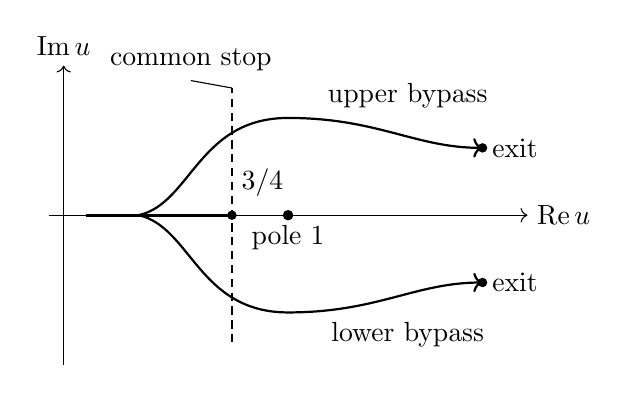
\begin{tikzpicture}[scale=0.95]
  \draw[->] (-0.2,0)--(6.2,0) node[right] {\(\operatorname{Re}u\)};
  \draw[->] (0,-2.0)--(0,2.0) node[above] {\(\operatorname{Im}u\)};
  \draw[densely dashed] (2.25,-1.7)--(2.25,1.7);
  \node[above right] at (2.25,0.12) {\(3/4\)};
  \fill (3,0) circle (2pt) node[below] {pole \(1\)};
  \draw[thick,->] (0.3,0)--(1.0,0)
    .. controls (1.7,0.15) and (1.8,1.3) .. (3.0,1.3)
    .. controls (4.2,1.3) and (4.7,0.9) .. (5.6,0.9);
  \draw[thick,->] (1.0,0)
    .. controls (1.7,-0.15) and (1.8,-1.3) .. (3.0,-1.3)
    .. controls (4.2,-1.3) and (4.7,-0.9) .. (5.6,-0.9);
  \draw[very thick] (0.3,0)--(2.25,0);
  \fill (2.25,0) circle (1.8pt);
  \node[above] (commonstop) at (1.7,1.8) {common stop};
  \draw[thin] (commonstop.south)--(2.25,1.7);
  \fill (5.6,0.9) circle (1.8pt) node[right] {exit};
  \fill (5.6,-0.9) circle (1.8pt) node[right] {exit};
  \node at (4.6,1.6) {upper bypass};
  \node at (4.6,-1.6) {lower bypass};
 \end{tikzpicture}
 \caption{Schematic only: the two bypasses can be curtailed and
 deformed to the thick real segment ending at the common pre-pole stop.
 The two artificial exits are marked.  The drawn curves are not
 the quantitative circle profiles; their admissibility is proved
 by \eqref{arr:circle-strict} and \eqref{arr:affine-homotopy}.}
 \label{arr:contour-schematic}
\end{figure}

Figure~\ref{arr:contour-schematic} shows the role of the common
pre-pole segment: curtailing both contour problems to that segment
allows uniqueness of the normalized solve to compare their actions.

\subsection{Prescribed finite graph gauges}\label{sec:gauges}

The reference-family construction used the radial, conical, and compact
coefficient maps.  The lateral paths additionally change between radius
and height variables and pass through long height charts near a collapsing
circular profile.  The estimates below retain each highest second
derivative in its bulk norm while controlling its coefficient by
first-derivative traces.

All complex geometric expressions below use the complex bilinear extension of
Euclidean products.  The parameters of a surface chart remain real.  A complex
contour is specified in its reference functions; it does not mean that an
unknown smooth function has been continued to a complex spatial argument.
Square roots of area elements are continued from the positive real branch.
The compact observation charts and their cutoffs remain fixed.

For an interval $I$ of length between two fixed positive constants, set
\begin{align}
 \|v\|_{\mathcal X_h(E;I)}={}&
 \|(v,v_t,v_{\theta\theta},E v_{tt},\sqrt E v_{t\theta})
                         \|_{L^2(I;H^h(\mathbb S^1))}
 \notag\\[-2pt]
 &+\|(v,v_\theta,\sqrt E v_t)\|_{L^\infty(I;H^h(\mathbb S^1))},
 \qquad
 \|f\|_{\mathcal Y_h(I)}=\|f\|_{L^2(I;H^h(\mathbb S^1))}.
 \label{gauge:norm}
\end{align}
Here and below $h\ge4$ is fixed.  The trace terms are supplied by
Lemma~\ref{lin:strip}; one can equivalently include them in the norm.
On overlapping intervals the weights $E$ are comparable, with bounded
normalized derivatives.  A uniformly local weighted norm is the supremum
of the strip norms after division by the chosen growth weight.  All estimates
in this subsection hold at any fixed larger angular order as well.

\begin{lemma}[Mixed prescribed gauges]\label{gauge:mixed}
Let $B\ge1$ and, on a bounded interval, prescribe smooth circular reference
functions and transverse coefficients
\begin{equation}
 X(t,\theta)=(B\zeta(t,\theta),R(t,\theta)e_r(\theta)),\quad
 \zeta=\zeta_0+c_1u,\qquad R=R_0+c_2u.
 \label{gauge:immersion}
\end{equation}
Assume that $R_0$, $\zeta_0'$ and
$c_2\zeta_0'-c_1R_0'$ are bounded away from zero, that their required
fixed derivatives are bounded, and that the circular reference has the
strict ellipticity margins of Lemma~\ref{lin:strip} after division by its
drift.  Constants may depend on these fixed margins.
Then the scalar stationary operator divided by the normal component of
$X_u$ is an analytic map from a sufficiently small
$\mathcal X_h(B^{-2})$ ball to $\mathcal Y_h$.
If $\|u\|_{\mathcal X_h(B^{-2})}\le W$ and $BW$ is sufficiently small,
its nonlinear remainder satisfies
\begin{equation}
 \|\mathcal Q(u)-\mathcal Q(0)-D\mathcal Q(0)u\|_{\mathcal Y_h}
       \le C_h(BW^2+B^2W^3).
 \label{gauge:mixed-bound}
\end{equation}
On that ball its Lipschitz constant, after subtraction of the linear part,
is at most $C_h(BW+B^2W^2)$.  Averaging the equation in these prescribed
coordinates gives the same bound for the defect of the circular mean curve.
These statements include all angular commutations through order $h$.
\end{lemma}

\begin{proof}
Write $a=\zeta_t$, $b=R_t$ and
\begin{equation}
 D=c_2a-c_1b
  =c_2\zeta_0'-c_1R_0'+(c_2c_1'-c_1c_2')u.
 \label{gauge:transverse}
\end{equation}
In particular $D$ contains neither $u_t$ nor $u_\theta$.
The tangent vectors give
\begin{align}
 g_{tt}&=B^2a^2+b^2=:A,
 &g_{t\theta}&=(B^2ac_1+bc_2)u_\theta,
 &g_{\theta\theta}&=R^2+(B^2c_1^2+c_2^2)u_\theta^2,\notag\\
 J:=\det g&=R^2A+B^2D^2u_\theta^2,
 &g^{tt}&=\frac{R^2+(B^2c_1^2+c_2^2)u_\theta^2}{J},\notag\\
 g^{t\theta}&=-\frac{(B^2ac_1+bc_2)u_\theta}{J},
 &g^{\theta\theta}&=\frac A J.
 \label{gauge:metric}
\end{align}
The cancellation in the determinant is exact.  In particular, a term
$B^2\zeta_\theta^2$ cannot be estimated independently of the off-diagonal
square in the determinant.  For $E=B^{-2}$, $d=a^2+Eb^2$,
$L=c_1a+Ec_2b$ and $T=R^2d+D^2u_\theta^2$, the same identities become
\begin{equation}
 g^{tt}=\frac E d+\frac{L^2u_\theta^2}{dT},\qquad
 g^{t\theta}=-\frac{Lu_\theta}{T},\qquad
 g^{\theta\theta}=\frac dT,\qquad
 g^{tt}-\frac{(g^{t\theta})^2}{g^{\theta\theta}}=\frac E d.
 \label{gauge:schur}
\end{equation}
This is the exact Schur complement identity.

An unnormalized normal, sufficient for taking normal components, is
\begin{equation}
 N=\left(-b/B,\ a e_r+
          \frac{b\zeta_\theta-aR_\theta}{R}e_\theta\right).
 \label{gauge:normal}
\end{equation}
It satisfies $N\cdot X_t=N\cdot X_\theta=0$ and $N\cdot X_u=D$.
Consequently the stationary equation is precisely
\begin{equation}
 \mathcal Q(u)=g^{ij}\frac{N\cdot X_{ij}}D
                         +\frac{N\cdot X}{2D}=0.
 \label{gauge:operator}
\end{equation}
No connection term remains in $N\cdot X_{ij}$.  Direct differentiation yields
\begin{align}
 \frac{N\cdot X_{tt}}D&=u_{tt}+C_{tt},
 &C_{tt}&=\frac{a(R_0''+c_2''u+2c_2'u_t)
                    -b(\zeta_0''+c_1''u+2c_1'u_t)}D,\notag\\
 \frac{N\cdot X_{t\theta}}D&=u_{t\theta}+C_{t\theta}u_\theta,
 &C_{t\theta}&=\frac{ac_2'-bc_1'}D-\frac bR,\notag\\
 \frac{N\cdot X_{\theta\theta}}D
        &=u_{\theta\theta}-\frac{aR}D-\frac{2c_2u_\theta^2}R,
 &\frac{N\cdot X}{D}&=\frac{Ra-\zeta b}D.
 \label{gauge:numerators}
\end{align}
Thus the complete operator is affine in the second derivatives.
$C_{tt}$ is at most quadratic in $u_t$ and $C_{t\theta}$ at most affine
in $u_t$, with coefficients analytic in $u$.  Moreover
\begin{align}
 Ra-\zeta b={}&R_0\zeta_0'-\zeta_0R_0'
 +(c_2\zeta_0'+R_0c_1'-c_1R_0'-\zeta_0c_2')u\notag\\
 &+(R_0c_1-\zeta_0c_2)u_t+(c_2c_1'-c_1c_2')u^2.
 \label{gauge:support}
\end{align}
The terms $u u_t$ cancel.  The normalized support function is affine in
$u_t$.  At circular data, irrespective of its speed,
\begin{equation}
       g^{tt}=A^{-1}=O(B^{-2}),\qquad
       g^{t\theta}=0,\qquad g^{\theta\theta}=R^{-2}.
 \label{gauge:circular-cancellation}
\end{equation}
In particular the circular angular curvature term is $-a/(DR)$,
which is affine in $u_t$; it has no unsuppressed quadratic speed term.

Here is a full coefficient estimate.  Use the Banach algebra
$\mathcal A=L^\infty(I;H^h(\mathbb S^1))$ and its module
$\mathcal Y_h$.  By \eqref{gauge:norm},
\begin{equation}
 \begin{gathered}
 \|(u,u_\theta)\|_{\mathcal A}\le W,\qquad
 \|u_t\|_{\mathcal A}\le BW,\\
 \|(u_t,u_{\theta\theta})\|_{\mathcal Y_h}\le W,\qquad
 \|u_{t\theta}\|_{\mathcal Y_h}\le BW,\qquad
 \|u_{tt}\|_{\mathcal Y_h}\le B^2W.
 \end{gathered}
 \label{gauge:slots}
\end{equation}
The functions $R,D,d,T$ are analytic units in this algebra when $BW$
is small.  Equations \eqref{gauge:schur}--\eqref{gauge:numerators}
partition the entire operator into the following classes:
\begin{enumerate}
\item The circular radial coefficient is $E$ times an analytic function
of $(u,u_t)$.  Its change multiplies $u_{tt}$ with bound
$C E(W+BW)B^2W\le CBW^2$.
Its Taylor terms on bounded reference derivatives satisfy this bound too.
\item Every extra radial coefficient has two factors $u_\theta$, by
\eqref{gauge:schur}.  Its product with $u_{tt}$ is bounded by $CB^2W^3$.
\item The mixed coefficient has a factor $u_\theta$ and analytic dependence
on $(u,u_t,u_\theta)$.  Its product with $u_{t\theta}$ is $O(BW^2)$;
any additional speed factor costs at most $BW$.
\item The angular coefficient equals $R^{-2}$ plus a term divisible by
$u_\theta^2$.  Its change multiplying $u_{\theta\theta}$ is
$O(W^2)+O(W^3)$, with analytic speed factors uniformly bounded.
\item The remaining terms are exactly the lower terms in
\eqref{gauge:numerators} and \eqref{gauge:support}.
Pure speed squares in $C_{tt}$ retain the factor $E$; all other pure
speed dependence at $u_\theta=0$ is affine.  Terms with angular tilt
retain its one or two explicit factors.  A product containing only
first derivatives is estimated with one factor in $\mathcal Y_h$,
so even $u_t^2$ costs $BW^2$, rather than $B^2W^2$.
\end{enumerate}
This list exhausts the three inverse-metric contractions and the support
term.  Every further Taylor factor is small in $\mathcal A$, being
bounded by $C(W+BW)$.  The convergent analytic series therefore sum to
\eqref{gauge:mixed-bound}.  Differencing a product gives the asserted
Lipschitz estimate.  The multiplication inequality
$\|fg\|_{H^h}\le C_h\|f\|_{H^h}\|g\|_{H^h}$ proves these statements
with all $h$ angular commutations, keeping exactly one second derivative
in $L^2$; none is put into a trace.

For the last assertion let $U=\langle u\rangle_\theta$ and
$\mathcal N(u)=\mathcal Q(u)-\mathcal Q(0)-D\mathcal Q(0)u$.
The linearized coefficients are independent of $\theta$, whence
\begin{equation}
 \mathcal Q(U)=\mathcal N(U)-\langle\mathcal N(u)\rangle_\theta
 \quad\hbox{if }\mathcal Q(u)=0.
 \label{gauge:averaging}
\end{equation}
The circular curve is exactly $(B(\zeta_0+c_1U),R_0+c_2U)$.
If instead one expands about $U$, its second derivatives need not have
uniform traces: split them into reference derivatives and perturbation
derivatives and keep the latter in the same $L^2$ slot.  The coefficient
Taylor remainder then costs at most $B^2W^3$.  This proves the claim also
for a varying circular mean.
\end{proof}

\begin{lemma}[Long polar height charts]\label{gauge:height}
Prescribe the polar height chart
\[
 X=(Zg(r,\theta),r e_r(\theta))
\]
on real parameters along a fixed complex $r$ contour.  Let $|Z|\asymp B$,
$t=-\log r$, and assume a uniformly bounded circular reference $g_0$ satisfies
$|(g_0)_t|\asymp |r|^2$, with its fixed log derivatives of this size.
Assume $|Br|\ge Y_0$ and put $E=|Br|^{-2}$ on each strip.  The reference
conditions include the full real pullback and drift division.  More precisely,
if $t=t(\xi)$ on the real outward parameter and $J=t_\xi$, assume
$J,J^{-1}$ and their required fixed derivatives are bounded.  Let
$\mathcal F_t(g)$ denote the left side of the log-normalized equation
\eqref{gauge:polar-normalized} below, including its graph-dependent
$H_1$ division.  Write its circular linearization in the log coordinate as
\[
 D\mathcal F_t(g_0)v=(1+d_{\mathrm{ref}})v_t-a_{\mathrm{ref}}v_{tt}
       -c_{\mathrm{ref}}v_{\theta\theta}+q_{\mathrm{ref}}v.
\]
Its full pulled drift is
$\Delta_{\mathrm{ref}}=1+d_{\mathrm{ref}}
             +a_{\mathrm{ref}}J_\xi/J^2$.
Assume this is a bounded unit and that, after division by it,
\[
 \operatorname{Re}\frac{a_{\mathrm{ref}}}{J\Delta_{\mathrm{ref}}}\ge cE,
 \quad \left|\frac{a_{\mathrm{ref}}}{J\Delta_{\mathrm{ref}}}\right|\le CE,
 \quad \operatorname{Re}\frac{Jc_{\mathrm{ref}}}{\Delta_{\mathrm{ref}}}\ge c,
 \quad \left|\frac{Jc_{\mathrm{ref}}}{\Delta_{\mathrm{ref}}}\right|\le C.
\]
The normalized coefficient derivatives and lower terms satisfy the bounds
of Lemma~\ref{lin:strip}.  All metric and graph denominators in
$\mathcal F_t$ remain bounded analytic units in their normalized scales
on the graph neighborhood.  These are algebraic hypotheses
on the prescribed reference, checked for the collapsing paths below.
Let $\operatorname{pb}_J$ mean the algebraic pullback obtained by replacing
$\partial_t$ with $J^{-1}\partial_\xi$ and reading all prescribed
coefficients along the real path.  We use the fixed circular row
\begin{equation}\label{gauge:fixed-row}
 \mathcal F_{\mathrm{norm}}(g)
   =\Delta_{\mathrm{ref}}^{-1}J\,\operatorname{pb}_J\mathcal F_t(g).
\end{equation}
In particular $\Delta_{\mathrm{ref}}$ is held fixed when this map is
linearized at the possibly nonexact profile $g_0$.  This circular row
depends only on $\xi$, so it preserves mean and oscillatory projections.
All strip norms use
the real parameter $\xi$ after this pullback.  Take $Y_0$ large.  The map
$\mathcal F_{\mathrm{norm}}$ is analytic whenever
\begin{equation}
 \frac{E^{-1/2}}{|r|^2}(W_m+W_o)\ll1,
 \qquad
 \frac{E^{-1/2}}{|r|^2}W_o\ll1,
 \label{gauge:height-small}
\end{equation}
where $v=g-g_0$ has mean and oscillation of
$\mathcal X_h(E)$ sizes $W_m,W_o$ respectively.
Writing $W=W_m+W_o$, its remainder
$\mathcal N(v)=\mathcal F_{\mathrm{norm}}(g_0+v)
-\mathcal F_{\mathrm{norm}}(g_0)-D\mathcal F_{\mathrm{norm}}(g_0)v$ obeys
\begin{equation}
 \|\mathcal N(v)\|_{\mathcal Y_h}
 \le C_h\left(\frac{E^{-1/2}}{|r|^2}W^2
              +\frac{E^{-1}}{|r|^4}W_o^2W\right).
 \label{gauge:height-bound}
\end{equation}
With $A_r=E^{-1/2}/|r|^2$ and $C_r=E^{-1}/|r|^4$, its mean and
oscillatory outputs satisfy, respectively,
\begin{align}
 \|\langle\mathcal N(v)\rangle\|_{L^2_\xi}
       &\le C_h\{A_r(W_m^2+W_o^2)+C_rW_o^2W\},\notag\\
 \|\mathcal N(v)-\langle\mathcal N(v)\rangle\|_{\mathcal Y_h}
       &\le C_h\{A_r W_oW+C_rW_o^2W\}.
 \label{gauge:height-projections}
\end{align}
The corresponding multilinear difference estimates hold.  These estimates
are uniform at each fixed angular order.
\end{lemma}
\begin{proof}
The physical slopes in the polar orthonormal frame are
$p=-Zg_t/r$, $q=Zg_\theta/r$.  With $H=1+p^2+q^2$, the curvature
matrix has entries
\begin{equation}
 A=\frac{1+q^2}{H},\qquad D_\theta=\frac{1+p^2}{H},\qquad
 C=-\frac{pq}{H}.
 \label{gauge:polar-matrix}
\end{equation}
The stationary equation, multiplied by $r^2/Z$, is exactly
\begin{equation}
 A(g_{tt}+g_t)+D_\theta(-g_t+g_{\theta\theta})
 -2C(g_{t\theta}+g_\theta)
       =-\tfrac12r^2(g_t+g).
 \label{gauge:polar-equation}
\end{equation}
Complex tangent factors on a prescribed contour are included by the chain
rule in \eqref{gauge:fixed-row}.  Its row is the fixed circular unit,
including the $J_\xi$ term; the graph-dependent $H_1$ normalization remains
inside $\mathcal F_t$ and its linearization.  The preceding normalized
inequalities retain the required strict margins.

Set $p_0=-Z(g_0)_t/r$, $e=p_0^{-2}$, $s=(p-p_0)/p_0$ and $q=p_0 v_1$.
Then $|e|\asymp E$, $s= v_t/(g_0)_t$ and
$v_1=-v_\theta/(g_0)_t$, and the exact coefficient formulas read
\begin{equation}
 A=\frac{e+v_1^2}{e+(1+s)^2+v_1^2},\quad
 D_\theta=\frac{e+(1+s)^2}{e+(1+s)^2+v_1^2},\quad
 C=-\frac{(1+s)v_1}{e+(1+s)^2+v_1^2}.
 \label{gauge:relative-coefficients}
\end{equation}
For an explicit check of the drift division, write instead
$P=g_t/r^2$, $Q=g_\theta/r^2$, $e_1=(Zr)^{-2}$ and
\[
 H_1=(1-r^2/2)P^2-(1+r^2/2)Q^2-r^2e_1/2.
\]
Equation~\eqref{gauge:polar-equation} becomes
\begin{equation}
 g_t-a_1g_{tt}-b_1g_{\theta\theta}
       +2c_1^*g_{t\theta}+2c_1^*g_\theta-d_1g=0,
 \label{gauge:polar-normalized}
\end{equation}
where
\[
 a_1=\frac{e_1+Q^2}{H_1},\qquad
 b_1=\frac{e_1+P^2}{H_1},\qquad
 c_1^*=\frac{PQ}{H_1},\qquad
 d_1=\frac{r^2(e_1+P^2+Q^2)}{2H_1}.
\]
Here $P$ is a bounded unit at the reference.  Put
$\mathfrak p=E^{-1/2}W/|r|^2$ and
$\mathfrak q=E^{-1/2}W_o/|r|^2$.  In the angular algebra these exact
normalized coefficients satisfy
\begin{equation}
 \frac{\|a_1-a_{1,0}\|}{E}
 +\frac{\|b_1-b_{1,0}\|}{E}
 +\frac{\|d_1-d_{1,0}\|}{|r|^2E}
 \le C(\mathfrak p+\mathfrak q^2),\qquad
 \frac{\|c_1^*\|}{\sqrt E}\le C\mathfrak q.
 \label{gauge:relative-normalized}
\end{equation}
In particular at zero tilt the speed variation of $b_1$ retains a
factor $E$, and that of $d_1$ a factor $r^2E$; their remaining variations
have two tilt factors.  Drift division introduces no unweighted
radial-speed term.

Consequently $A-A_0=O(E s)+O(v_1^2)$,
$D_\theta-1=-v_1^2/(e+(1+s)^2+v_1^2)=O(v_1^2)$, and
$C=O(v_1)$, as analytic algebra estimates.
Every pure radial-speed variation in $A$ retains the factor $E$;
angular changes of $A$ have two tilt factors.  The condition that the
mixed coefficient be small relative to $\sqrt E$ is precisely the
second smallness condition in \eqref{gauge:height-small}.

For the full map, assign the traces of $v,v_\theta$ size $W$, the trace
of $v_t$ size $E^{-1/2}W$, and the bulk sizes of
$v_{tt},v_{t\theta},v_{\theta\theta}$ respectively
$E^{-1}W,E^{-1/2}W,W$.  A pure speed change in $A$ times $v_{tt}$ is
bounded by
$E|r|^{-2}(E^{-1/2}W)(E^{-1}W)=A_rW^2$.
A mixed tilt times $v_{t\theta}$ costs $A_rW_oW$.
The two-tilt part of $A$ times $v_{tt}$ costs $C_rW_o^2W$.
The angular coefficient costs less.  These are all second derivative
terms in \eqref{gauge:polar-equation}.
For a coefficient Taylor remainder on a background derivative, use its
size $O(|r|^2)$.  The pure speed part has the factor $E$, and use one
$v_t$ in bulk rather than trace.  For instance
$E|r|^{-4}v_t^2 O(|r|^2)$ has bound
$E^{1/2}|r|^{-2}W^2\le A_rW^2$.
Tilt squares have bound $|r|^{-2}W_o^2\le A_rW_o^2$.
For the normalized zeroth-order term $d_1g_0$, use the factor $r^2E$
in \eqref{gauge:relative-normalized} and $g_0=O(1)$, giving these same
bounds; it is not necessary to assign $g_0$ the derivative size $O(r^2)$.
All lower terms are already displayed in \eqref{gauge:polar-equation};
the support term before division is affine in $g,g_t$.
The analytic $H_1$ division already included in $\mathcal F_t$ preserves
these bounds by its unit expansion.  The fixed row in
\eqref{gauge:fixed-row} and its bounded chain-rule coefficients preserve
them as well.  Higher powers are absorbed using
\eqref{gauge:height-small}.

Finally rotation of $\theta$ commutes with the equation.  At a circular
input, its linearization has circular coefficients.  A mean output
therefore has no term linear in the oscillation, and an oscillatory output
has no term containing only mean inputs.  Applying the preceding
multilinear estimates with these absent terms gives
\eqref{gauge:height-projections}.  Analytic composition in $H^h$ and the
single highest-derivative bulk slot prove every angular commutation and
every difference estimate asserted above.
\end{proof}

\subsection{A uniform normalized inverse on finite contours}
\label{sec:finite-linear}

The infinite-end estimates now have to be combined with the long
prescribed paths.  Compact observations remove the Gaussian kernel;
the weighted end estimate must also prevent an approximate kernel
from escaping toward a receding endpoint.  We use the compact norms
and coefficient maps of \Cref{gauge:compact}, and the finite graph
calculations of \Cref{gauge:mixed,gauge:height}.  The end weights are
retained until the final conversion to physical graph bounds.

Here is the geometry behind the parameters in the next proposition.
The large number $B$ measures axial distance along a cylindrical end;
in the later application it is the inverse square root of the opening
scale.  The fixed number $D$ bounds the size of a contour after division
of axial distances by $B$.  A polar height chart writes the surface as
$X=(Zg(r,\theta),r e_r(\theta))$, with $|Z|\asymp B$ and
$e_r(\theta)=(\cos\theta,\sin\theta)$.  Its scalar variable $g$ is
height divided by $Z$, and $r_0$ is its entrance radius; decreasing $r$
corresponds to increasing $\log(r_0/r)$.  A prescribed complex path is
given by $r=r(s)$ on a real outward parameter interval.  The complex
quantity $\log(r_0/r(s))$ occurs only through its coefficients and
chain rule; it is not a new spatial domain.
An outgoing derivative condition prescribes the first derivative of
this scalar graph variable at the terminal section of that interval.
The proposition states the precise analytic hypotheses independently
of any particular contour construction.

\begin{proposition}[Weighted normalized inverse]\label{lin:global}
Fix an angular order $h$, a finite geometric parameter $D$, a cylindrical
weight rate $\alpha_{\mathrm{cyl}}>2.1$, and the
compact observations from Lemma~\ref{lin:observations}.  Consider surfaces of
parameter size $B\to\infty$, obtained by replacing far cylindrical
pieces by real-parameter paths with complex coefficients, optionally
followed by height charts of length $O(\log B)$.  The conical ends may
remain infinite.  The following are the hypotheses on the linear
operators and prescribed charts.

\begin{enumerate}
 \item On each fixed compact subset, the coefficients, compact
 multiplier sources, and observations converge smoothly to
 \eqref{lin:augmented}, or to a member of a sufficiently small uniformly
 invertible perturbation of that block.
 \item From a fixed entrance to $z=cB$, the cylindrical operator is a
 sufficiently small perturbation of
 \eqref{lin:cylinder-operator}.  Choose $c>0$ so that a propagation
 rate $2.1$ is available.  Beyond that point, bounded bands of length
 depending on $D$ satisfy Lemma~\ref{lin:strip}.  A height chart is the
 real-parameter pullback of $\tau=\log(r_0/r)$, with
 $E\asymp(B|r|)^{-2}$, ending with
 $B|r|\ge Y_0$.  Its coefficients obey the same accretivity, derivative,
 lower-term, and small-perturbation bounds.
 \item Each modified cylindrical end has one ordered real outward
 interval $[s_0,T_B]$, equal to the original log coordinate on its
 long real part.  Local real outward coordinates on overlaps are
 $t_i=\chi_i(s)$ with $0<c\le\chi_i'\le C$ and bounded required
 fixed derivatives; the real angular coordinate is unchanged.
 There is a positive scale $E_B(s)$ comparable to the local scales
 with bounded logarithmic derivatives.  The prescribed scalar
 variables are descriptions of one scalar variable through transition
 factors $A_i(s,\theta)$ on fixed overlap bands.  The functions
 $A_i,A_i^{-1}$ and their ordinary real-coordinate derivatives through
 the required fixed orders are bounded.  Choose this scalar variable
 to agree with each prescribed long-chart variable off those bands and
 with the prescribed exit variable near $T_B$.  After these changes,
 the normalized reference operators and their source rows are smooth
 restrictions of one operator on the interval; any additional terms
 from the actual backgrounds satisfy the bounded lower-term and small
 domain-to-range perturbation hypotheses in (ii).  These requirements
 exclude distributional seams.  The coefficients on conical ends satisfy
 Lemma~\ref{lin:conical}, up to a small domain-to-range perturbation.
 \item For each fixed $B$ and sufficiently remote finite stops on
 the conical ends, fixed domain and range isomorphisms identify the
 actual stopped operator with an operator connected to a real
 coercive scalar elliptic problem by an operator-norm continuous homotopy
 on the fixed compact $H^2$ domain with homogeneous boundary
 conditions and range $L^2$. Its coefficients and boundaries are smooth,
 its symbols are properly elliptic, and its boundary conditions are
 complementing throughout. The equal-dimensional
 compact observation and multiplier augmentation is retained.
 This is only an index hypothesis: the uniform estimates in the
 preceding items are required for the actual operators, not for
 the artificial operators along the homotopy.
\end{enumerate}

For clarity, the coefficient requirement in (iii) includes the tangent
of every prescribed complex log path.  If $t=t(s)$ is such a log and
$H=t_s$ is its complex tangent, independent of $\theta$, then the chain
rule on the real $s$ interval gives
\begin{equation}\label{lin:complex-log-pullback}
 \begin{split}
 H\mathcal L={}&\partial_s-\frac aH\partial_{ss}
       -2b\partial_{s\theta}-Hc\partial_{\theta\theta}\\
 &+\left(d_1+\frac{aH_s}{H^2}\right)\partial_s
       +Hd_2\partial_\theta+Hd_0,
 \end{split}
\end{equation}
and the source is multiplied by $H$.  Thus $H,H^{-1}$ and its required
fixed derivatives, including $H_s$, must be bounded.  If the full drift
is divided out, its divisor is
$\delta_H=1+d_1+aH_s/H^2$, and the actual inequalities in (ii) are
\[
 \operatorname{Re}\frac{a}{H\delta_H}\ge cE_B,\quad
 \operatorname{Re}\frac{Hc}{\delta_H}\ge c,\quad
 \left|\frac{a}{H\delta_H}\right|\le CE_B,\quad
 \left|\frac{Hc}{\delta_H}\right|\le C,\quad
 \left|\frac b{\delta_H}\right|\le\varepsilon_*\sqrt{E_B}.
\]
The divided source is $Hf/\delta_H$.  A nonzero divisor alone does not
imply these real-part inequalities.  If $\delta_H=1+O(E_B)$, its
closeness to one preserves previously fixed strict margins.

Choose a weight $\rho_B$ with rate $\alpha_{\mathrm{cyl}}$ on the long real cylinder,
a sufficiently large fixed rate $d_D$ on the bounded modified bands,
and a sufficiently large fixed rate $d_{\mathrm{cap}}$ on a height
chart, retaining its value at the entrance of each new chart.  All
rates exceed their propagation rates by fixed positive margins, are at
least $\alpha_{\mathrm{cyl}}$, and
their interpolations occupy fixed overlap bands where the adjacent
coefficient estimates both hold.  Choose $Y_0$ after these
rates so that $d_{\mathrm{cap}}\sup E$ is sufficiently small; take $B$
large only after these choices.

Here $u$ denotes the scalar unknown in each prescribed chart: normal
height on the core, radius on cylindrical charts, relative height on
cap charts, and link displacement on conical charts.  The corresponding
source uses the same change of graph units and drift normalization.
Let $X_B$ consist of the compact norm \eqref{lin:compact-norm}, the
cylindrical and height norms \eqref{lin:weighted-strip}, the conical
norms \eqref{lin:conical-norm}, and the Euclidean norm of the compact
multiplier vector.  Let $Y_B$ consist of the corresponding compact
and end source norms and the Euclidean observation norm.  Homogeneous
outgoing graph-derivative conditions are included in the domain.
Then
\begin{equation}\label{lin:global-estimate}
 \|(u,\lambda)\|_{X_B}
 \le C_{D,Y_0,h,\alpha_{\mathrm{cyl}}}
 \left\|\bigl(L_Bu+\sum_i\lambda_i\chi_{i,B},P_Bu\bigr)\right\|_{Y_B},
\end{equation}
and this normalized operator is onto.  At a true terminal section define
$g=u_s(T_B)$ for the prescribed scalar variable in the real outward
coordinate.  If $t=t(s)$ is a local log coordinate, this means
$g=H u_t(T_B)$ with $H=t_s$.  For this prescribed exit derivative
the right hand side is augmented by
$\rho_B(T_B)^{-1}\|g\|_{\mathcal T^N_{E(T_B),h}}$ at each terminal section;
the sum over the fixed finite list of exits is understood.
The thresholds and constant may depend on the fixed rate, but are independent
of $B$ and of the lengths of the exhausted
conical ends.  Removing $\rho_B$, or converting a relative height
to physical height on a cap, costs at most a fixed power of $B$.
The preliminary construction uses $\alpha_{\mathrm{cyl}}=2.2$; a source
with a fixed higher Taylor growth rate is permitted by choosing
$\alpha_{\mathrm{cyl}}$ equal to or larger than that rate.  The strict
buffer is above the propagation rate, so equality with the source growth
rate is allowed in the uniformly local source norm.
\end{proposition}

\begin{proof}
We first prove one exterior estimate on the real interval in (iii).
This avoids imposing boundary data at changes of graph gauge.  For a
scalar change $u=A\widetilde u$, conjugate the source by $A^{-1}$.
The principal coefficients of \eqref{lin:admissible-operator} are
unchanged, while the lower coefficients become
\begin{align*}
 \widetilde d_1&=d_1-2aA_s/A-2bA_\theta/A,\\
 \widetilde d_2&=d_2-2bA_s/A-2cA_\theta/A,\\
 \widetilde d_0&=d_0+(1+d_1)A_s/A+d_2A_\theta/A
       -aA_{ss}/A-2bA_{s\theta}/A-cA_{\theta\theta}/A.
\end{align*}
The $a$ contribution to $\widetilde d_1$ is $O(E_B)$; the
$b$ contribution is $O(\varepsilon_*\sqrt{E_B})$ and is an allowed
small strip operator perturbation.  The remaining additions are bounded
lower terms.  In particular $A_s/A$ must have an ordinary bounded
derivative norm, since it occurs without an $E_B$ factor in the mass.
The transition is taken in the prescribed reference frames; the
coefficient--module bounds control the rougher actual backgrounds.
For the one-dimensional real coordinate changes in (iii), the chain
rule is \eqref{lin:complex-log-pullback} with positive real $H$.
Their bounded factors preserve the radial, mixed, and angular units.

The fixed-radius radial-to-height transition illustrates why these
requirements hold for the later circular overlap.  Write
$z=Z_0\varphi(r)$ with $|Z_0|\asymp|Z|\asymp B$ and
$\varphi^2=1-r^2/2$, and put
$H_r=(\log(r_0/r))_s$.  Then
\[
 (\log z)_s=\frac{r^2}{2\varphi^2}H_r,\qquad
 u_{\rm rel}
       =-\frac{z_s}{Zr_s}u_{\rm radius}
       =\frac{Z_0}{Z}\frac r{2\varphi}u_{\rm radius}.
\]
Here $u_{\rm rel}$ is relative height, so the factor follows by equating
the two variations' normal components.
The last factor and its inverse have bounded fixed derivatives when
$|r|\asymp r_0>0$ and $\varphi$ is a unit.  They need not do so at
$|r|\asymp B^{-1}$, so the transition is made on that fixed-radius
overlap.  In the common real parameter, the circular radial and angular
diffusions, before the small axial-curvature correction to the drift, are
\[
 \frac{4}{Z_0^2r^2H_r(1+4\varphi^2/(Z_0^2r^2))},
       \qquad \frac{H_r}{\varphi^2}.
\]
These have the polar units $E_B\asymp(B|r|)^{-2}$ and $1$.
Equivalently, in the mixed gauge of Lemma~\ref{gauge:mixed}, the
angular-curvature and support terms have slow drift
$-\varphi^2/(r^2H_r)$, independent of the prescribed transverse
direction.  The formulas follow from
$r_s=-rH_r$, $z_s=Z_0r^2H_r/(2\varphi)$ and the metric in
\eqref{gauge:metric}.  The remaining axial drift is $O(E_B)$ on this
overlap.  On a long height chart \eqref{lin:complex-log-pullback} and
the strict margins in (ii) are checked with its own scale
$(B|r|)^{-2}$, including the tangent derivatives.  No uniformly bounded
conversion to physical normal height along the whole cap is needed here.

Trivialize on the fixed overlap bands as in (iii), keeping the prescribed
exit variable.  Put $u=\rho_B w$ on the entire interval and
$d=(\log\rho_B)_s$.  On the long real cylinder the model shifted mass at
$d=\alpha_{\mathrm{cyl}}$ is
\[
 d-2-2\mu^2(d^2-d).
\]
It has a strict positive buffer for a far entrance depending on this fixed
rate; at $d=2.2$ the limiting buffer is $0.2$.  The small full
operator-norm perturbation in (ii) preserves this estimate by absorption;
decay of that perturbation is not needed on the interval $z\le cB$.
Raise the rate on a fixed band while this margin still holds, before
entering a region whose lower terms require $d_D$, and similarly enter
the height rate.  On the other bands the algebraic mass is
\[
 (1+\widetilde d_1)d-a(d^2+d_s)+\widetilde d_0.
\]
The chosen rate exceeds the bounded reaction costs, and $E_Bd\ll1$
controls both the quadratic term and the smooth interpolation term.
The coefficient--module perturbations are absorbed with the strict
local margins.  Perform the integration in the proof of
\eqref{lin:forward} once on this whole interval, including the same
additional exponentially decreasing localization centered at an arbitrary
strip.  There are only the true entrance and terminal boundary terms.
The exit variable is unchanged there, so its conjugated condition is
$w_s+d w=\rho_B(T_B)^{-1}g$ and has the favorable terminal sign already
computed.  The geometric strip sum is uniform in the interval length.
Local patch estimates recover every bulk term across the smooth overlap
bands.  We obtain
\begin{equation}\label{lin:exterior-global}
 \|u\|_{X_B(\mathrm{exterior})}
 \le C\left(C_h^2(u;K_{\mathrm{collar}})
       +\|L_Bu\|_{Y_B(\mathrm{exterior})}
       +\|g/\rho_B(T_B)\|_{\mathcal T^N_{E(T_B),h}}\right).
\end{equation}
The overlap constants depend only on the prescribed fixed data and $D$.
Lemma~\ref{lin:conical} supplies the
conical part of this estimate.  The compact multiplier sources are
absent on all sufficiently far collars.

Interior elliptic estimates on nested fixed collars, including the
commutations in \eqref{lin:compact-norm}, now yield
\begin{equation}\label{lin:compact-remainder}
 \|(u,\lambda)\|_{X_B}
 \le C\left(\|\mathcal A_B(u,\lambda)\|_{Y_B}
                    +\|u\|_{L^2(K')}+|\lambda|\right)
\end{equation}
for a fixed compact $K'$.  In particular the estimate has been proved
in the weighted norm, before any power of $B$ is spent.

For a fully stopped problem write $T$ for the smallest logarithmic
stopping coordinate on the conical ends.  If there are no conical
ends, omit $T$.  Suppose there were no thresholds $B_0,T_0$ and
constant $C$ giving \eqref{lin:global-estimate} whenever
$B\ge B_0$ and $T\ge T_0$.  We could then choose a failing sequence
with $B\to\infty$ and every conical stop tending to infinity.
Normalize its unknowns to have $X_B$ norm one
and its output to tend to zero.  Interior compactness and finite
dimensionality of the multipliers give a local limit $(u_\infty,
\lambda_\infty)$.  On every fixed cylindrical interval the weight is
eventually $e^{\alpha_{\mathrm{cyl}}(t-t_0)}$.  Consequently $u_\infty$ has at most
polynomial growth there.  On conical ends its ambient normal height
has at most linear growth, by \eqref{lin:conical-norm}.  The derivative
estimates give $u_\infty\in H^2_G$.  It solves the homogeneous limiting
normalized block and hence vanishes, together with its multipliers.
Local elliptic estimates upgrade this convergence sufficiently to
make the compact terms in \eqref{lin:compact-remainder} vanish.  The
latter inequality contradicts the normalization.  This is the
exclusion of escape along a long end: it uses the fixed strict buffer
in \eqref{lin:exterior-global}, and would not follow by normalizing an
unweighted estimate with a factor $B^q$.
The contradiction gives one bound on the entire quadrant
$B\ge B_0$, $T\ge T_0$.  Thus the subsequent conical exhaustion
may fix any $B\ge B_0$ before sending the conical stops to infinity.

Surjectivity is a separate argument. Stop all ends, including the
conical ends, at remote finite sections. At each fixed $B$ and each
fixed conical stopping radius, the compact scalar boundary problem is
realized from its homogeneous mixed-boundary $H^2$ domain to $L^2$.
The full boundary-data map is Fredholm by the complementing-boundary theorem
\cite[Chapter~1, Section~1, subsection~3, Theorem~1.1]{NP1994}, localized in
surface charts. Entrance Dirichlet and transverse derivative
conditions occur on disjoint boundary components $\Gamma_D,\Gamma_N$.
To pass to the stated
homogeneous realization, let $\mathcal B$ be the boundary trace map into
$\mathcal T=H^{3/2}(\Gamma_D)\oplus H^{1/2}(\Gamma_N)$ and choose its
bounded right inverse $R$ from fixed smooth collars.  The decomposition
$u=v+Rg$, $v\in\ker\mathcal B$, identifies the full map with
$(v,g)\mapsto(L_Bv+L_BRg,g)$.  A bounded triangular change in the range
reduces it to $\operatorname{diag}(L_B|_{\ker\mathcal B},I_{\mathcal T})$,
so the homogeneous realization is Fredholm with the same index.
Hypothesis (iv)
identifies its index with that of a real coercive problem, hence zero.
Continuity of the index and invariance under finite-rank perturbations
are the Banach-space facts in
\cite[Chapter~IV, Sections~5.2--5.3, Theorems~5.17 and~5.26]{Kato1995}.
Adding equally many multiplier variables and observation equations first
gives $\operatorname{ind}\operatorname{diag}(L_B,0_{\mathbb C^m})
=\operatorname{ind}L_B$.  The off-diagonal observation and source maps
are finite rank, so the augmented block still has index zero.

Apply the already proved weighted a priori estimate to the actual
stopped operator. Its constants are independent of the conical
stopping radii by Lemma~\ref{lin:conical} and the compact-limit
argument above. For sufficiently remote stops and large $B$ it
excludes a kernel: elliptic boundary regularity
\cite[Chapter~1, Section~1, subsection~3, Theorem~1.5]{NP1994}
first makes every
kernel element smooth, so the commuted estimate applies. The stopped
augmented operator is therefore bijective on this $H^2$--$L^2$
realization. For smooth sources its solution is smooth; the actual
commuted estimates then bound it in $X_B$ by the source in $Y_B$.
Approximation by smooth sources extends this inverse to the stated
angularly commuted spaces, with the same uniform bound. Thus no
identification of those spaces with an isotropic higher Sobolev
scale is needed. Let the conical stops tend to infinity, keeping $B$
fixed. The uniform conical estimates, weak compactness in their
weighted bulk spaces, and local elliptic compactness pass these
solutions to the infinite-conical domain. The prescribed compact
observations and finite cylindrical or height exits pass to the
limit as well. This proves surjectivity of the actual operator
with the asserted bound.

Only compact stopped problems enter the artificial index homotopy.
No uniform inverse along that homotopy, no geometric realization
of its intermediate operators, and no deformation of an infinite
conical boundary problem are required. Fixed-parameter elliptic
Fredholm theory supplies the index; the weighted estimates for the
actual geometric operators supply uniformity in $B$ and in the
conical exhaustion.

Finally the real-cylinder weight is at most $CB^{\alpha_{\mathrm{cyl}}}$, and bounded bands
cost a fixed factor depending on $D$.  By the stated length hypothesis and
the bounded real pullbacks, a cap has $s$-length at most
$C_{\mathrm{par}}\log B+C_{\mathrm{par}}$, with $C_{\mathrm{par}}$ fixed
before $B$.  Thus
$\sup\rho_B\le C_{D,Y_0,\alpha_{\mathrm{cyl}}}
 B^{\alpha_{\mathrm{cyl}}+C_{\mathrm{par}}d_{\mathrm{cap}}}$.
Conversions of the prescribed height units and any fixed number of
their derivatives add only fixed powers.  This proves the last
assertion without altering the uniform weighted estimate.
\end{proof}

\begin{lemma}[Exponential backward shielding]\label{lin:shielding}
On a fixed log-length overlap suppose the hypotheses of
Lemma~\ref{lin:strip} hold with $E\asymp B^{-2}$.  A solution of the
homogeneous difference equation with zero entrance value and
polynomially bounded farther data is, on every fixed earlier band
separated from those data, bounded by
\begin{equation}\label{lin:shielding-estimate}
 C B^M\exp(-cB^2)
\end{equation}
in the strip norm, with every fixed number of admissible derivatives.
The assertion is stable under the small coefficient perturbations in
the same shifted domain-to-range norms.  It holds with actual outgoing
derivative data as well as with a farther Dirichlet trace.
For holomorphic finite-parameter derivatives, the solution and the
displayed bound are assumed on an outer parameter ball and the derivatives
are evaluated on an inner ball whose distance from the outer boundary is at
least $cB^{-q}$ for fixed $c,q>0$.  For smooth contour derivatives,
the pulled-back differentiated operators and data must separately obey
the corresponding shifted bounds, with a fixed separation of the two
bands.
\end{lemma}

\begin{proof}
Put $Z=B$, $d=c_1Z^2$, $D=\partial_t+d$, and
$v=e^{d(t-T)}w$, with $d$ constant on the overlap.
Choose $c_1>0$ after the reference margins so that $d\sup E$ is
small.  All bulk norms below mean $L^2_tH^h_\theta$ on the fixed
overlap, or on a fixed enlarged patch.  The shifted reference energy
has mass $d-O(Ed^2)\ge cd$; the symbol and boundary argument of
\eqref{lin:forward} control
\[
 N_d(w):=d\|w\|+\|Dw\|+\|w_{\theta\theta}\|
           +\|ED^2w\|+\|\sqrt E D w_\theta\|.
\]
Mixed and imaginary terms use the small derivative energies exactly
as in that argument.  For clarity the first traces also have constants
independent of $Z$.  With $E$ replaced by its comparable patch value,
product integration gives
\begin{align*}
 E\|Dw\|_{L^\infty H^h}^2
 &\le C\bigl((E+Ed)\|Dw\|^2+\|Dw\|\,\|ED^2w\|\bigr),\\
 \|w_\theta\|_{L^\infty H^h}^2
 &\le C\|w_{\theta\theta}\|
                   \bigl((1+d)\|w\|+\|Dw\|\bigr).
\end{align*}
The ordinary product identity supplies the $w$ trace.  Hence
$(w,w_\theta,\sqrt E Dw)$ is bounded by $CN_d(w)$ in
$\mathcal A=L^\infty_tH^h_\theta$.  The term $d\|w\|$ is
retained in this estimate; no second derivative has a trace.

Explicitly, for a perturbation
$\delta aD^2+2\delta bD\partial_\theta+\delta c\partial_\theta^2
+pD+q\partial_\theta+r$, a sufficient coefficient--module norm is
\[
 \mathfrak M=\|\delta a/E\|_{\mathcal A}
 +\|\delta b/\sqrt E\|_{\mathcal A}+\|\delta c\|_{\mathcal A}
 +E^{-1/2}\|p\|+\|q\|+\|r\|.
\]
The last three norms are bulk norms: the preceding traces give the
operator bound $C\mathfrak M N_d(w)$.  Bounded lower coefficients
may also be estimated directly on their bulk slots.

Here is the shifted perturbation check for the geometric difference
operators used below.  In the mixed prescribed gauges of
Lemma~\ref{gauge:mixed}, suppose the two background perturbations
have norm at most $W$ in \eqref{gauge:norm}, and set
$\varepsilon=ZW\ll1$.  Relative to the circular reference,
\eqref{gauge:schur} and \eqref{gauge:slots} give, uniformly along
the averaged segment,
\[
 \|\delta g^{tt}\|_{\mathcal A}\le CE(\varepsilon+\varepsilon^2),
 \quad\|\delta g^{t\theta}\|_{\mathcal A}\le C\sqrt E\varepsilon,
 \quad\|\delta g^{\theta\theta}\|_{\mathcal A}\le C(W+W^2).
\]
Analytic drift division preserves the corresponding normalized bounds.
Applying these coefficients to $D^2w,Dw_\theta,w_{\theta\theta}$
costs at most $C(\varepsilon+\varepsilon^2)N_d(w)$.
Keeping $D$ intact includes the terms with $d^2w$ and $dw_\theta$.

The averaged Jacobian also differentiates the coefficients multiplying
a background second derivative.  Keep that derivative in its original
unshifted $L^2$ slot.  From \eqref{gauge:schur}--\eqref{gauge:slots},
the resulting coefficients of $Dw,w_\theta,w$ have respective
$L^2_tH^h_\theta$ bounds
$CW$, $C(\varepsilon+\varepsilon^2)$, and $CW$.
For example differentiating the circular radial coefficient costs
$CE$, and $\|u_{tt}\|\le CZ^2W$; differentiating its two-tilt
correction costs $CW$, giving $CZ^2W^2$ in the angular slot.
Use $\|Dw\|_{\mathcal A}\le CZN_d(w)$ and the other first traces
to bound all these module products by
$C(\varepsilon+\varepsilon^2)N_d(w)$.
The lower terms are precisely \eqref{gauge:numerators} and
\eqref{gauge:support}: pure speed squares retain $E$, and the
circular angular and support terms are affine in speed.
They obey the same bound.  Thus the full difference operator satisfies
\[
 \|e^{-d(t-T)}(L_*-L_{\rm ref})e^{d(t-T)}w\|_{L^2H^h}
 \le C(\varepsilon+\varepsilon^2)N_d(w).
\]
This is a module estimate, not pointwise control of every lower
coefficient.  In a pure radial chart the variables in
Lemma~\ref{gauge:radial} give the same argument, with any small
circular opening included in the reference.  The reference margins
and this shifted smallness are checked before applying the lemma:
smallness of the opening alone does not assert $ZW\ll1$ for the
correction relative to that reference.

Keep the actual exit condition throughout:
\begin{equation}\label{lin:robin}
 v_t(T)=g\quad\Longleftrightarrow\quad Dw(T)=g.
\end{equation}
For a reference fast root the lift denominator is
$(\lambda_+-d)+d=\lambda_+$, so the natural norm
\eqref{lin:neumann-trace} retains its gain.
For homogeneous data the principal terminal coefficient is
$d\operatorname{Re}a+(1-2d\operatorname{Re}a)/2=1/2$;
$d_1=O(E)$ adds only $O(E)$.
The full perturbation is inverted on this same Robin domain by a
Neumann series once its displayed relative norm is sufficiently small.
No trace of a rough lower coefficient is introduced.
A scalar conversion $v=A(t)\widetilde v$ changes both the interior
operator and the exit to
$(\partial_t+d+A_t/A)\widetilde w=g/A$.
Bounded invertible $A$ with the prescribed derivative bounds gives
equivalent shifted domains.  Returning to ordinary derivatives costs
only fixed powers of $Z$; commuted versions use the corresponding
differentiated coefficient--module bounds.

One may alternatively take the farther actual trace as Dirichlet
data, or cut off the solution near the far side and impose zero data
beyond the cutoff.  The resulting source is supported a fixed distance
to the right of the band being estimated.  The factor
$e^{d(t-T)}$ suppresses its effect there by $e^{-d\,\mathrm{gap}}$.
The shifted estimates have only polynomial losses, which proves
\eqref{lin:shielding-estimate}.  All operations occur in prescribed
charts.  On the inner parameter ball in the statement, Cauchy's estimate
for a derivative of order $j$ costs at most $C_jB^{qj}$, which preserves
the exponential.  A ball's radius by itself gives no estimate at points
arbitrarily close to its boundary.  Smooth contour parameters instead
require differentiation of the equation and its prescribed real-domain
pullback.  When those differentiated coefficients and data have the
stated polynomial bounds and their sources remain on the farther side,
the same shifted estimate applies to each differentiated equation.
\end{proof}

\begin{remark}\label{lin:two-inversions}
The uniform weighted inverse and its polynomial physical version have
different uses.  A refined exterior nonlinear problem must first be
solved in its own mean and angular-oscillation weights, using the
corresponding small Lipschitz constants.  If its entrance agrees with
a preliminary normalized solution, Lemma~\ref{lin:shielding} makes a
splice residual exponentially small.  Proposition~\ref{lin:global}
can then correct that residual even after all fixed polynomial losses.
Applying a coarse $B^q$ inverse directly to the original exterior
power-sized error would require a separate smallness argument and is
not an implication of the proposition.
\end{remark}

\subsection{Exact normalized solves and their action}

We state precisely the earlier analytic estimates used here.
Lemma~\ref{lin:strip} controls, on unit evolution strips and at a
fixed sufficiently high angular order,
\[
 u,\ u_t,\ u_{\theta\theta},\ E u_{tt},\ \sqrt E\,u_{t\theta}
 \quad\hbox{in }L^2_tH^h_\theta,
 \qquad u,\ u_\theta,\ \sqrt E\,u_t\quad\hbox{as traces}.
\]
The coefficients must have radial and angular diffusion comparable
to \(E\) and \(1\), strictly positive normalized real parts, bounded
normalized derivatives, and mixed coefficient \(o(\sqrt E)\).
Proposition~\ref{lin:global} supplies an invertible augmented block
including the compact observations and multipliers, in uniformly
local growth-weighted versions of these norms.  On a cylindrical
piece the weight has a rate strictly above \(2\), with a positive
buffer above the propagation rate; bounded terminal bands use a
fixed larger rate if necessary.  The conical norms are those of
\Cref{lin:conical}, with the compact commutations used in
\Cref{lin:global}.  The inverse constant is
uniform in \(B\) with these weights retained.  Its physical norm,
and any fixed number of contour or finite-parameter derivatives,
may have fixed polynomial losses.  Exits are pure graph charts
with the outgoing derivative trace prescribed.  The fast Neumann
lift gains \(O(\sqrt E)\) in strip size relative to smooth fixed
angular-order derivative data.  Under conjugation the exit is the
corresponding Robin condition, as in Lemma~\ref{lin:shielding}.

Finally, Lemmas~\ref{gauge:mixed} and \ref{gauge:compact}
give analyticity of the complete prescribed-gauge map,
including the compact transition charts.
On a bounded scaled band, for strip size \(W\) and \(E\asymp B^{-2}\),
its nonlinear remainder and difference are bounded by
\begin{equation}\label{arr:tame-interface}
 C(BW^2+B^2W^3),\qquad
 C(BW+B^2W^2)\|u-\widetilde u\|.
\end{equation}
Second derivatives remain in the strip \(L^2\) factor and first
derivatives in the available traces; these estimates hold at the
full fixed angular order.  Thus they are estimates for the full
operator.  On height bands the corresponding estimate is
Lemma~\ref{gauge:height}.  In the present preliminary construction
only bounded scaled gauge changes are needed.

Here is the exit-data class for that construction.  Let $g_{\rm app}$
be the outgoing derivative of its comparison graph in the prescribed
pure exit variable, after the fixed graph-unit conversion.  If $T$ is
the exit and $\rho_B$ the growth weight of \Cref{lin:global}, permit
exactly the data satisfying
\begin{equation}\label{arr:allowed-traces}
 \rho_B(T)^{-1}
 \|g-g_{\rm app}\|_{\mathcal T^N_{E(T),h}}
       \le c_{\rm exit}B^{-4}.
\end{equation}
For fixed $s$ and contour parameters, use the prescribed real pullbacks
to identify each exit with a fixed boundary circle, and choose the
reference scales $E(T)$ and $\rho_B(T)$ independently of $p$ on the
outer parameter ball.  The varying geometric scales are uniformly
comparable there.  Let $\mathfrak T_B$ be the product of these complex
trace spaces, with norm the maximum of the left-hand norms in
\eqref{arr:allowed-traces}, and write
$\delta g=(g-g_{\rm app})_{\rm exits}$.  The fixed constant
$c_{\rm exit}$ is chosen for the finite collection of homotopies under
consideration, with a fixed factor of room in the contraction
construction.  Along a smooth contour homotopy the same bound holds
for its values, while each required derivative of its normalized
coefficients and data has a fixed polynomial bound.  The natural trace
norm is part of the inverse, so no unproved angular trace is used in
lifting these data.

We also fix the parameter reserve used below.  For constants
$0<c_{\rm in}<c_{\rm out}$ and an exponent $L$, put
\begin{equation}\label{arr:parameter-reserve}
 \mathcal B_s^{\rm out}=\{|p-p_0(s)|<c_{\rm out}|s|^L\},
 \qquad
 \mathcal B_s=\{|p-p_0(s)|<c_{\rm in}|s|^L\}.
\end{equation}
Solves are constructed on the outer ball and all uniform fixed
parameter derivatives are evaluated on the inner ball.  Cauchy's
estimate then costs only a fixed power of $|s|^{-1}$ at each fixed
order.  The finitely many later ball and sector restrictions are chosen
at once; their sectors retain an excess
$\delta_{\rm use}=\vartheta_\delta\delta\asymp D^{-1/2}$ for one fixed
$0<\vartheta_\delta<1$.

\begin{proposition}[Preliminary normalized arrays]\label{arr:preliminary-solves}
Fix \(D\), the bounded scaled portions of the contour families of
Lemma~\ref{arr:contours}, and a fixed lower radius \(r_*>0\).
Let \(p_0(s)\) be a sufficiently high polynomial truncation of
\(\widehat p(s)\).  For some fixed \(L\) and outer ball in
\eqref{arr:parameter-reserve}, for every \(p\in\mathcal B_s^{\rm out}\)
and every choice of outgoing data in \eqref{arr:allowed-traces} at
the artificial exits, the normalized stationary problem on either
contour family has a unique solution in the perturbative neighborhood.
For each fixed contour, the solution operator is jointly holomorphic
in \(p\) and an independent complex trace remainder
\(\delta g\in\mathfrak T_B\) for \(p\in\mathcal B_s^{\rm out}\) and
\(\|\delta g\|_{\mathfrak T_B}<c_{\rm hol}B^{-4}\), with a fixed
\(c_{\rm hol}>c_{\rm exit}\).  Hence a chosen \(p\)-dependent datum gives a holomorphic
solution when \(\delta g(p)\) is holomorphic into that fixed trace
space and remains in the stated trace ball on \(\mathcal B_s^{\rm out}\).
Smooth contour families with smooth prescribed data give
smooth solution families.  Every allowed solution lies in the
growth-weighted augmented ball
\[
 \|(u,\lambda)-(u_{\rm app},\lambda_{\rm app})\|_{X_B}
       \le C_{\rm pre}B^{-4},
\]
where the fixed $C_{\rm pre}$ is chosen before $B$.  In the preceding
strip norms its correction satisfies
\begin{equation}\label{arr:preliminary-bound}
 W(z)\le C_D B^{-4}(1+|z|)^{2.2}.
\end{equation}
Its compact and conical correction is \(O(B^{-4})\).
In particular on \(|z|\asymp B\) its discrepancy from circular data
is \(O(B^{-1.8})\).
The same conclusions hold in one such neighborhood along curtailment,
path, and exit-data homotopies that retain the fixed lower radius and
\eqref{arr:allowed-traces}, with the just stated regularity of the data
for the corresponding family-regularity conclusion.  This includes the first fixed-radius
height turn, but not the subsequent shrinking height turns.  Fixed
finite parameter derivatives on $\mathcal B_s$ and the prescribed
smooth contour derivatives have only polynomial losses in \(B\) and
\(|s|^{-1}\).
\end{proposition}

\begin{proof}
Use the exact family \(S_b\) as base, with its multiplier and the
first multiplier jet in the comparison pair.  Remove the first-order
transverse tilt by analytic rotations of the individual ends,
cut off on fixed compact collars.  On the real incoming part add
the linear opening jet and the nonlinear part of \(R_c\), starting
the latter beyond a fixed end entrance.  Before changing the
spatial contour, cut off the small noncircular remainders on a
bounded logarithmic band and use \(R_c\) alone on the complex part.
All cutoffs are prescribed functions on the real parameter domain.
They are never evaluated at an unknown complex spatial argument.

Here is the size of the residual.  On the compact and conical
pieces the constant and linear terms have been solved, so it is
\(O(B^{-4})\), including the observation error.  On a cylindrical
piece the no-axial-derivative circular equation vanishes exactly
on \(R_c\).  The base error is \(O(z^{-2+\eta})\); the nonleading
part of the first opening jet is \(O(B^{-2}z^\eta)\).
Their interactions beyond first order have size at most
\(CB^{-4}(1+|z|)^{2+\eta'}\).
The axial curvature terms carry \(z^{-2}\); expansion where
\(|\beta z^2|\) is small gives the same bound.
Choose the fixed losses so that \(\eta'<0.06\).  On the final
bounded logarithmic bands, direct differentiation of \(R_c\)
and of the prescribed cutoff gives \(O(B^{-2+\eta'})\).
Thus the output residual is bounded by
\[
 C_D B^{-4}(1+|z|)^{2.06}.
\]
Small compact corrections enforce the observations exactly.
The exit derivative is that of the comparison profile, so its
initial derivative residual is zero.

Apply Proposition~\ref{lin:global} with rate \(2.2\), keeping the strict
buffer above \(2.06\), and with the bounded-band weights specified
above.  Its hypotheses hold: before the bounded outer part the
coefficients are small perturbations of the cylindrical family;
on that part Lemma~\ref{arr:contours} gives the diffusion signs,
and the reference remains transverse with nonsingular drift.

We verify the index hypothesis separately, using a homotopy of
operators on fully stopped domains. Straightening an adverse
geometric bypass would cross the pole of the circular profile;
the following argument does not do so.

Fix $B$ and finite conical stopping sections, and pull every chart
back to its prescribed real parameter domain. The scalar graph
variations and scalar normal sources describe the same complex
normal line of the reference immersion. Identifying a graph
variable with its normal component multiplies the unknown and
the source by the same nonzero graph-speed factor. This is
conjugation of the operator and changes only lower-order terms.
Its principal tensor is therefore a single geometric tensor $A$.
The local drift divisions give smooth nonzero row multipliers
$m_i$ for which $\operatorname{Re}(m_iA)$ is positive definite,
with the sign chosen for minus the second-order part. This is
the strict radial and angular accretivity and small mixed
coefficient on the cylindrical and height charts. It follows
from closeness to the real reference on the core and its collars,
and from Lemma~\ref{lin:conical} on conical pieces. The spatial
coordinate changes on the pulled-back domains are real, so
transform the tensors by real congruence and preserve positivity.

Choose a nonnegative real partition of unity $\chi_i$ subordinate
to these charts and define $m=\sum_i\chi_i m_i$. Then, for every
nonzero real covector $\xi$,
\[
 \operatorname{Re}\bigl(mA(\xi,\xi)\bigr)
 =\sum_i\chi_i\operatorname{Re}\bigl(m_iA(\xi,\xi)\bigr)>0.
\]
Consequently $m$ is nonzero everywhere. Multiplication of the
entire source row, including the compact multiplier columns, by
$m$ is a range isomorphism and produces one globally accretive
principal tensor. This avoids imposing an unsupported common
phase on the different local normalizing factors.

The graph-unit identification may write an actual exit condition
as $(\partial_t+q)u=0$. Choose a smooth function $F$ supported
in a collar of that exit, with $F_t=-q$ on its boundary, and put
$u=e^Fv$, multiplying the source by $e^{-F}$ as well. The
boundary condition becomes exactly $v_t=0$, while the principal
tensor is unchanged. Disjoint collars allow this at every exit;
entrance Dirichlet data stay zero. Fix all these isomorphisms
before the homotopy. For the compact index calculation take the
ordinary $H^2$ domain with these homogeneous boundary conditions
and range $L^2$, together with the finite multiplier and observation
spaces. These spaces remain fixed along the homotopy. Positive smooth
weights at a fixed stop give equivalent norms at this order; they
do not identify the higher angularly commuted spaces with an
isotropic higher Sobolev scale.

Choose a real Riemannian metric which is a product in the exit
collars, so that $\partial_t$ there is a nonzero multiple of its
normal derivative. Convexly interpolate the globally normalized
principal tensor to its positive inverse metric, and interpolate
the lower coefficients to those of $-\Delta+1$. Every intermediate
principal tensor has positive real part. The scalar boundary
symbol has one decaying normal root for each nonzero real
tangential covector. This root cannot be zero, since the
tangential quadratic form has positive real part. Thus the fixed
transverse derivative condition stays complementing; so does
Dirichlet data. The endpoint $-\Delta+1$ with these mixed
Dirichlet/Neumann conditions is invertible by its coercive variational
form and boundary regularity, and has index zero.
Keep the transformed compact observations and multiplier
columns fixed along this homotopy. Their equal-dimensional
augmentation has index zero too.

This proves the required index assertion on the actual fully
stopped domains. Boundary regularity makes its kernel smooth, so
the weighted estimate applies at the actual geometric operator and
gives bijectivity on the compact $H^2$--$L^2$ realization.
For smooth data the solution obeys the full angularly commuted
target estimates; smooth approximation then gives the inverse
from $Y_B$ to $X_B$, with the same bound. Exhaustion of the
conical ends then proceeds exactly as in Proposition~\ref{lin:global};
the artificial compact homotopy is not used on the infinite ends.

The resulting linear correction satisfies
\eqref{arr:preliminary-bound}.  On every outer strip its
nonlinear Lipschitz factor is at most
\[
 C_D(BW+B^2W^2)=O_D(B^{-0.8}),
\]
and on earlier strips the local axial scale is at most \(C_DB\),
so the factor is no larger.  Fixed compact and conical pieces
have the ordinary small perturbation factors.  For \(B\) large
the correction map therefore preserves a fixed multiple of
\eqref{arr:preliminary-bound} and contracts there.
This proves existence and uniqueness in that neighborhood.

This application needs the uniform weighted inverse.  A merely
polynomial bound for the original correction would not imply
the small factor just displayed.  Polynomial losses are used
only after the exact perturbative solution has been constructed.

The construction is uniform over the compact collections of normalized
contours for fixed \(D\) and fixed lower radius.  The outgoing lift of
\eqref{arr:allowed-traces} has $X_B$ size at most $Cc_{\rm exit}B^{-4}$.
Choose a fixed $c_{\rm hol}>c_{\rm exit}$ and $C_{\rm pre}$ to include
that larger trace ball; the same
contraction then works on an open neighborhood of the stated closed
data class for large $B$.  The full stops use
$g=g_{\rm app}$.  Curtailment and smoothing use the comparison derivative
of the same local reference at their moving exit; at the common pre-pole
endpoint both problems have the same path, scalar exit unit, and
comparison derivative.  The real stopped family below checks the
consecutive-stop data separately.  At the initial fixed-radius height
transition, \Cref{jump:compatibility} verifies the natural trace size
$O(B^{-2.8})$, below the available outer strip size
$B^{-4}\rho_B(T)\asymp B^{-1.8}$, and places the solve in the same
preliminary ball.  Its separate refined inverse covers the later
shrinking paths and their trace interpolations.
For each fixed contour, choose a bounded complex-linear outgoing trace
lift on the identified spaces, supported outside the observation core.
After subtracting this lift, the unknown has homogeneous exits, and its
equation is jointly analytic in the unknown, \(p\), and the independent
remainder \(\delta g\).  Uniform contraction on the larger trace ball
gives the asserted joint Banach-space holomorphy.  The actual full-stop
and curtailment data are comparison derivatives of the analytic
reference profiles at prescribed real path parameters; their remainders,
and affine interpolations with coefficients independent of \(p\), are
holomorphic in \(p\).  The consecutive real stops have the same
property.  Proposition~\ref{jump:compatibility} checks it for the
fixed-radius comparison interpolation and for the later actual
shorter traces in the refined solver.  Cauchy estimates on
$\mathcal B_s$ cost \(C_D|s|^{-Lj}\) at each fixed derivative order \(j\).
Differentiating a smooth contour homotopy uses the same
linearized inverse and the stipulated differentiated coefficient and
data bounds.
This proves the final derivative assertion.

There is no requirement that \(b=O(B^{-2})\): typically
\(b=O(s)=O(B^{-2/k})\).  It belongs to a fixed small analytic
neighborhood of \(S_b\), which is an exact base family.
Only the openings have size \(O(B^{-2})\).
\end{proof}

Let \(G_\pm(s,p)\) be the Gaussian action integrated all the way
to the indicated artificial exits of these solves.  The \(s\)
argument records the contour and exit prescription; it is
distinct from the holomorphic finite parameter \(p\).

\begin{lemma}[Endpoint first variation]\label{arr:first-variation}
At fixed compact observation values, a differentiable family of
the preceding exact normalized solves satisfies
\[
 \frac{dG}{d\tau}
   =\sum_{\text{exits}}\text{boundary position and momentum terms}.
\]
This algebraic identity holds for prescribed artificial Neumann data
satisfying \eqref{arr:allowed-traces}, and for the refined class later
proved in \Cref{jump:compatibility}.  No natural boundary condition
or vanishing boundary momentum is required.
For the preliminary fixed-radius, bounded-scaled families, if the moving exits satisfy
\(\operatorname{Re}z^2\ge H\), and the normalized shapes, exit
data and their derivatives have polynomial bounds in \(B\),
then, after any fixed finite parameter differentiations,
\begin{equation}\label{arr:endpoint-estimate}
 \left|\frac{dG}{d\tau}\right|
 \le C_D B^M e^{-H/4+o(B^2)}.
\end{equation}
Consequently, on slightly smaller parameter balls and sectors,
\begin{equation}\label{arr:dbar}
 |\bar\partial_s\partial_p^\alpha G_\pm(s,p)|
 \le C_{\alpha,D}|s|^{-M_\alpha}e^{-D/(5|a|)}
\end{equation}
for each fixed \(\alpha\).
\end{lemma}

\begin{proof}
Write the pulled-back area density as
\(\mathcal L(X,DX)=e^{-X\cdot X/4}\sqrt{\det g}\).
For a domain with moving boundary, differentiation and one
integration by parts give
\[
 \delta G
  =\int_\Omega \mathcal Q(X)\cdot\delta X
    +\int_{\partial\Omega}\Pi_\nu\cdot\delta X
    +\int_{\partial\Omega}\mathcal L\,v_{\partial\Omega},
 \qquad \Pi_\nu=\mathcal L_{DX}\nu .
\]
The equation and the compact constraints turn the interior term
into \(\lambda\cdot\delta\mathsf P(p)\).
Tangential changes contribute only to the boundary: algebraic
reparametrization covariance gives
\(\mathcal Q(X)\cdot DX=0\).
These identities continue bilinearly to the prescribed complex
charts.  The observation charts are fixed on their compact
support, so no moving-coordinate term is hidden in
\(\delta\mathsf P\).  At fixed \(p\) the interior term is zero.
Prescribed Neumann data determine a solve; they do not set
\(\Pi_\nu\) equal to zero, and the displayed boundary terms
are retained.

For those preliminary families, the area and momentum prefactors, endpoint velocities and
solution variations have polynomial bounds by
Proposition~\ref{arr:preliminary-solves}.
Along these fixed scaled contours,
\(\operatorname{Re}(X\cdot X)=\operatorname{Re}z^2+o(B^2)\);
bounded transverse radii and the small relative graph
corrections account for the error.  This proves
\eqref{arr:endpoint-estimate}.
At the full stop \(H=DB^2\), absorb the polynomial factors
and the \(o(B^2)\) loss into the strict margin from \(1/4\)
to \(1/5\).  Variation of \(s\) at fixed \(p\) changes only
the domain, contour and exit data.  Applying the identity
to its two real derivatives gives \eqref{arr:dbar}.
Finite \(p\)-derivatives follow by Cauchy estimates on the
slightly larger ball.  The same reasoning treats changes of
exit prescriptions at fixed observations.
The refined family uses the same algebraic identity, with its separate
shape and Gaussian-height estimates in \Cref{jump:endpoints}; its trace
class alone is not used to infer \eqref{arr:endpoint-estimate}.
\end{proof}

In particular, on a real evaluation ray the adverse leading poles
\(Z_{j,\mathrm{lead}}^2=(-c_ja)^{-1}\) are positive, and the scale
\eqref{arr:A0} is their minimum divided by four.
Curtail the two contours at
\(\operatorname{Re}z^2=\tfrac34 Z_{j,\mathrm{lead}}^2\) and use
\eqref{arr:affine-homotopy} to make their boundary problems
identical.  Their solutions then agree by perturbative uniqueness.
Integration of \eqref{arr:endpoint-estimate}, with fixed
polynomial losses, proves
\begin{equation}\label{arr:fixed-parameter-comparison}
 |\partial_p^\alpha(G_+-G_-)(s,p)|
 \le C_{\alpha,D}|s|^{-M_\alpha}
          e^{-(0.7-o(1))A_{\mathrm{lead}}}.
\end{equation}
Here and below the notation permits replacing \(0.7-o(1)\)
by any slightly smaller fixed number for all sufficiently
small \(s\).  The actual endpoint exponent tends to \(0.75\).
Nonadverse and smaller-order openings may retain common
farther exits.  For parameters real to leading order only,
the same argument has \(1+o(1)\) errors in the leading
Gaussian heights and remains valid.  It does not require
that the two arrays be conjugates.

\subsection{Full-disk approximants and Gevrey remainders}

The exact contour solves already have small endpoint errors.  We next
relate their actions to the formal action, with estimates at every Taylor
order.  Real contours stopped at increasing radii give holomorphic
approximants on shrinking parameter disks.  Their exponentially small
successive differences are what produce the factorial bounds below.
The relation between Gevrey remainders and exponential flatness is
classical \cite[Sections~1.3--1.6]{MR1992}; the proof here constructs
the required approximants for these normalized stationary problems.

\begin{lemma}[Real stopped polydiscs]\label{arr:real-stops}
There are a fixed small complex $b$-neighborhood, $d_0>0$, and $H_0$
with the following property.  For every independent stop length
$H\ge H_0$, stop each cylindrical end on its real path at height
comparable to $H$, leaving the conical ends infinite.  For
\[
 b\text{ in that neighborhood},\qquad |x|<d_0H^{-2},
\]
the normalized comparison problem has a solution $U_H(b,x)$,
holomorphic in these finite parameters.  In the analogue of $X_B$
with $B$ replaced by $H$, its correction from the base-plus-first-jet
comparison pair is at most $C H^{-4}$.  Thus the cylindrical strip
bound is $C H^{-4}(1+z)^{2.2}$ and the compact and conical correction
is $O(H^{-4})$.  The paths and cutoffs are real and independent of the
finite parameters, and the outgoing comparison derivatives are
holomorphic in them.  For real parameters the stopped surface is real.

Let $F_H(b,x)$ be its Gaussian action.  It is holomorphic and uniformly bounded on a
fixed smaller polydisc.  If $H\le H'\le\Lambda H$ for fixed $\Lambda$,
then on the common smaller polydisc
\begin{equation}\label{arr:real-stop-difference}
 |F_{H'}-F_H|\le C_\Lambda e^{-c_\Lambda H^2}.
\end{equation}
For every fixed $0<\nu<1$, the real $U_H$ is a small normal graph over
$S_b$ on $|Y|\le2H^\nu$ for large $H$.  Its action outside the part
over $|Y|\le H^\nu$ is at most
$C H^d e^{-cH^{2\nu}}$.
\end{lemma}

\begin{proof}
The length $H$ is a parameter of this boundary problem, not
$|s|^{-k/2}$.  Since $\beta(b,x)$ is linear in $x$ with bounded
coefficients, choosing $d_0$ small keeps $|\beta|H^2$ uniformly small.
For real parameters the chosen circular branch has positive radius.
On the complex polydisc it remains in a fixed small neighborhood of
that positive real comparison, so its denominator units and the strict
normalized diffusion bounds on the real path persist throughout the stop.  Use the
same base, first opening jet, and prescribed outer cutoff as in
\Cref{arr:preliminary-solves}.  On the outer cutoff band the base
noncircular remainder is $O(H^{-2+\eta})$, and the nonleading first
jet is $O(H^{-2+\eta})$.  With $\eta<0.06$, their cutoff residual is
bounded by $CH^{-4}(1+z)^{2.06}$ there.  Before that band the solved
constant and linear terms give the same bound; on the compact and
conical pieces it is $O(H^{-4})$.  The weighted inverse and contraction
from the preliminary proof therefore apply with $H$ in place of $B$.
This argument includes $x=0$.  In that case the stopped base can differ
from $S_b$ because the noncircular tail was cut off before the exit.

The data and the operator are analytic in $(b,x)$ on the displayed
polydisc, and uniform contraction gives the asserted holomorphy.
For consecutive stops move the real endpoint and always use the
comparison derivative in its current pure graph coordinate.  Any
interpolation needed to identify the two outer cutoffs changes a
smooth derivative by $O(H^{-2+\eta})$.  Its natural Neumann norm is
$O(H^{-3+\eta})$, since $\sqrt E\asymp H^{-1}$ there.  This is below
the permitted trace size $H^{-4}\rho_H(T)\asymp H^{-1.8}$, so the
whole homotopy consists of exact normalized solves.  Along it
$\Re(X\cdot X)\ge cH^2$ at the exit, and all position, momentum,
and variation factors grow at most polynomially.  Endpoint first
variation proves \eqref{arr:real-stop-difference}; changing $c$ absorbs
the polynomial factors and the fixed ratio $\Lambda$.  On the conical
ends the small complex link graphs retain
$\Re(X\cdot X)\ge c|Y|^2-C$, and their first traces give polynomial
area bounds.  The resulting integrable Gaussian dominates the holomorphic
density uniformly on a smaller parameter polydisc.  Differentiation
under that integral gives holomorphy of $F_H$ and its uniform action bound.

For the final assertion take real parameters.  On $z\le3H^\nu$ the
opening displacement is $O(H^{-2}z^2)$, an end tilt contributes
$O(H^{-2}z)$, and the correction is $O(H^{-4}(1+z)^{2.2})$ in the
strip and first-trace norms.  These quantities and their physical first
derivatives tend to zero for $\nu<1$.  On a conical end the first opening
jet with compact exterior source belongs to the conical entrance domain
by the inverse identification in the family proof.  Its link displacement
is $O(H^{-2})$, and the correction has link norm $O(H^{-4})$.
The conical first-derivative traces therefore give the same smallness
on $|Y|\le3H^\nu$.  This larger region remains inside every cylindrical
stop for large $H$, since $\nu<1$; the conical ends are infinite.
Choose the real projection branches there.  Their inverse projections
over $|Y|\le2H^\nu$ stay in the larger region, because the graph
displacements and slopes tend to zero while the radial margin is $H^\nu$.
The uniform real tubular neighborhood of $S_b$ then puts the graph
descriptions in a common normal graph on $|Y|\le2H^\nu$.
On the remaining real cylindrical
pieces $|X|\asymp z$ and the area density has polynomial bounds from
the first traces; on the conical pieces $|X|$ is comparable to their
radial coordinate and their area density is polynomial.  Integrating
the Gaussian on those tails proves the claimed action bound.
\end{proof}

\begin{lemma}[Geometric telescoping]\label{arr:gevrey}
For any sufficiently high real-coefficient polynomial path \(p_0(s)\) with the
specified opening jet and any sufficiently large fixed \(\ell\),
the arrays \(G_\pm(s,p_0(s)+s^\ell h)\), uniformly for \(h\)
in a fixed complex ball, have the formal stationary expansion
of Gevrey order \(1/k\).  More precisely, if that expansion is
\(\sum_{n\ge0}f_n(h)s^n\), then
\begin{align}
 \|f_n\|&\le C A^n\Gamma(1+n/k),\label{arr:gevrey-coeff}\\
 \left\|G_\pm(s,p_0(s)+s^\ell h)
      -\sum_{n<N}f_n(h)s^n\right\|
   &\le C A^N\Gamma(1+N/k)|s|^N
       \quad(N\ge0).\label{arr:gevrey-remainder}
\end{align}
The norm is the supremum on a fixed smaller \(h\)-ball.
These statements hold also after any fixed finite number
of parameter derivatives.  The constants can depend on \(D\).
\end{lemma}

\begin{proof}
Take the real stopped problems of Lemma~\ref{arr:real-stops} with
\(R_j=R_0\Lambda^j\), \(\Lambda>1\), and set
\[
 F_j(s,h)=F_{R_j}(p_0(s)+s^\ell h).
\]
There are full complex \(s\)-disks
\[
 |s|\le r_j=dR_j^{-2/k}
\]
on which this construction is holomorphic in \((s,h)\), uniformly
for $h$ in a fixed complex ball.  Indeed $\ell$ is chosen at least $k$,
so \(x=O(s^k)=O(R_j^{-2})\), and $b$ remains in the fixed neighborhood.
Choose $d$ small enough for the stopped polydisc.  The independent
length formulation includes the center $s=0$; it does not substitute an
infinite value for $B$ there.

For consecutive radii the common disk is the smaller one.
Equation~\eqref{arr:real-stop-difference} gives
\[
 \|F_j-F_{j-1}\|_{|s|\le r_j}\le C e^{-cR_j^2};
\]
the fixed ratio of successive radii has merely changed \(c\).
Polynomial factors are absorbed by decreasing \(c\).
Set \(D_j=F_j-F_{j-1}\) for \(j\ge1\), and \(D_0=F_0\).
Cauchy's estimate yields
\[
 \|[s^n]D_j\|
 \le C e^{-cR_j^2}d^{-n}R_j^{2n/k}.
\]
For \(t_j=R_j^2\), reserve \(e^{-ct_j/2}\) for the convergent
geometric-scale sum, and maximize the remaining expression:
\[
 \sup_{t>0}t^{n/k}e^{-ct/2}
    =\left(\frac{2n}{cke}\right)^{n/k}.
\]
It follows that
\begin{equation}\label{arr:moment-sum}
 \sum_{j\ge1}e^{-cR_j^2}R_j^{2n/k}
       \le C A^n\Gamma(1+n/k).
\end{equation}
Thus
\(\widetilde f_n=[s^n]F_0+\sum_{j\ge1}[s^n]D_j\)
exists as a holomorphic function of $h$ and satisfies the coefficient
bound in \eqref{arr:gevrey-coeff}.  At this point it is the coefficient
series of the stopped telescope; its identification is proved below.

For the all-orders remainder, fix \(0<\vartheta<1\) and take
\(J=J(s)\) maximal with \(|s|\le\vartheta r_J\).
Then \(R_J^2\asymp |s|^{-k}\).
Writing \(T_{N-1}\) for the Taylor polynomial through degree
\(N-1\), the exact identity is
\begin{equation}\label{arr:telescoping-remainder}
 F_J-\sum_{n<N}\widetilde f_ns^n
 =\sum_{j=0}^J(D_j-T_{N-1}D_j)
       -\sum_{j>J}T_{N-1}D_j .
\end{equation}
For \(j\le J\), the Taylor remainder is at most
\[
 \frac{C e^{-cR_j^2}}{1-\vartheta}
       |s|^N r_j^{-N},
\]
with the ordinary analytic bound for \(D_0\).
For \(j>J\), put \(x_j=|s|/r_j>\vartheta\).
For every \(N\ge1\),
\[
 \sum_{n<N}x_j^n\le N\vartheta^{-N}x_j^N.
\]
Use \eqref{arr:moment-sum} on both sums in
\eqref{arr:telescoping-remainder}, absorbing
\(N\vartheta^{-N}\) into \(A^N\).  This proves the stated
remainder for every \(N\), including orders beyond optimal
truncation.

We now identify the coefficient series using only real graph
comparisons.  Fix an order $n$ and choose $M$ with $k(M+1)>n$.
Choose $0<\nu_M<1$ so small that the degree-$M$ polynomial height and
its first two derivatives are $o(1)$ on $|Y|\le2H^{\nu_M}$ whenever
$|x|\le CH^{-2}$.  This is possible by its fixed polynomial growth;
for example, if that growth has degree $D_M$, take
$\nu_MD_M<1/2$.  On real parameters Lemma~\ref{arr:real-stops} puts
$U_H$ in the same small normal graph there.  Its normalized residual
and observation error vanish: the real change of graph variable
transforms the scalar source row with the graph speed, while the compact
observations and the multiplier $\lambda_H$ retain their fixed
variational normalization.  Fix the real Gaussian exponent $a_G=1$.
The small graph neighborhood can be chosen with retained density exponent
$c_G>1/2$, so $a_G<2c_G$.  In the reference comparison lemmas use their
weight $a=a_G$.  Applying
\Cref{ref:real-comparison,ref:finite-taylor} with outer radius
$R=2H^{\nu_M}$ and $\vartheta=1/2$ gives
\[
 \|\chi_R(u_H-v^{(M)})\|_{\mathcal H^2_{a_G}}
       +|\lambda_H-\lambda_M|
 \le C_M|x|^{M+1}+H^{d_M}e^{-c_MH^{2\nu_M}}.
\]
Here the annular commutator is controlled by the real first-trace
bounds and the $C^2$-small Taylor graph.  The real action-tail bound
of Lemma~\ref{arr:real-stops} and \eqref{ref:real-action-estimate}
then yield
\begin{equation}\label{arr:stopped-taylor-value}
 |F_H(p)-f_M(p)|
 \le C_M|x|^{M+1}+H^{d_M}e^{-c_MH^{2\nu_M}}.
\end{equation}
The Taylor graph in this comparison is used only on the inner domain.
The full $f_M$ is the integral of its finite polynomial coefficient
densities, whose tails were included in the estimate.  Thus the argument
neither requires a global uncut polynomial immersion nor changes real
normal graphs by a complex spatial reparametrization.

Apply \eqref{arr:stopped-taylor-value} with $H=R_{J(s)}$ on $s>0$ and
$h$ in a fixed smaller real ball.  The balance $H^2\asymp s^{-k}$
and $|x|=O(s^k)$ make the right side
$O(s^{k(M+1)})$ plus a function smaller than every power of $s$,
uniformly on this real ball.  For the fixed $M$, the function
$f_M(p_0(s)+s^\ell h)$ is an ordinary analytic function of $(s,h)$
on a sufficiently small neighborhood.  The formal composition of
$\mathcal F$ has the same coefficients through order $n$: every
omitted $x$ monomial has formal $s$-valuation at least $k(M+1)$.
This valuation statement does not assign a numerical bound to the
omitted formal tail.

The already proved telescoping remainder, with $N=n+1$, is uniform
on the smaller complex $h$-ball, even though $J(s)$ jumps.  Compare it
with the ordinary Taylor expansion of $f_M(p_0(s)+s^\ell h)$ and
\eqref{arr:stopped-taylor-value}.  Inductively subtract the lower
identified powers, divide by $s^n$, and let $s\downarrow0$.
This identifies $\widetilde f_n(h)$ with the coefficient $f_n(h)$ of
the formal stationary composition on the real ball.  Both sides are
holomorphic in $h$, so the identity extends to the complex ball.
Since $n$ was arbitrary, the stopped coefficient series is exactly
the formal stationary action.  The weaker cutoff exponential in
\eqref{arr:stopped-taylor-value} is used only for this identification;
the $e^{-cR_j^2}$ endpoint telescope supplies all Gevrey bounds.

The sector array and \(F_J\) can be curtailed to a common
inner real-path region at radius \(c_DB\).
Their boundary problems are connected by the homotopies
already constructed, at fixed observations.
Endpoint first variation gives
\[
 \|G_\pm-F_J\|\le C_D e^{-b_D/|s|^k},\qquad b_D>0.
\]
For every \(N\),
\[
 e^{-b_D/|s|^k}
 \le \left(\frac{N}{b_Dke}\right)^{N/k}|s|^N
 \le C A_D^N\Gamma(1+N/k)|s|^N .
\]
This transfers the all-orders remainder.
Finally, Cauchy's estimate on nested fixed \(h\)-balls gives these
bounds for derivatives in the scaled variable \(h\).
Derivatives in the original parameter \(p\) additionally require
fixed division; their proof is given after Lemma~\ref{arr:division},
in \eqref{arr:unscaled-remainder}.
The gamma weight is equivalent, up to exponential factors in \(N\),
to \((N!)^{1/k}\).
\end{proof}

\begin{lemma}[Fixed divisions and regular implicit operations]
\label{arr:division}
The class of arrays in Lemma~\ref{arr:gevrey}, with their
full-disk exponentially telescoping approximants, is stable
under finite sums, products, analytic operations on a fixed
bounded neighborhood, and regular finite-dimensional implicit
solution.  It is also stable under division by a fixed power
\(s^q\) when its first \(q\) formal coefficients vanish
identically on the parameter ball.  Division means the
quotient of actual sector values.
A formally zero result satisfies \(Ce^{-c/|s|^k}\) for
some \(c>0\).
\end{lemma}

\begin{proof}
Sums, products and a fixed analytic operation preserve
exponential telescoping by their bounded derivatives on
slightly smaller fixed neighborhoods.
For division the exact remainder identity is
\[
 R_N(s^{-q}F)=s^{-q}R_{N+q}(F).
\]
The ratio of gamma weights with the fixed shift \(q\)
has at most polynomial growth in \(N\), which is absorbed
in a larger exponential base.

The disk approximants need a correction:
formal vanishing of the limiting coefficients does not
make \(F_j/s^q\) holomorphic.  Use instead
\begin{equation}\label{arr:low-jet-subtraction}
 \widetilde F_j=\frac{F_j-T_{q-1}F_j}{s^q}.
\end{equation}
On a fixed smaller disk their differences are bounded by
\[
 C r_j^{-q}e^{-cR_j^2}\le C e^{-c'R_j^2}.
\]
Each removed low coefficient has limit zero and is therefore
an exponentially small tail of the coefficient telescoping
sum.  At \(J(s)\), its value after division by \(s^q\)
has only a fixed polynomial loss, so remains exponentially
small.  Thus \eqref{arr:low-jet-subtraction} approximates the
actual quotient with the required accuracy.
Uniform formal vanishing on the whole parameter ball is
essential in this argument.

For implicit solution suppose the normalized equation is
\(H(s,z)=0\), with leading equation \(H_0(z)=0\), root \(z_0\),
and invertible \(A=D_zH_0(z_0)\).
Take the corrected disk approximants \(H_j\).
Their centered telescoping gives, for any fixed
\(0<\vartheta<1\),
\[
 \|H_j(s,\cdot)-H_0\|_{|s|\le\vartheta r_j}
       \le C r_j+C e^{-c'R_j^2}.
\]
In fact the constant-coefficient tail is exponentially small,
while the nonconstant parts are bounded by \(|s|\) times
the convergent sum
\(\sum_{\nu\ge1}e^{-cR_\nu^2}r_\nu^{-1}\), together with
the fixed initial analytic term.  Cauchy's estimate on a
smaller \(z\)-ball gives the same convergence for the
first \(z\)-derivative.  Shrink that fixed ball and the
disks so that
\[
 \Psi_{j,s}(z)=z-A^{-1}H_j(s,z)
\]
is a contraction with a common constant \(q_*<1\) and maps
that ball into itself.  Its roots \(z_j(s)\) are holomorphic,
and subtraction of their equations gives
\[
 \|z_j-z_{j-1}\|
 \le\frac{\|A^{-1}\|}{1-q_*}\,
          \|H_j-H_{j-1}\|.
\]
They therefore telescope exponentially on full disks.
Lemma~\ref{arr:gevrey} supplies their coefficient and
all-orders remainder bounds.  The same contraction estimate
compares the actual sector root with the stopped approximant.
This proves implicit closure with remainders.
If every formal coefficient is zero, choose
\(N=\lfloor c_0|s|^{-k}\rfloor\) in the remainder bound,
where \(c_0>0\) is small.  Stirling's bound gives
\(Ce^{-c/|s|^k}\).
\end{proof}

\paragraph{Unscaled parameter derivatives.}
To complete the derivative assertion of Lemma~\ref{arr:gevrey}, fix
a multi-index \(\alpha\), put \(q=\ell|\alpha|\), and write
\[
 F(s,h)=G(s,p_0(s)+s^\ell h),\qquad
 H=\partial_h^\alpha F
   =s^q(\partial_p^\alpha G)(s,p_0(s)+s^\ell h).
\]
Only the undifferentiated Gevrey statement is used initially.
Cauchy's estimate on nested fixed \(h\)-balls gives the all-orders
bounds for \(H\), and exponential telescoping and sector comparison
for \(H_j=\partial_h^\alpha F_j\).
The ordinary formal jet \(\mathcal F\in\mathbb R\{b\}[[x]]\)
has no negative powers after substitution: every occurrence of
\(h\) carries \(s^\ell\).
Thus, if \(\widehat F=\sum f_n(h)s^n\), then
\(\partial_h^\alpha f_n\equiv0\) for \(n<q\), identically on the
whole parameter ball.  This includes mixed base and opening
derivatives, and follows from the formal chain rule, independently
of any unscaled derivative bound.

Apply the fixed-division part of Lemma~\ref{arr:division}.
The holomorphic disk approximants for the actual quotient \(s^{-q}H\)
are
\[
 K_j=\frac{H_j-T_{q-1}H_j}{s^q},\qquad
 \|K_j-K_{j-1}\|_{|s|\le\vartheta r_j}
       \le C_\alpha r_j^{-q}e^{-cR_j^2}
       \le C'_\alpha e^{-c'R_j^2},\quad 0<c'<c .
\]
For \(q=0\) no subtraction is made.
To check the actual sector values, uniform formal vanishing gives
\([s^m]H_J=-\sum_{j>J}[s^m](H_j-H_{j-1})\) for \(m<q\).
At the balanced index
\(\vartheta r_{J+1}<|s|\le\vartheta r_J\), these finitely many
tails and \(H-H_J\) have a common positive exponential decay
constant \(b\), and therefore give
\[
 \|s^{-q}H-K_J\|
 \le |s|^{-q}\|H-H_J\|
       +\sum_{m<q}|s|^{m-q}\|[s^m]H_J\|
 \le C_\alpha e^{-b'/|s|^k},\qquad 0<b'<b .
\]
The decreased exponent absorbs only fixed powers of \(|s|^{-1}\);
individual stopped approximants were not assumed divisible.
Finally, with \(R_N\) denoting the remainder after degree \(N-1\),
\begin{equation}\label{arr:unscaled-remainder}
 \|R_N(s^{-q}H)\|
 =|s|^{-q}\|R_{N+q}(H)\|
 \le C_\alpha A_\alpha^N\Gamma(1+N/k)|s|^N
 \quad(N\ge0).
\end{equation}
Indeed
\(\Gamma(1+(N+q)/k)/\Gamma(1+N/k)\le C_{q,k}(N+1)^{q/k}\);
a larger fixed exponential base absorbs this ratio.
The coefficient bound follows by the same fixed shift.
This proves the assertion for every order, including beyond optimal
truncation, using a division proof that requires no unscaled
derivative closure.


\subsection{Replacing a divergent critical arc}

The formal critical arc need not converge, so it cannot simply be
substituted into an actual contour action.  We select finitely many
equations with maximal rank, approximate their free coordinates by
polynomials, and solve for the remaining coordinates.  The next lemma
shows algebraically why this replacement retains every original formal
constraint; the proposition after it performs the actual sector solve.

\begin{lemma}[Maximal rank and adic substitution]\label{arr:formal-replacement}
Let \(f_0=\mathcal F-\mathcal F(0)\) and
\(f_i=\partial_{p_i}\mathcal F\).
There are finitely many expressions \(g_1,\dots,g_r\), each
obtained from these formal series and coordinates by finitely
many partial differentiations and polynomial operations,
such that the following holds.
After choosing coordinates \(p=(u,v)\), \(g_u\) has a minor
\(\Delta\) nonzero along \(\widehat p\).
Replacing the free coordinates \(v\) by sufficiently accurate
polynomial approximations and solving \(g=0\) formally preserves
all the equations \(f_i=0\).  The substitution converges
adically despite possible divergence of \(\widehat p\).
\end{lemma}

\begin{proof}
Let \(\mathcal A\subset\mathbb R[[p]]\) be the full differential
polynomial algebra generated by the \(f_i\) and all coordinate
functions.  Let
\[
 I=\{f\in\mathcal A:f(\widehat p(s))=0\},\qquad
 K_s=\mathbb R((s)).
\]
Choose \(g_1,\ldots,g_r\in I\) with maximal gradient rank over
\(K_s\).  Although the closure \(\mathcal A\) is infinite,
each selected expression is finite and \(r\le\dim p\).
Split \(p=(u,v)\) so \(A=g_u\) is invertible along the arc,
and put \(\Delta=\det A\) and
\(m=\operatorname{ord}_s\Delta(\widehat p)<\infty\).
For each free coordinate set
\[
 D_j=\Delta\partial_{v_j}
       -\bigl(\operatorname{adj}(A)g_{v_j}\bigr)\cdot\partial_u,
 \qquad E_j=\Delta^{-1}D_j.
\]
The operators \(D_j\) preserve \(\mathcal A\), and
\(D_jg_i=0\) identically.
For every \(f\in I\), maximality implies
\(df(\widehat p)\in\operatorname{span}_{K_s}\{dg_i(\widehat p)\}\).
Hence \(D_jf(\widehat p)=0\), or \(D_jI\subset I\).
Ordinary partial differentiation need not preserve \(I\);
it is this cofactor tangency that does.

The denominators of iterated intrinsic derivatives admit an
explicit bound.  For \(n\ge1\) and \(h\in\mathcal A\),
\begin{equation}\label{arr:denominator}
 E_{j_1}\cdots E_{j_n}h
     =\frac{P_n}{\Delta^{2n-1}},\qquad P_n\in\mathcal A.
\end{equation}
The first denominator is \(\Delta\), and the induction is
\[
 E_j(P/\Delta^q)
   =\frac{\Delta D_jP-qP D_j\Delta}{\Delta^{q+2}}.
\]
If \(h\in I\), all numerators remain in \(I\).
Thus every iterated intrinsic derivative of every original
constraint vanishes along the arc.

Translate to \(\widehat p(s)\) and apply formal implicit
inversion over \(K_s\) to obtain a graph in
\(\eta=v-\widehat v(s)\).
On that graph \(E_j\) is differentiation in \(\eta_j\).
Apply \eqref{arr:denominator} also to the coordinate functions
\(u_i\).  Each coefficient of total \(\eta\)-degree \(n\)
has \(s\)-valuation at least \(-(2n-1)m\).
If \(\operatorname{ord}_s\eta\ge N>2m\), its degree \(n\)
contribution therefore has valuation at least
\[
 nN-(2n-1)m=m+n(N-2m)\longrightarrow\infty.
\]
The substitution is adically convergent and
the dependent displacement has order at least \(N-m\).
All original constraints have zero intrinsic Taylor
coefficients, so remain zero after substitution.
Both free and dependent displacements have positive
valuation; the same bound justifies rearranging their
formal evaluations.  This is not an evaluation of a
divergent numerical series.
If \(r=0\), take \(\Delta=1\) and all coordinates free;
the same argument says all relevant Taylor coefficients
vanish.  If there are no free coordinates, no substitution
is necessary.
\end{proof}

\begin{proposition}[A regular implicit solve in each array]
\label{arr:regular-implicit}
For the \(g_i\) selected above, form actual expressions
\(g_{\pm,i}(s,p)\) by applying the same finite differentiations
and polynomial operations to
\[
 G_\pm(s,p)-\mathcal F(0),\qquad \nabla_pG_\pm(s,p).
\]
There are parameter functions \(p_\pm(s)\) on the two
sectors, obtained by regular analytic implicit operations
after fixed-power rescaling, for which \(g_\pm(s,p_\pm)=0\).
They have the same formal expansion, with real coefficients.
For every original constraint
\[
 e_{\pm,0}=G_\pm(s,p_\pm)-\mathcal F(0),\qquad
 e_{\pm,i}=\partial_{p_i}G_\pm(s,p_\pm),
\]
there is \(c_2(D)>0\) such that
\begin{equation}\label{arr:initial-flatness}
 |e_{\pm,i}|\le C_D e^{-c_2(D)/|a|},\qquad
 |\bar\partial_s e_{\pm,i}|
       \le C_D|s|^{-M}e^{-D/(6|a|)}.
\end{equation}
\end{proposition}

\begin{proof}
First fix the inner evaluation ball of \eqref{arr:parameter-reserve},
with exponent \(L_0\), and the finite derivative orders occurring in
the selected \(g_i\).  Its polynomial distance from the outer solve
ball fixes all Cauchy bounds and possible polynomial losses before any
further rescaling.
Let \(m\) be the valuation of the selected minor.
If the second derivatives needed below are bounded, choose
\[
 \ell\ge\max\{L_0+1,m+1\}.
\]
If they have a previously fixed loss \(|s|^{-M_0}\), choose
instead \(\ell>\max\{L_0,m+M_0\}\).
In either case enlarge $\ell$ to the fixed threshold required in
Lemma~\ref{arr:gevrey}, in particular $\ell\ge k$, and then set
$N=\ell+m+1$.
Increase \(N\) and the polynomial approximation order if
needed to preserve all finite derivatives and leading
minor coefficients.
Take a real polynomial center \(p_0=(u_0,v_0)\) agreeing
with \(\widehat p\) modulo \(s^N\), and freeze \(v=v_0\).
In either array put \(J_0(s)=g_u(s,p_0(s))\).
The finite-order expansion and the nonzero formal minor give
\[
 g(s,p_0)=O(s^N),\quad
 \det J_0=s^m(d_0+O(s)),\quad d_0\ne0,\quad
 \|J_0^{-1}\|=O(|s|^{-m}).
\]
Allowing a larger fixed order for the center makes these
statements unchanged when a fixed derivative loss is present.

Set \(u=u_0+s^\ell h\), and consider the actual equation
\begin{equation}\label{arr:normalized-implicit}
 H(s,h)=s^{-\ell}J_0(s)^{-1}
       g(s,u_0+s^\ell h,v_0)=0 .
\end{equation}
Taylor's formula in \(u\) is the exact identity
\[
 H=h+s^{-\ell}J_0^{-1}g(s,p_0)
   +s^\ell J_0^{-1}\int_0^1(1-t)
     g_{uu}(s,u_0+ts^\ell h,v_0)[h,h]\,dt.
\]
Thus \(H(s,0)=O(s)\) and
\[
 H_h=I+O(|s|^{\ell-m-M_0})
\]
on a fixed \(h\)-ball, with \(M_0=0\) in the bounded case.
It is a uniformly regular implicit problem, and contraction
gives \(h=O(s)\).
Since $\ell>L_0$, the whole fixed $h$-ball used in this equation lies
strictly inside the previously chosen inner evaluation ball for small
$s$.  The physical displacement of its root is the still smaller
\(O(s^{\ell+1})\).
Free coordinates have been approximated more accurately
than the allowed dependent displacement; this pays the
amplification by \(s^{-m}\).

We check the divisions needed for Gevrey closure uniformly
in \(h\).  Write
\[
 H=\bigl(s^{-m}\det J_0\bigr)^{-1}
        s^{-(\ell+m)}
        \operatorname{adj}(J_0)
        g(s,u_0+s^\ell h,v_0).
\]
The first factor is the inverse of a unit.
The numerator of the second quotient has zero formal
coefficients below order \(\ell+m\), identically in \(h\):
the constant term has order \(N>\ell+m\), the linear
term is \(\det J_0\,s^\ell h\), and the quadratic term
starts at order \(2\ell\ge\ell+m\).
Hence Lemma~\ref{arr:division}, with its low-Taylor
subtractions for the disk approximants, applies to these
actual quotients.  Their leading equation is \(H_0(h)=h\).
The regular implicit roots have the Gevrey expansion
given by formal inversion.
Lemma~\ref{arr:formal-replacement} identifies it with the
substituted formal arc and proves that every original
constraint has zero formal expansion.  This gives the
first estimate in \eqref{arr:initial-flatness}.

For the antiholomorphic estimate differentiate the exact
selected equations.  Holomorphy in \(p\) and the polynomial
nature of \(v_0\) give
\begin{equation}\label{arr:antiholomorphic-chain}
 \bar\partial_s u
    =-g_u(s,p(s))^{-1}\bar\partial_sg(s,p(s)),\qquad
 \bar\partial_s f(s,p(s))
    =\bar\partial_sf+f_u\,\bar\partial_su .
\end{equation}
Here \(H_h=J_0^{-1}g_u\) is uniformly invertible, so the
actual \(g_u^{-1}\) has only the fixed loss
\(O(|s|^{-m})\).
Every selected \(g_i\) uses finitely many parameter
derivatives and polynomial operations, so
\eqref{arr:dbar} bounds its fixed-parameter
antiholomorphic derivative with only further fixed powers.
The chain rule therefore loses only powers of \(|s|^{-1}\).
For fixed \(D\) these are absorbed between the constants
\(D/5\) and \(D/6\), proving the second bound.
The constants and the ball radius \(c_D|s|^{L_0}\) may
depend on \(D\); no exponentially small ball is used.
\end{proof}

\subsection{Improving flatness on the evaluation ray}

At this point each action's difference from the base critical value,
and its gradient, are exponentially small at their separately selected
parameters, but the decay constant is not yet
large enough for the jump comparison.  Their much smaller
antiholomorphic derivatives allow the sector argument below to improve
that constant.  We then move both actions to one common parameter value.

\begin{lemma}[Almost-holomorphic exponential improvement]
\label{arr:flatness-upgrade}
Suppose an error \(e(w)\) on an exterior sector
\[
 |w|>R,\qquad |\arg w|<\pi/2+\delta
\]
satisfies
\[
 |e(w)|\le C_D e^{-c_2(D)|w|},\qquad
 |\bar\partial_we(w)|\le C_D(1+|w|)^M e^{-D|w|/6},
 \quad c_2(D)>0.
\]
Then on the ray \(\arg w=\pi/2\),
\begin{equation}\label{arr:improved-exponent}
 |e(w)|\le C'_D
       \exp\{-D\sin(\delta/2)|w|/8\}.
\end{equation}
In particular, if \(\delta\ge cD^{-1/2}\), the obtainable
decay coefficient tends to infinity with \(D\).
\end{lemma}

\begin{proof}
Put \(A=(D/8)e^{-i\delta/2}\).
Choose \(\epsilon>0\) so small that
\[
 \epsilon<\delta/2,\qquad
 D\sin\epsilon/8<c_2(D)/2.
\]
For each fixed \(D\) both conditions can be met, regardless
of how small \(c_2(D)\) is.
The sector between the rays
\[
 \alpha=\delta/2-\pi/2+\epsilon,\qquad
 \beta=\delta/2+\pi/2-\epsilon
\]
has opening \(\pi-2\epsilon<\pi\), lies within the
available sector, and contains the evaluation ray strictly.
On its two sides \(\operatorname{Re}(Aw)
=(D/8)|w|\sin\epsilon\), so \(H=e^{Aw}e\) is bounded.
It also has at most order-one exponential growth and is
bounded on the finite inner circular boundary.
Its antiholomorphic source satisfies
\[
 |\bar\partial H|\le C_D(1+|w|)^M e^{-D|w|/24}.
\]

Extend this source, not \(H\), by zero to the plane, calling
the extension \(Q\).  It belongs to \(L^1\cap L^\infty\).
The Cauchy transform
\[
 V(w)=\frac1\pi\int_{\mathbb C}
             \frac{Q(\zeta)}{w-\zeta}\,dA(\zeta)
\]
is bounded.  Indeed the contribution from
\(|w-\zeta|<1\) is at most \(2\|Q\|_\infty\), and the
complement is at most \(\pi^{-1}\|Q\|_1\).
Distributionally \(\bar\partial V=Q\); hence \(H-V\) is
holomorphic in the exterior sector, has bounded boundary
values including the inner arc, and has order at most one.

For completeness the required Phragm\'en--Lindel\"of step
follows from the maximum principle.  Choose
\[
 1<\rho<\frac{\pi}{\pi-2\epsilon}.
\]
With sector center \(\theta_0=\delta/2\), the real part of
\((e^{-i\theta_0}w)^\rho\) is positive on the closed sector.
Multiply \(H-V\) by
\(\exp\{-\tau(e^{-i\theta_0}w)^\rho\}\), \(\tau>0\).
Its outer-circle values tend to zero as the radius tends
to infinity, since \(\rho>1\); its side and inner-arc
values are bounded by the original boundary bound.
The maximum principle on truncated sectors followed by
the limits at infinity and then \(\tau\downarrow0\)
shows \(H-V\) bounded.  Since \(V\) is bounded, so is \(H\).
At \(\arg w=\pi/2\),
\(\operatorname{Re}(Aw)=D|w|\sin(\delta/2)/8\),
which proves \eqref{arr:improved-exponent}.
\end{proof}

For the upper array use \(w=i/a=i/s^k\).
Its retained sector has the geometry of the lemma with excess
$\delta_{\rm use}\ge cD^{-1/2}$; changing from
\(s\) to this branch of \(w\) adds only a polynomial
factor to the antiholomorphic derivative.
Apply Lemma~\ref{arr:flatness-upgrade} to each error in
\eqref{arr:initial-flatness}.  The lower array is treated
by reflection of the sector variable.  Thus, for any
prescribed finite \(K>0\), first choosing \(D\) sufficiently
large and then \(s\) sufficiently small gives
\begin{equation}\label{arr:arbitrary-flatness}
 |G_\pm(s,p_\pm)-\mathcal F(0)|
       +|\nabla_pG_\pm(s,p_\pm)|
      \le C_K e^{-K/|a|}
\end{equation}
on the evaluation ray.  The \(D\)-dependent constants
do not affect this order of limits.

\begin{proposition}[The common-parameter action upper bound]
\label{arr:action-upper}
The formal critical arc \eqref{arr:critical-arc} implies
that there are common parameters \(p(s)\), having a formal
expansion with real coefficients, such that
\begin{equation}\label{arr:upper-estimate}
 G_+(s,p(s))-G_-(s,p(s))
                  =O(e^{-1.25A_{\mathrm{lead}}}).
\end{equation}
Here \(A_{\mathrm{lead}}\) is the minimum leading adverse action scale
in \eqref{arr:A0}.  If there is a negative real leading
opening, the evaluation is on positive real \(s\).
If all nonzero leading openings are positive, the
evaluation is at \(a<0\) with the two continuations taken
on the same sheet in \(s\); the common parameters may
then be complex.  In particular this conclusion includes
even \(k\).  After a sufficiently small fixed generic
change of evaluation angle the same assertion holds with
\(1.2\) in place of \(1.25\), using
\(A_{\mathrm{lead}}=\min |Z_{j,\mathrm{lead}}|^2/4\).
\end{proposition}

\begin{proof}
Use the same polynomial center and the same free
coordinates for the two regular implicit solves.
The finite expressions defining \(g_\pm\), the selected
inverse minor and all rescalings have only polynomial
losses.  Apply \eqref{arr:fixed-parameter-comparison} on
their common inner evaluation ball and then subtract the
two uniformly contracting normalized equations.
It follows that
\begin{equation}\label{arr:parameter-comparison}
 |p_+(s)-p_-(s)|
      \le C_D|s|^{-M}e^{-(0.7-o(1))A_{\mathrm{lead}}}.
\end{equation}
Their midpoint \(p=(p_++p_-)/2\) lies in the same ball, with room
provided by the fixed-$h$ inclusion proved above.
When the data and evaluation parameter are real, choose
conjugate contours and prescriptions; uniqueness gives
\(p_-=\overline{p_+}\), so the midpoint is real.
The estimate itself uses no conjugacy.

The Hessians of the actions have polynomial bounds on
the common ball.  Taylor expansion from each \(p_\pm\)
to \(p\), with \eqref{arr:arbitrary-flatness}, gives
\[
 |G_\pm(s,p)-\mathcal F(0)|
 \le C_K e^{-K/|a|}
      +C_K e^{-K/|a|}|p-p_\pm|
      +C_D|s|^{-M}|p-p_\pm|^2.
\]
Since \(A_{\mathrm{lead}}\le C_A/|a|\) for a fixed $C_A$, choose
$K>1.4C_A$, so $K/|a|>1.4A_{\mathrm{lead}}$.
The last term has exponent
\((1.4-o(1))A_{\mathrm{lead}}\); the fixed powers are absorbed in the
margin between \(1.4\) and \(1.25\).
Subtracting the two estimates proves
\eqref{arr:upper-estimate}.
The common formal parameter series has real coefficients
because the selected formal equations and the polynomial
free path are real and formal implicit inversion is unique.

If all nonzero \(c_j\) are positive, changing the sign
of real \(s\) does not solve the problem when \(k\) is
even.  Instead choose the continuous argument with
\(\arg a=\pi\), so \(\arg s=\pi/k\).
Use the two argument intervals
\((-\delta_{\rm use},\pi+\delta_{\rm use})\) and
\((\pi-\delta_{\rm use},2\pi+\delta_{\rm use})\) for \(a\), taking
\(\arg s=(\arg a)/k\) continuously on both.  Their
overlap therefore gives the same value of \(s\) near
\(\arg s=\pi/k\), not values differing by \(2\pi/k\).
Equivalently, all the preceding constructions are made
on a fixed local covering chart in the \(s\)-plane;
\(a\) only labels its leading scale.
The effective opening coefficients are now negative
real to leading order.  Higher terms need not be real.
Strict contour margins persist under these \(o(1)\)
changes, and the common-curtailment estimate has only
\(1+o(1)\) changes in its Gaussian heights.
The flatness-upgrade variable is rotated accordingly.
Thus \eqref{arr:parameter-comparison} and the same
midpoint Taylor estimate hold with complex \(p\).
No identification of the two arrays by conjugation,
and no reality of their actual subleading parameters,
has been assumed.

Finally fix \(D\), all contour margins, and a decay
constant in \eqref{arr:arbitrary-flatness} with room to
spare.  A sufficiently small fixed change of evaluation
angle stays inside the sectors and preserves the
positive multiplier gain in
Lemma~\ref{arr:flatness-upgrade}.
The endpoint Gaussian real parts change continuously
by a small relative amount.  The preceding \(1.4\)
quadratic margin therefore still gives exponent \(1.2\).
This is the open range of angles available for the
later separation of distinct Laurent principal parts.
\end{proof}

\section{The collapsing end and its action jump}\label{sec:jump}

We compute the difference of the two stationary actions at the same
parameter $p=(b,x)$, hence at the same compact observation value
$\mathsf P(p)$ in the notation of \Cref{sec:arrays}.
The two actions are evaluated on solutions of the
complexified stationary equation.  In particular, the translator that
appears below is a limit of exterior complex boundary problems; no
translating cap in the mean curvature flow is assumed.

Write $B=|a|^{-1/2}$, and fix the contour constants before letting
$B\longrightarrow\infty$.  An adverse end has opening coefficient $\beta$
and
\begin{equation}\label{jump:pole}
 Z_0=(-\beta)^{-1/2},\qquad |Z_0|\asymp B,
 \qquad r^2/2=1-z^2/Z_0^2.
\end{equation}
The branch of $Z_0$ is near the positive real axis.  A sufficiently small
fixed change of the parameter's evaluation angle is permitted.  All
constants below are uniform under that change and on the finite set of
adverse ends.  Squares, inner products and square roots are complex
bilinear, with branches continued from the positive real area element.

The leading pole square in \eqref{arr:A0} is $(-c_ja)^{-1}$,
whereas \eqref{jump:pole} uses the actual first-jet square
$-1/\beta_j(p(s))$ at the common parameters.  Their ratio is
$c_ja/\beta_j(p(s))=1+o(1)$ on the fixed admissible ray and finite
adverse end list.  This relative comparison preserves strict margins
in rates proportional to $B^2$; it does not identify their Gaussian
exponentials up to a relative $1+o(1)$ factor.  The mean-matching radius
$Z$ and shifted exterior radius $Z_*$ are distinct again, defined in
\eqref{jump:matching-Z} and \eqref{jump:scaling} below.

We use the following precise interfaces from the preceding sections.
The preliminary normalized solutions of
\cref{arr:preliminary-solves}, for the holomorphic comparison-data
families used here, have discrepancy $O(B^{-1.8})$ in the strip
and trace norms on fixed scaled bands, and are holomorphic in the finite
parameters on balls of fixed power radius.  The contours of
\cref{arr:contours} have strict diffusion margins and allow shortening
and the height turns described below.  The estimates in
\cref{lin:strip,lin:shielding,lin:global} provide, respectively, local
strip and boundary estimates, exponential suppression of far boundary
data on a fixed overlap, and the normalized global inverse with growing
weights retained until the final estimate.  Finally,
\cref{gauge:mixed,gauge:height} apply to the full commuted nonlinear
operators in the prescribed mixed and height gauges.  We spell out the
weights and the small quantities needed in each application; an
unweighted polynomial inverse is used only for an exponentially small
residual.

We first synchronize the complete nonadverse boundary problems at the
full stop $\Re z^2=DB^2$.  On the chosen evaluation ray every nonzero
nonadverse leading pole is on the favorable side, so in the normalized
coordinate of \cref{arr:contours} its direction $p_*$ satisfies
$\Re(1/p_*)<0$, with a fixed margin on the nearby rays in use.  The
favorable part of that proof first deforms each profile to an admissible
ray.  A ray $u=h(1-im)$ is admissible there when
$\Re((1-im)/p_*)<0$; this inequality is affine in $m$.  Interpolating
its slope to $m=0$ therefore keeps the strict inequality and the same
horizontal stop.  The initial real collars are held fixed, and the
strict tangent conditions permit the stated smoothing at their joins.
Smaller-order openings already use the real path.  First, on each
original fixed path, interpolate any permitted remainder datum linearly
to zero in its normalized natural trace ball
\eqref{arr:allowed-traces}, which is convex.  Then deform the path while
prescribing the outgoing derivative of its varying comparison profile.
Both arrays consequently reach the same nonadverse path and the same
comparison-profile outgoing derivative on each end.  All these
normalized data and path derivatives have fixed polynomial bounds.

This synchronization is an actual change of the normalized actions.
Write $G_\pm^{\rm syn}$ for the resulting actions.  Preliminary
uniqueness supplies the normalized homotopies, and
\cref{arr:first-variation} gives
\begin{equation}\label{jump:nonadverse-sync}
 |G_\pm-G_\pm^{\rm syn}|
       \le C_D B^M e^{-DB^2/5}.
\end{equation}
The estimate retains boundary-height variations caused by the data
change, even at a fixed exit.  Increase $D$, before choosing $B$, so
that $D/5>\max_{j\ \mathrm{adverse}}(4|c_j|)^{-1}$ with a fixed
margin.  The pole comparison and
\eqref{jump:matching-Z}--\eqref{jump:scaling} below give
$Z_{*,j}^2/Z_{j,\mathrm{lead}}^2=1+o(1)$, so the right
side of \eqref{jump:nonadverse-sync} is then negligible relative to
each absolute adverse action scale.  Below the starting arrays are
these synchronized ones.  Their nonadverse paths, exit sections, and
outgoing derivative prescriptions remain fixed and identical through
all subsequent shortening and terminal-data homotopies.  Their boundary
heights need not agree, so the corresponding far boundary momenta will
still be retained in the action estimate.

\subsection{Prescribed height charts and the matched phase}

First shorten the adverse contours while their exits satisfy
$\Re(z^2-Z_0^2)\geq cB^2$.  They can then follow the shrinking circular
profile to a small fixed radius and turn above or below zero in $r^2$,
ending near $\arg r^2=\pm2\pi/3$.  On a turn require
\begin{equation}\label{jump:turn}
 \Re\,d\log r<0,\qquad
 \Re\bigl(Z^2d(r^2)\bigr)<0.
\end{equation}
The inequalities have fixed margins after parametrization.  They say
that the angular diffusion advances and that the real fast exponent
increases.  One obtains them by starting with a radial decrease,
turning on a slightly contracting spiral, and stopping before phase
$\pi$ in $r^2$.  The homotopies from the original contours are those of
\cref{arr:contours}; at a real adverse pole their defining inequality
is affine in $Y^2$ and $(Y^2)'$ for $z^2/Z_0^2=h+iY$.  Strictness
persists under the fixed small phase change.  Thus this deformation
costs, by \cref{arr:first-variation}, at most a fixed power of $B$ times
$\exp(-\Re Z_0^2/4-cB^2)$ in action.

Choose a shared real incoming section $r=r_0$, with $r_0>0$ small and
fixed.  On fixed overlaps use one prescribed transverse parametrization
\[
 X(t,\theta)=
 \bigl(B(\zeta_0(t)+c_1(t)u),
       (R_0(t)+c_2(t)u)e_r(\theta)\bigr).
\]
The reference determinant $c_2\zeta_0'-c_1R_0'$ stays away from zero;
the terminal gauge is pure relative height.  Coefficients and cutoffs
are prescribed on the real parameter interval.  This is a single
quasilinear graph problem, and does not require inversion of an
unknown complex spatial coordinate.

Fix a real interval $0\le t\le T_{\rm pre}$ beyond $r_0$, with
$t=\log(r_0/r)$ and $T_{\rm pre}>0$ fixed, and reserve inside it a
joining band separated by fixed positive gaps from both endpoints.
Use a common preliminary solution stopped at $T_{\rm pre}$, with the
frozen nonadverse paths and data just specified, at exactly the given
parameter $p$.  All these choices precede the phase match.  Define $Z$ by
\begin{equation}\label{jump:matching-Z}
 \frac1{2\pi}\int_{\mathbb S^1}z(r_0,\theta)\,d\theta=Z\phi(r_0),
 \qquad \phi(r)=\sqrt{1-r^2/2}.
\end{equation}
Then $Z/Z_0=1+O(B^{-1.8})$.  The relative-height discrepancy at this
section has zero mean and strip and trace size $O(B^{-1.8})$.
Define $d_0$ and $Z_*$ by
\begin{align}
 (r^{-1}-r/2)d_0'+d_0/2
   &=-\phi''/(\phi')^2,\qquad d_0(r_0)=0,\label{jump:d0}\\
 d_0(r)&=2\log r+d_*+O(r^2(1+|\log r|)),
 \label{jump:dstar}\\
 Z_*&=Z+Z^{-1}\bigl(d_*-2\log(Z/2)\bigr),\label{jump:scaling}\\
 y&=Z_*r/2,\qquad h=(Z_*-z)Z_*/2.\notag
\end{align}
Logarithms are continued from positive real numbers.  There is no
existence issue in \eqref{jump:d0}: direct differentiation gives
\begin{equation}\label{jump:d0-integral}
 \left(\frac{d_0}{\phi}\right)'=\frac{2}{r\phi^4},
 \qquad
 d_0(r)=\phi(r)\int_{r_0}^{r}\frac{2\,ds}{s\phi(s)^4}.
\end{equation}
Expanding the integrand at zero proves \eqref{jump:dstar}, with $d_*$
real for the fixed real matching section.  It also controls every fixed
number of logarithmic derivatives on the chosen branches.

The leading comparison profile on the height chart is
\begin{equation}\label{jump:height-profile}
 g_c(r)=\phi(r)+Z^{-2}d_0(r),\qquad g=z/Z.
\end{equation}
Its derivative is prescribed at the exit.  Changing to that prescription
on a fixed scaled bypass is allowed by the fast boundary lift below.

For a radial graph at this finite scale, put $l=h_y$.  Its radial
area form, continued from the positive real one, is
\[
 2\pi r\,e^{-(r^2+z^2)/4}\sqrt{1+z_r^2}\,dr.
\]
Substituting $r=2y/Z_*$ and $z=Z_*-2h/Z_*$ gives exactly
\begin{equation}\label{jump:physical-action}
 \frac{8\pi}{Z_*^2}e^{-Z_*^2/4}
       ye^h\exp\left(-\frac{h^2+y^2}{Z_*^2}\right)
                                      \sqrt{1+l^2}\,dy.
\end{equation}
Thus one adverse end carries the exact action factor
$Z_*^{-2}e^{-Z_*^2/4}$.  A relative $1+o(1)$ approximation of $Z_*^2$
does not determine this exponential to relative $1+o(1)$ accuracy.
Finite relative end weights require $Z_*^2$ through an additive $o(1)$
error.  The absolute expansion in \Cref{phase:expansion} and the
full-principal-part comparison in \Cref{phase:no-arc} supply that
information after the local jump has been computed.

\begin{proposition}[Universal action jump]\label{jump:jump}
Let $G_+$ and $G_-$ be the two array actions at a common parameter
$p$ in the inner parameter ball, and hence at common compact observation
values, for a nonempty finite adverse end list with the same ordering of
the bypasses on every end.
Starting from these arrays, make the nonadverse synchronization
\eqref{jump:nonadverse-sync} and use the single normalized preliminary
solution stopped at $T_{\rm pre}$ above.  Match $Z_{*,j}$ from that
solution by \eqref{jump:matching-Z}--\eqref{jump:scaling}.  The adverse
continuations use the canonical profile $g_c$ and outgoing remainder
derivatives
\[
 \psi=\left.\partial_s(g-g_c)\right|_{\mathrm{exit}}
\]
in the natural Neumann trace class \eqref{jump:permitted-data}, in the
prescribed real path parameter at each exit.  Let $Y_0$ be the fixed large
exit cutoff for this class.  The continuation at the first fixed radius
interpolates the preliminary circular derivative and that of $g_c$ as in
Proposition~\ref{jump:compatibility}.
The longer shrinking branches have $\psi=0$ at their own exits, and the
shorter interpolation uses their actual remainder traces at the common
shorter section.
Proposition~\ref{jump:compatibility} proves membership in the relevant
uniqueness balls and exact equality of the interpolation endpoints with
the longer restrictions.

For these actions there is a universal constant $\mathfrak c\ne0$ such
that
\begin{equation}\label{jump:action-jump}
 G_+-G_-=\mathfrak c
       \sum_{j\ \mathrm{adverse}}
       Z_{*,j}^{-2}e^{-Z_{*,j}^2/4}
       +o\left(\sum_{j\ \mathrm{adverse}}
                    |Z_{*,j}|^{-2}e^{-\Re Z_{*,j}^2/4}\right).
\end{equation}
With $c_0$ defined by the upper-minus-lower $y^2$ lateral labels in
Lemma~\ref{jump:stokes},
$\mathfrak c=\epsilon_{\rm lab}8\pi c_0$ for one common
$\epsilon_{\rm lab}\in\{1,-1\}$ determined by the array labels.
Indeed an upper axial bypass in $z^2/Z_0^2$ becomes a lower
$r^2$ bypass under $r^2=2(1-z^2/Z_0^2)$; this is one global
label reversal, not an end-dependent sign.  Reversing both
array labels reverses $\mathfrak c$.  More precisely, the
limsup of the relative error as $B\to\infty$ at fixed $Y_0$
is bounded by a quantity tending to zero as $Y_0\to\infty$.
\end{proposition}

The remainder of this section constructs the stated height families,
proves the two compatibility assertions and the endpoint estimate,
and computes the common constant by the translator boundary momentum.

The exit radius will decrease to $|y|\asymp Y$, where $Y\geq Y_0$ and
$Y_0$ is a large fixed constant.  On each final bypass, $|y|\asymp Y$,
the length is $O(Y)$, and
\begin{equation}\label{jump:negative-exit}
 \Re y_{\rm e}^{2}\leq-cY^2.
\end{equation}
After $Z_*$ has been determined, put its small phase-alignment band
strictly beyond the preliminary stop $T_{\rm pre}$.  It rotates the
later incoming part so that $y$ is real there while preserving
\eqref{jump:turn}.  Every exterior path agrees with the same real
path on $[0,T_{\rm pre}]$; in particular the joining band and its
far-side gap precede this $Z_*$-dependent alignment and every terminal
turn.  Choose homothetic bypasses at intermediate scales, with bounded
derivatives in logarithmic size.  Choose every smoothing and phase-alignment
profile once in normalized log coordinates, with joins and collars of fixed
positive width; only the small phase parameters vary.  Homothetic scaling
then preserves uniform bounds for the logarithmic path tangent, its inverse,
and every required fixed derivative.

\subsection{The inward height equation and its inverse}

For completeness, the exact height equation in polar orthonormal
coordinates is
\begin{equation}\label{jump:height-equation}
 A z_{rr}+B_1\left(\frac{z_r}{r}+
                 \frac{z_{\theta\theta}}{r^2}\right)
 +2C_1\left(\frac{z_{r\theta}}r-
                 \frac{z_\theta}{r^2}\right)
 =\frac{rz_r-z}{2},
\end{equation}
where $(A,C_1;C_1,B_1)$ is
$I-Dz\otimes Dz/(1+Dz\cdot Dz)$ and
$Dz=(z_r,z_\theta/r)$.  Put $t=\log(r_0/r)$ and
$E\asymp|Br|^{-2}$.  Multiplying \eqref{jump:height-equation} by
$r^2/Z$ gives the exact expression
\begin{equation}\label{jump:log-height}
 A(g_{tt}+g_t)+B_1(g_{\theta\theta}-g_t)
 -2C_1(g_{t\theta}+g_\theta)
 +\frac{r^2}{2}(g_t+g)=0.
\end{equation}
On each bounded modified band this formula is pulled back to its
real path parameter $s$.  These bands include the phase transition
beyond $T_{\rm pre}$ making $y$ real and the terminal turn.  Put $J=t_s$.
The prescribed $J,J^{-1}$ and their fixed derivatives are bounded
on these bands, and all strip norms
there use $s$.  It is useful to record the entire drift division.
If the circular linearization in the $t$ coordinate is
\[
 (1+\widetilde b_1)v_t-a_1v_{tt}
                -a_2v_{\theta\theta}+\widetilde b_0v,
\]
then its pullback, multiplied by $J$, is
\[
 Dv_s-\frac{a_1}{J}v_{ss}
       -Ja_2v_{\theta\theta}+J\widetilde b_0v,\qquad
 D=1+\widetilde b_1+a_1\frac{J_s}{J^2}.
\]
We divide by this full nonzero coefficient $D$, including the
chain-rule term.  For the nonlinear equation and its residual, we use the
fixed circular row \eqref{gauge:fixed-row} with $g_0=g_c$ and
$\Delta_{\mathrm{ref}}=D$.  The factor $D$ is fixed at $g_c$ during graph
variation, so the derivative of that normalized map is exactly the
following circular operator even when the profile residual is nonzero:
\begin{equation}\label{jump:height-linear}
 \mathcal L_0v=v_s-a(s)v_{ss}-c(s)v_{\theta\theta}+q_0(s)v.
\end{equation}
On each long incoming piece $J=1$, so $t$ differs from $s$ only
by a fixed additive constant.

Here are the coefficient bounds, including the zeroth-order term
needed on a turn.  At circular data in
\eqref{gauge:polar-normalized}, put
\[
 P=(g_c)_t/r^2,\quad e=(Zr)^{-2},\quad
 H=(1-r^2/2)P^2-r^2e/2.
\]
The radial, angular and zeroth-order coefficients before
linearization are respectively
$a_c=e/H$, $c_c=(e+P^2)/H$, and $m_c=r^2c_c/2$.
For $|Br|\geq Y_0$, $P,H$ are bounded units,
$a_{c,P}=O(E)$, $c_{c,P}=O(E)$, and $m_{c,P}=O(r^2E)$.
More precisely, \eqref{jump:d0-integral} gives
$P=(2\phi)^{-1}+O(E)$ and hence
$H=1/4+O(r^2+E)$,
$a_c=4e(1+O(r^2+E))$, and $c_c=1+O(r^2+E)$.
Since $(g_c)_{tt}=O(r^2)$ and $g_c=O(1)$, the circular linearized
drift is
\[
 D_0=1-r^{-2}\{a_{c,P}(g_c)_{tt}+m_{c,P}g_c\}=1+O(E).
\]
The pulled drift $D_0+a_cJ_s/J^2$ is therefore a uniform unit.
In particular, after its division,
\begin{gather}
 \Re a\geq c_*E,\quad |a|\leq C_*E,\qquad
 \Re c\geq c_*,\quad |c|\leq C_*,
 \label{jump:height-coefficients}\\
 c=1+O\bigl(|r|^2(1+|\log r|)+E\bigr)
       \quad\hbox{on the long incoming pieces},\notag\\
 q_0=O(|r|^2)\quad\hbox{on the whole path}.
 \notag
\end{gather}
All fixed normalized derivatives have the same bounds.
We choose the initial phase transition as a slightly contracting
spiral, so it has the same strict conditions as the terminal turn.
On every modified band \eqref{jump:turn} says
$\Re J\geq c|J|$ and
$\Re(Z^2r^2J)\geq c|Z^2r^2J|$ with fixed relative margins.
The preceding expansions then give the
angular and radial inequalities in \eqref{jump:height-coefficients}.
The modified bands have bounded total logarithmic length and
bounded variation of $\log|r|$.  Group adjacent modifications as
one such band.  At each interface with an incoming piece reserve a
fixed $J=1$ collar, included among the incoming pieces; all ramps of
the oscillatory weight below take place on these collars.  On the long incoming pieces,
where $J=1$, $E\asymp B^{-2}|r|^{-2}$
increases toward the exit,
$\int |q_0|\,ds\leq C r_0^2$, and
$\int E\,ds\leq C Y_0^{-2}$.  The bounded modified bands preserve these
bounds up to fixed constants.  We take $r_0$ small and then $Y_0$
large.  Noncircular coefficient changes will be treated by the
projected nonlinear estimates of \cref{gauge:height}.

Here and below the strip norm $X_E^h(v;I)$ on a unit interval contains
\begin{equation}\label{jump:strip-norm}
 \|v\|_{L^2_tH^h_\theta}+\|v_t\|_{L^2_tH^h_\theta}
 +\|v_{\theta\theta}\|_{L^2_tH^h_\theta}
 +\|Ev_{tt}\|_{L^2_tH^h_\theta}
 +\|\sqrt E\,v_{t\theta}\|_{L^2_tH^h_\theta},
\end{equation}
together with the traces of $v,v_\theta,\sqrt E v_t$ at the same
fixed sufficiently high angular order.  On a strip the values of $E$
are comparable.  Source norms are $L^2_tH^h_\theta$; the weights below
are applied strip by strip.  All fixed additional angular orders needed
for smooth prescribed boundary data are chosen at the outset.

At this same angular order and in the prescribed relative-height units,
this is the trace-augmented strip convention of \eqref{gauge:norm},
using the real path parameter on each modified band.  The first traces are
controlled on a fixed enlarged strip by \eqref{lin:first-traces},
in the standing regime of a bounded positive diffusion scale and
uniformly comparable values of $E$.  The additional angular derivative
in \eqref{jump:boundary-lift} concerns prescribed outgoing data.

We need a finite-interval inverse more precise than a local strip
estimate.  All the height paths below have length at least a fixed
$T_{\min}>0$: the first fixed-radius exit is separated from the
incoming section, and subsequent exits are farther inward.  We use
overlapping strips $I_\nu$ of lengths between fixed positive
constants, indexed in their order toward the exit.  For any positive
weight $\omega$ with bounded logarithmic rate, put
\[
 \|v\|_{X_\omega}=\sup_\nu\omega_\nu^{-1}X_E^h(v;I_\nu),
 \qquad F_\nu=\|f\|_{L^2(I_\nu;H^h)},\qquad
 \omega_\nu=\inf_{I_\nu}\omega.
\]
For the mean estimate we further require $\omega$ to be
nondecreasing on the long incoming pieces and to vary by a fixed
bounded factor on the modified bands.  Fix its logarithmic-rate bound
and this factor before taking $E_*$ small; the constants
may depend on them.  The weights used below satisfy these
requirements.
With $E_*=\sup E\leq C Y_0^{-2}$, define
\begin{equation}\label{jump:mean-source-norm}
 \mathfrak M_\omega(f)=
 \sup_\nu\frac1{\omega_\nu}
 \left\{\sum_{\mu\leq\nu+1}F_\mu+
 \sum_{\mu>\nu+1}e^{-c(\mu-\nu-1)/E_*}F_\mu\right\}.
\end{equation}
Changing the fixed overlap convention only changes the constants.

\begin{lemma}[Finite height inverse]\label{jump:height-inverse}
On the real parameter interval $[0,T]$, let
$\mathcal L_0$ be the circular operator
\eqref{jump:height-linear} with
\eqref{jump:height-coefficients}, the normalized derivative bounds
just stated, $T\geq T_{\min}$, and $E\leq E_*$ sufficiently small.
For entrance data $\varphi$ in $\mathcal T^D_{E(0),h}$ and outgoing
coordinate-derivative data $\psi$ in $\mathcal T^N_{E(T),h}$,
the problem
\[
 \mathcal L_0v=f,\qquad v(0)=\varphi,\qquad v_s(T)=\psi
\]
has a unique solution in the finite strip domain.  Write subscripts
$m,o$ for its angular mean and nonconstant part.  The mean satisfies
\begin{equation}\label{jump:mean-inverse}
 \|v_m\|_{X_\omega}\leq C\left\{
 \frac{|\varphi_m|}{\omega(0)}
 +\mathfrak M_\omega(f_m)
 +\frac{\|\psi_m\|_{\mathcal T^N_{E(T),h}}}{\omega(T)}
 \right\}.
\end{equation}
There is a weight $\rho_o\asymp (|r|/r_0)^{9/10}$, with
$\rho_o(0)=1$, logarithmic rate $-9/10$ on the long incoming
pieces away from the reserved collars, bounded smooth interpolation
on those $J=1$ collars, and rate zero on the bounded modified bands, for which
\begin{equation}\label{jump:oscillatory-inverse}
 \|v_o\|_{X_{\rho_o}}\leq C\left\{
 \|\varphi_o\|_{\mathcal T^D_{E(0),h}}
 +\sup_\nu(\inf_{I_\nu}\rho_o)^{-1}\|f_o\|_{L^2(I_\nu;H^h)}
 +\frac{\|\psi_o\|_{\mathcal T^N_{E(T),h}}}{\rho_o(T)}
 \right\}.
\end{equation}
The constants are independent of $B,T$ and the exit size
$Y\in[Y_0,cB]$.  A fixed positive separation between the first exit
and the entrance is included in this assertion.
\end{lemma}

\begin{proof}
For the mean put $A=a^{-1}$ and
\[
 H(s,t)=\exp\left(-\int_s^t A(u)\,du\right),\qquad
 F=f_m-q_0v_m .
\]
Solving the equation for $v_{m,s}$ backward from its actual exit gives
the exact formula
\begin{equation}\label{jump:mean-kernel}
 v_{m,s}(s)=H(s,T)\psi_m+
       \int_s^T H(s,t)A(t)F(t)\,dt,\qquad
 \int_s^T H(s,t)A(t)\,dt=1-H(s,T).
\end{equation}
In particular the finite kernel does not have mass one at the
terminal section.  Its missing terminal layer has $L^2$ size
$O(\sqrt{E(T)})$ when it multiplies bounded data.  We keep that layer
in \eqref{jump:mean-kernel}.

Accretivity gives
$|H(s,t)|\leq\exp(-c\int_s^t E^{-1})$ and
$|A(t)|\leq C/E(t)$.  The kernel $H(s,t)A(t)$ has bounded row and
column masses.  For the column estimate one uses the increasing $E$
on the incoming pieces; its variation on the modified bands is
bounded.  Equivalently, bounded logarithmic derivatives and small
$E_*$ give the same estimate on consecutive strips.  Integrating
\eqref{jump:mean-kernel} once yields
\[
 \begin{split}
 v_m(s)={}&\varphi_m+\psi_m\int_0^sH(u,T)\,du
       +\int_0^s m(t)F(t)\,dt+\int_s^T K_+(s,t)F(t)\,dt,\\
 m(t)={}&A(t)\int_0^tH(u,t)\,du,\qquad
 K_+(s,t)=A(t)\int_0^sH(u,t)\,du .
 \end{split}
\]
Here $|m(t)|\leq C$ and
$|K_+(s,t)|\leq C E(s)E(t)^{-1}
\exp(-c\int_s^t E^{-1})$; the latter kernel has row mass
$O(E(s))$.  The past integral has the ordinary Volterra
Gr\"onwall bound $\exp(C\int|q_0|)$, which is uniform, and the
future $q_0v_m$ term is absorbed by taking $E_*$ small.
If $L$ bounds the logarithmic rate of the mean weight, then
\[
 \frac{\omega(t)}{\omega(s)}
 \leq C_{\rm mod}e^{L(t-s)}
 \leq C_{\rm mod}\exp\left(LE_*\int_s^t E^{-1}\right).
\]
Thus $LE_*<c/2$ preserves a fixed part of the fast exponent
in the weighted future and exit kernels.
Schur's inequality for the differentiated formula, followed by
the equation for $a v_{m,ss}$ and the first-trace estimate of
\cref{lin:strip}, proves \eqref{jump:mean-inverse}.  The two
source sums in \eqref{jump:mean-source-norm} are respectively its
cumulative past part and its fast future tail.  The terminal lift
has derivative bulk size $O(\sqrt{E(T)}|\psi_m|)$ and value size
$O(E(T)|\psi_m|)$, so its contribution is precisely the stated
natural Neumann term, uniformly after weighting.

For the nonconstant modes choose $d=(\log\rho_o)_s=-9/10$ on
the long incoming pieces away from the reserved collars and $d=0$ on
the bounded modified bands.  Ramp $d$ smoothly between these values
only on the fixed $J=1$ collars, where the unit incoming estimate for
$c$ holds; in particular $d=0$ before entering each merely accretive
band and until after leaving it.  Their bounded
geometry makes this weight comparable to $(|r|/r_0)^{9/10}$.
Writing $v_o=\rho_o w$ gives
\[
 \rho_o^{-1}\mathcal L_0(\rho_o w)
 =-aw_{ss}+(1-2ad)w_s-cw_{\theta\theta}
             +\{d-a(d^2+d_s)+q_0\}w.
\]
For mean-zero functions the first angular eigenvalue is one.
On the long incoming pieces the real part of the mass therefore has
the strict buffer $1-9/10$ after the small $r_0$ and $E_*$ errors.
On every modified band $d=0$, and $\Re c\geq c_*$ supplies a fixed buffer
because $q_0=O(r^2)$.  On each ramp collar, $J=1$ and
$c=1+O(|r|^2(1+|\log r|)+E)$ while $-9/10\le d\le0$;
the bounded $E d_s$ term is small, so the same fixed incoming buffer
persists there.  Integration against $\bar w$ absorbs the
normalized coefficient derivatives and imaginary drift terms into
$E|w_s|^2$, $|w_\theta|^2$ and this positive mass.  The actual
homogeneous exit is $w_s+dw=0$; its radial and drift boundary
contributions add to
\[
 d\Re a+\tfrac12\Re(1-2ad)=\tfrac12.
\]
Thus the negative incoming weight causes no terminal loss.
Localizing the energy by a smooth weight comparable to
$e^{-\epsilon|s-s_\nu|}$, with $\epsilon$ smaller than the unused
mass buffer, sums the source strips geometrically.  The local
estimate in \cref{lin:strip} then supplies all bulk and first-trace
slots.  Natural boundary lifts prove
\eqref{jump:oscillatory-inverse}.  Finally the finite
Dirichlet--Neumann problem has index zero by its complementing
boundary parametrices and an accretive homotopy at fixed $T$;
the estimates prove injectivity and hence solvability.  This index
calculation is on the ordinary compact $H^2$ domain and $L^2$
range; the commuted estimates and density then give the stated
fixed angular order.
\end{proof}

The outgoing datum in this lemma is the derivative of the
relative-height scalar in the prescribed real coordinate.  Thus
$\psi=\partial_s v=J\partial_t v=r_s\partial_r v$ at the exit;
physical $z$ data are also divided by
$Z$.  At order $h$ its natural norm is
\begin{equation}\label{jump:neumann-trace}
 \|\psi\|_{\mathcal T^N_{E,h}}^2
 =E\sum_{j\in\mathbb Z}(1+j^2)^h
                     (1+\sqrt E|j|)|\psi_j|^2.
\end{equation}
This is the trace norm of \eqref{lin:neumann-trace}, controlled by
the bulk $v_s,\sqrt E\,v_{s\theta},Ev_{ss}$ slots on a terminal
strip.  In particular a derivative trace supplied by another
solution already lies in this space.  For prescribed smooth data
one may use the sufficient lift bound
\begin{equation}\label{jump:boundary-lift}
 \|\operatorname{lift}\psi\|_{X_E^h}
 \leq C\|\psi\|_{\mathcal T^N_{E,h}}
 \leq C\sqrt E\,\|\psi\|_{H^{h+1}_\theta}.
\end{equation}
Only the last, convenient inequality asks for the extra angular
derivative.

The circular residual of \eqref{jump:height-profile} has the required
small size without a spatial analyticity assumption.  Set
$\epsilon_Z=Z^{-2}$.  Its radial equation, multiplied by $r^2$, is
\[
 r^2\left\{\frac{g_c''}{1+Z^2(g_c')^2}
                +(r^{-1}-r/2)g_c'+g_c/2\right\}
 =r^2\epsilon_Z\left\{
 \frac{g_c''}{\epsilon_Z+(g_c')^2}
                       -\frac{\phi''}{(\phi')^2}\right\}.
\]
Since $\phi'\asymp r$, $\phi''=O(1)$,
$d_0'=O(r^{-1})$ and $d_0''=O(r^{-2})$,
the braces are $O(B^{-2}|r|^{-4})$ whenever $|Br|\geq Y_0$.
Thus the residual, with each fixed spatial logarithmic derivative, is
\begin{equation}\label{jump:profile-residual}
 O\bigl(B^{-2}|Br|^{-2}\bigr).
\end{equation}
The same bound holds on the modified bands by the bounded chain-rule factors.

\subsection{The refined exterior contraction}

Fix
\begin{equation}\label{jump:weights}
 \alpha=\frac74,\quad \gamma=\frac9{10},\quad
 \varepsilon=\sigma=\frac1{10},\qquad
 W_o=B^{-\alpha}|r|^\gamma,\quad
 W_m=B^{-2}\bigl(B^{-\varepsilon}+|Br|^{-\sigma}\bigr).
\end{equation}
Changing these four exponents slightly has no effect on the argument.
Write $u=g-g_c$, $u_m=(2\pi)^{-1}\int_{\mathbb S^1}u\,d\theta$
and $u_o=u-u_m$, and use the norm
\begin{equation}\label{jump:refined-norm}
 \|u\|_{\mathcal X}=
 \sup_I\frac{X_E^h(u_m;I)}{W_m(I)}+
 \sup_I\frac{X_E^h(u_o;I)}{W_o(I)}.
\end{equation}
For a path ending at $s=T$, the prescribed remainder derivative is
\[
 \psi=\left.\partial_s(g-g_c)\right|_{s=T}.
\]
For a fixed constant $C_{\rm tr}$, the permitted height data are
exactly the elements of
$\mathcal T^N_{E(T),h}$ satisfying
\begin{equation}\label{jump:permitted-data}
 \|\psi_m\|_{\mathcal T^N_{E(T),h}}\leq C_{\rm tr}W_m(T),
 \qquad
 \|\psi_o\|_{\mathcal T^N_{E(T),h}}\leq C_{\rm tr}W_o(T).
\end{equation}
The families used for first variation are smooth families in this
space.  The canonical prescription $\partial_sg=\partial_sg_c$
has $\psi=0$.  There is no additional $H^{h+1}$ requirement on a
trace obtained from a solution.  We choose $C_{\rm tr}$ below from
the canonical zero-exit estimates, before $B$ and before solving
the interpolated problems.

The incoming mean value is zero by \eqref{jump:matching-Z}; its
oscillatory Dirichlet trace has
$\mathcal T^D_{E(0),h}$ size $O(B^{-1.8})$ and hence fits the
$W_o$ weight.  Lemma~\ref{jump:height-inverse} applies with
$\omega=W_m$ and with a fixed multiple of $\rho_o$ equal, up to
uniform factors, to $W_o$.
The residual \eqref{jump:profile-residual}, propagated by the mean
inverse, fits $B^{-2}|Br|^{-\sigma}$.  There is no oscillatory
reference residual.  Indeed its past strip sum is
$O(B^{-2}|Br|^{-2})$, and the fast future sum has the same bound after
$Y_0$ is fixed large.

We give the entire smallness calculation for the nonlinear map.  In a
fixed multiple of the ball \eqref{jump:refined-norm}, the full height
estimate of \cref{gauge:height} bounds its quadratic and higher
remainder in a strip by
\begin{equation}\label{jump:height-products}
 C\left\{\frac{E^{-1/2}}{|r|^2}(W_m+W_o)^2
       +\frac{E^{-1}}{|r|^4}W_o^2(W_m+W_o)\right\}.
\end{equation}
The difference estimate replaces one weight by the corresponding
difference norm.  Oscillatory output always contains an oscillatory
input.  This last assertion is exact: the operator maps circular
functions to circular functions.  In deriving
\eqref{jump:height-products}, the radial coefficient variation retains
its factor $E$, and the additional radial second-derivative term has
two angular tilts.  At least one differentiated factor stays in strip
$L^2$; the only time-derivative trace loss is $E^{-1/2}$.  Thus no
uncontrolled second-derivative trace is being used.

Put $A=E^{-1/2}|r|^{-2}\asymp B/|r|$; the second coefficient in
\eqref{jump:height-products} is comparable to $A^2$.  The coefficient
factors multiplying a mean or oscillatory error obey
\begin{align}
 AW_m&\leq C\left\{\frac{B^{-\varepsilon}}{|Br|}
                         +|Br|^{-1-\sigma}\right\},
 &AW_o&\leq CB^{-3/4}|r|^{-1/10}.
 \label{jump:lipschitz-factors}
\end{align}
Their logarithmic integrals over $Y_0/B\leq |r|\leq r_0$ are bounded
respectively by
\begin{equation}\label{jump:integrated-factors}
 C(B^{-\varepsilon}Y_0^{-1}+Y_0^{-1-\sigma}),
 \qquad CB^{-13/20}Y_0^{-1/10}.
\end{equation}
The same is true, with smaller bounds, for their squares and products.
The pure oscillatory forcing of the mean is
\begin{align}
 AW_o^2&\leq CB^{-5/2}|r|^{4/5},&
 A^2W_o^3&\leq CB^{-13/4}|r|^{7/10}.
 \label{jump:osc-to-mean}
\end{align}
These powers are logarithmically summable.  Relative to the constant
part $B^{-2-\varepsilon}$ of the mean budget they cost respectively
$O(B^{-1/2+\varepsilon})$ and $O(B^{-5/4+\varepsilon})$.
All other mean terms have an error factor multiplied by one of
\eqref{jump:lipschitz-factors}; all other oscillatory terms retain an
oscillatory factor and have the same small coefficients.  In the
oscillatory inverse the buffer below rate $1$ sums the weighted
propagation kernel.  In the mean inverse use
\eqref{jump:integrated-factors}; its increasing component
$|Br|^{-\sigma}$ is preserved by forward summation.  Consequently the
linear solution operator $T$ satisfies, on each fixed ball,
\begin{equation}\label{jump:contraction}
 \|T\mathcal N(u)-T\mathcal N(v)\|_{\mathcal X}
 \leq C\bigl(B^{-\delta}+Y_0^{-\delta}\bigr)
                           \|u-v\|_{\mathcal X}
\end{equation}
for a fixed $\delta>0$.  Constants absorb the bounded bands.
The linear image bounds used next are uniform once $Y_0$ exceeds
a fixed threshold.
First take $\psi=0$ and choose a fixed ball from the reference
residual and incoming lift.  For $Y_0,B$ above fixed preliminary
thresholds, \eqref{jump:contraction} gives a canonical solution
with a bound uniform for all larger thresholds and independent
of $C_{\rm tr}$.  Its natural derivative trace at any later common
section is bounded by a fixed multiple of $W_m,W_o$, by
\eqref{jump:neumann-trace}.  Choose $C_{\rm tr}$ larger than
these two canonical trace constants.  The reference residual,
incoming lift and the entire class \eqref{jump:permitted-data}
are then bounded in the same norm.  Choose a fixed
$C_{\rm ref}$ large enough to contain their images and run the
contraction on
\begin{equation}\label{jump:refined-ball}
 \mathfrak B_{\rm ref}(C_{\rm ref})
       =\{u:\|u\|_{\mathcal X}\leq C_{\rm ref}\}.
\end{equation}
The estimates also hold on twice this fixed ball, with contraction
constant less than $1/2$ after enlarging $Y_0$ for these fixed
ball constants and then taking $B$ large.  The
contraction produces the unique exterior solution in that ball
with its stated entrance and exit data, and
\begin{equation}\label{jump:refined-bounds}
 X_E^h(g_o;I)\leq CW_o,
 \qquad X_E^h(g_m-g_c;I)\leq CW_m.
\end{equation}

The same estimates give an inhomogeneous-entrance difference bound.
If two solutions for the same path and parameter lie in twice
\eqref{jump:refined-ball}, their
mean-value linearization obeys \eqref{jump:contraction}.  Subtracting
the equations and absorbing that term gives
\begin{equation}\label{jump:refined-difference}
 \|u-\widetilde u\|_{\mathcal X}\leq C\left\{
 \frac{\|\varphi_m-\widetilde\varphi_m\|_{\mathcal T^D}}{W_m(0)}
 +\frac{\|\varphi_o-\widetilde\varphi_o\|_{\mathcal T^D}}{W_o(0)}
 +\frac{\|\psi_m-\widetilde\psi_m\|_{\mathcal T^N}}{W_m(T)}
 +\frac{\|\psi_o-\widetilde\psi_o\|_{\mathcal T^N}}{W_o(T)}
 \right\}.
\end{equation}
The trace norms here use their respective entrance or exit diffusion
scales.  This estimate will propagate the small, nonzero entrance
shift caused by global normalization.

For each use of holomorphy, hold the central contour and its
phase-alignment profile fixed while $p$ varies on its parameter ball.
All these maps are holomorphic in the finite parameters when their
reference coefficients and prescribed trace data are varied
holomorphically on the prescribed real intervals, and the trace
families satisfy \eqref{jump:permitted-data} uniformly on the
outer ball.  For this purpose identify their trace spaces with
the fixed central-parameter norm; the varying diffusion scales
are uniformly comparable there.  Use the outer and inner balls
$\mathcal B_s^{\rm out}$ and $\mathcal B_s$ fixed in
\eqref{arr:parameter-reserve}, choosing their constants there
small enough to keep $Z$, the entrance data and the strict
coefficient margins in the same regimes.  Uniform contraction
gives holomorphic dependence on $\mathcal B_s^{\rm out}$.
Every finite-parameter derivative assertion below is on
$\mathcal B_s$, at distance at least
$(c_{\rm out}-c_{\rm in})|s|^L$ from the outer boundary.
Cauchy estimates there
cost only a fixed power for each fixed derivative order.  The first
logarithmic-exit and terminal-interpolation derivatives used below
instead follow from the pulled equations.

\subsection{Exponential shielding and normalized gluing}

The exterior solve has so far had prescribed entrance and exit data.
We now turn it into a normalized full-surface solution, keeping the
numbers $Z$ and $Z_*$ from the preliminary match fixed.  Write
$(V_{\rm pre},\lambda_{\rm pre})$ for the common normalized
preliminary graph tuple and its compact multiplier, with the common
nonadverse problems fixed above.  For each height
path and permitted $\psi$, call the exterior solution with entrance
exactly equal to that of $V_{\rm pre}$ the canonical exterior
solution.  Scalar graph tuples are always compared in the same
prescribed real charts.

On the common real interval $[0,T_{\rm pre}]$, before the phase
alignment or either turn, subtract the
preliminary solution from the canonical exterior solution.  Their difference
has zero entrance value and solves a homogeneous linear difference
equation; the coefficients satisfy the same height smallness
conditions.  Indeed, there $E\asymp B^{-2}$ and the relevant
strip sizes are at most $C(B^{-7/4}+B^{-1.8})$, so the shifted
coefficient smallness required by \cref{lin:shielding} follows from
$B(B^{-7/4}+B^{-1.8})=o(1)$.  Choose
$d=c_1B^2$ with $Ed$ a sufficiently small fixed constant, and write
$v=e^{d(t-T_{\rm pre})}w$.  For the model principal part
$\partial_t-E\partial_t^2-A_2\partial_\theta^2$, the conjugated
operator is
\begin{equation}\label{jump:large-shift}
 -E\partial_t^2+(1-2Ed)\partial_t
 -A_2\partial_\theta^2+d-Ed^2.
\end{equation}
The positive gain is $d-O(Ed^2)$, comparable to $d$.
The true transformed outgoing condition is
$w_t+dw=f$; its fast-root denominator is
$(\lambda_f-d)+d=\lambda_f$.  Thus no small denominator or
exponential loss is introduced.  For real frozen coefficients its
terminal energy coefficient is exactly
$Ed+(1-2Ed)/2=1/2$.  The accretive perturbation and trace estimates
in \cref{lin:shielding} preserve this conclusion.  Alternatively,
cut off toward the far side of the overlap and use its Dirichlet
trace.  In either implementation, every needed fixed derivative on
a smaller inner joining band satisfies
\begin{equation}\label{jump:shield}
 \|v\|_{\rm join}\leq CB^M e^{-c_{\rm sh}B^2}.
\end{equation}
Here the joining norm includes the fixed spatial derivatives needed
for the splice.  The joining bands are fixed, so $c_{\rm sh}>0$ is
uniform in all exit sizes $Y\in[Y_0,cB]$ and in the permitted data.

Splice on that band, obtaining a graph tuple $V_{\rm app}$ which
equals $V_{\rm pre}$ on the compact observation region and the
canonical exterior outside the joining band.  Use
$\lambda_{\rm pre}$ as its multiplier.  The resulting augmented
residual has the size in \eqref{jump:shield}, and the compact
observations remain unchanged.

We verify the stopped index hypothesis of \cref{lin:global} for
this spliced linearization.  First use smooth permitted data, as
in the action families.  On the refined exterior,
\eqref{jump:height-coefficients} and the projected height
smallness give strict row-normalized accretivity.  The
exponentially small splice preserves it on the fixed joining
bands, and the compact and conical pieces are the preliminary
ones.  The prescribed real charts retain nonzero graph-speed
factors, and the correction exit is the pure relative-height
derivative.  At every finite stop we may therefore use the
same graph-speed conjugations, patched nonzero row multiplier,
exit-collar Robin removal, and convex principal-tensor homotopy
as in the proof of \cref{arr:preliminary-solves}.  The symbols
remain elliptic and the exits complementing.  Retaining the
compact multiplier columns and the equal-dimensional
observation augmentation gives index zero on the fixed
compact domain.  This verifies the index hypothesis for the
spliced operator; no estimate along that artificial homotopy
is used.

The global inverse of \cref{lin:global} is applied with cylindrical
growth rate $2.2$, strictly above the propagation rate $2.1$, bounded transitions on the fixed
scaled bands, and a large fixed height growth rate.  On the height
interval of length $O(\log B)$ its weight costs only a power of $B$.
Keeping those weights until after the global estimate is essential:
the forward estimate with a strict buffer prevents a normalized
approximate kernel from escaping to the far end, so its nonzero
compact limit would contradict the Gaussian normalized inverse.
The cited global theorem supplies this estimate and surjectivity by
the index-zero argument on compact stopped problems with complementing
exits, followed by uniform conical exhaustion.  In physical graph norms
its inverse therefore costs at most $CB^q$.
For a nonsmooth datum in the full class
\eqref{jump:permitted-data}, approximate it by smooth data in
the natural trace norm within the same fixed ball.  The
refined difference estimate gives convergence of the exterior
graphs, and \cref{gauge:height} gives convergence of their
linearizations in the domain-to-range operator norm at each
fixed stop.  A small Neumann perturbation of the uniform
smooth-data inverses, followed by density, supplies the same
inverse for that datum.  The actual action families already
have smooth comparison data or smooth interior traces.

This inverse now corrects an exponentially small error.  Reserve
once and for all a strict exponent margin
$0<c_{\rm gl}<c_{\rm sh}$.  In the affine domain with the prescribed
outgoing derivatives, define the augmented uniqueness ball
\begin{equation}\label{jump:augmented-ball}
 \mathfrak U(V_{\rm app})=
 \left\{(V,\lambda):
 \|(V,\lambda)-(V_{\rm app},\lambda_{\rm pre})\|_{X_B}
                          <e^{-c_{\rm gl}B^2}\right\}.
\end{equation}
The norm $X_B$ is that of \cref{lin:global}; in particular it
includes the Euclidean multiplier norm.  The polynomial losses of
the inverse and of the nonlinear map give a contraction constant
at most $CB^m e^{-c_{\rm gl}B^2}$ on this ball, for a fixed $m$.
The image of its center is $CB^M e^{-c_{\rm sh}B^2}$, which lies
strictly inside the ball for large $B$.  The augmented contraction
therefore has a unique normalized solution there, with correction
$(k,\ell)=(V-V_{\rm app},\lambda-\lambda_{\rm pre})$ satisfying
\begin{equation}\label{jump:correction-bound}
 \|(k,\ell)\|_{X_B}\leq CB^M e^{-c_{\rm sh}B^2}.
\end{equation}
Increasing $M$ gives the same estimate in the unweighted graph
and first-trace norms, including conversion to physical height.
This is a second contraction, distinct from
\eqref{jump:contraction}; the polynomial global inverse has only
been applied after shielding.  The corrected solution satisfies
\eqref{jump:refined-bounds} up to errors smaller than every power
of $B$.  For data families holomorphic in $p$ in the fixed identified
trace spaces, the canonical exterior and splice center are holomorphic,
and the analytic augmented contraction gives a holomorphic normalized
solution on the outer parameter ball.  Cauchy differentiation for
these families on the fixed inner parameter ball
only increases $M$ in \eqref{jump:shield} and
\eqref{jump:correction-bound}.

The following comparison puts the solutions used in the action
calculation into the two uniqueness classes just constructed.

\begin{proposition}[Compatibility of the normalized height families]
\label{jump:compatibility}
Fix the common parameter $p$ on the inner parameter ball and the
matched numbers $Z,Z_*$ on each adverse end.  Choose the fixed
constants in the preliminary and refined contraction balls before
$B$.  Then the following hold for large $B$.
\begin{enumerate}
 \item At a fixed positive physical radius on the first height
 turn, the normalized height solution with derivative interpolated
 between the preliminary circular profile and $g_c$ belongs to the preliminary uniqueness
 ball of \cref{arr:preliminary-solves} and to a fixed refined
 ball.  It is the preliminary normalized solution with those
 same path and exit data.
 \item Let $V_L$ be either of the two normalized solutions on
 longer canonical paths with zero remainder derivative at its own exit,
 and let $g_L$ be its relative height.
 At a common shorter incoming height section let
 $\psi_L=\partial_s(g_L-g_c)$ be its actual remainder derivative,
 in the shorter scalar coordinate.  The restriction
 $(V_L|_{\rm short},\lambda_L)$ belongs to the augmented ball
 \eqref{jump:augmented-ball} for the shorter canonical exterior
 solve with datum $\psi_L$.  It equals that shorter normalized
 solve.  The linear interpolation between the two data
 $\psi_-$ and $\psi_+$ gives an actual normalized family whose
 endpoints are exactly the two restrictions.
\end{enumerate}
All constants are uniform in the shorter size
$Y\in[Y_0,cB]$.  The comparison retains the compact multiplier,
and all members use the same $Z,Z_*$ and observation value.  The
nonadverse paths, exit sections, and outgoing derivative prescriptions
are the common frozen ones specified before the height construction.
\end{proposition}

\begin{proof}
For the first assertion take the first turn to end at
$|r|=r_1>0$, with $r_1$ fixed below $r_0$.  Its logarithmic
length is bounded and $E\asymp B^{-2}$.  On its terminal band the
preliminary comparison is circular.  In relative-height units
it is
\[
 g_R=(Z_0/Z)\phi,\qquad
 g_c-g_R=(1-Z_0/Z)\phi+Z^{-2}d_0.
\]
The last difference and every fixed logarithmic derivative are
$O(B^{-1.8})$ on this fixed-radius interval.  In particular the
known smooth comparison derivative changes by $O(B^{-1.8})$ in
$H^{h+1}$, and its natural lift has size $O(B^{-2.8})$ by
\eqref{jump:boundary-lift}.  This assertion concerns the smooth
comparison profiles, not an unknown solution trace.
After the fixed graph-unit conversion, division by the preliminary
weight $\rho_B(T)\asymp B^{2.2}$ gives $O(B^{-5})$, inside
\eqref{arr:allowed-traces} throughout this interpolation.
For each fixed path, $Z$ is the bounded mean trace of the preliminary
holomorphic solution at the fixed incoming section.  The chosen branch
of $Z_0$ and the formulas for $g_R$ and $g_c$ are therefore holomorphic
in $p$ on the outer ball.  Their comparison derivatives, evaluated at
the prescribed real path parameter at the exit, are holomorphic in the
identified trace space, as is their affine interpolation.  This verifies the
parameter-data condition in \cref{arr:preliminary-solves}.

Apply \cref{jump:height-inverse} on this bounded interval with the
constant total budget $W_{\rm fix}=B^{-1.8}$.  The incoming
oscillation is $O(W_{\rm fix})$, its mean is zero, the reference
residual is $O(B^{-4})$, and the preceding boundary lift is
$O(B^{-2.8})$.  Here $E^{-1/2}|r|^{-2}\asymp B$, so the full
nonlinear remainder and Lipschitz factor are
\[
 O(BW_{\rm fix}^2+B^2W_{\rm fix}^3),\qquad
 O(BW_{\rm fix}+B^2W_{\rm fix}^2)=O(B^{-0.8}).
\]
There is consequently a unique fixed-interval solution in
$\sup_I X_E^h(u;I)\leq C_{\rm fix}B^{-1.8}$ for a fixed
$C_{\rm fix}$.  Project its equation onto the mean and use the
zero incoming mean.  The same inverse and the projected products
give the stronger bound
\[
 \sup_I X_E^h(u_m;I)
 \leq C\{B^{-4}+B^{-2.8}
              +BW_{\rm fix}^2+B^2W_{\rm fix}^3\}
 =O(B^{-2.6}).
\]
At fixed $r$, $W_o\asymp B^{-7/4}$ and
$W_m\asymp B^{-2.1}$.  Thus its oscillation and mean lie in the
refined ball for large $B$.  It has the same entrance and exit
data as the canonical refined exterior, so uniqueness in
\eqref{jump:refined-ball} identifies those two exterior solves.
The normalized correction
\eqref{jump:correction-bound} preserves this membership.

For clarity, the preliminary ball here is the growth-weighted
$X_B$ ball of radius $C_{\rm pre}B^{-4}$ about the comparison pair
of \cref{arr:preliminary-solves}, after its prescribed boundary
lift.  The weight on this fixed outer band is comparable to
$B^{2.2}$, so $B^{-1.8}/B^{2.2}=B^{-4}$.  The core and conical
parts equal those of $V_{\rm pre}$ before the new normalized
correction.  There $V_{\rm pre}$ differs from the shared preliminary
comparison pair by $O(B^{-4})$ by \cref{arr:preliminary-solves};
\eqref{jump:correction-bound} controls the additional discrepancy
and the multiplier.  Choose $C_{\rm pre}$ larger than these fixed
bounds before taking $B$ large.  The preliminary contraction
remains a contraction on this fixed enlarged ball because its
outer Lipschitz factor is $O(C_{\rm pre}B^{-0.8})$.  The new
normalized solution and the preliminary solution solve the same
augmented equation, observations and exit problem inside that
ball.  Its uniqueness identifies them.  This proves the first
assertion and connects the fixed-radius end of the array
homotopy to the refined family.

For the second assertion, the natural trace theorem applied on an
enlarged strip of each longer canonical solution gives
\[
 \|\psi_{L,m}\|_{\mathcal T^N}\leq C W_m(T),\qquad
 \|\psi_{L,o}\|_{\mathcal T^N}\leq C W_o(T).
\]
Its normalized correction adds only
$B^M e^{-c_{\rm sh}B^2}$ in these norms.  The earlier choice
of $C_{\rm tr}$ includes these two canonical trace families
for large $B$.  Thus
\eqref{jump:permitted-data} holds for their actual traces and
for their linear interpolations.
For fixed paths and shorter sections, the longer zero-remainder-exit
solutions are holomorphic in $p$ by the preceding contractions.
After the fixed real pullbacks, restriction and the natural trace map
are bounded complex-linear maps into the identified shorter trace
space.  Thus $\psi_-(p)$, $\psi_+(p)$, and their affine interpolation
are holomorphic there.  Variation of the contour or shorter section
uses the separately proved smooth pulled-domain derivatives.

Let $g_{\rm short}^{\rm can}$ be the shorter canonical exterior
with entrance $g_{\rm pre}$ and datum $\psi_L$.  The restriction
$g_L$ satisfies the same exterior equation because the compact
multiplier sources vanish on this height region.  It has the same
actual exit derivative, but its entrance differs
by
\[
 e_0=(g_L-g_{\rm pre})|_{s=0},\qquad
 \|e_0\|_{\mathcal T^D}\leq CB^M e^{-c_{\rm sh}B^2},
\]
by \eqref{jump:correction-bound} and the trace estimate.  Both
exteriors lie in twice the refined ball.  Applying
\eqref{jump:refined-difference} to their mean-value difference,
with zero exit discrepancy and this nonzero entrance discrepancy,
gives
\begin{equation}\label{jump:restriction-difference}
 \|g_L-g_{\rm short}^{\rm can}\|_{\mathcal X}
             \leq CB^{M'}e^{-c_{\rm sh}B^2}.
\end{equation}
Dividing by $W_m(0)$ and $W_o(0)$ has only increased the fixed
power.  No zero-entrance shielding has been applied to this
difference.

On the core the longer restriction differs from $V_{\rm pre}$ by
its correction \eqref{jump:correction-bound}, including
$\lambda_L-\lambda_{\rm pre}$.  On the shorter exterior it differs
from $g_{\rm short}^{\rm can}$ by
\eqref{jump:restriction-difference}.  On the joining band the
remaining comparison between $g_{\rm short}^{\rm can}$ and
$g_{\rm pre}$ has zero entrance and is exactly the canonical
comparison to which \eqref{jump:shield} applies.  Combining these
three estimates in the prescribed charts and in $X_B$ costs only
another fixed power, and hence
\[
 \|(V_L|_{\rm short},\lambda_L)
       -(V_{\rm app,short},\lambda_{\rm pre})\|_{X_B}
 \leq CB^{M''}e^{-c_{\rm sh}B^2}
                  <e^{-c_{\rm gl}B^2}.
\]
The restriction is therefore in the shorter augmented ball.
It has the same PDE, observation values and outgoing derivative
as the normalized shorter solution; uniqueness in
\eqref{jump:augmented-ball} identifies them.

Finally put $\psi_\xi=(1-\xi)\psi_-+\xi\psi_+$ for
$0\leq\xi\leq1$, simultaneously on all adverse ends.
The natural trace balls in \eqref{jump:permitted-data} are convex.
The exterior contraction and augmented correction therefore give
a smooth normalized family with these data.  Differentiating the
exterior contraction in $\xi$ and using the lift of
$\psi_+-\psi_-$ gives a uniform bound for
$\partial_\xi u$ in the refined norm; its entrance derivative
is zero.  Shielding this canonical derivative on the fixed
joining band and then differentiating the augmented correction
gives \eqref{jump:correction-bound} with a larger fixed power.
At a fixed section $y=Y$, conversion to the scaled height gives
\begin{equation}\label{jump:interpolation-height}
 \|\partial_\xi h(Y,\cdot)\|_{H^h}
 \leq C\{B^{-\varepsilon}+Y^{-\sigma}
                   +B^{-13/20}Y^{9/10}\}
       +B^M e^{-c_{\rm sh}B^2}.
\end{equation}
Indeed $h=(Z_*-Zg)Z_*/2$ and $|ZZ_*|\asymp B^2$, so this is
exactly the refined derivative bound multiplied by $B^2$.
The endpoint identification just proved makes this the required
family between the two restrictions.
\end{proof}

\subsection{Endpoint errors in the action scale}

The estimates have two consequences for which polynomial accuracy
in physical coordinates alone would be insufficient.

\begin{lemma}[Variation of a logarithmic exit]\label{jump:moving-exit}
Keep $p,Z,Z_*$ fixed and use the canonical prescription
$\partial_s(g-g_c)=0$ at the moving exit.  Put $\eta=\log Y$.
For the normalized family obtained above, its physical boundary
position $X_{\rm e}$ satisfies
\begin{equation}\label{jump:exit-derivative}
 \|\partial_\eta X_{\rm e}\|_{H^h_\theta}
                 \leq B^{-1}P(Y),\qquad Y_0\leq Y\leq cB,
\end{equation}
where $P$ is a fixed polynomial independent of $B,Y$.  The assertion is uniform on the inner
parameter ball.
\end{lemma}

\begin{proof}
Near any chosen $\eta$, pull neighboring paths to its fixed real
parameter interval by maps $\Psi_\eta$ which are the identity
before the last bounded bands.  Their derivatives in the path
coordinate and in $\eta$ are bounded in logarithmic units.
This is possible for the homothetic bypasses and their preceding
shortening bands.  First let $g_\eta$ denote the canonical exterior
before normalization, and put
$u_\eta=(g_\eta-g_c)\circ\Psi_\eta$ and use dots for derivatives
at a fixed pulled coordinate.  The exact remainder problem has
the form
\[
 \mathcal L_\eta u_\eta+\mathcal N_\eta(u_\eta)=-R_\eta,\qquad
 u_\eta(0)=u_{\rm in},\qquad (u_\eta)_s(T)=0.
\]
The incoming value is independent of $\eta$.  The pulled exit
condition is still homogeneous because it is a coordinate
derivative of the remainder.  The locally parameterized normalized
branches are smooth by the uniform contractions for these smooth
coefficient maps.  They agree on overlaps by uniqueness in
\eqref{jump:augmented-ball}, so they describe one smooth shortening
family.  Differentiation therefore gives
\begin{equation}\label{jump:differentiated-exit-equation}
 \begin{split}
 \{\mathcal L_\eta+D\mathcal N_\eta(u_\eta)\}\dot u
   &=-\dot R_\eta-(\dot{\mathcal L}_\eta)u_\eta
                    -(\partial_\eta\mathcal N_\eta)(u_\eta),\\
 \dot u(0)&=0,\qquad \dot u_s(T)=0 .
 \end{split}
\end{equation}
No second-derivative boundary trace appears.

The explicit coefficient variations are supported on the last
bounded bands.  Differentiating the full pulled drift and then
dividing it as above gives, schematically, the source slots
\[
 O(1)u_s,\quad O(E)u_{ss},\quad O(1)u_{\theta\theta},
 \quad O(\sqrt E)u_{s\theta},\quad O(1)(u,u_\theta).
\]
Their coefficients are bounded by a fixed polynomial in $Y$,
with no independent power of $B$.  These are precisely the normalized
bulk slots; a background Hessian stays in its bulk factor.
The circular coefficient variations preserve the mean and
nonconstant projections.  Moreover
$\dot R_\eta=O(B^{-2}|Br|^{-2})$ up to such a polynomial,
and the differentiated nonlinear coefficients obey the
projected products in \eqref{jump:height-products}.

Apply the two parts of \cref{jump:height-inverse} to
\eqref{jump:differentiated-exit-equation} and absorb
$D\mathcal N_\eta$ with \eqref{jump:contraction}.
The explicit mean sources occupy only a bounded number of
terminal strips, so their cumulative term in
\eqref{jump:mean-source-norm} contributes no factor $\log B$.
The oscillatory estimate uses its strict angular buffer.
It follows that
\begin{equation}\label{jump:log-remainder-bound}
 X_E^h(\dot u_m;I)\leq P(Y)W_m(I),\qquad
 X_E^h(\dot u_o;I)\leq P(Y)W_o(I).
\end{equation}

At the exit $|r|\asymp Y/B$ and $|\dot r|\leq C|r|$.  Since
$Z$ is fixed,
\[
 |Z\,\partial_\eta(g_c\circ\Psi_\eta)|
 \leq C\{B|r|^2+B^{-1}(1+|r|^2|\log r|)\}
 \leq B^{-1}P(Y).
\]
The first inequality uses
$r\partial_r\phi=O(r^2)$ and
$r\partial_rd_0=O(1+r^2|\log r|)$.
The first traces in \eqref{jump:log-remainder-bound} give
\[
 |Z\dot u|\leq CBP(Y)(W_m+W_o)
 \leq B^{-1}P(Y),
\]
because, up to fixed comparison constants,
$BW_m\leq CB^{-1}(B^{-\varepsilon}+Y^{-\sigma})$
and
$BW_o\leq CB^{1-\alpha-\gamma}Y^\gamma
       =CB^{-33/20}Y^{9/10}$.
A derivative trace used for a slope can cost an additional
factor $E^{-1/2}\asymp Y$, which is also included in $P$.
Together with $|\dot r|\leq CB^{-1}Y$, these are the desired
physical scales for the canonical exterior.

It remains to check the global correction.  On the fixed overlap
before the support of the pulled coefficient variations, the
canonical derivative
$\partial_\eta(g_\eta-g_{\rm pre})$ has zero entrance value and
satisfies the homogeneous linearized equation.  Its outer size
from \eqref{jump:log-remainder-bound} is at most a fixed power
of $B$, since $Y\leq cB$.  Applying \cref{lin:shielding} to
this zero-entrance derivative gives
$B^M e^{-c_{\rm sh}B^2}$ on the joining band.  Thus the derivative
of the spliced residual has that size.  This step uses the
canonical local derivative, not the nonzero-entrance
restriction difference in \eqref{jump:restriction-difference}.

Differentiate the augmented correction equation at fixed
observations and with homogeneous pulled derivative data for
the correction.  The unknown includes $\dot\ell$, the multiplier
derivative.  Its inverse and the coefficient derivatives cost
only fixed powers in the global norms, while the differentiated
residual and every term containing the correction have the
exponent in \eqref{jump:correction-bound}.  Hence, after
increasing $M$,
\[
 \|(\dot k,\dot\ell)\|_{X_B}
       +\|\partial_\eta X_{k,{\rm e}}\|_{H^h}
       \leq CB^M e^{-c_{\rm sh}B^2}\leq B^{-1}.
\]
The last inequality is uniform for $Y\in[Y_0,cB]$.
Adding this correction proves \eqref{jump:exit-derivative}.
\end{proof}

\begin{lemma}[Moving exits and the exterior limit]\label{jump:endpoints}
For the common parameter $p$, first make the high-stop synchronization
\eqref{jump:nonadverse-sync}, then shorten all adverse turns
from fixed scaled size to $|y|\asymp Y_0$.  At each fixed sufficiently
large $Y_0$ and for large $B$, this changes either original action by at most
\begin{equation}\label{jump:endpoint-bound}
 C e^{-cY_0^2}\sum_{j\ \mathrm{adverse}}
 B^{-2}\exp\bigl(-\Re Z_{*,j}^2/4\bigr).
\end{equation}
At each fixed sufficiently large $Y_0$, as $B\to\infty$ the height
functions in \eqref{jump:scaling} have smooth subsequential limits
on compact parts of the two exterior paths and of the interpolated
incoming problems.  Their oscillations vanish, and their radial
limits obey
\begin{equation}\label{jump:translator}
 h'=l,\qquad l'=(1+l^2)(1-l/y).
\end{equation}
On a homothetic bypass of size $Y$ these limits satisfy
\begin{equation}\label{jump:translator-matching}
 h=y^2/2-\log y+O(Y^{-\sigma}),\qquad
 l/y=1+O(Y^{-\sigma}),
\end{equation}
with harmlessly reduced $\sigma>0$, uniformly also in the
interpolation parameter.
\end{lemma}

\begin{proof}
At $r=2y/Z_*$, the oscillatory height error is bounded by
\[
 CB^2W_o\leq CB^{2-\alpha-\gamma}|y|^\gamma
             =CB^{-13/20}|y|^{9/10},
\]
and the mean error by $C(B^{-\varepsilon}+|y|^{-\sigma})$.
Insert \eqref{jump:dstar} into
\eqref{jump:height-profile}.  The constant terms cancel because
of the definition of $Z_*$, giving
\begin{equation}\label{jump:h-match}
 h-(y^2/2-\log y)
   =O(|y|^{-\sigma})+o_B(1)
\end{equation}
for fixed $y$.  The derivative traces may cost a further factor
$|y|$, which is harmless for the relative slope in
\eqref{jump:translator-matching}.  Fixed higher spatial regularity follows
by differentiating the equation and the strip estimates; on each
fixed exterior annulus the scaled coefficients are uniformly
elliptic.  The interpolation estimates in
\cref{jump:compatibility} give the same conclusion for the
interpolated problems.

One can also identify the limiting equation before taking a limit.
With $D_yh=(h_y,h_\theta/y)$, substitution of
\eqref{jump:scaling} into \eqref{jump:height-equation} gives
\begin{equation}\label{jump:exact-scaled-equation}
 \left(I-\frac{D_yh\otimes D_yh}{1+D_yh\cdot D_yh}\right)
       :D_y^2h
       =1+\frac{2(yh_y-h)}{Z_*^2},
\end{equation}
where $D_y^2h$ is the polar Euclidean Hessian.  Oscillations vanish
by the preceding bound.  Letting $B\to\infty$ in
\eqref{jump:exact-scaled-equation} gives
$h''/(1+(h')^2)+h'/y=1$, namely \eqref{jump:translator}.
This uses only regions $|y|\geq Y_0$.

For the endpoint estimate retain the full $\phi$ in
\eqref{jump:height-profile}.  At a complex exit of size
$Y\asymp|Br|$, its negative $\Re(Z^2r^2)$ and the identity
$\phi^2=1-r^2/2$ give
\begin{equation}\label{jump:gaussian-gap}
 \Re(z^2-Z_*^2)\geq cY^2-C(1+\log Y).
\end{equation}
Here the logarithmic correction is in $\log(Br)$, not $\log B$:
\eqref{jump:scaling} subtracts exactly the latter constant.
The residual errors in \eqref{jump:refined-bounds} are bounded in
scaled height by $C(1+Y^\gamma)$, uniformly in $B$, and so can be
absorbed in the right side of \eqref{jump:gaussian-gap} for large
$Y_0$.  The quadratic errors from replacing $Z$ by $Z_*$ are
smaller still.  On the initial fixed-radius pieces any polynomial
in $B$ is absorbed by the extra $e^{-cB^2}$.

By the first part of \cref{jump:compatibility}, the canonical
normalized family at fixed radius is the same array family after
the preliminary deformation and comparison-data interpolation.
That initial deformation costs a fixed power of $B$ times
$e^{-\Re Z_0^2/4-cB^2}$.  The relations
$Z/Z_0=1+O(B^{-1.8})$ and \eqref{jump:scaling} give
$Z_*^2-Z_0^2=o(B^2)$, so this cost is negligible in the
scale $B^{-2}e^{-\Re Z_*^2/4}$.
The earlier synchronization contributes
\eqref{jump:nonadverse-sync}.  The fixed choice of $D$ makes this
$o(B^{-2}e^{-\Re Z_{*,j}^2/4})$ for every adverse $j$; at each fixed
$Y_0$ it is absorbed in \eqref{jump:endpoint-bound} for large $B$.

Along the subsequent shortening, \eqref{jump:exit-derivative}
bounds the physical boundary displacement by $B^{-1}P(Y)$.
The boundary circumference is $O(B^{-1}Y)$, and slopes,
conormals and their continued area branches have at most
polynomial size in $Y$.  Indeed the first traces give
$z_r=O(Y+1+Y^\gamma)$ and
$z_\theta/r=O(B^{-13/20}Y^{-1/10})$ at the exit, while the
relative slope smallness in \cref{gauge:height} keeps the
continued denominators in the same branches as the circular
profile.
Thus both the displacement and momentum terms in first variation
are bounded by
\[
 CB^{-2}P(Y)\exp(-\Re Z_*^2/4-cY^2)
\]
per unit logarithmic size, for a fixed polynomial $P$.  The
observation terms vanish because $p$ is fixed.  Integrating
over $Y_0\leq Y\leq CB$ and decreasing $c$ absorbs $P$ and proves
\eqref{jump:endpoint-bound}.  The nonadverse endpoints stay at
$\Re z^2=DB^2$.  Their derivative prescriptions and paths are fixed,
but their boundary heights can vary through the normalized correction;
their fixed-exit momentum terms remain in the first variation and are
bounded by $C_D B^M e^{-DB^2/5}$ using its polynomial derivative bounds.
The same choice of $D$ absorbs them in the asserted scale.  This proves all
claims, with $B\to\infty$ at fixed $Y_0$ before $Y_0$ is increased.
\end{proof}

\subsection{The scalar Stokes constant}

We supply the ODE argument, including its divergence test, since
the nonvanishing of the eventual action coefficient depends on it.
Equation~\eqref{jump:translator} is the radial translating-soliton
equation in dimension two.  Altschuler--Wu construct the real entire
rotational translator \cite[Corollary~3.3]{AW1994}; its real solutions and quadratic--logarithmic
asymptotics are studied in \cite[Section~2, equation~(2.1) and
Lemmas~2.1--2.2]{CSS2007}.  The complex lateral solutions and their
nonzero difference are constructed here.  General nonlinear Stokes
theory provides related ODE methods \cite{Costin1998}; no summability
or nonvanishing theorem is imported for this equation.

\begin{lemma}[A nonzero lateral difference]\label{jump:stokes}
Equation \eqref{jump:translator} has two exterior lateral slope
solutions selected by $l/y\to1$ on sectors reaching
$\arg(y^2)=\pm2\pi/3$.  On their common positive ray,
\begin{equation}\label{jump:stokes-difference}
 l_+(y)-l_-(y)=c_0y^3e^{-y^2/2}(1+O(y^{-2})),
 \qquad c_0\ne0.
\end{equation}
Finite homothetic bypass solutions satisfying
\eqref{jump:negative-exit} and
\eqref{jump:translator-matching} have the same difference at
$y=Y$, up to $Y^3e^{-Y^2/2}O(e^{-cY^2})$.
\end{lemma}

\begin{proof}
Put $\tau=y^2/2$ and $q=1-l/y$.  The exact equation is
\begin{equation}\label{jump:q-equation}
 q_\tau+q=2q^2-q^3+\frac{1-2q}{2\tau}.
\end{equation}
Choose $\alpha_0>0$ and
$2\pi/3<\vartheta<\pi$ with
$\vartheta+\alpha_0<\pi$, and put $v=e^{i\vartheta}$.
On the translated cone
\[
 \Omega_+(R)=
 \{a e^{-i\alpha_0}+bv:a>R,\ b>0\}
\]
the rays $\tau+tv$, $t\geq0$, remain in the cone and
$|\tau+tv|\geq c(|\tau|+t)$.  As $-\Re v>0$, the map
\begin{equation}\label{jump:volterra}
 (\mathcal Tq)(\tau)=-v\int_0^\infty e^{tv}
 \left(2q(\tau+tv)^2-q(\tau+tv)^3+
                 \frac{1-2q(\tau+tv)}{2(\tau+tv)}\right)dt
\end{equation}
is a contraction on a fixed sufficiently large ball in
$\sup|\tau q(\tau)|$ when $R$ is large.  Indeed its inhomogeneous
part is $O(|\tau|^{-1})$, and its derivative in $q$ is
$O(R^{-1})$ there.  Its holomorphic fixed point satisfies
\eqref{jump:q-equation}, by differentiating under the integral
and integrating once in $t$.  It covers every closed angular
subsector of $(-\alpha_0,\vartheta)$ at sufficiently large
radius.  Reflection gives $q_-$ below.  Uniqueness in these
classes is also immediate: the difference of two small solutions
satisfies $\delta'=(-1+O(\tau^{-1}))\delta$, and a nonzero such
difference grows exponentially on the ray toward upper-left
infinity.  The same argument holds in the lower sector.

Here is an explicit factorial estimate for their common formal
series.  Set $x=y^{-2}=(2\tau)^{-1}$ and $D=x\partial_x$.
Equation \eqref{jump:q-equation} is formally equivalent to
\begin{equation}\label{jump:positive-recurrence}
 q=x+x\frac{2Dq-q^2}{(1-q)^2}
   =x+x\sum_{k\geq1}(2D-k+1)q^k.
\end{equation}
If $q=\sum_{n\geq1}b_nx^n$, then $b_1=1$ and
\begin{equation}\label{jump:coefficients}
 b_{n+1}=\sum_{k=1}^n(2n-k+1)
       \sum_{\substack{i_1+\cdots+i_k=n\\i_j\geq1}}
                       \prod_{j=1}^k b_{i_j}.
\end{equation}
Every summand is positive.  The $k=1$ term and induction give
the lower estimate in
\begin{equation}\label{jump:factorials}
 2^{n-1}(n-1)!\leq b_n\leq3^{n-1}(n-1)!.
\end{equation}
For the upper induction,
$\prod(i_j-1)!\leq(n-k)!$ and there are
$\binom{n-1}{k-1}$ positive compositions.  Hence
\[
 b_{n+1}\leq
 2\,3^{n-1}n!\sum_{j=0}^{n-1}\frac{3^{-j}}{j!}
 \leq 2e^{1/3}3^{n-1}n!<3^n n!,
\]
which proves \eqref{jump:factorials}.

We next verify the corresponding remainder estimate, rather than
infer it from coefficient growth.  Write $a_j=b_j/2^j$,
$P_N(\tau)=\sum_{j<N}a_j\tau^{-j}$, and
\[
 D_N=P_N'+P_N-2P_N^2+P_N^3-
                         \frac{1-2P_N}{2\tau}.
\]
As a polynomial in $\zeta=1/\tau$, $D_N$ vanishes to order $N$.
On $|\zeta|=(LN)^{-1}$, with $L$ fixed and large,
\eqref{jump:factorials} gives
$|P_N|+|\zeta^2\partial_\zeta P_N|\leq C/N$.
The maximum principle applied after division by $\zeta^N$
therefore gives
\[
 |D_N(\tau)|\leq (C/N)(LN)^N|\tau|^{-N}
                  \leq C A^N N!|\tau|^{-N}
 \quad (|\tau|\geq LN).
\]
The exact error $e_N=q_+-P_N$ obeys
\[
 e_N'+(1-\mathcal B)e_N=-D_N,
 \quad
 \mathcal B=2(q_++P_N)-(q_+^2+q_+P_N+P_N^2)-1/\tau.
\]
For $|\tau|\geq L'N$, choose $L'$ so large that along the
ray in \eqref{jump:volterra} one has
$\mathcal B=O(|\tau+tv|^{-1})$.  The integrating kernel is
bounded by $e^{-ct}(1+t/|\tau|)^C$.
Also
$|\tau|^N/|\tau+tv|^N\leq
 \exp(Nt/(c|\tau|))$.
The latter is absorbed by the exponential when $L'$ is large.
Variation from infinity proves
\begin{equation}\label{jump:factorial-remainder}
 |q_\pm(\tau)-P_N(\tau)|
       \leq C A^N N!|\tau|^{-N},\qquad |\tau|\geq L'N,
\end{equation}
uniformly on every closed smaller sector.  The boundary term at
infinity vanishes because the error is $O(|\tau|^{-1})$ there.

Suppose the lateral solutions agreed.  They would then give a
single holomorphic $q$ on an exterior sector of opening greater
than $\pi$, with \eqref{jump:factorial-remainder}.  Choose
$\pi/2<\omega<\vartheta$ and let $\Gamma_R$ run inward from
infinity on angle $-\omega$, counterclockwise along the right
circle $|\tau|=R$ to angle $\omega$, then outward to infinity.
For $|\arg u|<\omega-\pi/2$ set
\begin{equation}\label{jump:inverse-laplace}
 H(u)=\frac1{2\pi i}\int_{\Gamma_R} e^{\tau u}q(\tau)\,d\tau.
\end{equation}
The integral converges, is independent of sufficiently large $R$,
and is holomorphic near every positive $u$.  Move $R$ to $KN$,
with $K$ larger than the threshold in
\eqref{jump:factorial-remainder}.  Each monomial integral, closed
through the left half-plane, is its residue
$u^{j-1}/(j-1)!$.  The remainder on the arc and rays is at most
\[
 C A^N N!(KN)^{1-N}e^{KNu}
       \leq CKN(A/K)^Ne^{KNu}
\]
for positive $u$.  First take $K$ large, then $u>0$ small.
This tends to zero.  Consequently \eqref{jump:inverse-laplace}
equals the Borel series
\begin{equation}\label{jump:borel}
 \widehat q(u)=\sum_{n\geq1}
                         \frac{a_n}{(n-1)!}u^{n-1}
\end{equation}
near the positive origin and continues it analytically along the
entire positive axis.

This is impossible by the positive-coefficient singularity principle
known as Pringsheim's theorem
\cite[Theorem~IV.6 and Note~IV.13]{FS2009}, whose short argument
we give here.
The coefficients in \eqref{jump:borel}
are positive, and \eqref{jump:factorials} places its convergence
radius $R_H$ in $[2/3,1]$.  If it extended holomorphically through
$R_H$, choose a positive $r<R_H$ sufficiently close that its
Taylor disk extends to a positive $b>R_H$.  All Taylor
coefficients at $r$ are nonnegative, being termwise derivatives
of \eqref{jump:borel}.  Exchanging the resulting nonnegative
double sums at $b$ would show that the original series converges
at $b$, contradicting the definition of $R_H$.  Thus the two
lateral solutions are distinct.

Finally their slope difference satisfies the exact linear equation
\begin{equation}\label{jump:slope-difference-equation}
 (l_+-l_-)'=
 \left(l_++l_--\frac1y-
       \frac{l_+^2+l_+l_-+l_-^2}{y}\right)(l_+-l_-).
\end{equation}
The common expansion is
$l=y-y^{-1}-2y^{-3}+O(y^{-5})$, so the coefficient is
$-y+3/y+O(y^{-3})$.  Its integrable remainder gives
\eqref{jump:stokes-difference}; the constant is nonzero because
a nonzero solution of this scalar linear equation never vanishes.

For a finite bypass compare its slope with the canonical lateral
slope at the exit.  Their difference there is at most polynomial
in $Y$.  Along a path of length $O(Y)$ with $|y|\asymp Y$, the
coefficient in their exact difference equation is
$-y+o(Y)$, by \eqref{jump:translator-matching}.  Integrating
back to $y=Y$ therefore gives the factor
\[
 \exp\left(-Y^2/2+\Re y_{\rm e}^{2}/2+o(Y^2)\right).
\]
By \eqref{jump:negative-exit} this is bounded by
$\exp(-Y^2/2-c'Y^2)$.  Polynomial factors are absorbed by
decreasing $c'$.  This proves the final assertion and applies to
every subsequential exterior limit.
\end{proof}

\subsection{Boundary momentum and the common signed jump}

For a radial limit let
\begin{equation}\label{jump:lagrangian}
 \mathcal L(y,h,l)=y e^h\sqrt{1+l^2},
 \qquad \mathcal P(y,h,l)=\frac{ye^h l}{\sqrt{1+l^2}}.
\end{equation}
The square root is comparable to $y$ on the exterior arcs.
Direct differentiation using \eqref{jump:translator} gives
\begin{equation}\label{jump:primitive}
 \frac{d\mathcal P}{dy}=\mathcal L,
 \qquad
 d\mathcal P-\mathcal P\,dh
       =ye^h(1+l^2)^{-3/2}\,dl\quad(y\text{ fixed}).
\end{equation}
The second identity is the boundary-momentum cancellation.

At finite $Z_*$ the extra exponential in
\eqref{jump:physical-action} must be retained.  Indeed, with
$\varepsilon=Z_*^{-2}$, the radial integrand and its momentum are
\[
 \mathcal L_\varepsilon
 =ye^{h-\varepsilon(h^2+y^2)}\sqrt{1+l^2},\qquad
 \mathcal P_\varepsilon
 =ye^{h-\varepsilon(h^2+y^2)}\frac l{\sqrt{1+l^2}}.
\]
Their Euler--Lagrange identity is
$\frac{d}{dy}\mathcal P_\varepsilon
 =(1-2\varepsilon h)\mathcal L_\varepsilon$ along a stationary
radial curve; $\mathcal P_\varepsilon$ is not an exact primitive
of $\mathcal L_\varepsilon$.
For a noncircular finite-scale graph the boundary momentum instead
has denominator $\sqrt{1+h_y^2+h_\theta^2/y^2}$ and numerator
$ye^{h-\varepsilon(h^2+y^2)}h_y$, averaged in $\theta$ in the
units of \eqref{jump:physical-action}.
Thus we first use the exact finite-scale first variation, including
its height momentum.  Stationarity reduces the inner comparison to
its boundary at $y=Y$.  On that boundary and on bounded-$y$
exterior pieces, the coefficient correction is $o_B(1)$ uniformly
along the normalized homotopy, and the oscillation tends to zero.
Only there do we pass to the translator identities
\eqref{jump:primitive}.  The same preliminary matching value $Z$
and its derived scale $Z_*$ are held fixed along the homotopy;
the boundary height $h(Y)$ is allowed to vary, and its exact
momentum term is retained.  No polynomial bound for a gluing
graph is being compared directly with the exponentially small
action scale.

The outward surface orientation follows decreasing $r$, so its
positive-area integral is from the exit toward the incoming
section.  Thus a limiting exterior piece from $Y$ to its complex
exit contributes
$\mathcal P(Y)-\mathcal P(y_{\rm e})$ in the units preceding
the integrand in \eqref{jump:physical-action}.  The exit term
is $O(e^{-cY^2})$ by \eqref{jump:translator-matching} and
\eqref{jump:negative-exit}.

The inner action must be varied at the same time.  At finite $B$
truncate both normalized surfaces at their common $y=Y$ sections
and interpolate their outgoing derivative data there, on every
adverse end simultaneously.  Keep $p$ fixed.
Proposition~\ref{jump:compatibility} gives an actual normalized homotopy
whose endpoints are exactly the two restrictions.  At a fixed
section $r=2Y/Z_*$,
\[
 g_t=\frac{rl}{Z},
\]
so linear interpolation of the derivative data makes $l$ linear
in the interpolation parameter in the radial limit.  On the
nonadverse ends the paths, sections and derivative prescriptions are
fixed, while their boundary heights may vary.  Retain their fixed-exit
momentum terms in \cref{arr:first-variation}; their size is
$C_D B^M e^{-DB^2/5}$ by the same polynomial normalization bounds and
the full-stop Gaussian threshold.  This is negligible relative to
every adverse scale.  Stationarity and the exact first variation then
leave the adverse boundary momentum: in the units of
\eqref{jump:physical-action} its limit is $-\int\mathcal P\,dh$.
There is no compact multiplier term
because $dp=0$.  Combining this with the two exterior pieces,
\eqref{jump:primitive} gives the net comparison
\begin{equation}\label{jump:net-comparison}
 \int_{l_-(Y)}^{l_+(Y)}
                Ye^h(1+l^2)^{-3/2}\,dl+O(e^{-cY^2}).
\end{equation}
This calculation is made after $B\to\infty$ for fixed $Y$.
It therefore does not subtract two uncontrolled large limiting
pieces.  Smooth compact convergence and
\eqref{jump:interpolation-height}
justify first variation before this limit and passage to the
limit afterward.

Uniformly along the interpolation,
$h=Y^2/2-\log Y+o(1)$ and $l/Y=1+o(1)$ as $Y\to\infty$.
Consequently
\[
 Ye^h(1+l^2)^{-3/2}
       =Y^{-3}e^{Y^2/2}(1+o(1)).
\]
Lemma~\ref{jump:stokes} now shows that
\eqref{jump:net-comparison} tends to $c_0\ne0$.


\begin{proof}[Proof of Proposition~\ref{jump:jump}]
Lemma~\ref{jump:endpoints}, including the preliminary synchronization
\eqref{jump:nonadverse-sync} and the retained far boundary momenta,
changes the original actions to the
ones used in \eqref{jump:net-comparison}, at a cost
$O(e^{-cY_0^2})$ in the sum of absolute end scales.  At fixed
$Y_0$, \eqref{jump:physical-action} and the normalized homotopy
give the sum of the limiting comparisons, with errors $o_B(1)$
in each scale.  Lemma~\ref{jump:stokes} and
\eqref{jump:net-comparison} identify the same constant on every
end as $Y_0\to\infty$.  There are only finitely many ends, so
these errors sum with respect to their absolute scales.  The
order of limits is therefore the one stated.

There is no end-dependent orientation sign.  On every end $z$
increases outward along its chosen ray, the circular radius
decreases toward the collapsing profile, and the branch of area
starts positive.  The change to \eqref{jump:physical-action}
therefore always reverses the radial integration limits in the
same way.  Reversing a normal, or rotating an end's axis in
ambient space, changes none of these area conventions.  With
one common ordering of upper and lower bypasses, the same
$\epsilon_{\rm lab}c_0$ occurs throughout.  This proves the proposition.  The
separate phase comparison of the $Z_{*,j}$ will determine which
terms can dominate the sum; no assertion of cancellation or
noncancellation for arbitrary complex phases is built into
\eqref{jump:action-jump}.
\end{proof}

\section{Mean jets and the phase of the end contributions}\label{sec:phase}
The action comparison in Proposition~\ref{arr:action-upper} may take place
at complex common parameters.  It is therefore necessary to determine the
end phases to $o(1)$ inside the exponential in Proposition~\ref{jump:jump}.
Polynomial closeness of the end profiles by itself would not suffice.
We first compute the mean opening jets, then compare a finite Taylor
graph with an actual stationary solve before the pole.  Integrating the
mean equation transfers this information to the height matching section
and determines the exponent through its constant term.  This precision
is what allows contributions from several ends to be compared.
Throughout this section an opening scale is $B=|s|^{-k/2}$, and
$|x|=O(B^{-2})$.  The Taylor orders and derivative orders invoked below,
together with their polynomial losses, are fixed before $B$ tends to
infinity.  Where derivatives of actual solutions are used, the indicated
strip and first-trace norms retain their scale factors.

On a chosen cylindrical end, use the physical radial coordinate after
the analytic axis adjustments of Proposition~\ref{lin:family}.  The
additional first-order tilt is removed as in
Proposition~\ref{arr:preliminary-solves}.  Write
\begin{equation}
 w=R^2/2-1,\qquad t=\log z,\qquad
 \langle f\rangle=(2\pi)^{-1}\int_0^{2\pi}f(\theta)\,d\theta.
 \label{phase:w}
\end{equation}
The opening coefficient $\beta=\beta(b,x)$ is the first-jet coefficient;
it is linear homogeneous in $x$ for fixed $b$, and real analytic in $b$.

\begin{lemma}[Mean jets and their improved growth]\label{phase:jets}
Let $w_{[n]}$ denote the term homogeneous of degree $n$ in $x$ in the
stationary jet, with $b$ retained as an analytic parameter.  For each
fixed $n$ and every sufficiently small $\eta>0$, the estimates below
hold uniformly for $b$ in a smaller complex neighborhood, with fixed
logarithmic and angular derivatives:
\begin{align}
 \langle w_{[0]}\rangle&=O(z^{-4+\eta}),\notag\\
 \langle w_{[1]}\rangle
       &=\beta(z^2-2)+O(|x|z^{-2+\eta}),\notag\\
 \langle w_{[2]}\rangle
       &=(-4\beta^2\log z+c_2(b,x))z^2
                                  +O(|x|^2z^{1+\eta}),
 \label{phase:mean-jets}\\
 w_{[n]}&=O_n(|x|^n z^{2n-2+\eta})\qquad(n\ge2).
 \label{phase:all-jets}
\end{align}
Here $c_2$ is quadratic homogeneous in $x$, analytic in $b$, and real
for real parameters.
\end{lemma}
\begin{proof}
We use the full radial equation, so that its angular and axial terms can
be counted at every opening degree.  Put
\[
 A=1+w,\qquad H=A+\frac{w_\theta^2}{4A},\qquad f=\log A.
\]
Here $A$ and $H$ are analytic units near the cylindrical base profile,
and $f$ is the logarithm continued from $A=1$.  To derive the equation, set
$\pi=w_z$, $\chi=w_\theta$, and $D=2H+\pi^2$.  The radial curvature numerator
preceding \eqref{lin:cylinder-operator}, together with the support term
$(R-zR_z)/2$, is the radial shrinker equation.  Multiplying it by $RD$
and collecting its terms gives
\[
 \begin{aligned}
 0={}&-H\left(w_t-2w-\frac{4A w_{\theta\theta}-4\chi^2}{4A^2+\chi^2}\right)
       +2H w_{zz}-\frac{\pi\chi}{A}w_{z\theta}\\
 &+\pi^2\left(w-1-\frac{w_t}{2}+\frac{w_{\theta\theta}}{2A}\right).
 \end{aligned}
\]
Here $D$ is the determinant factor of the radial graph metric.  Since
\begin{equation}
 \frac{4A w_{\theta\theta}-4w_\theta^2}{4A^2+w_\theta^2}
       =2\partial_\theta\arctan(f_\theta/2),
 \label{phase:angular-divergence}
\end{equation}
division by $H$ and conversion to $t=\log z$ yield the exact equation
\begin{equation}
 \begin{split}
 w_t-2w={}&2\partial_\theta\arctan(f_\theta/2)
       +2z^{-2}(w_{tt}-w_t)
       -z^{-2}\frac{w_t w_\theta}{AH}w_{t\theta}\\
 &+z^{-2}\frac{w_t^2}{H}
       \left(w-1-\frac{w_t}{2}+\frac{w_{\theta\theta}}{2A}\right).
 \end{split}
 \label{phase:full-equation}
\end{equation}
The arctangent is the analytic branch near zero.  In particular its
angular derivative has zero mean at every formal degree.  When $w$ is
circular, \eqref{phase:full-equation} is equivalently
\begin{equation}
 w_{zz}-\frac z2w_z+w
       =\frac{w_z^2}{4(1+w)}(2+zw_z-2w).
 \label{phase:circular}
\end{equation}
The prescribed axis adjustments are ambient orthogonal transformations
before the physical radius is used, so these identities remain valid for
their parameter-dependent formal expansions.

Let $\mathfrak E(w)$ denote the left side minus the right side of
\eqref{phase:full-equation}, and put
$\mathcal D_b=D\mathfrak E(w_{[0]})$.  Outside the observation support,
$\mathfrak E(w_{[0]})=0$.  Proposition~\ref{lin:family} and the
analytic change from $R$ to $w$ give, after removal of the first-order
tilt,
\begin{equation}
 w_{[0]}=O(z^{-2+\delta}),\qquad
 w_{[1]}=\beta z^2+O(|x|z^\delta)
 \label{phase:initial-jets}
\end{equation}
for every small $\delta>0$, with each fixed log and angular derivative.
The leading first-order term is circular.  Each $O(z^\alpha)$ remainder
here and in the induction below is bounded in the weighted strip domain
$X_{z^\alpha,h}$ after each required fixed log derivative, together
with its first traces.  By taking $h$ large these give the displayed
pointwise angular bounds.  An unscaled log derivative used as a
coefficient is the function trace of a differentiated jet, supplied by
the log-regularity assertion of Lemma~\ref{lin:rates}.

The operator $\mathcal D_b$ is the radial realization of the Jacobi
operator at $w_{[0]}$: the preceding multipliers and change of dependent
variable are units, and their derivatives multiplying the base equation
vanish.  At the round cylinder one has exactly
\[
 D\mathfrak E(0)v
 =v_t-2z^{-2}(v_{tt}-v_t)-v_{\theta\theta}-2v
 =\mathcal L_{\mathrm{cyl}}v.
\]
For $w_{[0]}$ satisfying \eqref{phase:initial-jets}, the coefficients
of $v_{\theta\theta},v_\theta,v_t,v$ differ from these model coefficients
by $O(z^{-2+\delta})$ in the normalized multiplier norms.  The
$v_{tt}$ coefficient is unchanged, and the $v_{t\theta}$ coefficient
is $O(z^{-6+\delta})$.  Thus it is also small after division by the
mixed-derivative scale $z^{-1}$.  The same statements hold after each
fixed log derivative: they follow by differentiating the rational
coefficients in \eqref{phase:full-equation} and using
\eqref{phase:initial-jets}.  On a sufficiently far tail, uniformly for
$b$ in a smaller complex neighborhood, $\mathcal D_b$ therefore has
the normalized decay and strict diffusion margins of
Lemma~\ref{lin:rates}.

For $n\ge2$, the equation at total opening degree $n$ is
\begin{equation}
 \mathcal D_b w_{[n]}
 =-\left[\mathfrak E\left(w_{[0]}+
                    \sum_{1\le j<n}w_{[j]}\right)\right]_{[n]}.
 \label{phase:jet-equation}
\end{equation}
In particular every occurrence of the unknown $w_{[n]}$, including
the terms with nonconstant base coefficients, stays on the left.
The right side has only lower-degree jets.  To estimate it, first
consider the angular term in the rational form
\eqref{phase:angular-divergence}.  A Taylor coefficient of its
numerator contains an angular derivative of a jet.  A base angular
derivative is $O(z^{-2+\delta})$; an angular derivative of $w_{[1]}$
is $O(|x|z^\delta)$ because $\beta z^2$ is circular; and at degree
$j\ge2$ the inductive bound is $O(|x|^jz^{2j-2+\delta})$.
Each is two powers below the nominal weight $z^{2j}$ for its degree,
with degree zero interpreted as nominal weight one.  The inverse
denominator has degree-$\ell$ coefficients of at most the nominal weight
$|x|^\ell z^{2\ell}$ after a small loss.  Hence, for a requested final loss
$\eta$, the input losses can be chosen so that this angular contribution
at degree $n$ has weight at most $|x|^n z^{2n-2+\eta/3}$.

Every remaining nonlinear term in \eqref{phase:full-equation} has the
explicit factor $z^{-2}$.  Its rational coefficients are analytic in
$w,w_\theta$, and its other factors are fixed log or angular derivatives
of the lower jets.  At degree $n$ their nominal weight before this
factor is at most $|x|^n z^{2n+\eta/3}$ after the same choice of input
losses.  For the displayed second derivatives use bulk bounds as follows:
$w_{\theta\theta}$ uses its ordinary bulk slot, $w_{t\theta}$ uses
the function bulk norm of $\partial_t w$ at one extra angular Sobolev
order, and $w_{tt}$ uses the function bulk norm of $\partial_t^2w$.
These unscaled bounds come from the separately controlled differentiated
jets.  The other factors use their first traces.  This gives the same
source weight $|x|^n z^{2n-2+\eta/3}$ in
$Y_{z^{2n-2+\eta/3},h}$.  There are finitely many products at each
degree, so the input losses can always be chosen this small.

For clarity about derivative order, fix a terminal degree $N$ and a
required number $m$ of log and angular derivatives.  At degree $j\le N$
carry $m+2(N-j)$ derivatives, with a fixed angular Sobolev reserve.
The two derivatives in \eqref{phase:full-equation} then require only
estimates already obtained at lower degrees.  Apply the separated
inverse of Lemma~\ref{lin:rates} to \eqref{phase:jet-equation} at the
fixed weight $2n-2+2\eta/3>2$, taking the entrance sufficiently far out
for this weight.  For real $b$, solve at this weight with
the entrance data of the polynomially growing jet from
Proposition~\ref{lin:family}.  Compare in a larger polynomial weight
chosen above both this weight and the known polynomial bound for that
jet.  Both weights exceed every slow rate and prescribe the same full
slow entrance data, so separated uniqueness identifies the two
solutions.  This also excludes the fast outward mode; the slow
homogeneous $z^2$ mode lies in the target weight.

The target-weight inverse, source, and entrance trace are analytic in
$b$ on a smaller complex neighborhood.  The constructed solution is
therefore analytic there.  On each compact strip the original finite
jet is also analytic in $b$ by Proposition~\ref{lin:family}; equality
for real $b$ extends to that complex neighborhood by the identity
principle.  Thus the weighted estimate is uniform there without using
a real comparison principle at complex parameters.  Reserve the remaining
$\eta/3$ for the arbitrarily small loss in the fixed log-regularity
assertion.  It gives all the derivative bounds just specified at weight
$2n-2+\eta$.  This proves
\eqref{phase:all-jets} for each fixed $n$, using no convergence of the
formal series.

We now project the full equation onto its mean.  Define
\[
 \begin{gathered}
 \mathcal L_0=\partial_z^2-(z/2)\partial_z+1,\qquad
 U=(AH)^{-1},\quad V=H^{-1},\\
 K=w-1-\frac{w_t}{2}+\frac{w_{\theta\theta}}{2A}.
 \end{gathered}
\]
Averaging \eqref{phase:full-equation} cancels the angular divergence
exactly and gives
\begin{equation}
 \mathcal L_0\langle w\rangle
 =\frac1{2z^2}\left\langle
          U w_t w_\theta w_{t\theta}-V K w_t^2\right\rangle.
 \label{phase:mean-equation}
\end{equation}
The following coefficient bounds make the first three degrees explicit.
Use smaller losses in the input estimates and relabel their finite sums
by $\delta$; then choose $\delta$ small enough that the products below
have total loss at most the final $\eta$.  The bounds
\eqref{phase:initial-jets} and the now proved degree-two case of
\eqref{phase:all-jets} give
\[
 \begin{array}{c|cc}
 n&(w_t)_{[n]}&(w_\theta,w_{t\theta},w_{\theta\theta})_{[n]}\\ \hline
 0&O(z^{-2+\delta})&O(z^{-2+\delta})\\
 1&2\beta z^2+O(|x|z^\delta)&O(|x|z^\delta)\\
 2&O(|x|^2z^{2+\delta})&O(|x|^2z^{2+\delta}).
 \end{array}
\]
Here a bound for a tuple applies to each entry, with the fixed derivative
norms above.  Expanding the three rational factors through degree two
gives
\[
 \begin{array}{c|ccc}
       &[0]&[1]&[2]\\ \hline
 U&1+O(z^{-2+\delta})&O(|x|z^2)&O(|x|^2z^4)\\
 V&1+O(z^{-2+\delta})&-\beta z^2+O(|x|z^\delta)&O(|x|^2z^4)\\
 K&-1+O(z^{-2+\delta})&O(|x|z^\delta)&O(|x|^2z^{2+\delta}).
 \end{array}
\]
For example,
\[
 K_{[1]}=w_{[1]}-\tfrac12(w_{[1]})_t
       +\frac{(w_{[1]})_{\theta\theta}}{2A_{[0]}}
       -\frac{(w_{[0]})_{\theta\theta}w_{[1]}}{2A_{[0]}^2}.
\]
The circular terms in its first two summands cancel.  At degree two,
the possible factor $w_{[1]}^2$ in an inverse denominator is
$O(|x|^2z^4)$, and whenever it occurs in $K_{[2]}$ it multiplies
$(w_{[0]})_{\theta\theta}=O(z^{-2+\delta})$.  This proves the stated
$K_{[2]}$ bound and accounts for the denominator terms as well.

Set $\Xi=U w_t w_\theta w_{t\theta}$ and $\Psi=V K w_t^2$ for this
calculation.  Taking every distribution of degrees among the displayed
factors gives
\begin{equation}
 \begin{aligned}
 \Xi_{[0]}&=O(z^{-6+\eta}),&\Psi_{[0]}&=O(z^{-4+\eta}),\\
 \Xi_{[1]}&=O(|x|z^{-2+\eta}),&\Psi_{[1]}&=O(|x|z^\eta),\\
 \Xi_{[2]}&=O(|x|^2z^\eta),&
 \Psi_{[2]}&=-4\beta^2z^4+O(|x|^2z^{2+\eta}).
 \end{aligned}
 \label{phase:mean-product-bounds}
\end{equation}
To see the only leading term in the last entry, use the exhaustive
product decomposition
\[
 \Psi_{[2]}=(w_t^2)_{[2]}(VK)_{[0]}
          +(w_t^2)_{[1]}(VK)_{[1]}
          +(w_t^2)_{[0]}(VK)_{[2]}.
\]
The first factor in its first summand is
$4\beta^2z^4+O(|x|^2z^{2+\eta})$, and $(VK)_{[0]}=-1+O(z^{-2+\delta})$.
The other two summands are respectively $O(|x|^2z^{2+\eta})$ and
$O(|x|^2z^\eta)$.  In $\Xi_{[2]}$, either a positive-degree angular
factor loses two powers, or both angular factors have their base decay;
the coefficient bounds above give the displayed estimate for every
degree distribution.  The terms linear in $w_{[2]}$ through decaying
base coefficients are included here only after its growth bound has
been proved.  Thus \eqref{phase:mean-equation} contains no other term
at the resonant weight, and yields
\begin{equation}
 \begin{aligned}
 \mathcal L_0\langle w_{[0]}\rangle&=O(z^{-6+\eta}),\\
 \mathcal L_0\langle w_{[1]}\rangle&=O(|x|z^{-2+\eta}),\\
 \mathcal L_0\langle w_{[2]}\rangle
             &=2\beta^2z^2+O(|x|^2z^\eta).
 \end{aligned}
 \label{phase:mean-forcing}
\end{equation}
The loss in these source estimates is arbitrary.  In applying the scalar
estimate below, take it smaller than the $\eta$ in the statement and
reserve the difference for the fixed log-regularity estimate.

It remains to extract the slow mean coefficient.  Let $h_0(z)=z^2-2$,
so that $\mathcal L_0h_0=0$.  For a polynomially growing mean solution
$h_0v$ on a far tail, direct differentiation gives
\[
 (h_0^2e^{-z^2/4}v')'=h_0e^{-z^2/4}\mathcal L_0(h_0v).
\]
Polynomial growth excludes the fast homogeneous solution.  Hence
\begin{equation}
 v'(z)=-\frac{e^{z^2/4}}{h_0(z)^2}
          \int_z^\infty h_0(s)e^{-s^2/4}\mathcal L_0(h_0v)(s)\,ds.
 \label{phase:slow-flux}
\end{equation}
For a source $O(z^\sigma)$ this is $O(z^{\sigma-3})$ by the Gaussian
tail estimate.  When $\sigma<2$, integration shows that the solution is
$c h_0+O(z^\sigma)$; if the solution is $o(z^2)$, then $c=0$.
The scalar separated estimate gives the same bounds with the fixed log
derivatives when the source has them.

Apply this observation to the first line of \eqref{phase:mean-forcing},
relaxing its source weight to $-4+\eta$.  The base bound in
\eqref{phase:initial-jets} excludes $h_0$, and gives the asserted
$O(z^{-4+\eta})$ mean.  For degree one subtract $\beta h_0$.
The remaining function is $O(|x|z^\delta)=o(z^2)$ by
\eqref{phase:initial-jets}, and its source has weight $-2+\eta$.
This proves the first two lines of \eqref{phase:mean-jets}.

Finally,
\[
 \mathcal L_0(-4\beta^2z^2\log z)
       =2\beta^2z^2-8\beta^2\log z-12\beta^2.
\]
After subtracting this particular solution, the last source in
\eqref{phase:mean-forcing} is $O(|x|^2z^{1+\eta})$ for any fixed
$0<\eta<1$, allowing a harmless relaxation of its lower weight.
Apply \eqref{phase:slow-flux} with
\[
 v_2(z)=\frac{\langle w_{[2]}\rangle+4\beta^2z^2\log z}{h_0(z)}.
\]
It gives $v_2'=O(|x|^2z^{-2+\eta})$, which is integrable.  Thus
$c_2=\lim_{z\to\infty}v_2(z)$ exists and gives
\[
 \langle w_{[2]}\rangle+4\beta^2z^2\log z
       =c_2(z^2-2)+O(|x|^2z^{1+\eta}).
\]
The coefficient is $O(|x|^2)$ and homogeneous quadratic in $x$,
because both the finite jet and the subtracted term have that degree.
Absorbing $-2c_2$ into the remainder proves the third line of
\eqref{phase:mean-jets}.  The flux integral is uniformly convergent
on a smaller complex $b$ neighborhood, and the finite-order jets there
are analytic in $b$.  Evaluation at one fixed height together with that
integral proves that $c_2$ is analytic.  The same formula uses only real
data for real parameters, so $c_2$ is real there.
\end{proof}

\begin{lemma}[Evaluation of the inner mean]\label{phase:inner-evaluation}
Fix a sufficiently small $\epsilon_1>0$, and put
$z_1=B^{1-\epsilon_1}$ on the real incoming portion of an adverse end.
For the preliminary normalized solution at the common parameters,
\begin{equation}
 \frac{\langle w(z_1)\rangle}{z_1^2}
 =\beta-\frac{2\beta}{z_1^2}-4\beta^2\log z_1+c_2(b,x)
                                                   +o(B^{-4}).
 \label{phase:inner-value}
\end{equation}
The error is uniform over the finite list of ends and the allowed
parameter balls.
\end{lemma}
\begin{proof}
Put $Z=z_2=B^{1-\epsilon_1/2}$, and stop every cylindrical end at a
comparable real incoming section, retaining the compact core and the
conical domains.  Fix a Taylor degree $n$ and a small loss $\eta>0$.
Since $|x|z_2^2=O(B^{-\epsilon_1})$, the finite Taylor surface stays in
the same small graph charts on this domain.  Its residual, in the
normalized strip source norm at height $z$, is bounded by
\[
       C_n B^{-2n-2}(1+z)^{2n+2+\eta}.
\]
Its compact and conical residuals have the same coefficientwise Taylor
bound.  Let $e$ be the difference from the actual preliminary solution,
using the analytic scalar variable $w$ on the incoming cylinders.
The actual mean-value linearization, with its compact multiplier columns
and observation equations retained, gives
\[
 \mathcal A_{Z,n}(e,\ell)=(f_n,0),\qquad
 \mathcal A_{Z,n}(v,m)=(L_*v+Q_*m,P_*v).
\]
Here $P_*e=0$ follows from the identical observations, and does not set
$\ell$ to zero.  If a finite chart conversion leaves an observation
residual of Taylor order $n+1$, first remove it by a fixed compact lift;
its contribution has the same bound as $f_n$.

First solve the forced augmented problem with zero observations and
homogeneous outgoing derivative data.  Retain the natural Taylor weight
\[
       \rho_n(z)\asymp(1+z)^{p_n},\qquad p_n=2n+2+\eta,
\]
normalized on a fixed entrance collar.  Apply
Proposition~\ref{lin:global} at this fixed rate with its size parameter
relabeled $Z=z_2$, rather than the opening scale $B$.  The straight
real stops are at uniformly comparable multiples of $Z$; choose the
proposition's $c$ below their minimum ratio.  There are no modified
outer bands or height charts in this application.  The paths retain
the single real log coordinate, and the truncation leaves the compact
domain and infinite conical pieces unchanged.  Since
$|\beta|Z^2=O(B^{-\epsilon_1})$,
the circular coefficients retain their strict smallness and diffusion
margins on the truncated cylinders.  The normalized domain-to-range
smallness of the actual mean-value coefficients is the estimate
$Z(W_{\mathrm{act}}+W_{\mathrm T})=o(1)$ verified below solely from
the preliminary and finite-jet bounds for the eventual choice
$n\epsilon_1>2$.  The opening-dependent costs decrease on earlier
strips, while the type-preserving base tail is made small by the fixed
entrance choice.  Thus the truncated paths satisfy the
coefficient and compatibility hypotheses of the proposition.

For each finite conical stop, the index construction in the proof of
Proposition~\ref{arr:preliminary-solves} applies directly on this shorter
domain.  Its normalized principal tensor still has positive real part,
and the new derivative exit in the real log coordinate is transverse.
The same
fixed-domain interpolation to $-\Delta+1$ is therefore properly elliptic
with complementing boundary conditions, so its index is zero.
For this fixed $n$, choose the entrance sufficiently far out that
$p_n\sup E$ is small, and then take $Z$ large.  The exterior forward
estimate retains its strict buffer above every slow rate, and its
compact-limit argument still has polynomial growth, hence lies in the
Gaussian augmented domain.  The stopped index argument supplies
surjectivity.  The original $B$ enters the resulting bound through
the source amplitude $B^{-2n-2}$, so the forced pair obeys
\[
 \|(e_F,\ell_F)\|_{X_{\rho_n}}\le C_n B^{-2n-2},\qquad
 \frac{|e_F(z_1)|}{z_1^2}
 \le C_nB^{-2-2n\epsilon_1+(1-\epsilon_1)\eta}.
\]
The second estimate is the function trace of the retained weighted norm.
No coarse physical inverse factor $B^{q_n}$ is spent on this polynomial
source; increasing $p_n$ would have to be charged to the displayed loss.

The remainder $h=e-e_F$ has homogeneous augmented equation and zero
observations, but has outgoing derivative discrepancy $g$ at each stop.
Its norm in the natural Neumann trace space
\eqref{lin:neumann-trace} is at most $B^{M_n}$.
Construct a separate collar lift: choose fixed $0<a<b<c<1$, and solve
\[
 L_*H=0\quad\hbox{on }[az_2,z_2],\qquad
 H(az_2)=0,\qquad H_t(z_2)=g.
\]
This zero entrance condition is imposed on $H$, not on $h$.
The collar has bounded logarithmic length and $E\asymp z_2^{-2}$.
The shifted smallness hypothesis can be checked independently of this
comparison.  Use, on the whole real collar $z\asymp Z$,
the same circular reference
\[
 R_c(z)=\sqrt{2(1+\beta z^2)},\qquad w_c=\beta z^2.
\]
Because $|\beta|Z^2=O(B^{-\epsilon_1})$, this reference has uniform
transversality, nonzero drift and strict cylindrical diffusion margins,
with $E\asymp Z^{-2}$.  This verifies its admissibility; the correction
must satisfy a separate estimate.  The comparison construction in
Proposition~\ref{arr:preliminary-solves} and
\eqref{arr:preliminary-bound} give, in the full norm
\eqref{gauge:norm},
\[
 W_{\mathrm{act}}\le C_D\bigl(
 Z^{-2+\eta}+B^{-2}Z^\eta+B^{-4}Z^{2.2}\bigr).
\]
The first two terms are the base cylindrical remainder and the nonleading
first opening jet after the common axis and tilt adjustments; the last
is the actual correction to that comparison.  These estimates do not
use the Taylor comparison or the shielding conclusion.

For the degree-$n$ Taylor graph, Lemma~\ref{phase:jets}, including its
fixed logarithmic and angular derivative bounds, gives
\[
 W_{\mathrm{T}}\le C_n\bigl(
 Z^{-2+\eta}+B^{-2}Z^\eta+B^{-4}Z^{2+\eta}
 +(B^{-2}Z^2)^{n+1}\bigr).
\]
Indeed, for $j\ge2$ the corresponding term is bounded by
$C_nB^{-4}Z^{2+\eta}(B^{-2}Z^2)^{j-2}$, and there are only finitely
many terms.  The final summand can be omitted if the finite jet is taken
in $w$ and the radius is recovered exactly.  If the radius itself is
Taylor-truncated, it bounds the degree-$n+1$ tail of the analytic square
root; the same bound holds after each required fixed log derivative.
The analytic change between $R-R_c$ and $w-w_c$ preserves these strip
bounds, since $R_c$ stays bounded away from zero and its fixed log
derivatives are bounded.

Writing $\alpha=1-\epsilon_1/2$, the two estimates imply
\begin{align*}
 Z(W_{\mathrm{act}}+W_{\mathrm{T}})\le C_n\bigl(&
 B^{-\alpha(1-\eta)}
 +B^{-1-\epsilon_1/2+\alpha\eta}
 +B^{-0.8-1.6\epsilon_1}\\
 &+B^{-1-3\epsilon_1/2+\alpha\eta}
 +B^{1-(n+3/2)\epsilon_1}\bigr)=o(1).
\end{align*}
Here the existing choice $n\epsilon_1>2$, followed by sufficiently
small $\eta>0$, makes every exponent negative.  Interpolate the actual
and Taylor graphs in the common scalar chart used by the mean-value
linearization.  Their difference from this same circular reference is
bounded throughout the segment by a constant times
$W_{\mathrm{act}}+W_{\mathrm{T}}$.  In the radial realization of
Lemma~\ref{gauge:mixed} take $c_1=0$, $c_2=1$, and axial scale $Z$.
Thus the shifted coefficient--module bound of Lemma~\ref{lin:shielding}
applies uniformly along the averaged segment, with
$\varepsilon=O(Z(W_{\mathrm{act}}+W_{\mathrm{T}}))=o(1)$.


Lemma~\ref{lin:shielding}, with large scale $z_2$, gives on
$[bz_2,cz_2]$ the strip and first-trace bound
$B^{M'_n}e^{-c_0z_2^2}$.
Its application uses the shifted coefficient--module norm of the actual
difference operator; a coefficient containing a background second
derivative is kept in its $L^2$ slot.  Under the constant shift
$d=c_1z_2^2$, the exit is $(\partial_t+d)\widetilde H=g$.
Keeping this Robin condition and $E(\partial_t+d)^2$ in the shifted
norm preserves the fast-root estimate and the gain $d-O(Ed^2)$.

Choose $\chi$ with bounded log derivatives, zero below $bz_2$ and one
above $cz_2$.  Extend $V=\chi H$ by zero inward, summing over the finite
list of ends.  Its observations vanish, it realizes every remote datum,
and its residual is already exponentially small:
\[
       r=L_*V=[L_*,\chi]H,\qquad
       \|r\|_Y\le B^{M''_n}e^{-c_0z_2^2}.
\]
Only the shielded lift has been cut off; an arbitrary polynomially
bounded remote discrepancy would not give this estimate.
Solve the normalized repair
$\mathcal A_{Z,n}(k,\ell_R)=(-r,0)$ with homogeneous exits.
For this solve rate $2.2$ and any fixed polynomial conversion loss are
harmless, giving
\[
        |k(z_1)|/z_1^2+|\ell_R|
                \le B^{C_n}e^{-c_0z_2^2}.
\]
Since $z_1/z_2\to0$, $V$ vanishes near $z_1$.
The pair $(e,\ell)-(e_F,\ell_F)-(V+k,\ell_R)$ has zero augmented
output, zero observations and homogeneous exits in the same stopped
cylindrical and infinite conical domain.  Full augmented injectivity
therefore makes it zero.  This excludes the remaining slow mode together
with any compensating compact multiplier.

Combining the two solves and writing $\eta'=(1-\epsilon_1)\eta$ yields
\[
 \frac{|e(z_1)|}{z_1^2}
 \le C_n B^{-2-2n\epsilon_1+\eta'}
          +B^{C_n}e^{-c_0B^{2-\epsilon_1}}=o(B^{-4})
\]
when $n\epsilon_1>2$ and the losses are sufficiently small.
The associated trace statement controls
$(e,e_\theta,\sqrt E\,e_t)/z_1^2$; an unscaled derivative trace may
cost $E^{-1/2}$.  The later primitive estimate instead uses the separate
preliminary bounds $\|\delta_t\|_{L^2}\le CW$ and
$\|\delta_t\|_{\mathrm{trace}}\le CBW$, so it needs no stronger
Taylor-error derivative trace.

For $3\le j\le n$, \eqref{phase:all-jets} gives
\[
 B^{-2j}z_1^{2j-4+\eta}
       =B^{-4-(2j-4)\epsilon_1+(1-\epsilon_1)\eta}=o(B^{-4}).
\]
The divided base and linear errors are respectively
$O(z_1^{-6+\eta})$ and $O(B^{-2}z_1^{-4+\eta})$; the divided
second-order remainder is $O(B^{-4}z_1^{-1+\eta})$.
All are $o(B^{-4})$ for the chosen losses.  The surviving terms in
\eqref{phase:mean-jets} therefore give \eqref{phase:inner-value}.
Only finitely many Taylor orders have been used.
\end{proof}

\begin{lemma}[The integrated averaged equation]\label{phase:primitive}
Continue the preliminary solution from $z_1$ to its fixed real-radius
height section $r_0\in(0,\sqrt2)$.  In prescribed transition gauges,
use the circular averages of the scaled axial and unscaled radial
positions.  Denote the resulting mean curve again by $(z,R)$ and set
$w=R^2/2-1$.  Then
\begin{equation}
 \frac{d}{d\log z}\left(\frac w{z^2}\right)
       =\frac{4\beta}{z^2}-\frac{4\beta^2}{1+\beta z^2}
           +\mathcal E,
 \qquad \int_{z_1}^{z(r_0)}\mathcal E\,d\log z=o(B^{-4}).
 \label{phase:integrated-equation}
\end{equation}
\end{lemma}
\begin{proof}
The preliminary profile bound, with a slight relaxation of its powers,
gives size
\begin{equation}
 W=O(B^{-1.7})
 \label{phase:W}
\end{equation}
for the deviation from the circular model on each strip in this region.
Choose $\epsilon_1$ small enough for this consequence of
Proposition~\ref{arr:preliminary-solves}; the number of strips is
$O(\log B)$.  On the real radial portion $E\asymp z^{-2}$; on the
bounded final transition bands $E\asymp B^{-2}$.
Their derivative losses are consequently at most $B$ and $B^2$.
Lemma~\ref{gauge:mixed}, applied directly on the prescribed real parameter
bands, and \eqref{gauge:averaging} show that the mean curve obeys the
circular equation with a strip $L^2$ error at most
$C(BW^2+B^2W^3)$.  This accounts for the full angular curvature and
support terms, including their dependence on axial speed.
The axial coordinate of the mean has nonzero scaled derivative; conversion
of this circular curve to its circular radial equation uses bounded
factors.  It does not invert a nonconstant unknown complex coordinate.

For explicit normalization, the radial-velocity equation of a circular
curve multiplied by $R(1+R_z^2)$ is the left side minus the right side
of \eqref{phase:circular}.  This multiplier is bounded here.  Dividing
that equation to obtain the derivative of $w/z^2$ costs $O(z^{-2})$.
The accumulated noncircular error is therefore at most
\begin{align}
 C z_1^{-2}(BW^2+B^2W^3)(1+\log B)
 &\le C\{B^{-4.4+2\epsilon_1}+B^{-5.1+2\epsilon_1}\}(1+\log B)
 \notag\\[-2pt]&=o(B^{-4}).
 \label{phase:tensor-budget}
\end{align}
The difference between the mean of $R^2/2-1$ and the squared mean radius
is $\langle(R-\langle R\rangle)^2\rangle/2=O(W^2)$.
At either endpoint, after division by $z^2$, its cost is
$O(W^2 z_1^{-2})=o(B^{-4})$.  At the initial radial section it relates
the mean in Lemma~\ref{phase:inner-evaluation} to the present mean curve;
at the final pure height section the radius is exactly $r_0$.

It remains to control the circular substitution, including the second
derivative.  Put $\tau=\log z$ and $q=\beta z^2$.  The exact circular
identity is
\begin{equation}
 \partial_\tau(w/z^2)
 =2z^{-4}(w_{\tau\tau}-w_\tau)
 -\frac{w_\tau^2}{2z^4(1+w)}(2+w_\tau-2w).
 \label{phase:exact-primitive}
\end{equation}
Its value at $w=q$ is exactly the first two terms of
\eqref{phase:integrated-equation}.
For $\delta=w-q$, the strip and trace bounds give
\[
 \|\delta\|_{L^\infty}+\|\delta_\tau\|_{L^2}\le CW,
       \qquad \|\delta_\tau\|_{\mathrm{trace}}\le CBW.
\]
The denominator $1+q$ stays uniformly away from zero up to the chosen
section.  Since $BW\to0$, the rational expression in the second term
of \eqref{phase:exact-primitive} is Lipschitz on the permitted traces;
use one $L^2$ factor for $\delta_\tau$ in its products.  Its integrated
substitution error is bounded by
$Cz_1^{-4}W(1+\log B)=o(B^{-4})$.
For the first term integrate by parts once, obtaining the exact formula
\begin{equation}
 \int 2z^{-4}(\delta_{\tau\tau}-\delta_\tau)\,d\tau
       =[2z^{-4}\delta_\tau]_{\mathrm{ends}}
                   +6\int z^{-4}\delta_\tau\,d\tau.
 \label{phase:ibp}
\end{equation}
It costs at most
\begin{equation}
 C BWz_1^{-4}+C Wz_1^{-4}(1+\log B)
              =O(B^{-4.7+4\epsilon_1})+o(B^{-4}).
 \label{phase:second-budget}
\end{equation}
One may take $0<\epsilon_1<0.1$ and then the jet losses sufficiently
small.  Both \eqref{phase:tensor-budget} and
\eqref{phase:second-budget} are then $o(B^{-4})$.
This proves the integrated statement with all changes of gauge included.
\end{proof}

\begin{proposition}[The phase to constant order]\label{phase:expansion}
For an adverse end set $Z_0=(-\beta)^{-1/2}$ on the branch continued from
positive values, and define $Z$ by its mean height at the common section
as in Proposition~\ref{jump:jump}.  Let
\[
 \phi(r)=\sqrt{1-r^2/2},\qquad
 (1/r-r/2)d_0'+d_0/2=-\phi''/\phi'^2,\qquad d_0(r_0)=0,
\]
and write $d_0=2\log r+d_*+O(r^2(1+|\log r|))$.
With
\[
 Z_*=Z+Z^{-1}\{d_*-2\log(Z/2)\},
\]
one has
\begin{equation}
 Z_*^2=-\frac1\beta-8\log Z_0+\frac{c_2(b,x)}{\beta^2}
                                  +C(r_0)+o(1),
 \label{phase:expansion-eq}
\end{equation}
where $C(r_0)=2+2\log2$ for the stated normalization $d_0(r_0)=0$
and definition of $Z_*$, independently of $r_0$.  The logarithmic
coefficient $-8$ is the same for every end, and the error is uniform
on the finite set of adverse ends.  All logarithms retain their
prescribed continuation from the common incoming contours.
\end{proposition}
\begin{proof}
Write $q_0=\phi(r_0)^2\in(0,1)$.  At the mean section,
$z=Z\sqrt{q_0}$ and $w=-q_0$.
Integrate Lemma~\ref{phase:primitive} starting with
\eqref{phase:inner-value}.  An antiderivative of its explicit right side is
\[
 -2\beta/z^2-4\beta^2\log z+2\beta^2\log(1+\beta z^2).
\]
At $z_1$, the last logarithm is $o(1)$, since
$\beta z_1^2=O(B^{-2\epsilon_1})$.
Consequently
\begin{equation}
 -\frac{q_0}{z^2}=\beta-\frac{2\beta}{z^2}+c_2
       -4\beta^2\log z+2\beta^2\log(1+\beta z^2)+o(B^{-4}).
 \label{phase:section-equation}
\end{equation}
The preliminary estimate gives $Z/Z_0=1+O(B^{-1.8})$.
Equation~\eqref{phase:section-equation} first improves this to
$Z^2-Z_0^2=O(1+\log B)$: its left side plus $-\beta$ has size
$O(B^{-4}(1+\log B))$, and its derivative with respect to $Z^2$ has size
comparable to $B^{-4}$.  Thus all subsequent Taylor errors are $o(B^{-4})$
in that equation.  Writing $Z^2=-1/\beta+\Delta$, expansion gives
\begin{equation}
 \Delta=-4\log Z_0+\frac{c_2}{\beta^2}
       +\frac2{q_0}-2\log q_0+2\log(1-q_0)+o(1).
 \label{phase:Z-phase}
\end{equation}
All the displayed constants apart from $c_2/\beta^2$ are real.

For completeness the equation for $d_0$ simplifies exactly to
\begin{equation}
           (d_0/\phi)'=\frac2{r\phi^4}.
 \label{phase:d0}
\end{equation}
Its real initial value at $r_0$ therefore gives a real $d_*$ and the
stated logarithmic expansion.  Squaring the definition of $Z_*$ adds
$2d_*-4\log(Z/2)+o(1)$; the square of the correction is
$O(B^{-2}(1+\log B)^2)=o(1)$.
Since $\log Z-\log Z_0=o(1)$, combining this with
\eqref{phase:Z-phase} gives \eqref{phase:expansion-eq}, with
\[
 C(r_0)=\frac2{q_0}-2\log q_0+2\log(1-q_0)+2d_*+4\log2.
\]
The matching-radius constant can also be evaluated explicitly.
For $q=1-r^2/2$ on the positive real interval, put
\[
       F(q)=\frac1q-\log q+\log(1-q).
\]
Since $dq=-r\,dr$ and $r^2=2(1-q)$,
\[
 \frac{2\,dr}{r\phi(r)^4}
       =-\frac{dq}{q^2(1-q)}=dF(q).
\]
Consequently the initial condition $d_0(r_0)=0$ gives
\[
 d_0(r)=\sqrt q\,[F(q)-F(q_0)],\qquad q_0=1-r_0^2/2.
\]
As $r\downarrow0$, $F(q)=2\log r+1-\log2+O(r^2)$, whence
\[
 d_*=1-\log2-F(q_0)
       =1-\log2-\frac1{q_0}+\log q_0-\log(1-q_0).
\]
Thus the constant in \eqref{phase:expansion-eq} is independent of $r_0$:
\[
 C(r_0)=2F(q_0)+2d_*+4\log2=2+2\log2.
\]
All logarithms here have positive real arguments.  Their prescribed
continuation agrees with the incoming branches already used in the
phase calculation, so this simplification introduces no additional phase.

The chosen branches agree by continuation along the common incoming
part of the contours.  No $2\pi i$ ambiguity is inserted when an end
is compared with another having the same leading opening.
\end{proof}

\begin{theorem}[Exclusion of a critical opening arc]\label{phase:no-arc}
Every real formal arc $(b(s),x(s))$ through the origin
satisfying $\nabla\mathcal F(b(s),x(s))=0$, where $\mathcal F$ is
the formal Gaussian action of \Cref{lin:family}, has $x\equiv0$.
\end{theorem}
\begin{proof}
Suppose instead that
$x=s^k v+O(s^{k+1})$, $v\ne0$.
The invertible first-jet opening map has at least one nonzero leading
coefficient
\[
 \beta_j=c_js^k+O(s^{k+1}),\qquad c_j\in\mathbb R.
\]
If a $c_j$ is negative, start at the positive $s$ ray.
If all nonzero $c_j$ are positive, start at the ray
$\arg s=\pi/k$.  This choice also applies when $k$ is even:
it is a continuation on the chosen sheet of $s$, and does not
require replacing a real parameter by its negative.
Lemma~\ref{arr:contours} and Proposition~\ref{arr:action-upper} give both
lateral arrays and common parameters in an open range of nearby test
angles.  Their common parameters have the same real formal jet, to any
prescribed finite order, as the formal implicit substitution used there.
The two continuations need not be complex conjugates.

We make precise the reality information retained by actual substitution.
For any fixed required order, choose the polynomial center and implicit
orders high enough that the actual common parameters agree with their
real formal expansion to an error of that order.  To expand $-1/\beta_j$
through its constant term it suffices to know $\beta_j$ through order
$2k$, with remainder $o(s^{2k})$.  The array expansion provides
this and more.  If $c_{2,j}(b,x)=Q_j(x)+o(|x|^2)$ at $b=0$, then on
any of the fixed complex rays
\begin{equation}
 \frac{c_{2,j}(b,x)}{\beta_j^2}
     \longrightarrow \frac{Q_j(v)}{c_j^2}\in\mathbb R.
 \label{phase:real-ratio}
\end{equation}
The identical factor $s^{2k}$ cancels.  In particular, leading
reality of the opening after ray rotation is not being used to assert
reality of its unknown subleading values.

Let $P_j(s)$ be the negative-power principal part of the Laurent
series $-1/\beta_j$.  All its coefficients, including the separate
constant coefficient of that Laurent series, are real.
For each pair with $P_i\ne P_j$, let $as^{-m}$ be the first
nonzero term of their difference.  On
$s=\rho e^{i\vartheta}$ its real part is
$a\rho^{-m}\cos(m\vartheta)$.  Only finitely many angles in a small
interval are excluded by its vanishing.  Choose one fixed angle avoiding
all of them, within the strict contour and accuracy margins.  Different
principal parts then separate by a divergent power in real part.
The terms $O(\log B)$ in \eqref{phase:expansion-eq} cannot offset this
separation.  Hence the dominant end contributions form one class with
identical $P_j$.

Choose a representative $j_0$ of this class.  Identical principal parts
imply identical leading $c_j$, and thus
$Z_{0,j}/Z_{0,j_0}\to1$ on the same branches.
By \eqref{phase:expansion-eq}, \eqref{phase:real-ratio}, and the real
Laurent constants,
\[
 Z_{*,j}^2-Z_{*,j_0}^2\longrightarrow d_j\in\mathbb R,
       \qquad \frac{Z_{*,j}^{-2}}{Z_{*,j_0}^{-2}}\longrightarrow1.
\]
It follows that
\begin{equation}
 \frac{Z_{*,j}^{-2}e^{-Z_{*,j}^2/4}}
      {Z_{*,j_0}^{-2}e^{-Z_{*,j_0}^2/4}}
       \longrightarrow e^{-d_j/4}>0.
 \label{phase:positive-ratios}
\end{equation}
Thus no cancellation is possible within the dominant class.  Ends in
other classes have ratios tending to zero exponentially in a positive
power of $\rho^{-1}$.

The sign and phase of the coefficient multiplying each contribution
also agree.  Proposition~\ref{jump:jump} uses the branch of the area
element continued from positive real area and the outward integration
convention on each end; its boundary momentum calculation gives the same
nonzero constant for the same order of the two lateral bypasses.
For ends with a tied dominant principal part the opening pole is crossed
on the same side, so the two labels are ordered alike.  An ambient axis
orientation or a choice of normal cannot reverse one term independently.
Consequently that proposition and \eqref{phase:positive-ratios} give
\begin{equation}
 G_+-G_-=C_{\rm St}
    Z_{*,j_0}^{-2}e^{-Z_{*,j_0}^2/4}
       \left(\sum_{j\ \mathrm{dominant}}e^{-d_j/4}+o(1)\right),
 \qquad C_{\rm St}\ne0.
 \label{phase:nonzero-jump}
\end{equation}
Here the error is justified in the specified order: choose the exterior
translator cutoff $Y_0$ sufficiently large that its relative error is
smaller than a fixed fraction of the positive sum, and then take $B$
sufficiently large.  Equivalently the two-limit error in
Proposition~\ref{jump:jump} yields the lower bound in
\eqref{phase:nonzero-jump}; an interchange of the two limits is unnecessary.

Finally retain the leading action scale from \eqref{arr:A0}, namely
\[
 A_{\mathrm{lead}}(s)=\min_{\mathrm{adverse}\ j}
       \frac{|(-c_js^k)^{-1/2}|^2}{4}.
\]
The actual poles in \eqref{phase:expansion-eq} satisfy
\[
 \frac{Z_{0,j}^2}{(-c_js^k)^{-1}}=1+o(1)
\]
uniformly on the finite adverse list.  After the fixed generic angle
is chosen sufficiently close to the initial ray, one adverse end $j_1$
satisfies
\[
 \frac{\operatorname{Re}(-c_{j_1}s^k)^{-1}}4
       \le 1.05A_{\mathrm{lead}}.
\]
By the choice of the dominant class,
$\operatorname{Re}Z_{*,j_0}^2\le\operatorname{Re}Z_{*,j_1}^2+o(B^2)$.
The pole comparison above and \eqref{phase:expansion-eq} therefore give
\[
 \frac{\operatorname{Re}Z_{*,j_0}^2}{4}
             \le(1.05+o(1))A_{\mathrm{lead}}.
\]
Moreover $|Z_{*,j_0}|\asymp B$, and the positive sum in
\eqref{phase:nonzero-jump} is bounded away from zero.  Its fixed nonzero
coefficient and inverse-square prefactor change the logarithm of the
lower bound by only $O(\log B)=o(A_{\mathrm{lead}})$.  For all
sufficiently small $s$ on the chosen ray, that lower bound is consequently
\[
       |G_+-G_-|\ge e^{-1.10A_{\mathrm{lead}}}.
\]
This is incompatible with
\[
       |G_+-G_-|=O(e^{-1.2A_{\mathrm{lead}}})
\]
from Proposition~\ref{arr:action-upper}.
The contradiction excludes the assumed arc.
\end{proof}

\section{The finite-jet obstruction}\label{sec:finite-jet}
We now convert the exclusion of a formal critical arc into a finite analytic estimate. This step uses an established formal real Nullstellensatz and ordinary analytic approximation, each in finitely many variables.

Let $(b,x)$ be the stationary coordinates of \Cref{lin:family}, and write the formal action as
\[
 \mathcal F(b,x)\in\R\{b\}[[x]].
\]
It is a formal series in the opening variables $x$, with coefficients convergent in $b$. For $N\geq0$, let $f_N$ denote its Taylor polynomial through total $x$-degree $N$. Gradients below include both the $b$ and $x$ coordinates.

\begin{lemma}[Finite-power estimate]\label{jet:finite-power}
There is an integer $m\geq1$ such that, for every sufficiently large fixed $N$, there are a neighborhood of $(0,0)$ and a constant $C_N$ for which
\begin{equation}\label{jet:inequality}
 |x|^m\leq C_N\bigl(|\nabla f_N(b,x)|+|x|^{N-1}\bigr)
\end{equation}
for real $(b,x)$ in that neighborhood. The exponent $m$ is independent of $N$. If there are no cylindrical ends, there are no $x$ variables and the assertion is vacuous.
\end{lemma}

\begin{proof}
Regard $\mathcal F$ as an element of the formal ring $\R[[b,x]]$, and let $I$ be the ideal generated by its finitely many first partial derivatives. By \Cref{phase:no-arc}, every formal arc through the origin on which $I$ vanishes has $x=0$. The formal real arc criterion of Aschenbrenner--Srhir \cite[Corollary~4.8]{AS2024} therefore puts each $x_i$ in the real radical of $I$. In particular, there are integers $m_i\geq1$ and formal series $h_{i\nu},a_{i\ell}$ such that
\begin{equation}\label{jet:certificate}
 x_i^{2m_i}+\sum_\nu h_{i\nu}(b,x)^2
   =\sum_\ell a_{i\ell}(b,x)\,\partial_\ell\mathcal F(b,x).
\end{equation}
All sums in \eqref{jet:certificate} are finite. These certificates, and hence the integers $m_i$, are chosen once.

Fix $N>2\max_i m_i+1$ and reduce \eqref{jet:certificate} modulo the ideal $(x)^{N-1}$. Only finitely many coefficients in $x$ of the unknown series occur. They are formal functions of the same variables $b$. The coefficients of $\mathcal F$ which occur are convergent functions of $b$, so coefficient comparison gives a finite system of convergent analytic equations in $b$ and those finitely many unknown functions. The formal coefficients of \eqref{jet:certificate} solve that system. After translating their constant terms to the origin, Artin's analytic approximation theorem \cite[Theorem~1.2]{Artin1968} gives convergent coefficient functions solving it exactly. No nested approximation requirement is imposed, and the infinite $x$-series is not being approximated all at once.

Let $H_{i\nu}$ and $A_{i\ell}$ be the resulting polynomials in $x$ with convergent coefficients in $b$. Replacing the gradient of $\mathcal F$ by that of $f_N$ changes nothing modulo $(x)^{N-1}$. Consequently, for convergent real functions near the origin,
\begin{equation}\label{jet:analytic-certificate}
 x_i^{2m_i}+\sum_\nu H_{i\nu}(b,x)^2
 =\sum_\ell A_{i\ell}(b,x)\,\partial_\ell f_N(b,x)
       +O_N(|x|^{N-1}).
\end{equation}
The remainder estimate is uniform for $b$ in a sufficiently small fixed neighborhood: every monomial in its finite polynomial expression has $x$-degree at least $N-1$, and its coefficient is bounded there. Evaluation at real points makes the sum of squares nonnegative, and the coefficients $A_{i\ell}$ are bounded. Thus
\[
 |x_i|^{2m_i}\leq C_N\bigl(|\nabla f_N|+|x|^{N-1}\bigr).
\]
Set $m=2\max_i m_i$. For $|x|\leq1$, each $|x_i|^m\leq|x_i|^{2m_i}$; summing and using equivalence of finite-dimensional norms proves \eqref{jet:inequality}.
\end{proof}

The order of choices in \Cref{jet:finite-power} matters. The radical certificates fix $m$ first. One then chooses a single sufficiently large $N$ and applies the ordinary analytic gradient inequality to that one function $f_N$. The spatial localization loss may subsequently tend to zero without changing the gradient exponent. This is the order used in \Cref{sec:flow}.

\section{A localized gradient inequality}\label{sec:localized}

We now work over the reals.  The two inputs from the stationary argument
are the analytic normalized family and its polynomial jets in
Proposition~\ref{lin:family}, and the finite-power estimate in
Lemma~\ref{jet:finite-power}.  The latter is used at one fixed Taylor
order.  No convergence of the series in the opening variables is needed
in this section.

If there are no cylindrical opening variables, use $f=F(S_b)$ and
$T_N=S_b$, omit the vacuous finite-power step and the opening-dependent
cutoff, and take $\gamma=1$.  For the otherwise unused order notation
one may take $m=1$ and $N\ge6$.  Keep the actual-graph cutoff and
the compact-source terms in the localized comparison; the subsequent
flow argument is unchanged.

Translate the singular spacetime point to $(0,0)$, and write the original
flow at negative times as $M_t$.  Its rescaling is
\begin{equation}\label{flow:rescaling}
 M(\tau)=e^{\tau/2}M_{-e^{-\tau}},\qquad
 \Phi=\mathbf H+\tfrac12 X^\perp,\qquad
 d(\tau)^2=\int_{M(\tau)}|\Phi|^2e^{-|X|^2/4}\,d\mu .
\end{equation}
We omit the constant Gaussian normalization, consistently with the
stationary sections.  Let $S$ be the time-minus-one section of the
tangent chosen in Proposition~\ref{geo:tangent}.  In particular $S$ is
smooth, properly embedded, of multiplicity one, and has the stated
finite collection of conical and round cylindrical ends.  The same
proposition supplies smooth convergence on compact subsets along the
chosen tangent sequence and a constant $\Lambda$ such that every
rescaled slice under consideration satisfies
\begin{equation}\label{flow:area-ratios}
 \mathcal H^2(M(\tau)\cap B_r(y))\le \Lambda r^2
 \quad(y\in\mathbb R^3,\ r>0).
\end{equation}
All constants below may depend on $S$ and $\Lambda$.

Huisken's monotonicity formula \cite{Huisken1990} gives
\begin{equation}\label{flow:energy}
 \mathcal E(\tau):=F(M(\tau))-F(S)\ge0,\qquad
 \mathcal E'(\tau)=-d(\tau)^2,\qquad \mathcal E(\tau)\longrightarrow0.
\end{equation}
Here the last assertion and the value of the limit require the full
Gaussian integral, rather than only convergence on a compact set.
Indeed, for every fixed $a>0$ and fixed integer $k$, the area-ratio
bound, applied to annuli, gives
\begin{equation}\label{flow:gaussian-tail}
 \int_{M(\tau)\setminus B_R}(1+|X|)^k e^{-a|X|^2/4}\,d\mu
 \le C_{a,k,\xi}e^{-(a-\xi)R^2/4}\quad(0<\xi<a).
\end{equation}
The estimate is uniform in $\tau$, and also holds for the normalized
comparison family below.  It identifies the monotone limit with
$F(S)$ along the chosen tangent sequence, proving \eqref{flow:energy}.

Shrink to a closed parameter neighborhood for $b$ in the family $S_b$,
with $S_0=S$.  The family has uniform bounded geometry in each fixed
derivative order, a positive normal tubular radius, and uniform smooth
end asymptotics.  Its normal shrinker defect is supported in one fixed
compact set $K_0$ and is a smooth compact source with coefficients
$\lambda(b,0)$.  End rotations are incorporated in the parametrizations
of $S_b$; a normal graph over $S_b$ below means physical normal height,
not displacement from $S$ in a fixed unrotated end chart.  Compact
observations are always those fixed in Lemma~\ref{lin:observations}.
Their values determine $(b,x)$ by the fixed analytic coordinate map.

For precision, a complete graph on a ball means that the \emph{entire}
intersection of the surface with that ball is given by the indicated
single graph: no further component or sheet is permitted.  Graph
smallness in the weak $C^1$ tolerance means
$\sup(|u|+|\nabla_{S_b}u|)\le\varepsilon_{\rm weak}$ for its
physical normal height $u$; ``weak'' distinguishes this preliminary
tolerance from the improved bounds, not a weak topology.  Graph
domains can be specified on the reference surface with a fixed
additive margin at their outer boundary.  Replacing an ambient radius
$R$ by $R-C$ only changes a Gaussian estimate below by an arbitrarily
small loss in its quadratic exponent once $R$ is large.

\begin{proposition}[Localized gradient and opening estimates]
\label{flow:localized}
There are $\theta\in(0,1/2)$ and $\gamma>0$ with the following property.
For every sufficiently small $\eta>0$ there are a neighborhood of $S$
on the observation core, a weak normal height and slope tolerance,
and $R_\eta,C_\eta<\infty$ such that the following holds.  Suppose
$M$ obeys \eqref{flow:area-ratios}, its observations lie in that
neighborhood, and $M$ is a complete graph with that weak tolerance over
$S_b$ to radius $R\ge R_\eta$.  Put
\begin{equation}\label{flow:D}
 \mathcal D=\|\Phi_M\|_{L^2_G(M)}
              +e^{-(1-\eta)R^2/8}.
\end{equation}
Then
\begin{equation}\label{flow:localized-conclusions}
 |F(M)-F(S)|^{1-\theta}\le C_\eta\mathcal D,
 \qquad |x|\le C_\eta\mathcal D^\gamma .
\end{equation}
For each fixed compact reference region $K$, transported to $K_b\subset
S_b$ by the family charts, there are $R_{\eta,K}\ge R_\eta$ and
$C_{\eta,K}<\infty$ such that, when $R\ge R_{\eta,K}$, the normal
height $u$ of $M$ satisfies
\begin{equation}\label{flow:compact-height}
 \|u\|_{H^2(K_b)}\le C_{\eta,K}
        (\mathcal D+\mathcal D^\gamma).
\end{equation}
When $\mathcal D\le1$, the right side can be replaced by
$C_{\eta,K}\mathcal D^\gamma$.  Also
\begin{equation}\label{flow:base-multiplier}
 |\lambda(b,0)|\le C_\eta
       (\mathcal D+\mathcal D^\gamma).
\end{equation}
The exponents $\theta,\gamma$ are independent of $\eta$; the
neighborhood, tolerance, minimum radius, and constants need not be.
\end{proposition}

\begin{proof}
Let $m$ be the fixed exponent in Lemma~\ref{jet:finite-power}.  Choose
one integer $N$ for which that lemma applies and
$N-1>4\max\{m,1\}$.  Use the finite action $f_N$, multiplier
$\lambda_N$, and globally cut-off normal Taylor graph $T_N$ from
Lemma~\ref{ref:finite-taylor}.  Its height $v_N$ satisfies
$\|v_N\|_{C^2}\le C_N|x|^{1/2}=o(1)$, including the first two spatial
derivatives needed in the coefficient subtraction.  If there are no
opening variables, $v_N=0$.  The normalized equation, observation,
action, and gradient errors are precisely
\eqref{ref:taylor-equation}--\eqref{ref:taylor-multiplier}.

Let $u$ be the actual normal height.  Its observations define $p=(b,x)$
by $P(u)=\mathsf P(p)$, and its multiplier is zero.  Apply
Lemma~\ref{ref:real-comparison} with $\lambda_U=0$ and weight
$a=1+\delta$ for a small fixed $\delta>0$.  Take the outer reference
radius to be $R-C$, inside the complete graph domain, and the cutoff
fraction $\vartheta_{\rm cut}<1$ sufficiently close to one.  We continue
to write $w=\chi_R(u-v_N)$ for this cutoff difference.  Choose $R_\eta$
large enough that $\chi_R=1$ on the compact source and observation
supports.  For each prescribed compact reference region $K$, increase
$R_{\eta,K}$ so that $\chi_R=1$ on $K_b$ whenever $R\ge R_{\eta,K}$.
The reference lemma retains the actual principal coefficients on the
height difference and uses the displayed $C^2$ smallness only on the
Taylor height; no actual Hessian bound is part of this application.

The actual residual is the scalar pullback of $\Phi_M$.  Its
$L^2_{1+\delta}$ norm is at most $C\|\Phi_M\|_{L^2_G(M)}$: graph area
factors are bounded, and the stronger Gaussian absorbs the bounded
physical graph displacement, using the uniform bound for $Y^\perp$ on
$S_b$.  The annular height and slope are uniformly bounded.  From the
annular norm in Lemma~\ref{ref:real-comparison}, first choose
$\vartheta_{\rm cut}$ close enough to one and then enlarge $R_\eta$ to
obtain the bound $Ce^{-(1-\eta)R^2/8}$, assigning strictly smaller
losses to the cutoff fraction and the fixed additive radius change.
This is an $L^2$ norm estimate, which accounts for the denominator $8$.
The comparison lemma and \eqref{ref:taylor-multiplier} give
\begin{equation}\label{flow:comparison}
 \|w\|_{\mathcal H^2_{1+\delta}}+|\lambda_N|
      \le C(\mathcal D+|x|^{N+1}),\qquad
 |\nabla f_N(p)|\le C(\mathcal D+|x|^N).
\end{equation}
The finite-power inequality now yields
\[
 |x|^m\le C(\mathcal D+|x|^{N-1}).
\]
Shrinking the observation neighborhood absorbs the last term.
Consequently $|x|\le C\mathcal D^{1/m}$; if there are no opening
variables this step is omitted.  Our fixed choice of $N$ makes
the Taylor errors in \eqref{flow:comparison} and
\eqref{ref:taylor-action} at most $C\mathcal D^4$ when
$\mathcal D\le1$.  Hence \eqref{flow:comparison} is bounded by
$C\mathcal D$.  On $K_b$, where $\chi_R=1$ once $R\ge R_{\eta,K}$,
the identity $u=w+v_N$ gives the compact $H^2$ conclusion by adding
the finite Taylor height, whose compact norm is $O(|x|)$; take
$\gamma=\min\{1,1/m\}$, or $\gamma=1$ if $x$ is absent.
Finally smooth dependence of the finite multiplier jet gives
$|\lambda(b,0)-\lambda_N|\le C|x|$, proving
\eqref{flow:base-multiplier}.

Here is the action estimate, including the weight interpolation.
The finite-dimensional analytic gradient inequality (see
\cite[p.~1592]{Lojasiewicz1993} and
\cite[Section~0.2, equation~(0.4)]{CM2015}) for the single
analytic function $f_N$, at its critical point $(0,0)$, supplies
$\theta_0\in(0,1/2]$ with
\begin{equation}\label{flow:finite-dimensional-gradient}
 |f_N(b,x)-F(S)|^{1-\theta_0}
                     \le C|\nabla f_N(b,x)|.
\end{equation}
Choose $0<\theta<\min\{\theta_0,1/2\}$ and then choose
$\alpha<1$ close enough to one that
$2\alpha(1-\theta)>1$.  Take $\delta>0$ sufficiently small that
\[
 a_*:=\alpha(1+2\delta)+(1-\alpha)/2<1.
\]
For any of the finitely many polynomial factors in the second
variation, put $U=(1+|Y|)^k(|w|+|\nabla w|)$.  Polynomial
absorption and \eqref{flow:comparison} give
$\int U^2e^{-(1+2\delta)|Y|^2/4}\le C\mathcal D^2$.
The weak height and slope bounds, polynomial area growth, and a
\emph{weaker but still integrable} Gaussian give
$\int U^2e^{-|Y|^2/8}\le C$.  H\"older's inequality consequently
gives
\begin{equation}\label{flow:weighted-interpolation}
 \int U^2e^{-a_*|Y|^2/4}\,d\mu_{S_b}
 \le
 \left(\int U^2e^{-(1+2\delta)|Y|^2/4}\right)^\alpha
 \left(\int U^2e^{-|Y|^2/8}\right)^{1-\alpha}
 \le C\mathcal D^{2\alpha}.
\end{equation}
There is no use of finite unweighted area of $S_b$.

Integrate the first variation twice along the full graph segment
from $v_N$ to $v_N+w$.  Its first variation at $v_N$ consists of
the compact multiplier, of size $O(\mathcal D)$, paired with a
compact height of size $O(\mathcal D)$, and the high-order Taylor
residual.  The second variation of the area integrand involves
only $w,\nabla w$, with polynomial position factors; its Gaussian
on intermediate graphs is bounded by
$Ce^{-a_*|Y|^2/4}$ once tolerances are small.  Thus
\eqref{flow:weighted-interpolation} controls it.  The omitted
actual and graph tails are bounded, by \eqref{flow:gaussian-tail},
by $Ce^{-(1-\eta)R^2/4}\le C\mathcal D^2$; cutoff margins are
chosen with a strict exponent buffer here.  Together with
\eqref{ref:taylor-action}, this proves
\begin{equation}\label{flow:action-comparison}
 |F(M)-f_N(b,x)|\le C\mathcal D^{2\alpha}.
\end{equation}
Combine \eqref{flow:finite-dimensional-gradient},
\eqref{flow:comparison}, and \eqref{flow:action-comparison}.
Since $2\alpha(1-\theta)>1$ and $\theta<\theta_0$, the result is
\eqref{flow:localized-conclusions} for small $\mathcal D$.
For $\mathcal D$ bounded away from zero, it follows by increasing
the constant, using the area-ratio bound for $F(M)$ and the fixed
observation neighborhood for $x$.  All choices of $N$, the
analytic function, and $\theta,\gamma,\alpha,\delta$ preceded
the arbitrarily small localization loss $\eta$.  This proves
the claimed independence of the exponents.
\end{proof}


\section{Propagation and convergence of the rescaled flow}\label{sec:flow}

The localized inequality of \Cref{sec:localized} controls a single complete graph.  We now improve such graphs, propagate them for a fixed time, and sum the resulting motion with radii chosen from the preceding energy drops.

\subsection{Improvement of a graphical slice}

\begin{lemma}[Improvement on a smaller ball]\label{flow:improvement}
Fix a spatial loss $\zeta\in(0,1)$.  Suppose the hypotheses of
Proposition~\ref{flow:localized} hold to radius $R$, and
\begin{equation}\label{flow:small-speed}
 d\le C_0e^{-R^2/8}.
\end{equation}
Suppose also that, on each fixed interior fraction of the graphical
ball, the actual second fundamental form and its derivatives through
a sufficiently large fixed order are bounded by a fixed polynomial
in $R$.  Then the physical height and first derivatives over the
same $S_b$ tend uniformly to zero on $B_{(1-\zeta)R}$ as
$R\longrightarrow\infty$.  The compact multipliers of $S_b$ tend
to zero too.  All statements are uniform in the fixed parameter
neighborhood and in the polynomial geometric bounds.
\end{lemma}

\begin{proof}
Choose a fixed collar containing the entrances to all ends and lying
outside $K_0$, where $S_b$ is an exact shrinker.  Include this collar
and the observation core in a compact reference region $K$.  Since
the conclusion concerns $R\to\infty$, increase the lower radius
threshold to $R_{\eta,K}$ in Proposition~\ref{flow:localized}; its
cutoff $\chi_R$ is then one on both regions.  The compact estimate
and \eqref{flow:base-multiplier} give exponentially small compact error
and multiplier.  Interpolation with the assumed derivatives makes the
height and slope exponentially small on the entrance collar.

We first obtain pointwise control of the forcing on a curtailed
ball.  Fix $\epsilon>0$, and let $q$ have radius at most
$(1-\epsilon)R$.  On a uniform small geometric patch of radius
$\rho$ around $q$, contained in $B_{(1-\epsilon/2)R}$ for large
$R$, \eqref{flow:small-speed} implies
\begin{equation}\label{flow:forcing-L2}
 N_q:=\|\Phi\|_{L^2(\text{patch})}
 \le C\exp\left(-\frac{1-(1-\epsilon/2)^2}{8}R^2\right).
\end{equation}
A bound for $A$ and $\nabla A$ gives
$\|\nabla\Phi\|_\infty\le L_R\le C(1+R)^k$: differentiating
$X^\perp$ introduces at most one position factor.  Put
$A_q=|\Phi(q)|$.  A disk of radius comparable to
$\min\{\rho,A_q/(2L_R)\}$ has $|\Phi|\ge A_q/2$.
The uniform two-dimensional area lower bound on these graphical
patches gives
\begin{equation}\label{flow:forcing-pointwise}
 A_q\le C\bigl(L_R^{1/2}N_q^{1/2}+\rho^{-1}N_q\bigr).
\end{equation}
When $L_R=0$ only the second term is needed.  Polynomial factors
can be absorbed in a smaller positive quadratic exponent.  Thus
$|\Phi|\le Ce^{-cR^2}$ on the curtailed ball.  The exponent
$1/8$ in \eqref{flow:forcing-L2} is the Gaussian norm exponent;
replacing it by the energy exponent $1/4$ would be incorrect.

Let $u$ be the actual normal height over an exterior portion of
$S_b$.  Its equation, divided by the normal component of the
graphical displacement, has the form
\begin{equation}\label{flow:exterior-scalar}
 \begin{gathered}
 \mathcal L_u u=f,\qquad
 \mathcal L_u=a^{ij}\nabla_{ij}
       +\bigl(-\tfrac12Y^\top+\mathfrak b\bigr)\cdot\nabla+c,\\
 |\mathfrak b|\le o(1)(1+|Y|)+C,\qquad
 |c|\le C,\qquad |f|\le C|\Phi|.
 \end{gathered}
\end{equation}
The second-order part is uniformly elliptic and close to the base
metric.  The bounded zeroth-order coefficient deserves verification.
With the convention $D\nu=-A$, the unnormalized graph normal is
$\nu-(I-uA)^{-1}\nabla u$.  Therefore the support-function term,
after this division, is exactly
\begin{equation}\label{flow:support-transport}
 \tfrac12\left(Y\cdot\nu+u
      -Y^\top\cdot(I-uA)^{-1}\nabla u\right).
\end{equation}
Keep its entire transport expression in the first-order part.
In particular, do not differentiate its coefficient in $u$ and
put $|Y|\,|\nabla u|$ into a purported bounded potential.
In the curvature expression, keep the actual coefficients on
$\nabla^2u$ and expand the remaining smooth terms about $u=0$.
Their coefficients depend on the bounded base geometry and the
small first graph variables, and are bounded.  The base equation
vanishes on this annulus.  This proves
\eqref{flow:exterior-scalar} with no compact multiplier forcing.

Write $r=|Y|$.  Uniformly on the far ends, $|Y^\perp|\le C$,
so $|\nabla r|^2=1+O(r^{-2})$ and $\nabla^2r=O(r^{-1})$.
After choosing the weak tolerance small, a sufficiently large
fixed $p$ and a sufficiently small fixed $\alpha_0>0$ give
\begin{equation}\label{flow:supersolutions}
 \mathcal L_u r^p\le-c_1r^p,
 \qquad
 \mathcal L_u e^{\alpha_0r^2}
                   \le-c_2r^2e^{\alpha_0r^2}
\end{equation}
past a fixed entrance.  For the first inequality the leading
coefficient is $-p/2+c+o(p)+O(p^2/r^2)$; for the second it is
$(4\alpha_0^2(1+o(1))-\alpha_0+o(\alpha_0))r^2+O(1)$.
Take, for example, $\alpha_0<1/4$ with a strict margin, then
decrease the graph tolerance and enlarge the entrance.
The comparison principle applies despite the possible positivity
of $c$: dividing a tested function by the positive supersolution
$r^p$ gives a strictly negative zeroth-order coefficient.

On an annulus whose outer radius is $R_1=(1-\epsilon)R$, inner
data and $f$ are exponentially small, while outer data are
bounded by the weak height tolerance.  The function
\[
 V(Y)=C e^{-cR^2}r^p
       +C\varepsilon_{\rm weak}
                     e^{\alpha_0(r^2-R_1^2)}
\]
can, by increasing its first constant, be arranged to dominate
$|u|$ on the two boundaries and to satisfy
$\mathcal L_uV\le-|f|$.  Applying comparison to $V-u$ and
$V+u$ gives $|u|\le V$.  A further fixed fractional curtailment
makes the second summand exponentially small.  The first stays
exponentially small after multiplication by its fixed polynomial.
Interpolation with the available derivative bounds gives the
same conclusion for $\nabla u$.  Allocate the two curtailments
and the small collar margins inside the prescribed $\zeta$.
\end{proof}

\subsection{Finite propagation of the complete graph}

We record carefully the local result used for propagation.  In a
splitting $\mathbb R^{n+k}=\mathbb R^n\times\mathbb R^k$, write
$C_r(x)$ for the cylinder with both horizontal and vertical radii
$r$, centered at $x$.  The graphical pseudolocality theorem of
Ilmanen--Neves--Schulze \cite[Theorem~1.5]{INS2019} states:
for a smooth embedded mean curvature flow with area ratios bounded
by $D$, and every $\upsilon>0$, there are
$\varepsilon,\delta>0$, depending only on $n,k,D,\upsilon$, such
that if $x\in M_0$ and the \emph{whole} intersection
$M_0\cap C_r(x)$ is the graph over the horizontal radius-$r$
ball of a function with Lipschitz constant less than
$\varepsilon$, then $M_t\cap C_{\delta r}(x)$ is a graph on the
full horizontal ball, with Lipschitz constant less than
$\upsilon$ and height at most $\upsilon\delta r$, for
$0\le t<\delta^2r^2$ while the flow exists.  The statement at
general $r$ follows by parabolic scaling.  We use it only for
$n=2,k=1$ and smooth closed flows.

The positive-time input is the graphical interior estimate of
Ecker--Huisken.  For a smooth hypersurface flow remaining graphical
over a fixed horizontal ball $B_a$ throughout $[0,t]$, with compact
graphical closure and $|Df|\le L$, it gives, for $0<\vartheta<1$,
\begin{equation}\label{flow:graphical-smoothing}
 \sup_{B_{\vartheta a}}|\nabla^m A|^2(\cdot,t)
 \le C(m,\vartheta,L)(a^{-2}+t^{-1})^{m+1},\qquad t>0.
\end{equation}
Here $m=0$ follows from
\cite[Corollary~3.2(ii)]{EckerHuisken1991}, and higher orders from
\cite[Theorem~3.4 and Corollary~3.5(ii)]{EckerHuisken1991}.
The constant uses the gradient bound throughout the graphical
spacetime region and no initial curvature norm.  INS supplies that
region and its gradient bound.  We restrict to a smaller horizontal
ball whose graphical closure is compact and stays away from the
vertical cylinder boundary; smoothness and closedness of the actual
flow ensure this local compactness.  Thus
\eqref{flow:graphical-smoothing} applies after each restart with
$t$ measured from that restart.  In particular, for $t\le c a^2$,
$|A|\le Ct^{-1/2}$, and on $t\ge t_*>0$ it gives every fixed
interior derivative bound used below.  The graph equation implies
$|f_t|\le\sqrt{1+L^2}|H|$, so integration gives a uniform height
modulus back to time zero.  Uniform $C^1$ smallness through zero is
proved separately below.  The initial-curvature propagation in
\cite[Remark~1.6(i)]{INS2019} is not needed to supply an initial
curvature bound.  The finite comparison lemma follows by combining
these estimates with overlapping graphical covers and avoidance.

\begin{lemma}[Uniform finite comparison]\label{flow:propagation}
Fix the closed small parameter neighborhood above, an area-ratio
bound, $0<U<1$, a spatial loss $0<\mu<1$, and a target weak $C^1$
normal graph tolerance $\varepsilon_1>0$.  There are
$R_0<\infty$ and $\varepsilon_0,\ell_0>0$ such that the
following holds.  If a smooth closed mean curvature flow $N_t$
has the prescribed area ratios, $N_0$ is a complete normal graph
of norm at most $\varepsilon_0$ over $S_b$ to radius $R\ge R_0$,
and $|\lambda(b,0)|\le\ell_0$, then for $0\le t\le U$
it is a complete graph of norm at most $\varepsilon_1$ over
\[
 S_b(t)=\sqrt{1-t}\,S_b
\]
in $B_{(1-\mu)R}$, while the smooth flow exists.  On every fixed
positive-time interval $[t_*,U]$, all fixed interior curvature
derivative orders are bounded uniformly.  More precisely, the
graph error has a modulus tending to zero as
\[
 \varepsilon_0+|\lambda(b,0)|+R^{-1}\longrightarrow0,
\]
and after positive time this holds in every fixed derivative
order, on the same ball with an arbitrarily small further margin.
The constants are fixed before $R$ or any discrete time index.
In particular the lemma applies with $U=1-e^{-2}$.
\end{lemma}

\begin{proof}
The geometric bounds used here follow uniformly from the finite
parameter family and its end asymptotics.  Shrinking factors in
$[\sqrt{1-U},1]$ preserve bounded geometry and a positive tubular
radius.  Although the raw homothetic parametrization has large
tangential velocity at a distant point, its \emph{normal} velocity
is bounded uniformly, since $|Y^\perp|$ is bounded on $S_b$.
Thus, after tangential reparametrization, comparison motion costs
only a bounded additive spatial buffer on $[0,U]$.

The tubular bound here includes extrinsic separation.  On the compact
core and its collars, proper embeddedness and small smooth variation
in the closed parameter family give a common tubular neighborhood.
On each cylindrical tail the uniformly decaying graph over its
rotated round cylinder retains a fixed tubular radius.  On a conical
tail, rescaled compact annuli are small smooth graphs over annuli of
an embedded cone; the embedded link and its small variations have
uniformly separated nonadjacent pieces.  Scaling back gives a tubular
radius bounded below by a fixed multiple of the distance from the
origin.  The separated end links and directions exclude close pairs
from distinct tails.  The remaining transition region is compact.
These observations give one $\iota>0$ for the complete family,
preserved up to a fixed factor by the shrinking motion on $[0,U]$.
Thus curvature bounds alone are not being used to exclude a second
reference sheet from an entrance cylinder.


We first describe the compactness class of possible comparisons.
If $b_i$ stays in the closed parameter neighborhood and
$\lambda(b_i,0)\to0$, a subsequence has $b_i\to b_\infty$.
At bounded observation centers the limit $S_{b_\infty}$ is a
globally stationary shrinker, because its only possible defect
was the compact source and its multiplier now vanishes.  At
centers going to infinity down a cylindrical end, translation
gives a round cylinder, whose radius at time $t$ is
$\sqrt{2(1-t)}$.  At centers going to infinity down a conical
end, translation gives a plane, stationary under the limiting
motion.  The smooth end estimates and separation of the finitely
many ends give these limits on every fixed ball, in all fixed
orders; another end cannot enter a bounded translated patch.
The bounded-center models are complete shrinkers with bounded
geometry, and all these models have smooth uniformly controlled
motions on $[0,U]$.  No assertion that $b_i\to0$ has been used.

Fix a small INS output slope $\upsilon<1/100$, obtain its entrance
constants $\varepsilon,\delta\in(0,1)$, and choose $r<\iota/100$ so that
every radius-$4r$ reference patch is a graph of slope less than
$\varepsilon/4$.  Set $s=\delta r$.  Choose $\rho<s/100$, then
choose $h>0$ so that
\begin{equation}\label{flow:patch-time}
 h<s^2/8,\qquad Vh<\rho/8,\qquad 4h<\rho^2/32,
\end{equation}
and reference tangent variation during $h$ is small.  Here $V$
bounds reference normal speed.  All choices precede the small
initial-error threshold, which in particular is less than $\rho/8$.
The number $J\le\lceil U/h\rceil+1$ of slabs is fixed.

For $y$ on the reference at the start of a slab, center the entrance
cylinder at the actual point $x=y+u(y)\nu(y)$, with horizontal plane
parallel to $T_yS_b$.  On the larger reference patch, horizontal
projection of the initial normal graph is a small $C^1$ perturbation
of the identity.  Its restriction to a larger horizontal disk is
injective and, by its boundary margin, covers the entire radius-$r$
disk about $x$.  Its height stays inside the vertical cylinder.
Uniform reach excludes a different reference patch; the complete
initial graph and the outer data buffer exclude any other actual
portion.  Thus the \emph{whole} entrance intersection satisfies INS.
Apply it at every such actual center and retain half of each
radius-$s$ output cylinder.

Reserve a fixed additive data buffer, including an extra collar
containing these retained cylinders.  If $p$ in this buffered region
satisfies $\operatorname{dist}(p,S_b(t))\ge\rho$ at $t\le h$,
then its distance from the initial reference is at least
$\rho-Vh$.  Its ball $B_{\rho/2}(p)$ is initially disjoint from
the entire actual surface.  Avoidance with a shrinking sphere,
whose squared radius is $\rho^2/4-4t$, excludes $p$ from the
actual flow.  Every actual point is therefore in the fresh
$\rho$-tube.  If $q$ is its nearest reference point, follow the
reference normal parametrization back to $y$, and choose $x$ as
above.  Then
\begin{equation}\label{flow:refined-membership}
 |p-x|\le |p-q|+|q-y|+|y-x|
          <\rho+Vh+\rho/8<s/4.
\end{equation}
Every actual point consequently lies in an interior retained output.

Normal projection has exactly one preimage on each reference fiber.
To prove existence, fix $q$ and its cylinder as above.  Write its
whole output graph as $z=f(v)$ on the full horizontal disk $B_s$.
Since $|q-x|\le Vh+\rho/8<\rho/4$, the disk used next is
strictly inside $B_s$.
On the disk $B_{s/2}(q_H)$, the horizontal coordinate $G(v)$ of the
normal projection of $(v,f(v))$ differs from $v$ by at most $\rho$,
by confinement and reach.  Its boundary therefore avoids $q_H$,
and the homotopy $v+\sigma(G(v)-v)$ has degree one about $q_H$.
The projected image contains $q$, proving existence.  All the disks
and their graphical lifts lie in the buffered region.  For uniqueness,
two points on that fiber are in the same retained cylinder by
\eqref{flow:refined-membership}.  If their normal parameters differ
by $a$, their vertical separation is at least
$\sqrt{1-\omega^2}|a|$ and their horizontal separation is at most
$\omega|a|$, where $\omega\ll1$ is the reference normal's tilt.
The actual graph instead bounds the vertical separation by
$\upsilon\omega|a|$, forcing $a=0$.  The same small slopes make
normal projection a local diffeomorphism.  Full-disk coverage thus
gives existence, and the slope bound gives uniqueness.  The local
graphs agree on overlaps and cover artificial patch edges.  Notice
that no inequality $\upsilon s<\rho$ was assumed: avoidance
supplies the sharper normal height independently of the INS height
bound.

We verify the vanishing error modulus also at elapsed times tending
to zero.  Suppose a sequence with initial graph error, compact
multiplier, and inverse data radius tending to zero has graph error
at least $\eta>0$ at times $t_i$.  Let $K$ bound reference curvature
and $C_0$ the normal-chart conversion constants.  For the case $t_i\to0$, make
the following \emph{fresh} choices for this target $\eta$.  First
choose an arbitrarily small INS output slope $\upsilon$, then its
constants $\varepsilon,\delta$.  Next choose $r\le1$ below the
uniform reach scale so that the reference entrance slope is below
$\varepsilon/4$ and its tangent variation $Kr$ is as small as
required.  Put $s=\delta r$, choose
\[
 \rho<\min\{\iota/100,s/100,\upsilon s/100,\eta/(100C_0)\},
\]
and only then choose $h_\eta>0$ satisfying
\eqref{flow:patch-time} and making the uniform reference tangent
modulus $\omega_{\rm ref}(h_\eta)$ small.  Arrange
\[
 C_0\bigl(\upsilon+Kr+\omega_{\rm ref}(h_\eta)\bigr)<\eta/2.
\]
Only after these choices take $i$ large enough that the initial
error meets all entrance and $\rho/8$ margins, the additive buffer
lies inside the data region, and $t_i<h_\eta$.

Repeat the shrinking-sphere confinement at this new $\rho$, rather
than using the earlier, wider tube.  Equation
\eqref{flow:refined-membership} now places every actual point in a
refined output cylinder, including the purported point of failure.
Its height over the reference is less than $\rho$, and its slope
in the normal chart is bounded by
$C_0(\upsilon+Kr+\omega_{\rm ref}(h_\eta))$.  Both are smaller
than the alleged error threshold.  This excludes $t_i\to0$.
No relation between $\delta$ and $\upsilon$ was needed, and no
patch radius was chosen as a function of the failing time.

If instead $\liminf t_i>0$, recenter at the points of failure.
The data domains exhaust, and the complete graphs, area bound, and
\eqref{flow:graphical-smoothing} give a smooth limiting motion for
positive time.  The integrable curvature-speed bound gives its
initial height continuously.  The limiting comparison is an exact
smooth mean curvature flow: the base multipliers vanish in the
bounded-center limit, and the end limits are the shrinking cylinder
or stationary plane.  We identify these two motions as follows.

Use a normal-velocity parametrization $F(y,t)$ of the complete
comparison, and write the limiting flow as $F+u\nu$.  Its equation
in the reference metric has the form
\[
 u_t=a^{ij}(y,t,u,\nabla u)\nabla_{ij}u
              +B(y,t,u,\nabla u),\qquad B(y,t,0,0)=0.
\]
The principal coefficients are uniformly elliptic and bounded.
The lower function $B$ has bounded first derivatives in its last
arguments, since it involves only bounded reference geometry and
motion, the small height, and its first derivative.  Retain the
\emph{actual} $a^{ij}$ and linearize only $B$:
\[
 B=cu+b^i\nabla_i u,\qquad
 (c,b)=\int_0^1(B_u,B_{\nabla u})(y,t,\sigma u,\sigma\nabla u)
                                                       \,d\sigma.
\]
This gives bounded lower coefficients without multiplying an unknown
Hessian by derivatives of $a^{ij}$, even near time zero.  The exact
comparison equation is used in $B(y,t,0,0)=0$.
For $\psi=1+|F|^2$, bounded normal speed and reference geometry give
$|\partial_t\psi|+|\nabla\psi|+|\nabla^2\psi|\le C\psi$.
Hence $\epsilon e^{Ct}\psi$ is a supersolution for both signs of
the bounded height $u$, for one sufficiently large $C$.
Properness supplies compact exhaustions, and continuous zero initial
height supplies their initial data.  The maximum principle, followed
by exhaustion and $\epsilon\downarrow0$, gives $u=0$.
Normal parametrization has removed the raw homothetic tangential
velocity; the needed change of parameters exists on the finite
horizon because that tangential field has at most linear growth.
This contradicts positive-time failure and proves the modulus on
the whole first slab.

On the latter half of a slab, the interior estimates and this
identification give smooth closeness to the comparison.  Its complete
normal graph is the \emph{union} of the overlapping outputs.
A fresh radius-$4r$ reference patch in the smaller data region is
covered by finitely many of their interiors, with a number depending
only on the fixed ratio $r/s$.  Thus its fresh radius-$r$ entrance
cylinder contains the whole actual intersection, with the required
small entrance slope.  Center it at the corresponding actual graph
point.  A single old radius-$s$ output is never asked to contain the
new larger entrance cylinder.

Keep the original coarse $r,h$ and weak tolerances for these
restarts.  The refined choices above serve only to test the modulus
at a slab entrance.  Finite induction over
$J\le\lceil U/h\rceil+1$ selects initial and multiplier tolerances
so that each restart is admissible and its error tends to zero.
Every slab consumes a fixed additive buffer $A$ for enlarged
patches, motion, and the confinement collar.  Thus the total loss is
at most $JA$, independent of the covering cardinality, $R$, and
the later discrete index.  Taking $JA<\mu R$ proves the asserted
complete graph on $B_{(1-\mu)R}$.  Positive-time estimates give all
fixed derivative bounds and the corresponding smooth error modulus
away from elapsed time zero.
\end{proof}

\subsection{Delayed radii and summability}

The remaining task is to use the localized inequality for arbitrarily
long times.  The graphical radius cannot be chosen independently at
each slice, since its next value must be reached by propagation from
the previous slice.  We therefore choose each radius from all preceding
energy drops.  This gives both the propagation recurrence and a
summable bound for the accumulated Gaussian errors.

We shift only the origin of the rescaled clock so that the initial
time $0$ is a sufficiently late member of the chosen tangent
sequence.  On any prescribed fixed spatial ball and bounded
initial time window the flow is then as smoothly close to $S$
as desired, and $\mathcal E(0)$ is as small as desired.  This follows from
the smooth multiplicity-one convergence in
Proposition~\ref{geo:tangent}, where the hypotheses of
multiplicity-one local regularity are verified.  The initial
window will include two rescaled time units.

Fix a sufficiently large observation ball and a larger fixed
collar containing the end entrances used in Lemma~\ref{flow:improvement}.
Let $K$ be the corresponding compact reference region.  Bootstrap the
condition that the actual flow is a
complete graph in a small weak $C^1$ neighborhood of $S$ on
this ball and collar.  This makes the observations and the
coordinates $(b,x)$ well defined.  All radius statements in
the following induction are made while this core bootstrap
holds; its closure will be proved below.

Choose $\eta,c$ with $0<\eta<c<\theta$, where $\theta$ is fixed
by Proposition~\ref{flow:localized}.  Choose a small spatial
loss $\zeta>0$, and then choose $Q$ with
\begin{equation}\label{flow:Q-choice}
 1<Q<(1-2\zeta)e^{0.4}.
\end{equation}
All graphical tolerances, derivative orders, and the finite
propagation horizon $U=1-e^{-2}$ are now fixed.  Finally choose
the minimum radius at least $R_{\eta,K}$, so that the observation core
and entrance collar lie in the region where $\chi_R=1$, and otherwise
sufficiently large; then choose $\mathcal E(0)$ sufficiently
small.  This ordering permits all improvements and propagation
conclusions to land strictly inside their weak tolerances.

For each unit interval wholly available in the bootstrap put
\begin{equation}\label{flow:radii}
 \begin{gathered}
 a_j=(\mathcal E(j)-\mathcal E(j+1))^{1/2},\quad
 r_j=\sqrt{8\log(1/a_j)},\\
 R_j=\min\left\{Q^jR_{\rm in},
                 \min_{0\le i\le j}Q^{j-i}r_i\right\}.
 \end{gathered}
\end{equation}
Here $r_j=+\infty$ if $a_j=0$; we choose $\mathcal E(0)<1$ so that
all other logarithms are positive.  Select a time
\begin{equation}\label{flow:selected-time}
 \tau_j\in[j+0.2,j+0.4],\qquad
 d(\tau_j)\le\sqrt5\,a_j
                     \le\sqrt5\,e^{-R_j^2/8},
\end{equation}
by averaging $d^2$ on this subinterval.  In the zero case the
speed vanishes there and any interior time is suitable.  The
radius definition gives
\begin{equation}\label{flow:radius-recursion}
 R_{j+1}=\min\{QR_j,r_{j+1}\},\qquad
 R_j\ge\min\{R_{\rm in},\sqrt{8\log(1/\sqrt{\mathcal E(0)})}\}.
\end{equation}

\begin{lemma}[Graphical radius induction]\label{flow:radius-induction}
On every complete bootstrap interval, the hypotheses of
Proposition~\ref{flow:localized} and of
Lemma~\ref{flow:improvement} hold at $\tau_j$ to radius $R_j$,
with the harmless outer margins specified above.
\end{lemma}

\begin{proof}
The chosen initial tangent window supplies the assertion for
$j=0$, including the derivative bounds.  Suppose it holds at
$\tau_j$.  The localized inequality, the multiplier estimate,
and \eqref{flow:selected-time} make the core height and compact
multiplier small as the minimum radius becomes large.
Lemma~\ref{flow:improvement} gives as small a height and slope
as desired over $S_{b_j}$ to radius $(1-\zeta)R_j$, where
$b_j=b(\tau_j)$.  In particular this smallness is much stronger
than the weak tolerance being propagated.

Normalize the unrescaled time at this slice to $-1$.
For a rescaled duration $\Delta$ the ordinary elapsed time is
$1-e^{-\Delta}$, and dilation back to the rescaled coordinates
has factor $e^{\Delta/2}$.  Consecutive selected times satisfy
$0.8\le\tau_{j+1}-\tau_j\le1.2$.  Apply
Lemma~\ref{flow:propagation}, allocating its additional spatial
loss within another $\zeta R_j$.  In the rescaled coordinates
it yields a complete weak graph relative to the old $S_{b_j}$
to radius at least
\begin{equation}\label{flow:radius-gain}
 (1-2\zeta)e^{(\tau_{j+1}-\tau_j)/2}R_j,
\end{equation}
and throughout the intervening times on the corresponding
interior regions.  Its positive-time smoothing supplies the
derivative bounds at the next selected slice before any new
elliptic improvement is invoked.  If an arbitrarily small
additional outer margin is needed for those bounds, reserve
it in the strict inequality \eqref{flow:Q-choice}.

It remains to change to the new base $S_{b_{j+1}}$.  While the
fixed core is a weak graph over $S$, the graph equation and
Cauchy--Schwarz on the compact support of the observations give
\begin{equation}\label{flow:observation-motion}
 \left|\frac{d}{d\tau}(b(\tau),x(\tau))\right|
       \le C d(\tau),\qquad
 |b_{j+1}-b_j|\le C(a_j+a_{j+1}).
\end{equation}
To see the first inequality, the fixed-core normal graph height
$v$ satisfies $\partial_\tau v=\Phi\cdot\nu_M/(\nu_S\cdot\nu_M)$;
the denominator stays bounded away from zero.  Each observation
is a fixed compact integral of $v$, and the inverse coordinate
Jacobian is bounded.  The second inequality follows by
integrating on the portions of $[j,j+1]$ and $[j+1,j+2]$ between
the two slices.

Smooth dependence of the rotations, conical links, and decaying
remainders gives a chart-change cost in physical height and
slope at radius $R$ bounded by
$C(1+R)|b_{j+1}-b_j|$.  Both adjacent cutoffs in
\eqref{flow:radii} are necessary here.  Specifically
\[
 R_{j+1}a_j\le Q a_j\sqrt{8\log(1/a_j)},\qquad
 R_{j+1}a_{j+1}\le a_{j+1}\sqrt{8\log(1/a_{j+1})},
\]
with the products interpreted as zero at $a_i=0$.
These are uniformly small when $\sup a_i\le\sqrt{\mathcal E(0)}$ is
small.  Thus the new-chart graph still lies inside its weak
tolerance.  Equations \eqref{flow:Q-choice},
\eqref{flow:radius-recursion}, and \eqref{flow:radius-gain}
place $B_{R_{j+1}}$, with its required margins, in that graph.
The next localized inequality and improvement can now be used.
This proves the induction in the order: previous improvement,
parabolic propagation and smoothing, chart change, then new
elliptic improvement.
\end{proof}

The lemma and monotonicity, since $\tau_j<j+1$, imply
\begin{equation}\label{flow:discrete-gradient}
 \mathcal E(j+1)^{1-\theta}
 \le C\left(a_j+e^{-(1-\eta)R_j^2/8}\right).
\end{equation}
The following summation keeps the gradient-scale tail in this
exact form.

\begin{lemma}[Uniform finite-prefix length estimate]
\label{flow:finite-length}
Put
\[
 p=\frac{\theta-c}{1-c}\in(0,1/2),\qquad
 \kappa=\frac{1-\eta}{1-c}>1,\qquad q=Q^2,
 \qquad h=\kappa/8.
\]
For $\mathcal E(0)$ sufficiently small, every available finite prefix
satisfies
\begin{equation}\label{flow:length-bound}
 \sum_{j=0}^{n}a_j
 \le 2\bigl(C\mathcal E(0)^p+B(R_{\rm in})\bigr),\qquad
 B(R)=\frac{e^{-hR^2}}{1-e^{-h(q-1)R^2}}.
\end{equation}
In particular the length on complete unit intervals can be
made arbitrarily small, uniformly in the number of intervals.
\end{lemma}

\begin{proof}
Call $j$ good if
$e^{-(1-\eta)R_j^2/8}\le a_j^{1-c}$, and bad otherwise.
For a good index with $a_j>0$, \eqref{flow:discrete-gradient}
and $a_j\le1$ imply
\[
 \mathcal E(j+1)^{1-p}\le C_1a_j.
\]
Write $u=\mathcal E(j)$ and $v=\mathcal E(j+1)$.  If $v\ge u/2>0$,
concavity and the last inequality give
\[
 u^p-v^p\ge p u^{p-1}(u-v)
          =p u^{p-1}a_j^2\ge c_1a_j.
\]
If $v<u/2$, then, since $u\le1$ and $p<1/2$,
\[
 u^p-v^p\ge(1-2^{-p})u^p
           \ge(1-2^{-p})\sqrt u\ge(1-2^{-p})a_j.
\]
Zero terms cause no difficulty.  Summing the nonnegative energy
differences only over good indices gives
$\sum_{j\text{ good}}a_j\le C\mathcal E(0)^p$ on every prefix.

At a bad index,
\begin{equation}\label{flow:bad-max}
 a_j<e^{-hR_j^2}
 =\max\left\{e^{-hq^jR_{\rm in}^2},
                \max_{i\le j}a_i^{\kappa q^{j-i}}\right\}.
\end{equation}
If $0<a_j<1$, its own term $a_j^\kappa$ is strictly less
than $a_j$ and cannot account for this maximum.  If $a_j=0$
the following bound is immediate.  Thus
\begin{equation}\label{flow:bad-convolution}
 a_j\le e^{-hq^jR_{\rm in}^2}
                  +\sum_{i<j}a_i^{\kappa q^{j-i}}.
\end{equation}
This exclusion of $i=j$ is where $\kappa>1$ is essential.

Let $\delta_0=\sqrt{\mathcal E(0)}<1$ and
\[
 \rho(\delta_0)=\sum_{\ell\ge1}
                   \delta_0^{\kappa q^\ell-1}
 \le\frac{\delta_0^{\kappa q-1}}
              {1-\delta_0^{\kappa(q-1)}}\longrightarrow0.
\]
Since every $a_i\le\delta_0$, summing
\eqref{flow:bad-convolution} on a prefix and interchanging
the finite nonnegative sums bounds its double sum by
$\rho(\delta_0)\sum_{i=0}^n a_i$.  Also
$\sum_{j\ge0}e^{-hq^jR^2}\le B(R)$, using
$q^j\ge1+j(q-1)$.  Choose $\mathcal E(0)$ so small that
$\rho(\delta_0)\le1/2$.  Absorbing proves
\eqref{flow:length-bound}.  Finally
$\int_j^{j+1}d\,d\tau\le a_j$ by
\eqref{flow:energy} and Cauchy--Schwarz.
\end{proof}

\subsection{Closing the bootstrap and fixing every negative-time measure}

\begin{proposition}[Fixed-frame convergence and uniqueness]
\label{flow:uniqueness}
The rescaled flow converges smoothly on every fixed compact set,
at all rescaled times, to $S$ in the original ambient coordinates.
For the smooth closed embedded surface flow and fixed first singular
point of \Cref{thm:main}, every backward tangent flow consequently equals
the multiplicity-one homothetic motion $\sqrt{-s}\,S$ at every
negative time $s$.
\end{proposition}

\begin{proof}
Suppose first that the weak core bootstrap has a finite first
stopping time $L$.  Use only intervals $[i,i+1]$ whose right
endpoints lie strictly before $L$.  If $i$ is the last such
index, then
\begin{equation}\label{flow:last-gap}
 i+1<L\le i+2,
 \qquad \tau_i\ge i+0.2,
 \qquad L-\tau_i\le1.8<2.
\end{equation}
Allowing a completed interval ending at $L$ by continuity only
shortens the gap.  If no such interval is available, the
initial tangent-convergence window supplies the graphs and
derivatives through this prospective stopping time.

For a last available slice, propagate directly from its improved
graph using Lemma~\ref{flow:propagation} over the fixed horizon
$U=1-e^{-2}<1$.  No subsequent selected slice, localized
inequality, or future unit energy drop is needed.  Even a
limiting cylinder retains radius at least $\sqrt2 e^{-1}$ on
this horizon, so all patch constants and buffers were fixed
with a genuine pre-extinction margin.  Choose the minimum
graphical radius so large that this finite additive buffer
leaves the fixed bootstrap ball and its surrounding collar
strictly inside the propagated domain.  This gives graphical
coverage there through $L$.

Uniform derivatives near the last selected time require a preceding
positive delay.  If $i\ge1$, use the propagation from $\tau_{i-1}$ on
\[
 [\tau_i,\min\{L,\tau_i+0.2\}],
\]
where the rescaled delay lies in $[0.8,1.4]$, and use the propagation
from $\tau_i$ on $[\tau_i+0.2,L]$, where it lies in $[0.2,1.8]$.
Both propagations are available on their entire two-unit horizons
from the already proved improved graphs; the earlier induction's use
of part of a horizon does not shorten it.  On every completed selected
interval $[\tau_j,\tau_{j+1}]$ with $j\ge1$, use $\tau_{j-1}$ for
the first $0.2$ time units and $\tau_j$ thereafter.  The initial
two-unit tangent window supplies the first entrance and the cases
$i=0$ or no complete interval.  In these covers the ordinary elapsed
times are bounded below by $1-e^{-0.2}$, and the dilation factors are
uniformly bounded.  Lemma~\ref{flow:propagation} therefore supplies
uniform interior curvature derivatives on the fixed ball and collar.
The weak fixed-core graph and the bounded geometry of $S$ convert
these geometric estimates to uniform derivatives of its normal
height, as needed for interpolation below.  This uses only known
selected slices and no future energy drop.  The complete graphical
coverage also excludes an entering extra sheet or a loss at the
boundary of the observation domain at the stopping time.

The length through completed intervals is bounded by
Lemma~\ref{flow:finite-length}.  The entire remaining segment
from the last selected slice costs at most
\begin{equation}\label{flow:last-length}
 \int_{\tau_i}^L d(\tau)\,d\tau
 \le\sqrt2\left(\int_{\tau_i}^Ld(\tau)^2\,d\tau\right)^{1/2}
 \le\sqrt2 \mathcal E(0)^{1/2}.
\end{equation}
Counting part of a complete interval twice only weakens this
upper bound.  The initial-window case has the same estimate
with its bounded duration.  The graph-speed formula used in
\eqref{flow:observation-motion} therefore bounds the change
of the fixed-core graph in $L^2$ by
\[
 C\bigl(\mathcal E(0)^p+B(R_{\rm in})+\mathcal E(0)^{1/2}\bigr).
\]
The initial graph can be chosen much closer to $S$ than the
bootstrap tolerance.  Interpolation with the uniform interior
derivatives on the larger collar makes the resulting $C^1$
distance strictly smaller than that tolerance through $L$.
The already established coverage and these strict estimates
extend the bootstrap past $L$, a contradiction.  This proves
that the bootstrap and the radius induction hold for all time.

Letting the prefix tend to infinity in
\eqref{flow:length-bound} gives
\begin{equation}\label{flow:finite-total-length}
 \int_0^\infty d(\tau)\,d\tau<\infty,
 \qquad \sum_{j\ge0}a_j<\infty.
\end{equation}
On the fixed observation core the graph functions are Cauchy
in $L^2$, and the uniform derivative bounds make them converge
smoothly on a slightly smaller core.  Their limit is $S$,
because the original tangent sequence still has a subsequence
at arbitrarily large rescaled times and converges there to
$S$.  In particular \eqref{flow:observation-motion} gives
$(b_j,x_j)\to(0,0)$ in the fixed compact observation chart.

The radii actually diverge.  Since $a_i\to0$, their logarithmic
cutoffs $r_i$ tend to infinity.  Given $H<\infty$, choose $I$
such that $r_i\ge H$ for $i\ge I$.  Every recent term
$Q^{j-i}r_i$, $I\le i\le j$, is then at least $H$; each of
the finitely many earlier terms and $Q^jR_{\rm in}$ eventually
exceeds $H$.  Taking the minimum in \eqref{flow:radii} proves
$R_j\to\infty$.

The improved graphs at $\tau_j$ thus have height and slope
tending to zero on every fixed compact subset of $S_{b_j}$.
Their base compact multipliers tend to zero by
\eqref{flow:base-multiplier}.  Apply the error-modulus version
of Lemma~\ref{flow:propagation} on every interval
$[\tau_j,\tau_{j+1}]$.  In the rescaled coordinates its
homothetic comparison is exactly the fixed set $S_{b_j}$,
because the comparison shrinkage is canceled by the rescaling.
Since $b_j\to0$, the actual graphs converge to $S$ at
\emph{every intermediate time}, uniformly on each compact
spatial set.  The higher derivative upgrade always uses a preceding slice with
positive delay.  For $\tau\in[\tau_j,\tau_{j+1}]$, use the slice
$\tau_j$ if $\tau-\tau_j\ge0.2$, giving rescaled delay in
$[0.2,1.2]$.  If $0\le\tau-\tau_j<0.2$, use $\tau_{j-1}$,
giving delay in $[0.8,1.4]$.  Both delays are bounded below by
$0.2$ and above by the fixed horizon $2$, and therefore their
ordinary elapsed times are bounded below by $1-e^{-0.2}>0$
and above by $1-e^{-2}<1$.  The dilation factors are uniformly
bounded.  Since the preceding graphical radii tend to infinity,
every fixed compact set and its interior margin are eventually
contained in these propagated domains.  Equation
\eqref{flow:graphical-smoothing} supplies uniform bounds in every
fixed derivative order there; interpolation with the established
$C^1$ convergence gives smooth convergence, including at each
selected endpoint.  No curvature estimate at zero elapsed time is
used.  Thus convergence holds in the original ambient frame at
every rescaled time.

Restore the original, unshifted rescaled clock.  For every
$s<0$ and every admissible $\lambda$ there is the exact identity
\begin{equation}\label{flow:negative-time-identity}
 M_s^\lambda
 =\sqrt{-s}\,M\bigl(2\log\lambda-\log(-s)\bigr).
\end{equation}
The rescaled times on the right tend to infinity, uniformly
for $s$ in any compact interval $[-B,-b]\subset(-\infty,0)$.
Consequently the full family of actual surfaces on the left
converges locally smoothly and with multiplicity one to
$\sqrt{-s}\,S$.  Smooth complete graphical convergence gives
both local area-measure and varifold convergence for every
individual $s<0$.  The identity uses only the original fixed
center and scalar dilation, so it preserves the axes and all
ambient positions.  This proves the asserted smooth convergence.
To pass from convergence of the actual slices to every slice of a
weak representative, we use the all-endpoint convention and the
weak-limit premise specified below.
\end{proof}

\begin{proof}[Completion of the proof of Proposition~\ref{flow:uniqueness}]
Here is the precise weak-limit premise sufficient for the representative
assertion.  Write
$\mu_s^\lambda=\mathcal H^2\!\llcorner M_s^\lambda$.  A tangent
Radon family $(\mu_s)_{s<0}$ is assumed to satisfy the local hypotheses
and the all-endpoint inequality of Lemma~\ref{geo:representative}, and
along its extracted scales $\lambda_i\to\infty$ to satisfy
\begin{equation}\label{flow:spacetime-weight-limit}
 \int\!\!\int\psi(X,s)\,d\mu_s^{\lambda_i}(X)\,ds
 \longrightarrow
 \int\!\!\int\psi(X,s)\,d\mu_s(X)\,ds
 \quad\bigl(\psi\in C_c(\mathbb R^3\times(-\infty,0))\bigr).
\end{equation}
For each test, the left side is considered once its time support lies
in the interval on which the rescaled flow is defined.
The local mass condition in the lemma makes the right-hand spacetime
weight a locally finite Radon measure.  This is the only weak-limit
identification used here.  Local weak convergence
$\mu_s^{\lambda_i}\rightharpoonup\mu_s$ for almost every $s$, together
with a uniform bound for $\mu_s^{\lambda_i}(B_R)$ on each compact time
interval and for each fixed $R$, also implies
\eqref{flow:spacetime-weight-limit} by dominated convergence.

The direct smooth convergence already proved shows that the left side
of \eqref{flow:spacetime-weight-limit} converges to
$\int\!\!\int\psi\,d\nu_s\,ds$, with
$\nu_s=\mathcal H^2\!\llcorner(\sqrt{-s}\,S)$.  To justify the time
integration, place the support of $\psi$ in $B_R\times J$ with
$J\Subset(-\infty,0)$.  The scale-invariant area-ratio bound gives
$\mu_s^{\lambda_i}(B_R)\le\Lambda R^2$, so dominated convergence
applies to the slice integrals.  Uniqueness of the local weak Radon
limit therefore gives
$\mu_s\,ds=\nu_s\,ds$ as spacetime measures.

Choose a countable family of compactly supported smooth spatial tests
that determines Radon measures, for example a family dense on each
ball in the uniform norm.  Test this spacetime equality by the product
of each spatial test and an arbitrary compactly supported continuous
time test.  Local integrability implies equality of the corresponding
slice integrals almost everywhere for each spatial test.  Intersecting
these countably many full-measure sets and using the determining
property yields $\mu_s=\nu_s$ as Radon measures for almost every $s$.
Lemma~\ref{geo:representative} now gives this equality for every
$s<0$.  The argument applies to every all-endpoint representative
satisfying \eqref{flow:spacetime-weight-limit}, so no choice of its
exceptional slices can change the negative-time measures.  This
proves the representative conclusion under the stated convention.
\end{proof}

\begin{proof}[Proof of Theorem~\ref{thm:main}]
Fix a singular point at the first singular time.  The preceding
construction applies to its tangent section from \Cref{geo:tangent},
and Proposition~\ref{flow:uniqueness} gives the full fixed-frame smooth
convergence and the equality of every negative-time measure under the
stated tangent convention.  The point was arbitrary.
\end{proof}

\bibliographystyle{amsplain}
\bibliography{references}
\end{document}
